%\documentclass[12pt,twoside]{book}
\documentclass[12pt,twoside,openany]{book}



%%%%%%%%%%%%%%%%%%%%%%%%%%%%%%%%%%%%%%%%%%%%%%%
% Encoding and language

\usepackage[T1]{fontenc}
\usepackage[utf8]{inputenc}
\usepackage[english]{babel}





%%%%%%%%%%%%%%%%%%%%%%%%%%%%%%%%%%%%%%%%%%%%%%%
% Layout

\usepackage[a4paper,top=2cm,bottom=2cm,left=2cm,right=2cm]{geometry}
\usepackage{setspace}
\usepackage{enumitem}




%%%%%%%%%%%%%%%%%%%%%%%%%%%%%%%%%%%%%%%%%%%%%%%
% Mathematics

\usepackage{amsmath,amssymb,amsthm,mathtools}
\usepackage{cancel}





%%%%%%%%%%%%%%%%%%%%%%%%%%%%%%%%%%%%%%%%%%%%%%%
% Graphics and tables

\usepackage{graphicx}
\usepackage{float}
\usepackage{placeins}
\usepackage{caption}
\usepackage{subcaption}
\usepackage{booktabs}

\graphicspath{{Thesis_images/}}



%%%%%%%%%%%%%%%%%%%%%%%%%%%%%%%%%%%%%%%%%%%%%%%
% Boxes

\usepackage{tcolorbox}





%%%%%%%%%%%%%%%%%%%%%%%%%%%%%%%%%%%%%%%%%%%%%%%
% Header / Footer

\usepackage{fancyhdr}

\pagestyle{fancy}
\fancyhf{}

\setlength{\headheight}{15pt}

\fancyhead[LE]{\thepage}
\fancyhead[RO]{\thepage}
\fancyhead[RE]{\nouppercase{\leftmark}}
\fancyhead[LO]{\nouppercase{\rightmark}}

\renewcommand{\headrulewidth}{0.4pt}
\renewcommand{\footrulewidth}{0pt}



\fancypagestyle{plain}{
  \fancyhf{}                      % pulisce tutto

  \fancyfoot[C]{\thepage}         % numero centrato in basso

  \renewcommand{\headrulewidth}{0pt}
  \renewcommand{\footrulewidth}{0pt}
}










%%%%%%%%%%%%%%%%%%%%%%%%%%%%%%%%%%%%%%%%%%%%%%%
% Hyperref (sempre quasi alla fine)

\usepackage{hyperref}






%%%%%%%%%%%%%%%%%%%%%%%%%%%%%%%%%%%%%%%%%%%%%%%
% Bibliography

\usepackage{csquotes}
\usepackage[
  backend=biber,
  style=authoryear,
  maxcitenames=2,
  mincitenames=1,
  maxbibnames=99
]{biblatex}
\addbibresource{bibliografia.bib}




%%%%%%%%%%%%%%%%%%%%%%%%%%%%%%%%%%%%%%%%
% Contents

\usepackage{tocloft}
\renewcommand{\cftchapaftersnum}{\space}
\renewcommand{\cftchapnumwidth}{8em}
\renewcommand{\cftchappresnum}{CHAPTER.~}






%%%%%%%%%%%%%%%%%%%%%%%%%%%%%%%%%%%%%%%%%
% Chapters Layout

\usepackage{titlesec}

\titleformat{\chapter}[display]
  {\centering}                % allineamento
  {\Huge\thechapter}          % numero capitolo
  {1ex}                       % spazio tra numero e titolo
  {\Large\scshape}            % stile titolo
  [\vspace{1ex}\rule{1.0\textwidth}{0.4pt}]  % linea sotto





%%%%%%%%%%%%%%%%%%%%%%%%%%%%%%%%%%%%%%%%%%
% Enumeration style

\renewcommand{\thesection}{\arabic{chapter}.\arabic{section}}





%%%%%%%%%%%%%%%%%%%%%%%%%%%%%%%%%%%%%%%%%
% border issues









%%%%%%%%%%%%%%%%%%%%%%%%%%%%%%%%%%%%%%%%%%%%%%%
%%%%%%%%%%%%%%%%%%%%%%%%%%%%%%%%%%%%%%%%%%%%%%%

%\includeonly{Chapter_1}

%\includeonly{Chapter_2}

%\includeonly{Chapter_3}

%%%%%%%%%%%%%%%%%%%%%%%%%%%%%%%%%%%%%%%%%%%%%%%
%%%%%%%%%%%%%%%%%%%%%%%%%%%%%%%%%%%%%%%%%%%%%%%





\begin{document}



\pagestyle{empty}

\begin{center}
    {\Large\bfseries Abstract}
\end{center}

\vspace{1cm}



\clearpage





\tableofcontents





%%%%%%%%%%%%%%%%%%%%%%%%%%%%%%

\pagestyle{fancy}

%%%%%%%%%%%%%%%%%%%%%%%%%%%%%%

\chapter*{Introduction}
\addcontentsline{toc}{chapter}{Introduction}




It is now widely accepted that massive galaxies harbor supermassive black holes (SMBH) in the mass range $10^4-10^{10}M_\odot$ (e.g. \parencite{Magorrian_1998}) , whose existence alter both the formation and the evolution of the host itself. 
Over the last decade, since the very first detection of a Gravitational wave (GW) signal, a new way of probing these ubiquitous objects has been extesnively explored with the help of ground-based observatories (VLK) and motivated the planned new generation LISA and ET facilities. These are expected to extend  our window of detectability of these physical signatures to lower frequencies, revealing a new population of low-frequency gravitational-wave sky sources and opening new frontiers to the Multi-Messanger Astrophysics.
%\clearpage




%%%%%%%%%%%%%%%%%%%%%%%%%%%%%%%%%%%%%%

 

%%%%%%%%%%%%%%%%%%%%%%%%%%%%%%%%%%%%%%


\chapter{Physical Mechanisms of Binary Hardening}





\section{Two-Body Relaxation and Dynamical Friction}
Stellar systems are composed of a large number of stars, mutually interacting via their gravitational influence.\\How long it can be approximated to a smooth density profile depends on the age of that system compared to the value of the two-body relaxitation time $t_{2b}$, i.e. the time beyond which gravitational encounters alter a test particle trajectory driven by the smooth distribution potential.\\When granularity is unimportant, i.e. $t_{age}<t_{2b}$, we talk about collisionless systems, otherwise they will be referred to as collisional.\\The estimate of $t_{2b}$ would require the direct comparison of a test particle motion under the action of the true gravitational potential (that is what we would like to avoid to compute) and the one produced by the mass density profile reproducing the stellar distribution; hence, other indicators are needed.\\ Chandrasekhar (1942) approach gives an estimate of it considering
cumulative orbital deflections under the Impulsive Approximation, that is:
\begin{enumerate}
    \item hyperbolic two-body interactions occur only
    \item negligible influence of the other $N-2$ bodies during two-body encounters
\end{enumerate}
By defining the one particle phase space distribution function (DF) of the field stars such as
\begin{equation}
\rho(\mathbf{x},t)=\int_{R^3}d^3\mathbf{v}f(\mathbf{x},\mathbf{v},t),
\end{equation}
we will be working under the simplyfing assumption of spatially homogeneous distribution with isotropic velocity field. In this way $f$ can written as follows
\begin{equation}
    f(\mathbf{x_f},\mathbf{v_f})=n_fg(v_f).
\end{equation}

Two-body encounters between the test particle $m_t$ and the field star $m_f$ will induce change in some orbital property P; we quantify the rate of variation of it through the diffusion coefficient
\begin{equation}\label{diffusion coeff def}
    D(P)\equiv 2\pi n_f\int_\mathcal{R^3} d^3\mathbf{v_f}\|\mathbf{v_t}-\mathbf{v_f}\|g(v_f)\int_0^\infty db\langle P\rangle b;
 \end{equation}
where $\langle P\rangle$ indicates the angle average and $b$ the impact parameter.\\Taking advantage of the Born aproximation of small angle scattering, holding for large impact parameter or large relative velocity, the orbital parameter $P=\|\Delta v_{t\perp} \|$ reads\begin{equation}
    \|\Delta v_{t\perp} \|\simeq \frac{2Gm_f}{vb};
\end{equation}
according to the definition (\ref{diffusion coeff def}) it can be obtained:
\begin{equation}
    D(\|\Delta v_{t\perp} \|^2)\sim 8\pi G^2m_f^2n_f\int_\mathcal{R^3}d^3\mathbf{v_f}\frac{g(v_f)}{v}\int_0^\infty \frac{db}{b}
\end{equation}
Two divergences arise from this treatment: the so-called ultraviolet divergence at $b=0$, appearing as a consequence of the Born approximated solution, and the infrared divergence due to numerous and weak encounters with large $b$.\\The former can be eliminated by replacing the $0$ with a finite lower limit $b_{\pi/2}$ and the latter instead setting an upper limit we expect to exist due to the finite size of real stellar systems, i.e. $b_{max}$.\\By introducing the Coulomb logarithm $ln(\Lambda)\equiv ln(b_{max}/b_{\pi/2})$, the velocity-weighted Coulomb logarithm $ln(\bar{\lambda})$ and the Rosenbluth potential
\begin{equation}
    \Psi(v_t)=\int_\mathcal{R^3}\frac{g(v_f)}{\|\mathbf{v_t}-\mathbf{v_f}\|}d^3\mathbf{v_f},
\end{equation}
it is finally possible to get an estimate of the two-body relaxitation time:




\begin{equation}\label{t_2b}
    t_{2b}=\frac{E_t(-\infty)}{D(\Delta E_{t\perp})}\sim \frac{v_t^3}{8\pi G^2n_fm_f^2ln\bar\Lambda}.
\end{equation}

On one hand, as just seen, two-body encounters give rise to the heating of the test particle in the direction perpendicular to the initial relative velocity, being deflected; on the other hand the same particle is slowed down by Dynamical friction as result of long range interaction \cite{Baumgardt_2006}.\\Accordingly, it can be proved that Dynamical friction timescale $t_{df}$ is
\begin{equation}\label{t_df formula}
    t_{df}\equiv\frac{\|\mathbf{v_t}(-\infty)\|}{D(\Delta\mathbf{v}_{t\parallel})}\sim \frac{v_t^3}{4\pi G^2n_fm_f(m_f+m_t)ln(\bar{\lambda})\Xi(v_t)}
\end{equation}
where $\Xi(v_t)$ is a normalized quantity, i.e. $\Xi(\infty)=1$, defined as follows
\begin{equation}
    \Xi(v_t)=4\pi\int_0^{v_t}g(v_f)v_f^2dv_f
\end{equation}

$\mathbf{NOTE}$: the potential $\Psi$ can be expressed in terms of a multipole like expansion; at lowest order, the monopole term dominates over the others and holds
\begin{equation}
    \Psi\approx\frac{\Xi(v_t)}{v_t}
\end{equation}




\section{Gravitational Slingshot}\label{sec:Gravitational Slingshot Effect}
One of the major results from the restricted three-body problem study consists of the slingshot effect \cite{Mikkola_1992}. It plays an important role in shaping hyperbolic stellar orbits, unbound to a BH binary, and driving the binary shrinking.\\Let $m_t$ and $m_f$ be the test and field masses; in the mass center frame $S_{CM}$ the kinetic term related to $\|\mathbf{V_{CM}}\|$ vanishes and the total energy becomes
\begin{equation}\label{E in S_cm }
    E=\frac{1}{2}\mu\|\mathbf{v}\|^2-\frac{Gm_fm_t}{r},
\end{equation}
 where  $r\equiv \|\mathbf{x_t}-\mathbf{x_f}\|=+\infty$ and $\mathbf{v}\equiv \mathbf{v_t}-\mathbf{v_f}$ are particles relative separation and velocity respectively.\\The energy conservation at two infinity configuarations, at time $t=\pm \infty$, leads to 
\begin{equation}\label{relative velocity modulus conservation}
     \|\mathbf{v}(-\infty)\|=  \|\mathbf{v}(+\infty)\|.
\end{equation}
Eq. (\ref{relative velocity modulus conservation}) implies that, in the inertial frame with the origin coincident with $m_f$ position, $m_t$ velocity vector $\mathbf{v}(t)$ has rotated and its variation $\Delta\mathbf{v}=\mathbf{v}(+\infty)-\mathbf{v}(-\infty)$ over the interaction can be decomposed  as the sum of the components perpendicular
and parallel to the initial relative velocity.\\Therefore, 
\begin{equation}
    \mathbf{v}(+\infty)=\mathbf{v}(-\infty)+\Delta\mathbf{v}_\parallel +\Delta\mathbf{v}_\perp
\end{equation}


and combining it with identity (\ref{relative velocity modulus conservation}) follows:
\begin{equation}\label{slingshot negative scalr product}
     \| \Delta\mathbf{v}_\parallel\|^2+  \| \Delta\mathbf{v}_\perp\|^2+\langle \Delta\mathbf{v}_\parallel, \mathbf{v}(-\infty) \rangle=0.
\end{equation}
For Eq. (\ref{slingshot negative scalr product}) to hold, the scalar product must be necessarily negative.\\These results, valid in a specific inertial frame, need to be transferred in an arbitrary inertial frame $S_0$, where both bodies may be seen moving. Here, the gravitational interaction causes both $E_t$ and $E_f$ to change but keeping $E=E_t+E_f=const$; specifically:
\begin{equation}\label{t energy variation 1}
    \Delta E_t=\frac{1}{2}m_t[\|\mathbf{v_t}(+\infty)\|^2-  \|\mathbf{v_t}(-\infty)\|^2]=-\Delta E_f.
\end{equation}
Taking advantage of velocity composition law
\begin{equation}
    \mathbf{v_t}(t)=\mathbf{v_{CM}}+(\mu/m_t)\mathbf{v}(t)
\end{equation}
and the conservation of $\mathbf{v_{CM}}$, being the system isolated, $E_t$ (\ref{t energy variation 1}) takes the form 
\begin{equation}
    \Delta E_t=\mu\langle \Delta\mathbf{v}, \mathbf{v_{CM}} \rangle.
\end{equation}
What derived so far can now be applied to the astrophysical system of interest.\\Let us consider a BH binary-star gravitational encounter and be $M_1$, $M_2$ and $m_*$ the primary, secondary BH and stellar masses respectively.\\If BH binary is strongly asymmetric, that is $q\equiv M_2/M_1\ll1$, then
\begin{equation}\label{Primary BH approx CM}
    \mathbf{x_{CM}}\simeq \mathbf{x_f}, \qquad\mathbf{v_{CM}}\simeq \mathbf{v_f}
\end{equation}
 and $M_2$ will orbit approximately around $M_1$.\\We focus on the interaction between the secondary BH and a star bound to $M_1$ and unbound to $M_2$. These objects will travel along nearly Keplerian orbits and have Keplerian velocity profile.\\Hereafter, by analogy, we put $M_2\equiv m_f$ and $m_*\equiv m_t$.\\In the inertial frame centered at the primary BH, namely $S_0$, which behavies very similarly to $S_{CM}$, the interaction involving $m_t$ and $m_f$ is assumed to be short compared to the orbital period; this semplification makes negligible the acceleration of $m_f$-$m_t$ mass center.\\Finally, two different scenarios, giving rise to different feedback on binary evolution, will be studied.

\subsection{Slingshot–Driven Binary Hardening}\label{sec:Slingshot–Driven Binary Hardening}
 Working on the same model introduced at the end of Section \ref{sec:Gravitational Slingshot Effect}, binary hardening results from gravitational slingshot when the stellar orbit is slightly bigger than secondary BH is.\\Obeying to the Keplerian velocity profile, $\|\mathbf{v_f}(-\infty) \|> \|\mathbf{v_t}(-\infty) \|$. Additionally, as $m_f\gg m_t$, it holds the approximation $\mathbf{v_{CM}}\approx \mathbf{v_f}$; as a conequence of that, $\mathbf{v}(-\infty)$ is nearly antiparallel to $\mathbf{v_{CM}}$ and $\Delta\mathbf{v}_\parallel$ can be read as the component along $\mathbf{v_{CM}}$ rather than $\mathbf{v}(-\infty)$.\\According to Eq. (\ref{slingshot negative scalr product}), we can conclude that
\begin{equation}
    0<\langle \Delta\mathbf{v}_\parallel, \mathbf{v_{CM}} \rangle=\langle \Delta\mathbf{v}, \mathbf{v_{CM}}\rangle=\Delta E_t/\mu.
\end{equation}
Therefore, the star gains energy in $S_0$ and is pushed outward, at lareger separation from the primary BH; it is worth of noticing tath if $\Delta E_t>|E_t(-\infty)|$, stellar ejection occurs.\\At same time, as dictated by energy conservation, the secondary BH loses energy, thus the orbit shriks and  binary hardens\cite{Ciotti_2021}.
\subsection{Slingshot–Driven Binary Softening}
Binary softening insted takes place when the secondary BH orbit is outside the stellar one.\\By repeating the same arguments, now $\mathbf{v}(-\infty)$ is nearly directed as $\mathbf{v_{CM}}$ and
\begin{equation}
     E_t/\mu=\langle \Delta\mathbf{v}, \mathbf{v_{CM}}\rangle=\langle \Delta\mathbf{v}_\parallel, \mathbf{v_{CM}} \rangle<0.
\end{equation}
On one hand the star loses energy to the binary, it is pushed inward and may undergo tidal disruption or coalescence (stellar consumption) due to primary BH; on the other hand the binary gains energy and its separation increases (binary softening).



\newpage















\section{Stellar Scattering and Loss Cone Problem}\label{sec:Loss Cone}
\cite{lightman_loss-cone}Let us consider a massive object $M$- it may be a BH binary- residing at center of a stellar distribution; far enough from it, stars are unbound, move with rms velocity $\langle v^2\rangle^{1/2}$ and obey to the Maxwellian distribution, i.e. velocity field is isotropic.\\Combining $M$ and the rms velocity, we define the influence radius, beyond which stars are mainly unbound, $r_a\sim 2GM/\langle v^2\rangle$. Stellar orbits are assumed to be driven by the gravity of $M$ at $r<r_a$.\\Moreover, close encounters between stars and $M$ may lead to stellar consumption via several processes; they occur on a time scale of the order of the dynamical one, i.e. one orbital period, if $r$ is smaller than the tidal radius $r_t$, where
\begin{equation}
    t_d=P(E)=\frac{2\pi GM}{(2|E|)^{3/2}}.
\end{equation}

A steady state solution in the range $r_t<r<r_a$ requires the rate of stars diffusing inward, crossing $r_a$, over $t_{2b}$, equal to the rate of stars consumed at $r_t$, behaving as a sink of this problem. \\If $E$ and $J$ denote respectively the star specific energy and angular momentum, it is worth of noticing  that  not only stars with low energy, i.e. $E\approx E_t\equiv -GM/r_t$ are removed but also high $E$ low $J$ might experience the same fate. At pericenter the radial velocity vanishes and 
\begin{equation}
    E=\frac{J^2}{2r^2}-\frac{GM}{r};
\end{equation}
hence a star can find itself inside $r_t$ if 
\begin{equation}\label{loss cone definition}
    J\le J_{min}\equiv \left[2\left(E+\frac{GM}{r_t}\right)\right]^{1/2}r_t.
\end{equation}
Inequality (\ref{loss cone definition}) defines the so called "Loss Cone".

\subsection{Bound stars consumption}
\subsubsection{One-Dimensional Analysis }
As stellar orbit shape and size around $M$ are set by $E$ and $J$, the one particle DF can be written as $f=f(E,J)$ according to Jean's theorem. Therefore, the nature of the problem is 2-dmensional; neverthless, by negletting loss cone effects, an approximated one-dimensional solution can be obtained under the assumption of quasi-circular orbits where $J=J_{max}(E)=GM/\sqrt{2|E|}$.\\In this scenario the boundary conditions for bound stars at $r_t<r<r_a$ read $E_t<E<E_a$ and the DF is $f=f(E)$. The steady stae self-similar solution obtained by Peebles relies on the power law DF $f(E)=k|E|^p$ and the corresponding maximum flux of stars in the $E$ space is $F_{max}\sim N(<r)/t_{2b}(r)$.\\By definition \begin{equation}
    N(<r)=\int f(E)d^3\mathbf{v}\sim |E|^{p-3/2}
\end{equation}
and $t_{2b}\sim v^3/n\sim |E|^{-p}$; they combine into
\begin{equation}
    F_{max}(E)\sim |E|^{2p-3/2}.
\end{equation}
A more accurate analysis yields
\begin{equation}
    F(E)=-F_{max}(E)\beta(p),
\end{equation}
where the the exact solution, that is the value of $p$, can be derived by imposing $F(E)=const$ from the stationarity condition.\\Bahcall and Wolf (1976) found the solution $p=1/4$.
\subsubsection{Two-dimensional Analysis: Loss Cone effects}

Let us focus on loss cone effects; the DF is now in general a function of both $E$ and $J$.\\By assuming stellar encounters to be dominated by distant and weak gravitational interactions, $J$ diffusion problem can be treated with RW theory and it can be defined the angular momentum step size
\begin{equation}\label{j_2 definition}
    j_2\sim J_{max}(t_d/t_r)^{1/2},
\end{equation}

it represents the dispersion in $J$ suffered over $t_d$.\\The dimensionless quantity
\begin{equation}
    q(E)\equiv\frac{j_2^2}{J_{min}^2}
\end{equation}
enables us to distinguish two extreme scenarios in terms of stellar consumption rate:
\begin{itemize}
  \item  \(q \ll 1\) (Empty Loss Cone): $j_2\ll J_{min}$ implies a too small RW step size for diffusion to be effective and only stars with $J$ close to $J_{min}$ can enter the loss cone.\\Since $t_{2b}\gg t_d$ the loss cone remeins nearly empty and the capture rate is limited by diffusion.
  \item  \(q \gg 1\) (Full Loss Cone): $j_2\gg J_{min}$ implies a large RW step size compared to loss cone size and many stars in the range $J_{min}<J<J_{min}+j_2$ can be captured.\\In this regime equation (\ref{j_2 definition}) predicts many weak stellar encounters per orbital period and thus an almost full loss cone as the star consumption, takes place over $t_d$,is slower than stellar capture rate; stellar consumption rate is limited by orbital period.
\end{itemize}

The stellar consumption rate per unit energy is
\begin{equation}  
-F_E(E) \sim
\begin{cases}
\frac{F_{max}(E)|E|^{-1}}{ln\left(\frac{GM}{|E|r_t}\right)}, & q \ll 1 \\
q^{-1}F_{max}(E)|E|^{-1},   & q \gg 1
\end{cases}
\end{equation}
and is strongly peaked at $E_{crit}$- or equivalently at $r_t$- at which $q(E_{crit})\approx1$.

\subsection{Unbound stars consumption}
Previously it has been pointed out that the majority of the stellar capture involves stars at $E_{cri}$ (or $r_{crit}$), this indicates that if the critical radius exceeds the influence radius, within which stars are mainly bound, this process affects primarly Unbound stars.\\In this region the stellar flux becomes
\begin{equation}
    F_{max}\sim \frac{N(<r)}{t_{2b}(r)}\sim \left(\frac{r}{r_a}\right)^3 F_{max}(E_a)
\end{equation}










\subsection{Loss cone theory role in Hybrid Model}
Devoted to determine evolutionary tracks for BH binaries evolving via three-body scattering with background stars and GWs emission \cite{Quinlan_1996} \cite{Sesana_2010}, one of the key points of the adopted model turns out to be the nature of stars involved in close encounters with the binary. At beginning, when the pair forms, all stars intersecting its orbit, i.e. populating the "Loss cone" are expelled via gravitational slingshot effect mainly; this mechanism results in the erosion of the stellar core and drives efficiently the binary down to a separation of the order of the hardening radius. Thereafter, for the shrinking to proceed, loss cone orbits must be refilled. Without addressing the problem concerning how this process takes place, it is relevant to point out that, once depleted all the stars inside $a_h$, stars candidate to replenish the loss cone come from outside this region.\\Therefore, for nearly equal mass BHs, having $a_h\sim r_{inf}$, or shallow stellar cores from the transistion soft/hard on, the scattering with unbound stars becomes dominant until the binary develops efficient GWs emission phase.\\Once established whether the vast majority of stars exchanging energy and angular momentum with the binary are bound or unbound to such a pair, the Hybrid model should take into account loss cone status through some parameters. This information enters the model by means of the normalizing density and velocity dispersion of $H_u$ and $K_u$; when they are set equal to their value at $r_{inf}$, the model is assuming that the loss cone is always full at $r>r_{inf}$ (pinhole regime) and empty at $r<r_{inf}$ (diffusive regime).\\Testing the model by changing the normalizing quantities  serves to investigate how the loss cone refilling affects the binary evolution.



\begin{figure}
    \centering
    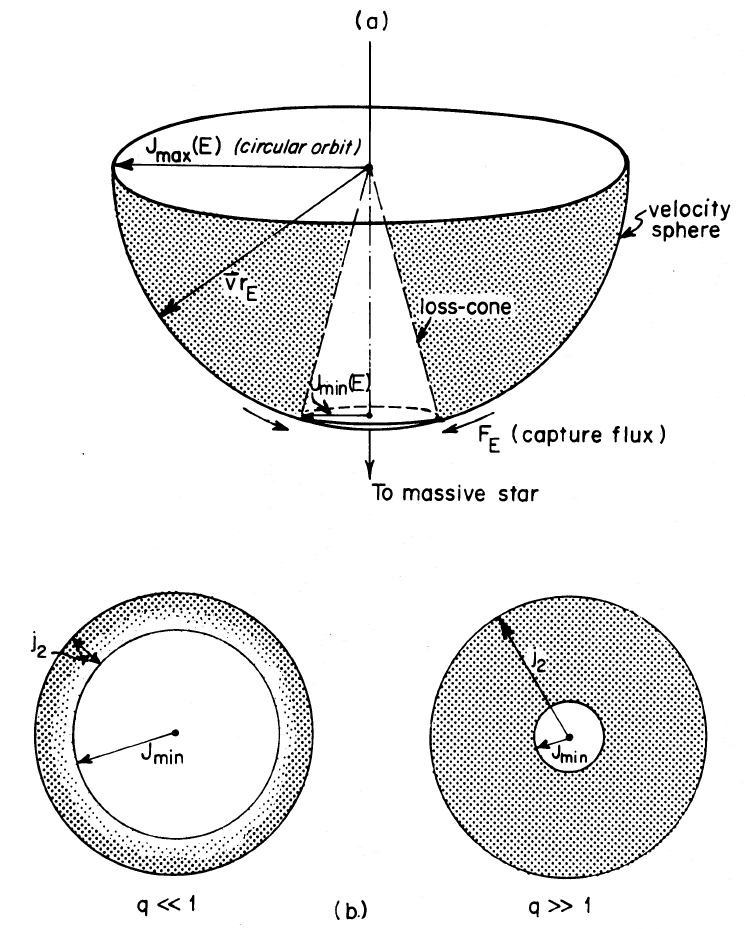
\includegraphics[width=0.5\linewidth]{Loss_cone.png}
    \caption{Fig. 1(a).—Velocity distribution of stars with fixed energy $E$;$J$ varies accordingly to the direction of $\mathbf{v}$ emphasising the two-dimensional nature of the problem. The vertical axis points towards the compact object of mass $M$.
Fig. 1(6).—The velocity sphere viewed from below. On the left the empty loss cone scenario; stellar density is nearly indipendent of $J$ everywhere but $J\gtrsim J_{min}$ where is quickly declines. On the right the full loss cone regime; consumed stars are immediately replenished by stars from a region much more extended- and uniform density- than the loss cone itself (the “pinhole” limit).}
    \label{loss cone image}
\end{figure}









\section{Gravitational Radiation from Black Hole Binaries}





\subsection{Linearized Gravitational Field Equation}

The starting point of the theoretical derivation of GWs properties, such as the energy and angular momentum they transport, from BH binary and the associated back-reaction on the astrophysical source, is the linearization of  field equations of Generl Relativity (GR)
\begin{equation}\label{Einstein field eq.}
    R_{\mu \nu}-\frac{1}{2}g_{\mu \nu} R=\frac{8\pi G}{c^4}T_{\mu \nu}.
\end{equation}
These constitute ten coupled, non-linear, second-order partial differential equations for the metric tensor; neverthless, they are not sufficient to uniquely set the ten indipendent components of $g_{\mu\nu}$ due to the four  Bianchi identities, equivalent to the same number of differential constraints, resulting in six  independent equations only. These four degrees of freedom are intimately connected to gauge symmetries, reflecting the arbitrariness of the four coordinates $x^\mu$ used to represent and solve Equation (\ref{Einstein field eq.}).\\To show how gravitational radiation emerges from Equation (\ref{Einstein field eq.}), we need to expand it around the Minkowski metric $\eta_{\mu \nu}=diag(-1,+1,+1,+1)$; therefore we assume
\begin{equation}
    g_{\mu \nu}(x)=\eta_{\mu \nu}+h_{\mu \nu}(x),
\end{equation}
with $|h_{\mu \nu}|\ll1$ being a symmetric tensor representing a small perturbation of the flat spacetime.\\The left-hand side of Equation (\ref{Einstein field eq.}) encodes the geometry and curvature of spacetime and contains all terms that are functions of the metric; in terms of the affine connection
\begin{equation}\label{affine connection def}
    \Gamma^\lambda _{\mu\nu}=\frac{1}{2}g^{\lambda \rho}(\partial_\mu g_{\nu\rho}+\partial_\nu g_{\rho\mu}-\partial_\rho g_{\mu\nu})
\end{equation}
and the Riemann tensor
\begin{equation}\label{Riemmann tensor def}
    R_{\lambda\mu}{}^{\rho}{}_{\nu}=\partial_\lambda \Gamma_{\mu\nu}^\rho-\partial_\mu \Gamma_{\lambda\nu}^\rho+\Gamma_{\lambda\sigma}^\rho \Gamma_{\mu\nu}^\sigma-\Gamma_{\mu\sigma}^\rho \Gamma_{\lambda\nu}^\sigma,
\end{equation}
they can be expressed indeed as 
\begin{equation}\label{Ricci tensor def}
    R_{\mu\nu}=R_{\sigma\mu}{}^{\sigma}{}_{\nu}
\end{equation}
and 
\begin{equation}\label{Ricci scalar def} R=g^{\alpha\beta}R_{\alpha\beta}=R_\sigma^\sigma.
\end{equation}
On the right-hand side, instead, appears the Energy-Momentum tensor; it can be read as the source term of the gravitational field equations and turns out to be
\begin{equation}\label{Energy-Momentum tensor def}
    T^{\mu\nu}=(\rho+p/c^2)u^\mu u^\nu+pg^{\mu\nu}
\end{equation}
for a perfect fluid of density $\rho$, pressure $p$ and four-velocity $v^\mu$.\\It straightforward to prove that, to the first order in the metric perturbation, they become:
\begin{equation}\label{linearized Ricci tensor}
    R_{\mu \nu}=-\frac{1}{2}(\Box h_{\mu \nu}+\partial_\mu \partial_\nu h-\partial_\lambda\partial_\mu h_\nu^\lambda-\partial_\nu\partial_\lambda h_\mu^\lambda)
\end{equation}
 and
\begin{equation}\label{linearized ricci scalar}
    R=\partial_\mu \partial_\nu h^{\mu\nu}-\Box h,
\end{equation}
where $h$ denotes $h_{\mu \nu}$ trace.\\Defining the so-called "trace reverse" of $h_{\mu\nu}$
\begin{equation}\label{trace reverse definition}
    \bar{h}_{\mu\nu}\equiv h_{\mu\nu}-\frac{1}{2}\eta_{\mu\nu} h
\end{equation}
and plugging the terms of Equations (\ref{linearized Ricci tensor}) and (\ref{linearized ricci scalar}) into Equation (\ref{Einstein field eq.}), the field equations take the form
\begin{equation}\label{linearized Einstein Eq. LONG}
    \Box \bar{h}_{\mu\nu} + \eta_{\mu\nu}\partial_\alpha\partial_\beta \bar{h}^{\alpha\beta}-\partial_\mu\partial_\lambda \bar{h}^\lambda_\nu-\partial_\nu\partial_\lambda \bar{h}^\lambda_\mu=-\frac{16\pi G}{c^4}T_{\mu\nu}.
\end{equation}
Taking advantage of the gauge freedom of Equation (\ref{Einstein field eq.}), it can be performed an infintesimal coordinate transformation of the kind
\begin{equation}
    x^\mu \rightarrow{}x'^\mu=x^\mu+\xi^\mu(x);
\end{equation}
as tensors obey to precise law of transformation, this yields
\begin{equation}
    \bar{h}'_{\mu\nu}=\frac{\partial x^\alpha}{\partial x'^\mu}\frac{\partial x^\beta}{\partial x'^\nu}\bar{h}_{\alpha\beta}\approx \bar{h}_{\mu\nu}-\partial _\mu \xi_\nu -\partial_\nu \xi_\mu+\eta_{\mu\nu}\partial_\sigma\xi^\sigma.
\end{equation}
Yet, if the four functions $\xi^\mu$ are chosen so as to satisfy the so-called De Donder gauge condition, i.e. $\Box\xi^\mu=\partial_\sigma\bar{h}^{\sigma\mu}$, then $\partial_\sigma\bar{h}'^{\sigma\mu}=0$ and, dropping the prime, Equation (\ref{linearized Einstein Eq. LONG}) semplifies to
\begin{equation}\label{linearized Einstein eq + gauge condition}
\begin{cases}
\Box \bar{h}_{\mu\nu} = -\dfrac{16\pi G}{c^4} T_{\mu\nu} \\
\partial_\mu\bar{h}^{\mu\nu}=0.
\end{cases}
\end{equation}
We are now ready to address the problem of determining  the general solution of the linearized Einstein's equations coupled with the De Donder gauge condition. 


\subsection{Generation and Propagation of Gravitational Waves}

To study the formation of GWs we initially focus on the solution of the problem defined in Equation (\ref{linearized Einstein eq + gauge condition}) inside the source where $T_{\mu\nu}\ne 0$.\\Linear partial differential equations solution can be obtained by the method of Green's function; by definition, the Green's function $G$ is the solution of the associated equation in case of a pont-like source, i.e.
\begin{equation}\label{Green equation}
    \Box_x G(x-x') = \delta^{(4)}(x-x'),
\end{equation}
with $\delta^{(4)}(x-x')$ being the four-dimensional Dirac function.\\It is relevant to note that, apart from the B.C. of the problem, $G$ depends only on the linear operator; therefore, from the radiation problem in electromagnetism, we already know that the proper solution is the retarded Green's function 
\begin{equation}\label{retarded Green function}
    G(x-x')=-\frac{1}{4\pi |\mathbf{x}-\mathbf{x'}|}\delta^{(4)}(ct_{ret}-ct'),
\end{equation}
where 
\begin{equation}\label{retarded time def}
    t_{ret}=t-\frac{|\mathbf{x}-\mathbf{x'}|}{c}
\end{equation}
is the time in past at which the radiation was emitted at $\mathbf{x'}$ in order to be observed at $\mathbf{x}$ at time $t$. Once the Green's function is found, the general solution will be the convolution between it and source term:
\begin{equation}\label{h_mn general solution}
    \bar{h}_{\mu\nu}(t,\mathbf{x})=\frac{4G}{c^4}\int d^3x'\frac{T_{\mu\nu}(t_{ret},\mathbf{x'})}{|\mathbf{x}-\mathbf{x'}|}.
\end{equation}
Prior to examining the formula reported in Equation (\ref{h_mn general solution}) and assessing which additional simplifications can be implemented and when they apply, it is appropriate to analyze how GWs propagate in vacuo.\\Outside the GWs source, $T_{\mu\nu}$ vanishes and, owing to the linearity of the d’Alembert operator, the solution can be expressed as superposition of plane waves without loss of generality, that is
\begin{equation}
    \bar{h}_{\mu\nu}(x)=\int d^3k (A_{\mu\nu}(\mathbf{k})e^{ik_\rho x^\rho}+c.c.)
\end{equation}
However, not all plane waves satisfy the linearized field equation in vacuo along with the gauge condition but linearity enables us to study the properties of a single plane wave separately; consequently, inserting the Ansatz $\bar{h}_{\mu\nu}\sim A_{\mu\nu}e^{ik_\rho x^\rho}$ yields the following two constraints:
\begin{enumerate}
    \item $(k_\rho k^\rho=0)$: the four-vector $k^\mu=(\omega/c,\mathbf{k})$ is a light-like vector (GWs travel at light speed $c$ in vacuo).
    \item $(k_\mu A^{\mu\nu}=0)$: it implies $A^{0\nu}=A^{3\nu}$ if we deal with GWs propagating along the $x^3$ direction, hence $k^\mu=(k,0,0,k)$.
\end{enumerate}
At this stage, the amplitude tensor $A^{\mu\nu}$ possesses six indipendet components --- ten, due to symmetry, reduced by the four constraints imposed by the gauge conditions --- and can be written as
\begin{equation}\label{A^mn 6 dof}   
A^{\mu\nu} =
\begin{pmatrix}
A^{00} & A^{10} & A^{20} & A^{00} \\
A^{10} & A^{11} & A^{12} & A^{10} \\
A^{20} & A^{12} & A^{22} & A^{20} \\
A^{00} & A^{10} & A^{20} & A^{00}
\end{pmatrix}.
\end{equation}
Out of the six polarizations shown in Equation (\ref{A^mn 6 dof}), four are unphysical because they vanish when the residual gauge freedom associated with four arbitrary harmonic functions $\xi^\mu$ is exploited. One is free to adopt functions proportional to the plane wave solutions of the vacuo problem, i.e. $\xi^\mu=\epsilon^\mu e^{ik_\rho x^\rho}$ are harmonic, and to set their amplitudes $\epsilon^\mu$ such that 
\begin{equation}\label{A^mn TT gauge}   
A^{\mu\nu}_{TT} =
\begin{pmatrix}
0 & 0 & 0 & 0 \\
0 & h_+ & h_x & 0 \\
0 & h_x & -h_+ & 0 \\
0 & 0 & 0 & 0
\end{pmatrix}.
\end{equation}
The coordinate system where $A^{\mu\nu}$ is in the form of Equation (\ref{A^mn TT gauge}), with two indipendent polarizations only, and defined by 
\begin{equation}
    \partial_\mu h^{\mu\nu}=0, \quad h^{0\mu}=0, \quad h^i_i=0,
\end{equation}
is referred to as "TT gauge"\footnote{In the TT gauge, according to the definition provided, $\bar{h}_{ij}^{TT}=h_{ij}^{TT}$.}.\\Having analyzed the propagation of GWs in vacuo and the properties of the TT gauge, we are now in the position to focus again on the source solution reported in Equation (\ref{h_mn general solution}). One of the greatest simplifications to this integral consists of the so-called "Compact-source approximation"; it applies outside the source whenever its size is negligible with respect to the source-detector separation. In this regime, we can retain the leading term of the multipole expansion only, thus
\begin{equation}\label{h_mn compact source solution}
    h_{ij}^{TT}(t,\mathbf{x})=\frac{4G}{c^4r}\int d^3x'T_{ij}(t_{ret},\mathbf{x'}).
\end{equation}
Furthermore, far from the source, the conservation of the Energy-Momentum tensor, namely $\nabla_\mu T^{\mu\nu}\approx\partial_\mu T^{\mu\nu}=0$, yields
\begin{equation}\label{h_mn final form}
    h_{ij}^{TT}(t,\boldsymbol{x})=\frac{2G}{rc^4}\ddot{Q}^{TT}_{ij}(t-r/c)
\end{equation}
at lowest order in the low-velocity expansion.\\The term $Q^{TT}_{ij}$ introduced in Equation (\ref{h_mn final form})\footnote{The components with at least one time index are excluded from our analysis because they are constant and therefore do not contribute to GWs formation.} is the representation of the quadrupole moment in the class of coordinate systems satisfying the TT gauge conditions; defining the quadrupole moment of $T^{00}/c^2=\rho$ as
\begin{equation}\label{M_ij definition}
    M^{ij}\equiv \frac{1}{c^2}\int d^3x T^{00}(t,\boldsymbol{x})x^ix^j,
\end{equation}
it is thus possible to write
\begin{equation}\label{Q_ij def}
    Q^{ij}\equiv M^{ij}-\frac{1}{3}\delta^{ij}M_{kk}=\int d^3x\rho(t,\mathbf{x})\left(x^ix^j-\frac{1}{3}r^2\delta^{ij}\right).
\end{equation}
Equation (\ref{h_mn compact source solution}) shows that, unlike electromagnetic radiation, at lowest order the gravitational radiation arises from changes in the quadrupole moment; other important observables such as the energy and angular momentum carried by GWs, needed to estimate the back-reaction, will be derived from the quantities defined in Equation (\ref{Q_ij def}) indeed.\\The energy and angular momentum conservation laws impose that the rates a which these quantities are carried away by GWs at time $t$ and at large separation $r$ from the source coincide with the corresponding rates of orbital energy ---if the emitting system consists of a BH binary--- and angular momentum, negletting the spin contribute, loss evaluated at the appropriate retarded time; in formulae:
\begin{equation}\label{energy loss rate by GWs}
    P_{quad}=\frac{dE_{gw}}{dt}=\frac{G}{5c^5}\langle\dddot{Q}_{ij}\dddot{Q}_{ij}\rangle=-\frac{dE_{source}}{dt},
\end{equation}
or equivalently in terms of $M_{ij}$
\begin{equation}\label{P_quad in terms of M_ij}
     P_{quad}=\frac{G}{5c^5}\left\langle\dddot{M}_{ij}\dddot{M}_{ij}-\frac{1}{3}(\dddot{M}_{kk})^2\right\rangle,
\end{equation}
and 
\begin{equation}\label{angular momentum loss rate by GWs}
    \frac{dL^i_{gw}}{dt}=\frac{2G}{5c^5}\epsilon^{ijk}\langle\ddot{Q}_{jl}\dddot{Q}_{kl}\rangle=-\frac{dL^i_{source}}{dt}.
\end{equation}
Equations (\ref{energy loss rate by GWs}) and (\ref{angular momentum loss rate by GWs}) will be of fundamental importance for estimating the back-reaction induced by GWs emission on the black hole binary.















\subsection{Gravitational Waves from Black Hole Binaries and Back-Reaction}
We now focus on the gravitational radiation emitted by two masses $m_1$ and $m_2$ moving along elliptic Keplerian orbit. Let $m=m_1+m_2$ and $\mu=m_1\cdot m_2/{m}$ be the total mass and the reduced mass respectively.\\Regardless of whether the orbit is bound or unbound, the motion of the two bodies takes place in a plane due to the conservation of the angular momentum $\mathbf{L}$; therefore, in this plane, the x-y plane, perpendicular to $\mathbf{L}$, it is convenient to  
introduce the polar coordinates $(r,\psi)$ with origin at center-of-mass.\\In this frame, as before denoted by $S_{CM}$, 
\begin{equation}\label{L of two body problem}
    L_z=\mu r^2\dot{\psi}
\end{equation}
coincides with the modulus $L$ of the costant vector while, as a consequence of the Köenig theorem,
\begin{equation}\label{E of two body problem}
    E=\frac{1}{2}\mu \dot{r}^2+\frac{L^2}{2\mu r^2}-\frac{Gm\mu}{r}
\end{equation}
exhibits only the term of kinetic energy corresponding to the relative motion of the system, as in $S_{CM}$ holds $K_{CM}=0$ by definition.\\The integration of Equation (\ref{E of two body problem}) requires, as in \parencite{Capozziello_2008}, the introduction of the auxiliary variable $w(\psi)=1/r(\psi)$; plugging it into the energy conservation identity, Equation (\ref{E of two body problem}) becomes 
\begin{equation}
    w'^2+w^2-\frac{2Gm_1m_2\mu}{L^2}w=\frac{2\mu E}{L^2}
\end{equation}
where $w'\equiv dw/d\psi$. Differentiating both sides of the last equation with respect to $\psi$ leads to
\begin{equation}\label{u differential equation}
    w'\left(w''+w-\frac{Gm_1m_2\mu}{L^2}\right)=0.
\end{equation}
Apart from the solution $w=const$, corresponding to a circular binary, the problem admits harmonic–oscillator–like and, upon solving for $r(\psi)$, it is found to be given by
\begin{equation}\label{two-body solution}
    r(\psi)=\frac{R}{1+e\cos{\psi}},
\end{equation}
with $R=L^2/(Gm\mu^2)$ being semi-latus rectum --- the polar axis is aligned to the major axis $2a$, so that 
$R$ corresponds to the distance between the origin and the point of the conic at $\psi=\pi/2$--- and is related to the eccentricity $e$ by 
\begin{equation}\label{eccentricity formula}
    e^2=1-\frac{R}{a}=1+\frac{2EL^2}{G^2m^2\mu^3}.
\end{equation}
It is worth of noticing that we are interested in the GWs emission process by a BH binary, which is by definition a gravitationally bound system; therefore, from this point onward it will be assumed $E<0$ and thus, by virtue of Equation (\ref{eccentricity formula}), $0\le e<1$.
Since the two semiaxes are given by
\begin{equation}\label{a and b as a function of e}
    a=\frac{R}{1-e^2} \qquad \qquad b=\frac{R}{\sqrt{1-e^2}},
\end{equation}
inserting Equation (\ref{eccentricity formula}) into the first identity of Equation (\ref{a and b as a function of e}) gives the semi-major axis in terms of $E$; explicitly:
\begin{equation}\label{a as a function of E}
    a=-\frac{Gm\mu}{2E}
\end{equation}
It follows that fixing the energy means setting the semi-major axis.\\The functions $r(t)$ and $\psi(t)$ can be obtained by direct integration of Equations (\ref{L of two body problem}) and (\ref{E of two body problem}); they are usually given in the parametric form
\begin{equation}
    r(t)=a[1-e\cos{u(t)}] \qquad \qquad\psi(t)=\frac{\cos{u(t)}-e}{1-e\cos{u(t)}}
\end{equation}
in terms of the "eccentric anomaly" $u$ defined in the famous Kepler equation
\begin{equation}
    u(t)-e\sin{u(t)}=\left(\frac{Gm}{a^3}\right)^{1/2}t\equiv \omega_0 t.
\end{equation}
The transformation from from polar cordinates $(r,\psi)$ to Cartesian ones $(x,y)$ is illistrated below
\begin{equation}
\begin{cases}
x = r \cos\psi = a\left[\cos u(t) - e\right] \\
y = r \sin\psi = b \sin u(t) .
\end{cases}
\end{equation}
We now possess all the necessary ingredients to proceed with the computation of the rates of energy and angular momentum carried by GWs, which will play a fundamental role in assessing the back-reaction on the binary system.\\In the reference system $S_{CM}$ holds $\rho(t,\mathbf{x})=\mu\delta(x-r\cos{\psi})\delta(y-r\sin{\psi})\delta(z)$
and, according to \\Equation (\ref{M_ij definition}), it is immediate to get
\begin{equation}
M_{ij} = \mu r^2(t)\begin{bmatrix}
\cos^2(\psi) & \sin{(\psi)\cos(\psi)} \\
\sin{(\psi)\cos(\psi)} & \sin^2(\psi)
\end{bmatrix}.
\end{equation}
The time derivatives are easier computed when $r$, which is a function of time itself, is expressed as a function of $\psi$; this is accomplished by replacing this variable with the general solution of the two-body problem provided by Equation (\ref{two-body solution}). A simple computation returns the third time derivatives needed to derive the power radiated in the quadrupole approximation, i.e.
\begin{equation}\label{d3M _11/dt3}  
\dddot{M}_{11} = \beta (1 + e \cos \psi)^2 \left[ 2 \sin 2\psi + 3e \sin \psi \cos^2 \psi \right],
\end{equation}

\begin{equation}\label{d3M _22/dt3}  
    \dddot{M}_{22} = \beta (1 + e \cos \psi)^2 \left[ -2 \sin 2\psi - e \sin \psi (1 + 3 \cos^2 \psi) \right],
\end{equation}


\begin{equation}
    \dddot{M}_{12} = \beta (1 + e \cos \psi)^2 \left[ -2 \cos 2\psi + e \cos \psi (1 - 3 \cos^2 \psi) \right],
\end{equation}
where the factor $\beta$ is defined as
\begin{equation}
\beta^2 \equiv \frac{4 G^3 \mu^2 m^3}{a^5 (1 - e^2)^5}. 
\end{equation}
By means of Equation (\ref{energy loss rate by GWs}) we get in conclusion
\begin{equation}
    P(\psi)=\frac{8G^4}{15c^5}\frac{\mu^2m^3}{a^5(1-e^2)^5}(1+e\cos(\psi))^4[12(1+e\cos(\psi))^2+e^2\sin^2(\psi)].
\end{equation}
However, we recall that this istantaneous quantity is not constant over one orbital period for elliptic Keplerian orbits as in general $M_{ij}$ will suffer from different rate of variation from pericenter to apocenter; therefore, taking the temporal average over one orbital period, $T\equiv2\pi/\omega_0$ returns
\begin{equation}\label{P of GWs binary}
    P\equiv\frac{1}{T}\int_0^T dtP(\psi)=\frac{\omega_0}{2\pi}\int_0^{2\pi} d\psi \frac{P(\psi)}{\dot{\psi}}=\frac{32G^4\mu^2m^3}{5c^5a^5}F(e),
\end{equation}
with 
\begin{equation}\label{F(e) definition}
    F(e)=\frac{1}{(1-e^2)^{7/2}}\left(1+\frac{73}{24}e^2+\frac{37}{96}e^4\right)
\end{equation}
being a function strongly depending on the eccentricity, which reduces to unity in case of circular binary.\\Throughout the inspiral phase, the binary radiates not only energy but angular momentum as well, carried by GWS, and undergoes secular changes in both semimajor axis and ellipticity until coalescence eventually occurs. Therefore, another key ingredient in evaluating the back-reaction on the binary evolution is the determination of the angular momentum loss rate. It is quantified in Equation (\ref{angular momentum loss rate by GWs}) which becomes
\begin{equation}\label{angular momentum loss rate in terms of M_ij}
    \frac{dL^i_{source}}{dt}=-\frac{2G}{5c^5}\epsilon^{ikl}\left<\dddot{M}_{ka}\dddot{M}_{la}\right>
\end{equation}
as the the terms of the form $\epsilon^{ijk}\delta_{jl}\dddot{Q}_{kl}$ vanish, since they correspond to the contraction of an antisymmetric tensor with a symmetric one.\\Taking into account that, in $S_{CM}$, all components $M_{i3}$ are identically zero and that $L=L_z=L^3_{source}$, one can rewrite Equation (\ref{angular momentum loss rate in terms of M_ij}) in a more convenient form consistent with the previous arguments:
\begin{equation}
    \frac{dL}{dt}=\frac{4G}{5c^5}\langle \ddot{M}_{12}(\dddot{M}_{11}-\dddot{M}_{22})\rangle.
\end{equation}
The last identity provides $dL/dt$ in terms of the second and third derivatives of the quadrupole moment of $\rho$; although the second derivative $\ddot{M}_{12}$ has not been computed explicitly yet, it follows straightforwardly from the same procedure used to derive $\dddot{M}_{ij}$, hence
\begin{equation}\label{d2 M_12/dt2}
\ddot{M}_{12}
=
\frac{G \mu m}{a(1 - e^2)} \sin \psi
\left[
-4(1 + e \cos \psi)^2 \cos \psi
+ 2e \left( 3 \cos^2 \psi - 1 + 2e \cos^3 \psi \right)
\right].
\end{equation}
Yet, adopting the expressions for reported in Equations (\ref{d3M _11/dt3}), (\ref{d3M _22/dt3}) and (\ref{d2 M_12/dt2}) respectively, we get the angular momentum loss, corresponding to minus the angular momentum carried by the gravitational radiation in the quadrupole approximation; then, the temporal average over a single orbital period $T$, transformed into an integral over the angular position $\psi$, returns
\begin{equation}
    \frac{dL}{dt}=-\frac{32}{5}\frac{G^{7/2}\mu^2m^{5/2}}{c^5a^{7/2}}\frac{1}{(1-e^2)^2}\left(1+\frac{7}{8}e^2\right)
\end{equation}
Lastly, the simi-major axis and eccentricity evolution of the BH binary results by imposing the conservation of the energy and angular momentum of the system composed of the binary and GWs; differentiating Equations (\ref{eccentricity formula}) and (\ref{a as a function of E}) with respect to the time yields
\begin{equation}
    \frac{da}{dt}=\frac{Gm\mu}{2E^2(a)}(-P)
\end{equation}
and
\begin{equation}
    2e\frac{de}{dt}=\frac{2}{G^2m^2\mu^3}\left[-PL^2(a,e)+2E(a)L(a,e)\frac{dL}{dt}\right].
\end{equation}
By rearranging all the terms and performing the appropriate substitutions, \textcite{Peters_1963} gave 
\begin{equation}\label{da/dt Peterson}
    \frac{da}{dt} = -\frac{64}{5} \frac{G^3 \mu m^2}{c^5 a^3} \frac{1}{(1 - e^2)^{7/2}} \left( 1 + \frac{73}{24}e^2 + \frac{37}{96}e^4 \right)
\end{equation}
along with
\begin{equation}\label{de/dt Peterson}
    \frac{de}{dt} = -\frac{304}{15} \frac{G^3 \mu m^2}{c^5 a^4}  \frac{e}{(1 - e^2)^{5/2}} \left( 1 + \frac{121}{304}e^2 \right)
\end{equation}
that has been employed by \textcite{Quinlan_1996} and \textcite{Sesana_2010} in order to reconstruct evolutionary tracks of BH binaries through a "Hybrid model", which will be described later.\\Equations (\ref{da/dt Peterson}) and (\ref{de/dt Peterson}) prove that GWs emission  is efficient, more precisely at little binary separation due to $a^{-3}$ and $a^{-4}$ dependence respectively, not only in shrinking the BHs pair, by extracting orbital energy, but in promoting the orbit circularization as well, thus making this mechanism dominant over stellar scattering at late stage of binary inspiral.\\Furthermore, another key piece of information that can be derived from the theory is the expected coalescence time $\tau$ of the binary in the case of gravitational-wave emission alone. This should reproduce the characteristic hardening timescale of the final stage, when orbital shrinking driven by gravitational radiation takes over stellar scattering. This is obtained by combining Equations (\ref{da/dt Peterson}) and (\ref{de/dt Peterson}); this mathematical operation leads to a differential equation for $a=a(e)$, which reads
\begin{equation}\label{da/de Maggiore}
    \frac{da}{de}=\frac{12}{19}\frac{1+\frac{73}{24}e^2+\frac{37}{96}e^4}{e(1-e^2)\left(1+\frac{121}{304}e^2\right)}.
\end{equation}
The last equation admits analytic solution of the kind
\begin{equation}\label{a=a(e) Maggiore}
    a(e)=a_0\frac{g(e)}{g(e_0)}
\end{equation}
where 
\begin{equation}\label{g(e) Maggiore}
    g(e)=\frac{e^{12/19}}{1-e^2}\left(1+\frac{121}{304}e^2\right)^{870/2299}
\end{equation}
and $(a_0,e_0)$ denotes the initial point of the of binary evolutionary track.\\Last but not least, given the BH binary initial condition $(a_0,e_0)$, the coalescence time is found by integration over the eccentricity and by noticing that, if we set $(a(0),e(0))=(a_0,e_0)$, $e(\tau)=0$ due to orbit circularization:
\begin{equation}\label{tau coal. analytical}
\tau(a_0,e_0)=\int_0^{\tau(a_0,e_0)}dt=\int_{e_0}^{0}de \frac{dt}{de}=\int_{e_0}^{0}de \frac{a^4(e)(1-e^2)^{5/2}}{e\left(1+\frac{121}{304}e^2\right)}.
\end{equation}
By substituting Equation (\ref{a=a(e) Maggiore}) into Equation (\ref{tau coal. analytical}) one gets the final expression
\begin{equation}\label{t_coal Maggiore} 
\tau_{\mathrm{coal}}(a_0,e_0)
=
\frac{12}{19}
\frac{c^5}{G^3}
\frac{a_0^4}{\mu m^2}
\int_{0}^{e_0}
\frac{e^{29/19}
\left(1+\frac{121}{304}e^2\right)^{1181/2299}}
{(1-e^2)^{3/2}}
\,\mathrm{d}e.
\end{equation}









\chapter{A Hybrid Approach to Binary Evolution}



\section{Quinlan Formalism}
\subsection{Introduction}
In this work, binary evolution embedded in a fixed stellar background problem is addressed in a hybrid fashion providing a self consistent analytical framework where dimensioless rates are directely estimated from scattering experiments.\\Scattering experiments are carried out for the restricted three-body problem and proceed until either the binary coalesce or stellar ejection has become so important that the host galaxy can no longer be considered fixed.\\Three dimensionless quantities $(H,K,J)$ are measured from numerical experiments and defined as:
\begin{equation}\label{H Q96}
    H=\frac{\sigma}{G\rho}\frac{d}{dt}\left(\frac{1}{a}\right),
\end{equation}

\begin{equation}\label{K Q96}
    K=\frac{de}{d\ln({1/a})}
\end{equation}
and 
\begin{equation}\label{J Q96}
    J=\frac{1}{M_{12}}\frac{dM_{ej}}{d\ln({1/a})}.
\end{equation}
Equations (\ref{H Q96}), (\ref{K Q96}) and (\ref{J Q96}) introduce the so called dimensionless hardening
rate H, eccentricity growth rate K and mass loss rate. Once $(H,J,K)$ are obtained from scattering experiments, the system of coupled differential equations can be solved for the binary semi-major axis, eccentricity and ejected mass time derivatives and numerical methods will eventually return their evolution within the fixed galaxy model of interest.



\subsection{Quinlan Scattering Experiments}
Although stars approach the binary with a wide velocity distribution, consistent with the adopted $\sigma$, simulations are performed considering a unique value of the velocity at infinity (thus are $\mathbf{UNBOUND}$) then accounting for a Maxwellian distribution \cite{Quinlan_1996}.\\This semplification leads to the estimate of the so called $H_1(v)$ first, which thus allows to obtian $H(\sigma)$ by integration over all possible velocities and weighted by MB distribution.\\Therefore from each scattering experiment is measured the dimensionless energy change 
\begin{equation}\label{C quinlan}
    C=\frac{a\Delta E_*}{G\mu}
\end{equation}
and is then avereged over binary orientation $(4\pi)$ and phase $(2\pi)$.\\By introducing the quantity
\begin{equation}
    b_0^2=\frac{2GM_{12}a}{v^2}
\end{equation}
in order to work with the dimensionless impact parameter $x=b/b_0$, finally:
\begin{equation}
    H_1=\frac{1}{\pi b_0^2}\int db2\pi b 4 \pi \langle C\rangle=8 \pi \int dx\quad x \langle C\rangle\equiv8\pi I_x(C).
\end{equation}
Similarly, assuming a given velocity for scattering experiments, the eccentricity growth rate $K$ is obtained from $K_1$.\\The differentiation of
\begin{equation}
    e^2=1+\frac{2EL^2}{\mu(GM_{12})^2}
\end{equation}
returns
\begin{equation}
    \frac{\Delta e}{\Delta ln(1/a)}=\frac{1-e^2}{2e}\left[-2\left(\frac{E}{\Delta E}\right)\left(\frac{\Delta L_z}{L_z}\right)-1\right]=\frac{1-e^2}{2e}(B-C),
\end{equation}
where B is the dimensionless angular momentum change defined as 
\begin{equation}\label{B quinlan}
    B\equiv-\frac{M_{12}}{m_*}\frac{\Delta L_z}{L_z}.
\end{equation}
Finally, integrating over all possible impact parameter, angles and normalizing the result, $K_1$ can be computed as
\begin{equation}
    K_1=\frac{\int dx\quad xC(x)\langle \frac{\Delta e}{\Delta ln(1/a)}\rangle}{\int dx\quad xC(x)}=\frac{(1-e^2)}{2e}\left[\frac{I_x(B-C)}{I_x(C)}\right].
\end{equation}
$\mathbf{NOTE}$:During three-body encounters, star-binary energy and angular momentum exchange ensures the conservation of both of them; thus the binary evolution can be inferred from stellar orbial properties evolution.


The initial setup of each scattering experimet is completely fixed by the following $d=5$ uniformly distributed- within a proper interval- parameters :
\begin{enumerate}
    \item $b^2$ rather than $b$ because $t_{coll}\propto \lambda\propto \sigma^{-1}\propto b^{-2}$. Thus reproducing correctly the encounter rate.
    \item  cosine of the inclination: angle between binary $\mathbf{L}$ and $\mathbf{v}(-\infty)$.
    \item  longitude of ascending node: azimuthal angle of $\mathbf{v}(-\infty)$ in $\mathbf{L}$ equatorial plane
    \item  the argument of pericenter (point of closest approach): it fixes ellipse orientation over the orbital plane
    \item  the mean anomaly to specify BHs position along the ellipse at a given time.

\end{enumerate}

Once these parameters are drawn and convinient coordinates are adopted, the numerical integration starts at binary-star separation $r=50a$ and is stopped when the star leaves this sphere around the binary with posity energy, hence recording the main quantities of interest.\\Systematic errors arise from approximations used in order to semplify the numerical simulation, for istance: assuming keplerian orbit outside that sphere, thus stopping at zero order term in multipole expansion.\\Statistical errors in any average quantity scale, at large number of scatterings N, as $(ln\quad N)^d/N$ because quasi-random numbers are used.\\$H_1$ is measured for a wide range of masses ratio and eccentricity and fitted with the two free-parameters model
\begin{equation}
    H_1(v)=H_0(1+(v/w)^4)^{-1/2}.
\end{equation}




$\mathbf{NOTE}$: "This fits the data well at high and low velocities. It does not fit so well when $H_1$ first starts to decrease"

Similarly $K_1$ is derived as a function of "e" and fitted with the following three parameters model:
\begin{equation}
    K_1(e)=e(1-e^2)^{k_0}(k_1+k_2e)
\end{equation}
$\mathbf{NOTE}$: $H_1$ is a function of v only while $K_1$ on both e and v.


All free parameters are obtained for different masses ratio.


\begin{figure}
    \centering
    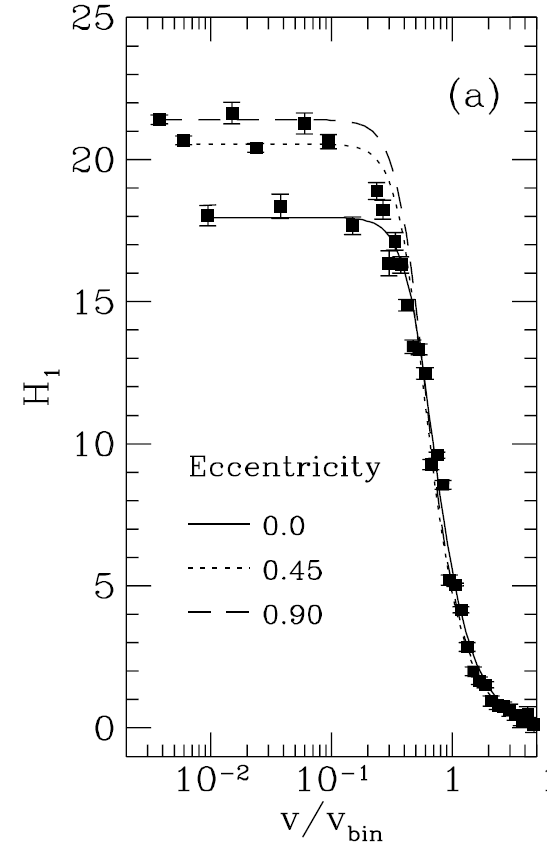
\includegraphics[width=0.5\linewidth]{H_1.png}
    \caption{This plot shows that $H_1$ is almost indipendet of the eccentricity.}
    \label{H_1 quinlann}
\end{figure}

$\mathbf{NOTE:}$ in Sesana 2010, Fig \ref{H_1 quinlann} is reported as H vs a but this agrees with the functional form of $H_1$ and $V_{bin}=\sqrt{GM_{12}/a}$.\\Therefore, the hardening rate for a circular binary have been used for all eccentricities.

\subsection{Aplication to a galaxy model}
Once stellar density $\rho$ and velocity dispersion $\sigma$ are specified, the binary BH is introduced at center of the system with a given initial eccentricity $e_0$ and separation $a_0$ such that $V_{bin}=\sigma/5$.\\The last  corresponds to a condition about $a_0$ which is model indipendent and for the binary to be soft at beginning of the integration; a BH binary is indeed called hard 
if it hardens at a constant rate, that is if $\sigma\ll \omega$ or equivalently
if $V_{bin}/\sigma \gg (1+m_1/m_2)^{1/2}$.\\Peters (1964) equation for gravitational wave emission
\begin{equation}
    \frac{da}{dt} = -\frac{64}{5} \frac{G^3 \mu m^2}{c^5 a^3} \frac{1}{(1 - e^2)^{7/2}} \left( 1 + \frac{73}{24}e^2 + \frac{37}{96}e^4 \right)
\end{equation}

\begin{equation}
    \frac{de}{dt} = -\frac{304}{15} \frac{G^3 \mu m^2}{c^5 a^4}  \frac{e}{(1 - e^2)^{5/2}} \left( 1 + \frac{121}{304}e^2 \right)
\end{equation}
are considered as well in order to compute $da/dt$ and $de/dt$.\\Despite $dM_{ej}/dt$ is computed, a and e evolution can be assumed to occur in a fixed background whenever this is negligible; the ejected mass hardly exceeds a few times $M_{12}$.\\Neverthless, the stellar mass ejection makes the binary hardening less and less efficient; once nearby stars are expelled, the hardening rate depends on the diffusion of stars back into the "Loss cone" due to two-body relaxation.\\If stars removal is efficient, correction to the density profile must be applied assuming a given rate for the process above.\\Fig.\ref{a and e quinlan} shows that the binary evolves mainly through three phases separated by two trashold destances:\begin{enumerate}
    \item $a_h=\frac{Gm_2}{4\sigma^2}$
    \item $a_{gw}$
\end{enumerate}
Quasi-circular binaries ($e_0<0.3$) remain circular with little e-growth before entering the GWs emission domain, while eccentricity increment is more important if $e_0>0.3$.






\newpage
\begin{figure}
    \centering
    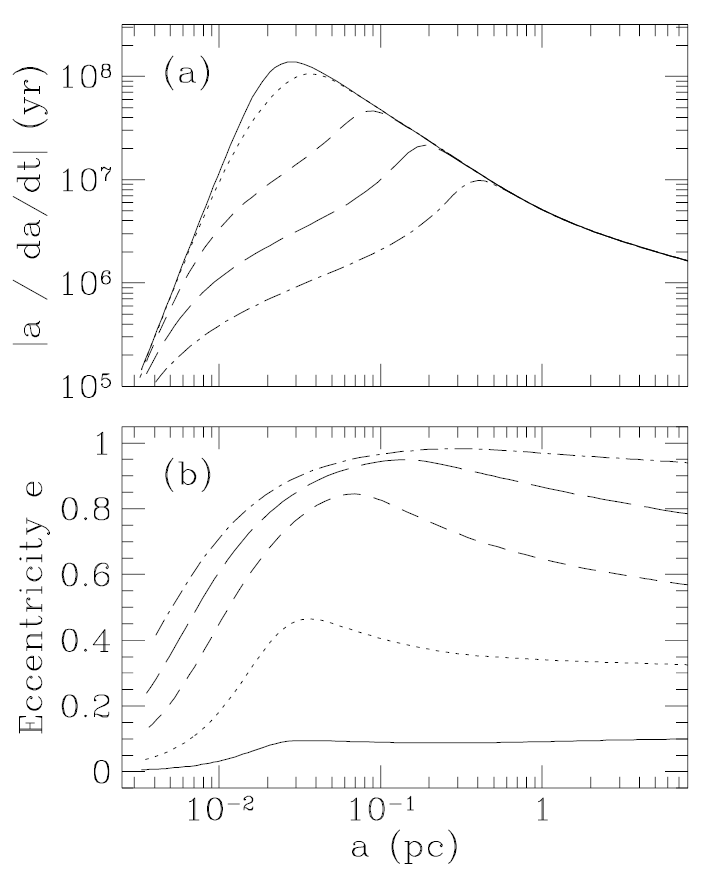
\includegraphics[width=0.5\linewidth]{a_and_e_quinlan.png}
    \caption{Eccentricity evolution. The solid line is the same as
in Fig. 7(a); the other lines assume initial eccentricities of 0.3
(dotted), 0.5, 0.7, and 0.9 (dashed-dotted).}
    \label{a and e quinlan}
\end{figure}




\section{Sesana Hybrid Model}

\subsection{Sesana Scattering Experiments}
This work \cite{Sesana_2006} is aimed at unvieling by  full three-body scattering experiments how a population of HVS form as a result of the interaction between a MBHB and ambient stars, unbound to the binary, drawn from a MB distribution . Other than the dynamical properties of these HVS, binary hardening, mass ejection rate and eccentricity growth rate $(H,J,K)$ are tracked by numerical simulations.\\Dynamical friction is efficient (especially in wet major mergers) in dragging two  massive BHs towards the innermost region of the new formed galaxy; over the time scale $t_{df}$ the binary forms and hardens  through gravitational slingshot, hence ejecting low angular momentum stars passing close to the binary. \\Following Q96 approach, the equations defining $(H,J,K)$ are (\ref{H Q96}),(\ref{J Q96}) and (\ref{K Q96}).\\At odds with Q96, where three-body scattering experiments are conducted for a fixed impact velocity, varying the binary separation and then averaging over the Maxwellian distribution, now the separation is fixed, i.e. $V_c=(GM_{12}/a)^{1/2}=const$, and the quantity $v/V_c$ is sampled over four decades, corresponding to a sampling of about four decades in binary separation.\\Each run is set by the inital configuration, corrseponding to a point in the parameter space $(q,e_0)$; the combination of binary masses ratio $q=1,1/3,1/9,1/27,1/81,1/243$ and initial eccentricity $e_0=0.01,0.3,0.6,0.9$ leads to 24 runs, involving $4\cdot10^6$ stars each.\\The (Maxwellian averaged) rates H, J,
and K derived from scattering experiments are fitted by the following functions


 \begin{equation}
     H=A(1+a/a_0)^\gamma
\end{equation}

 \begin{equation}
    J=A(a/a_0)^\alpha [(1+(a/a_0)^\beta]^\gamma
\end{equation}

\begin{equation}
    K=A(1+a/a_0)^\gamma+B.
\end{equation}

\begin{figure}
    \centering
    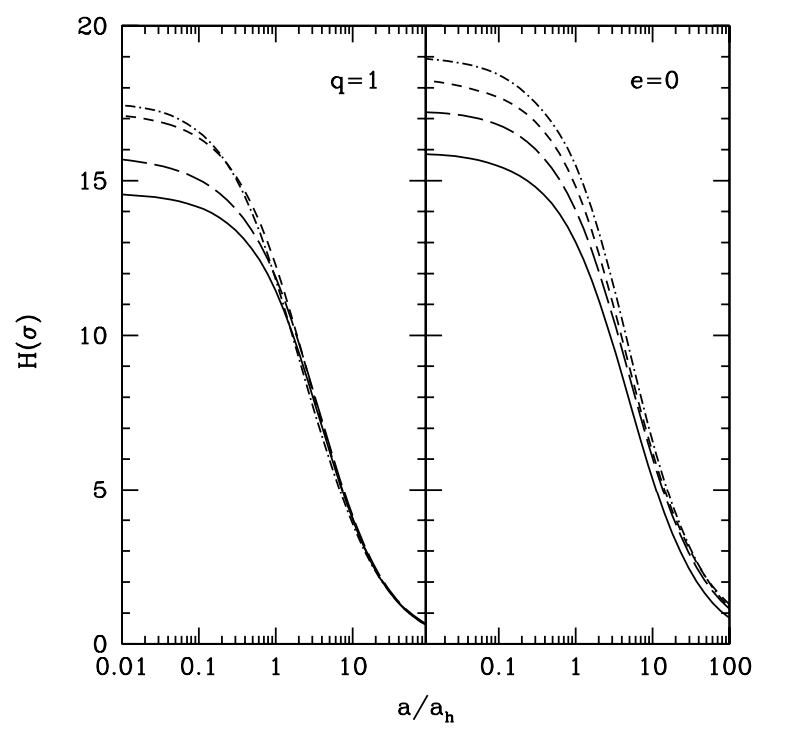
\includegraphics[width=0.5\linewidth]{H_Sesana2006.png}
    \caption{Binary hardening rate H (averaged over a Maxwellian velocity
distribution) vs. $a/a_h$. Left: $e= 0, 0.3, 0.6, 0.9$ for $q=1$. Right: q ¼ 1/3, 1/9,
1/27, and 1/81 for e ¼ 0. Line style as in Fig. 1}
    \label{H Sesana 2006}
\end{figure}


\begin{figure}
    \centering
    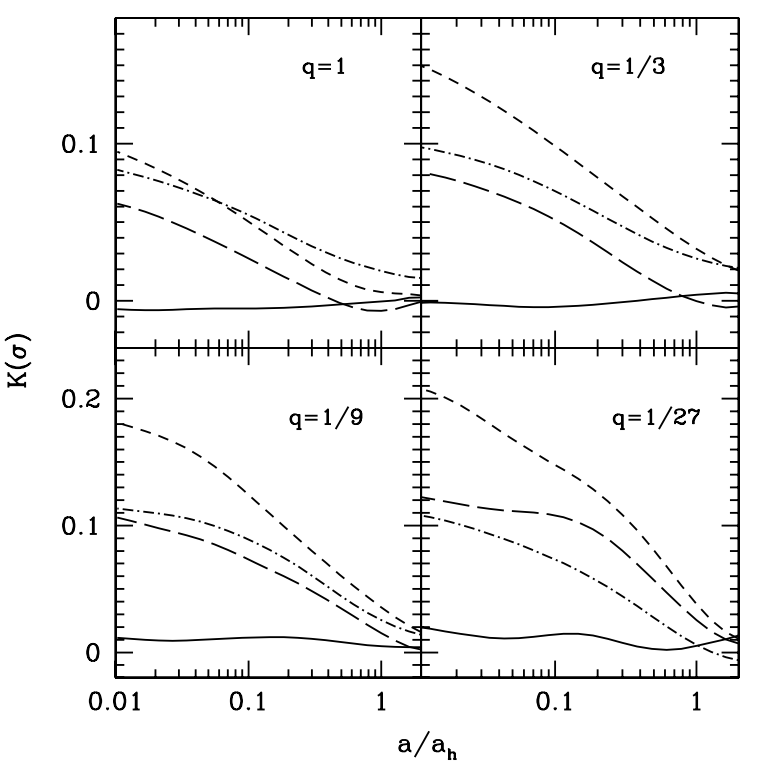
\includegraphics[width=0.5\linewidth]{K_Sesana2006.png}
    \caption{Eccentricity evolution. The solid line is the same as
in Fig. 7(a); the other lines assume initial eccentricities of 0.3
(dotted), 0.5, 0.7, and 0.9 (dashed-dotted).}
    \label{K Sesana 2006}
\end{figure}
Figure \ref{H Sesana 2006} shows that the hardening rate is nearly constant when $a<a_h$, in perfect agreement with Q96 results. Therefore hard binary can be characterised by a costant hardening rate. Additionally, $H$ decreases with $q$ (asymmetric binaries harden faster) and increases with eccentricity (circular binaries harden more slowly).\\As reported in Figure \ref{K Sesana 2006}, $K$ is close to zero at any binary separation for circular binary; if the binary is eccentric at $a_h$ already, then K (and $e$) increases monotonically with binary shrinking.\\$\mathbf{NOTE}$: in this paper the binary shrinking is studied taking into account gravitational slingshot on UNBOUND stars passing close to binary and ejected at higher velocity. In particular:
\begin{enumerate}
    \item the ejection criterion relies on the stellar background model (here SIS stellar Bulge is considered)
    \item The stellar background is assumed to be fixed; this approximation holds if the ejected mass does not exceed a trashold
    \item Binary shrinking requires low angular momentum stars as they havo to pass closer and closer to the binary BHs for slingshot to be effective; however from $a<a_h$ the fraction of stars with these properties, populating the so called "Loss cone", is very small. Being depletd by three-body encounters, binary hardening when binary is hard depends on the efficiency of loss cone refilling.
\end{enumerate}
 
Bound stars \cite{Sesana_2008}     ,\cite{Sesana_2010}
\newpage
\subsection{Sesana 2010 Results and  Comparison}
As confirmed by observations of galaxies hosting a dynamically evolved BH binary, stellar scouring by binary hardening seems to imprint an inner cusp to the original stellar background. Motivated by this emerging picture, Sesana \cite{Sesana_2010} adopted a stellar density profile matching a SIS outside the binary influence radius $r_{inf}$ and a power low distribution inside; in formulae:
\begin{flushleft}\label{Sesana_2010 stellar cusp profile}
  $
  \left\{
  \begin{aligned}
  \rho(r)=\rho_{inf}\left(\frac{r}{r_{inf}}\right)^{-\gamma} \qquad if \quad r<r_{inf}\\
  \\ \rho(r)=\frac{\sigma^2}{2\pi G r^2} \qquad if \quad r>r_{inf}
  \end{aligned}
  \right.
  $
  \end{flushleft}
Here $\sigma$ indicates the radius-indipendent velocity dispersion of SIS model and it assumed to be a function of binary mass $M=M_1+M_2$, such that $q=M_2/M_1<1$, through \cite{Tremaine_2002}
\begin{equation}\label{Tremaine_2002 M_bh}
    M_6=0.84\sigma_{70}^4.
\end{equation}
Dynamical friction is efficient in dragging two BHs down to the separation $a_0$ at which the enclosed stellar mass
in the binary is twice the mass of the secondary BH, i.e.  
\begin{equation}\label{Sesana_2010 a_0}
    a_0=(3-\gamma)\frac{GM}{\sigma^2}\left(\frac{q}{1+q}\right)^{1/(3-\gamma)}=r_{inf}\left(\frac{q}{1+q}\right)^{1/(3-\gamma)},
\end{equation}
and is adopted as starting point of the numerical integration.\\Hereafter, three competing mechanisms are involved:
\begin{enumerate}
    \item Bound cusp erosion:
    \begin{equation}\label{Sesana_2010 da/dt BOUND}
    \left.\frac{da}{dt}\right|_{b} = -\frac{2a^2}{G M_1 M_2} \int_0^\infty \Delta \mathcal{E}\frac{d^2 N_{\mathrm{ej}}}{da_\star dt} da_\star
\end{equation}

\begin{equation}\label{Sesana_2010 de/dt BOUND}
    \left.\frac{de}{dt}\right|_{b}= \int_0^\infty \Delta e \frac{d^2 N_{\mathrm{ej}}}{da_\star dt} da_\star
\end{equation}
    
\item   Slingshot of unbound stars:
\begin{equation}
    \left.\frac{da}{dt}\right|_{u} = -\frac{a^2 G \rho}{\sigma} H
\end{equation}

\begin{equation}
    \left.\frac{de}{dt}\right|_{u} = \frac{a G \rho}{\sigma} H K
\end{equation}

\item Gravitational waves emission \cite{Peters_1963}:
\begin{equation}
    \left.\frac{da}{dt}\right|_{\mathrm{GW}} = -\frac{64}{5} \frac{G^3}{c^5} \frac{M_1 M_2 M}{a^3 (1 - e^2)^{7/2}} \left( 1 + \frac{73}{24} e^2 + \frac{37}{96} e^4 \right)\equiv -\frac{64}{5} \frac{G^3}{c^5} \frac{M_1 M_2 M}{a^3}F(e)
\end{equation}


\begin{equation}
    \left.\frac{de}{dt}\right|_{\mathrm{GW}} = -\frac{304}{15} \frac{G^3}{c^5} \frac{M_1 M_2 M}{a^4 (1 - e^2)^{5/2}} e \left( 1 + \frac{121}{304} e^2 \right)
\end{equation}

\end{enumerate}
Being indipendet of each other, by superposition, we can put
the pieces together and the evolution of the binary obeys to


\begin{equation}\label{Sesana_2010 da/dt TOT}
    \frac{da}{dt} = \sum_i \left.\frac{da}{dt}\right|_i
\end{equation}

\begin{equation}\label{Sesana_2010 de/dt TOT}
    \frac{de}{dt} = \sum_i \left.\frac{de}{dt}\right|_i.
\end{equation}
Besides, an equal number of regimes can be introduced whereby one single mechanism is dominant over the others; lengthscale boundaries are $a_0$,
\begin{equation}\label{Sesana_2010 a_h}
    a_h\approx\frac{1}{4(3-\gamma)}\left(\frac{q}{1+q}\right)^{(2-\gamma)(3-\gamma)}
\end{equation}
and 
\begin{equation}
    a_{GW}=4\left[\frac{128\pi(3-\gamma) F(e)}{5H}\right]^{1/5}\frac{\sigma}{c}q^{-4/5}(1+q)^{3/5}a_h
\end{equation}
respectively.\\We recall that
\begin{equation}\label{Sesana_2010 rho_inf}
    \rho_{inf}=\frac{\sigma^2}{2\pi G r_{inf}^2}
\end{equation}
and that setting $\rho=\rho_{inf}$ inside Equation (\ref{da/dt UNBOUND}) is equivalent to impose a full loss-cone outside the binary sphere of influence during the unbound phase; the effects due to different normalizations could be explored.\\Sesana \cite{Sesana_2010} explored a relatively wide region of the phase space related to the initial configuration of the binary; here, we report the comparison between Sesana and our evolutionary track for $(q,\gamma,e_0,M)=(1,1.5,0.1,10^5 M_\odot)$.\\This kind of configuration, among the analyzed ones, is quite relevant to our studies on IMBH binaries at high z as they are expected to be more symmetric then their local universe cousins. As pointed out at the end of Section \ref{sec:Loss Cone}, $a_h$ and $r_{inf}$ are of the order of $\sim GM/\sigma^2$ and the bound cusp erosion process can be suppressed at first istance.\\The estimate of the hardening radius, below which $a_h$ is nearly costant, and the best fitting parameters in Table 1 \cite{Sesana_2006} allows us to find 
 \begin{equation}\label{Sesana_2006 H fit}
     H=A(1+a/a_0)^\gamma;
\end{equation}
the function is shown in Figure \ref{Sesana comparison H plot}.
\begin{figure}[H]
    \centering
    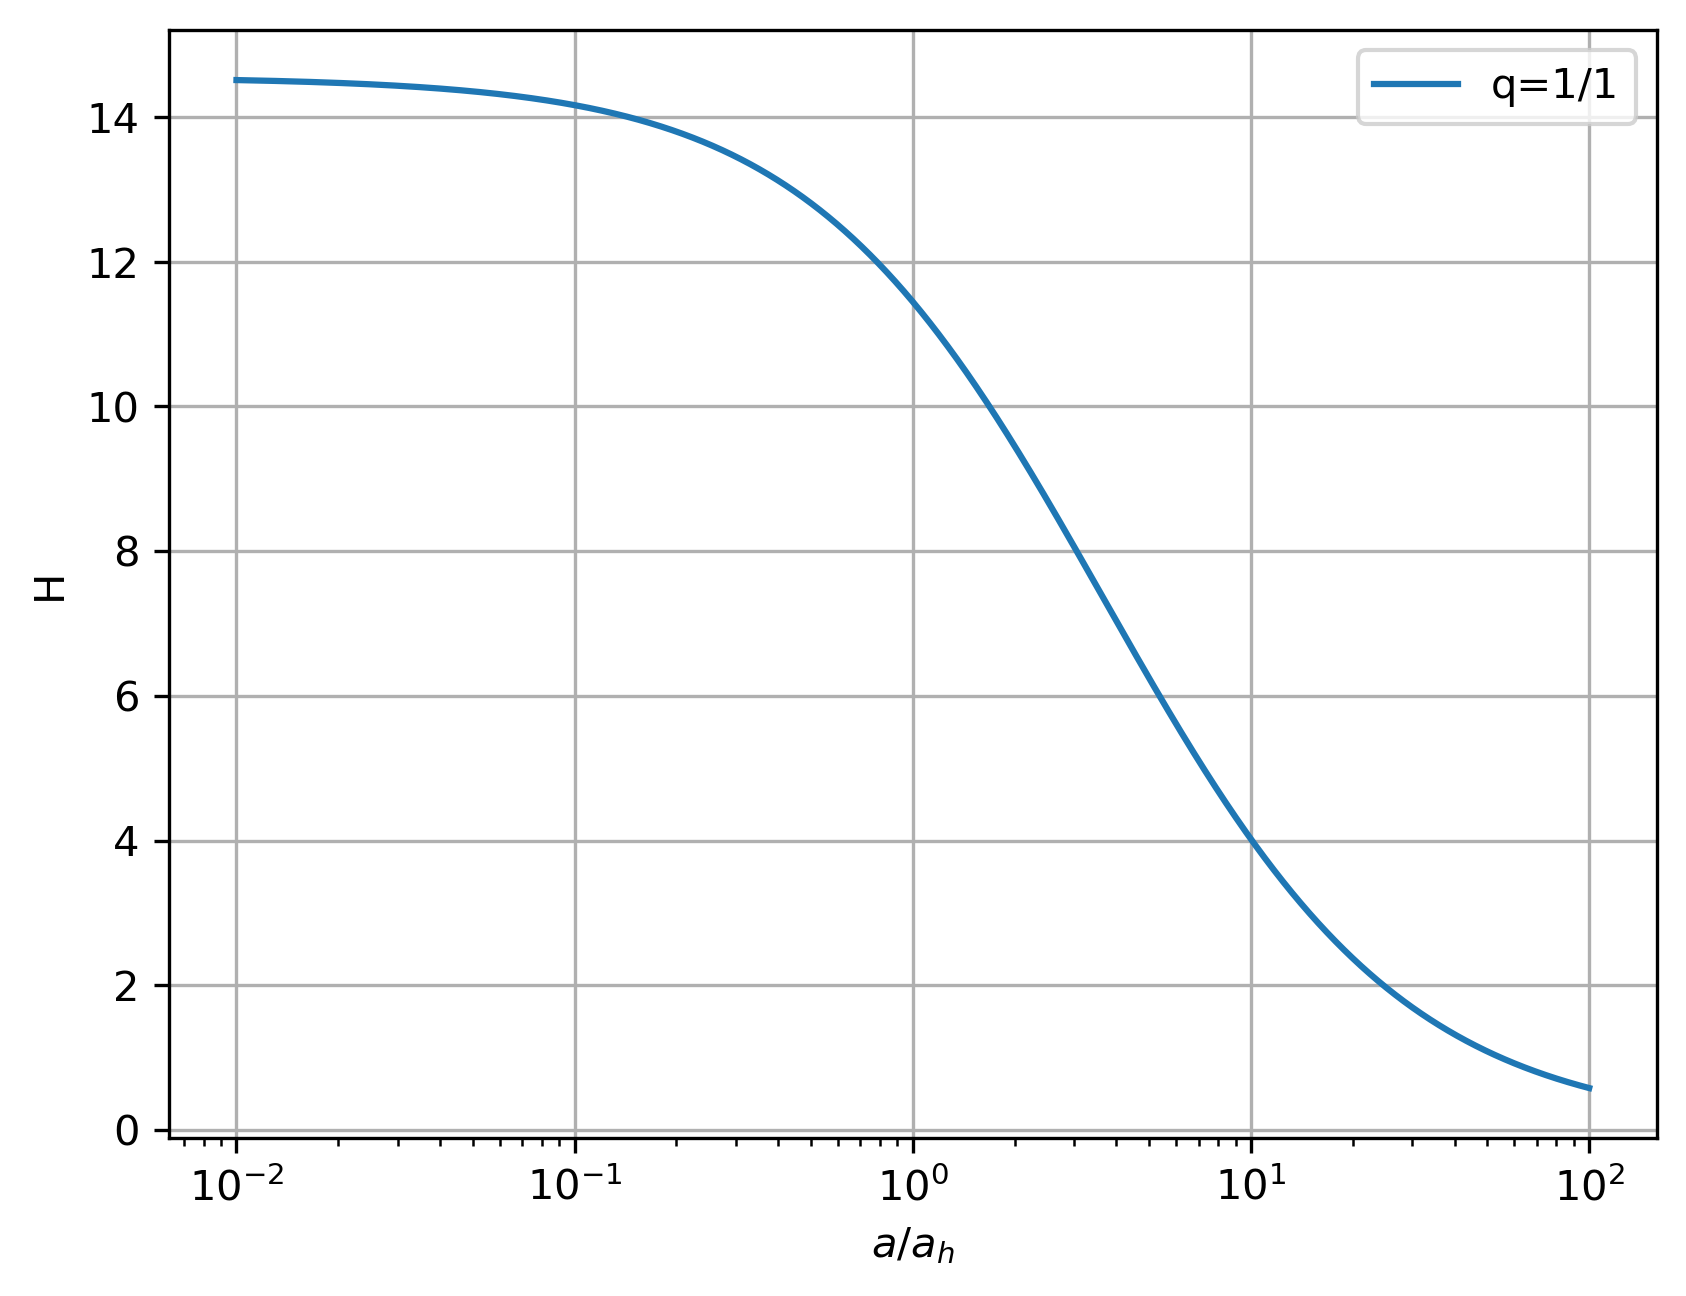
\includegraphics[width=0.5\linewidth]{H_vs_a.png}
    \caption{H as a function of $a$ expressed in $a_h$ units.}
    \label{Sesana comparison H plot}
\end{figure}






\begin{figure}[H]
    \centering
    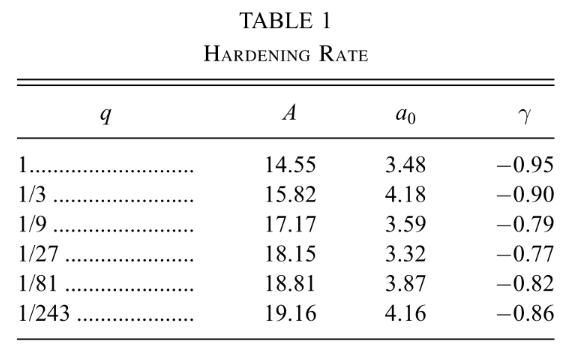
\includegraphics[width=0.5\linewidth]{Sesana_2006_Table_1.png}
    \caption{Note: $a_0$ is given in $a_h$ units.}
    \label{Sesana_2006_Table_1}
\end{figure}
Similarly, by interpolation over the eccentricty grid of Table 3 \cite{Sesana_2006} parameters, it is obtained
 \begin{equation}\label{Sesana_2006 K fit}
    K=A(1+a/a_0)^\gamma+B.
\end{equation}

\begin{figure}[H]
    \centering
    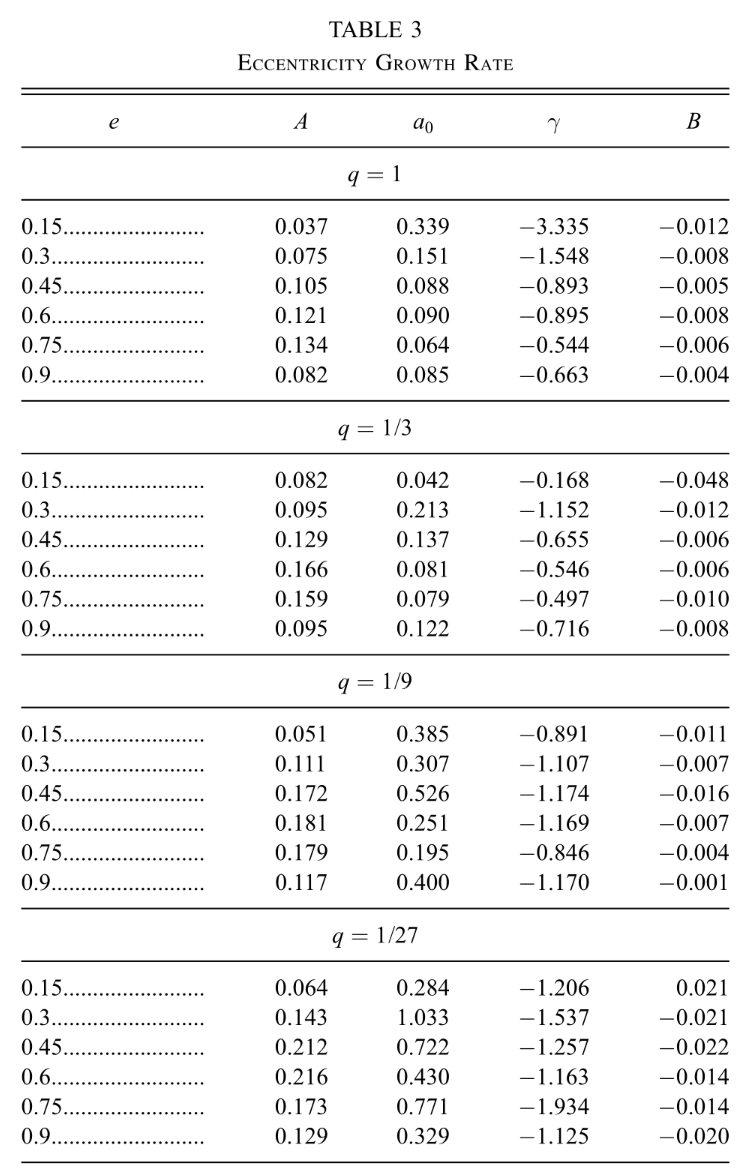
\includegraphics[width=0.5\linewidth]{Sesana_2006_Table_3.png}
    \caption{Note: $a_0$ is given in $a_h$ units.}
    \label{Sesana_2006_Table_3}
\end{figure}

Figure \ref{A of K fit Sesana comparison},\ref{a_0 of K fit Sesana comparison}, \ref{gamma of K fit Sesana comparison} and \ref{B of K fit Sesana comparison} report the results of this mathematical operation.


\begin{figure}[H]
    \centering
    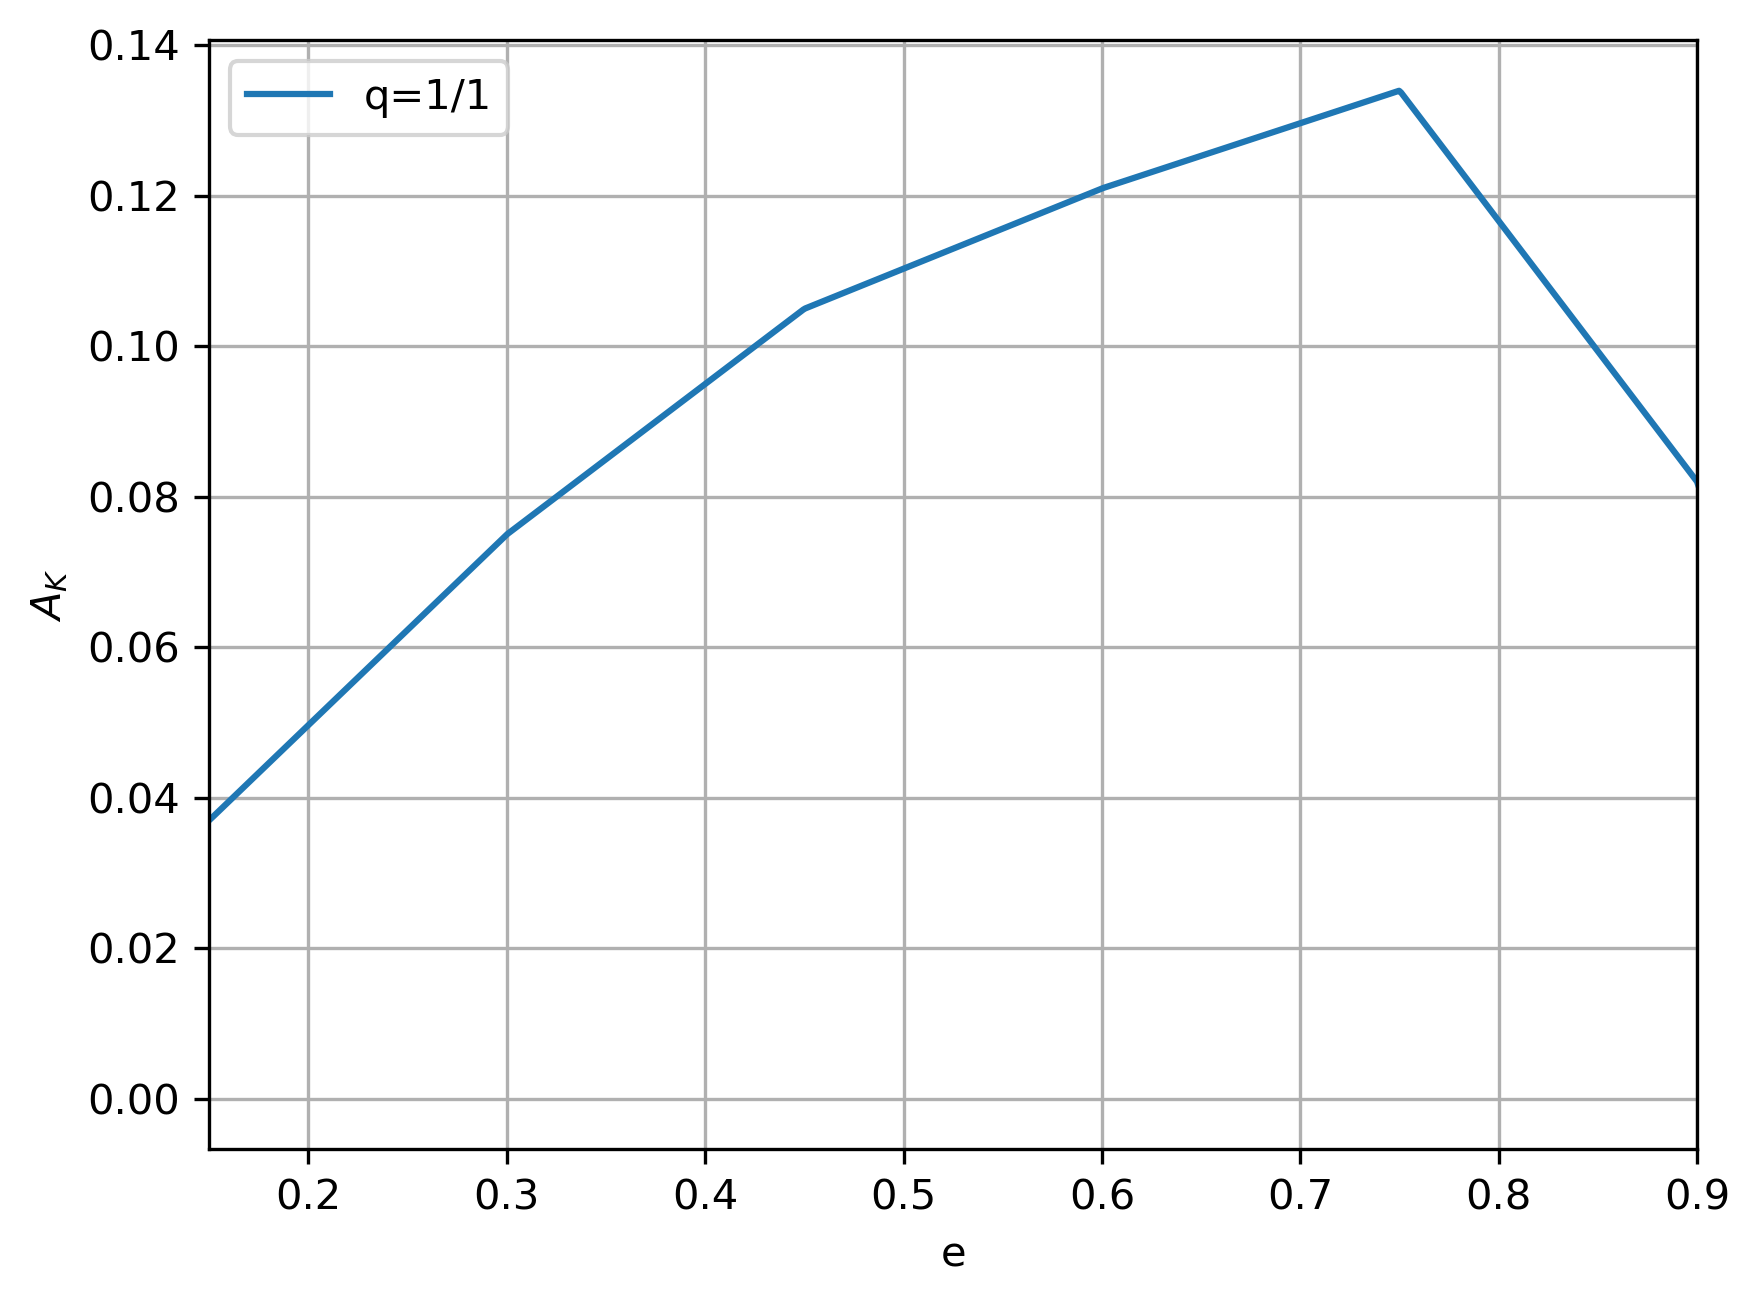
\includegraphics[width=0.5\linewidth]{A_K_vs_e.png}
    \caption{$A$ as a function of $e$ derived by interpolation of grid points.}
    \label{A of K fit Sesana comparison}
\end{figure}


\begin{figure}[H]
    \centering
    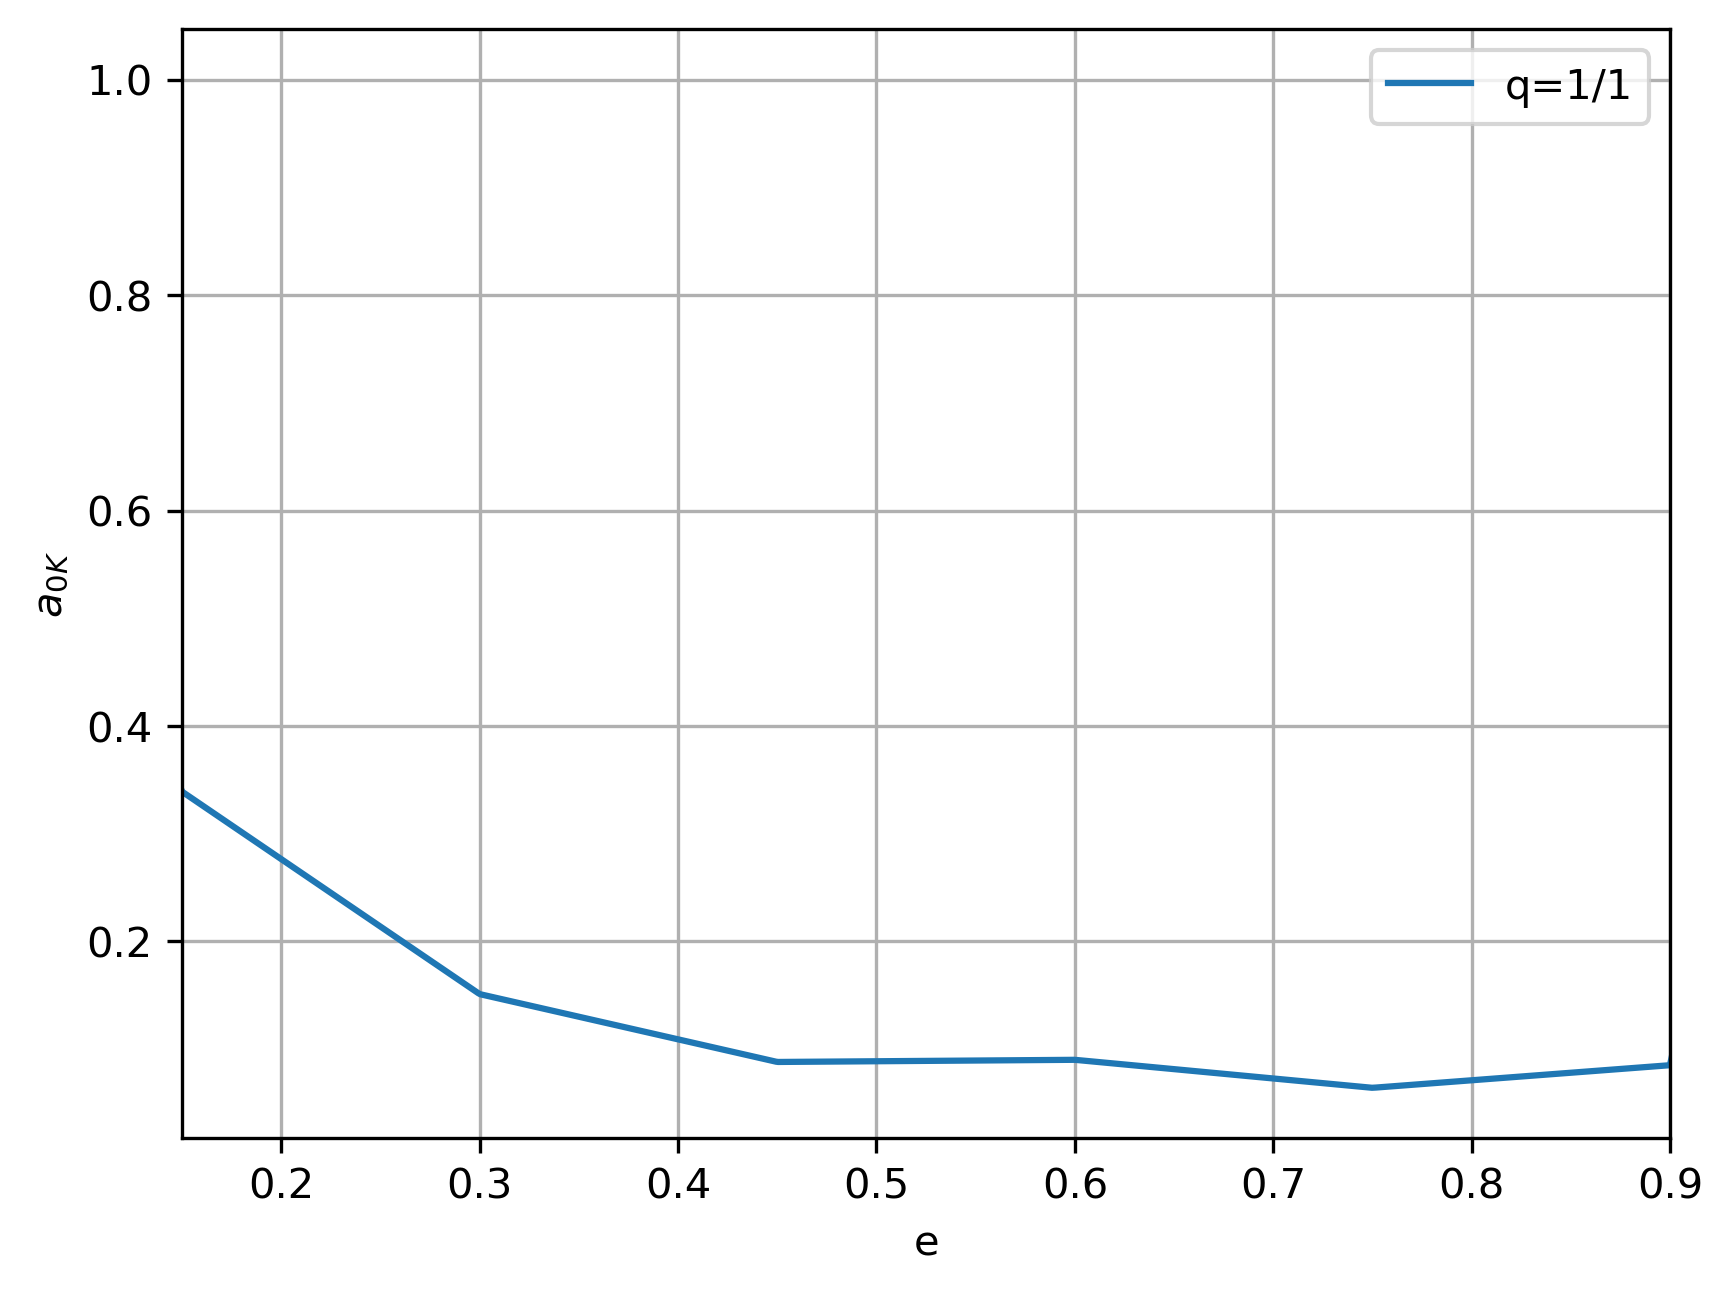
\includegraphics[width=0.5\linewidth]{a0_K_vs_e.png}
    \caption{$A$ as a function of $e$ derived by interpolation of grid points.}
    \label{a_0 of K fit Sesana comparison}
\end{figure}


\begin{figure}[H]
    \centering
    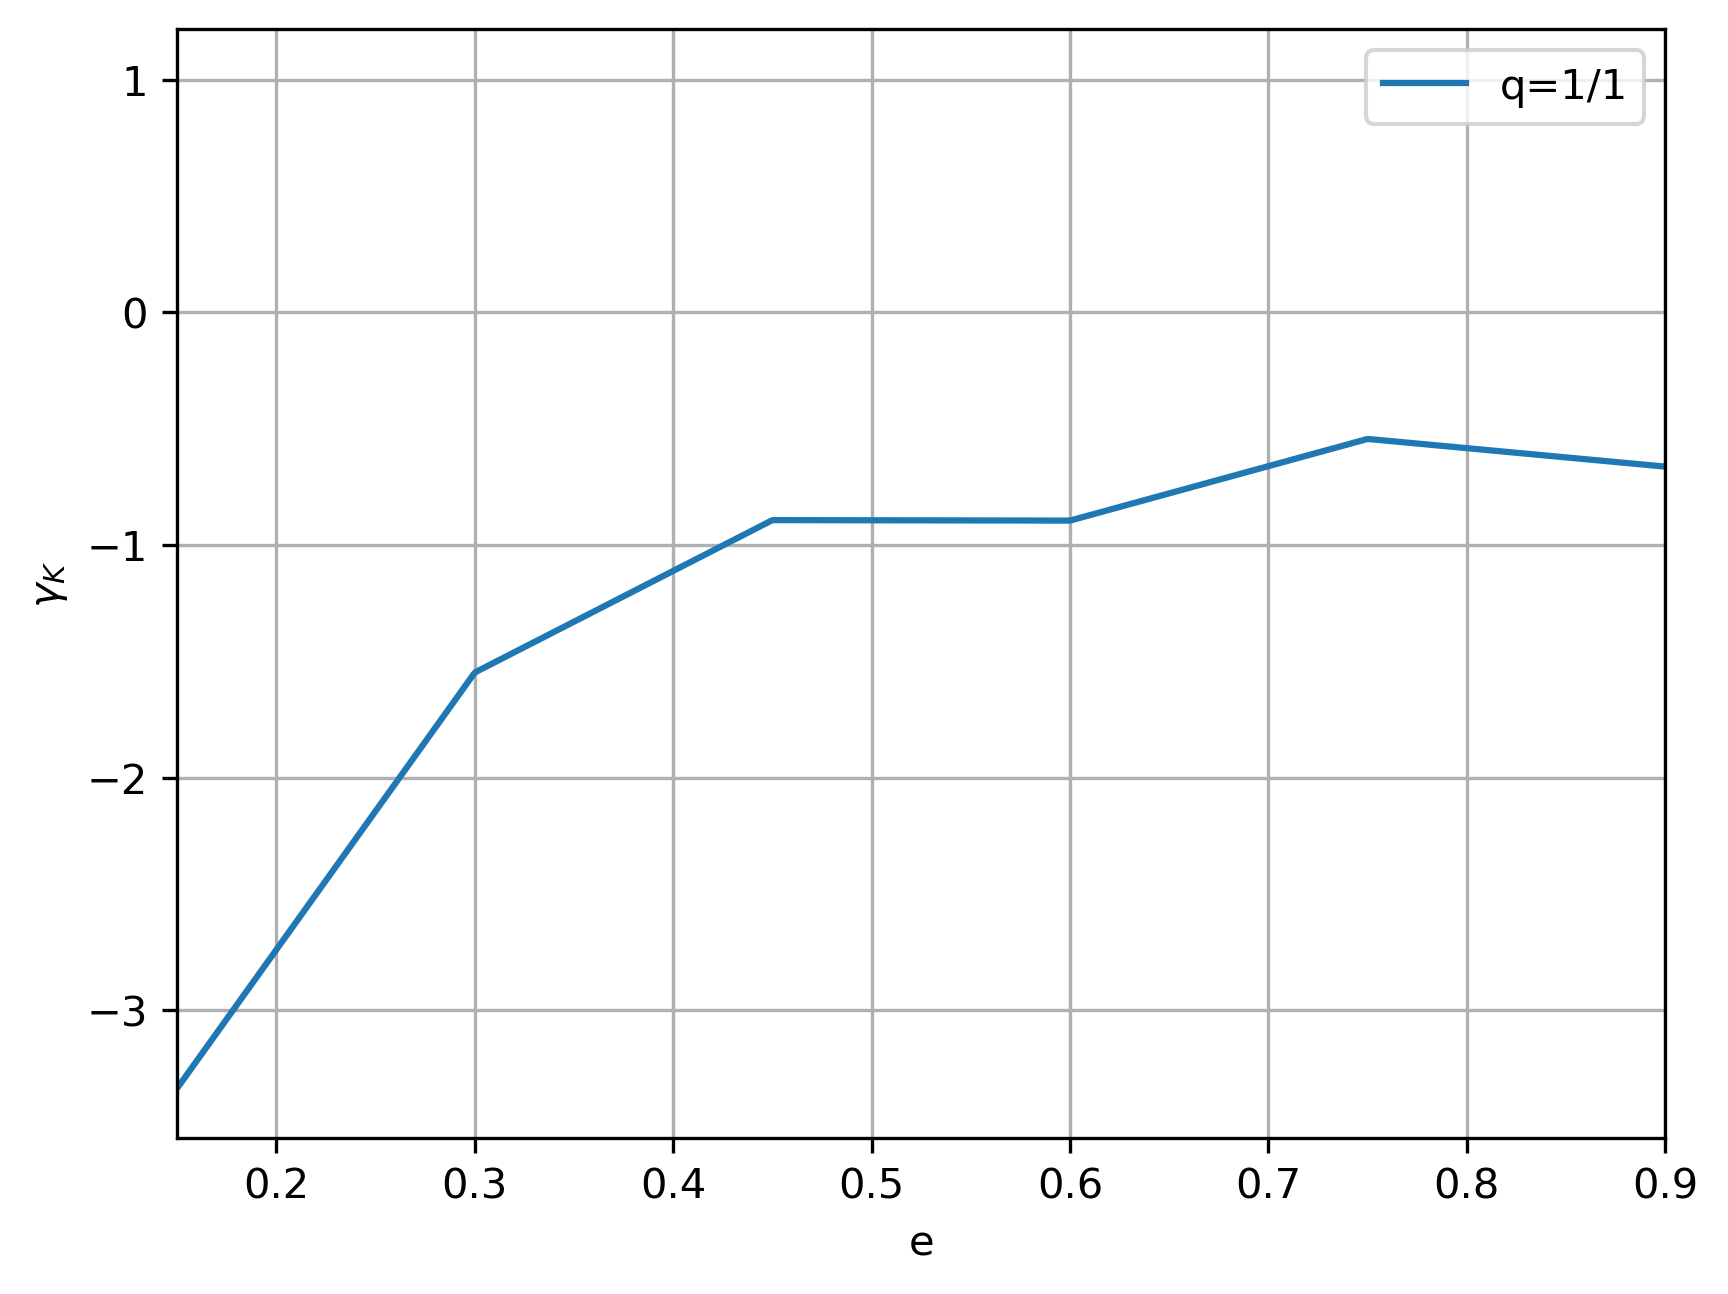
\includegraphics[width=0.5\linewidth]{gamma_K_vs_e.png}
    \caption{$\gamma$ as a function of $e$ derived by interpolation of grid points.}
    \label{gamma of K fit Sesana comparison}
\end{figure}






\begin{figure}[H]
    \centering
    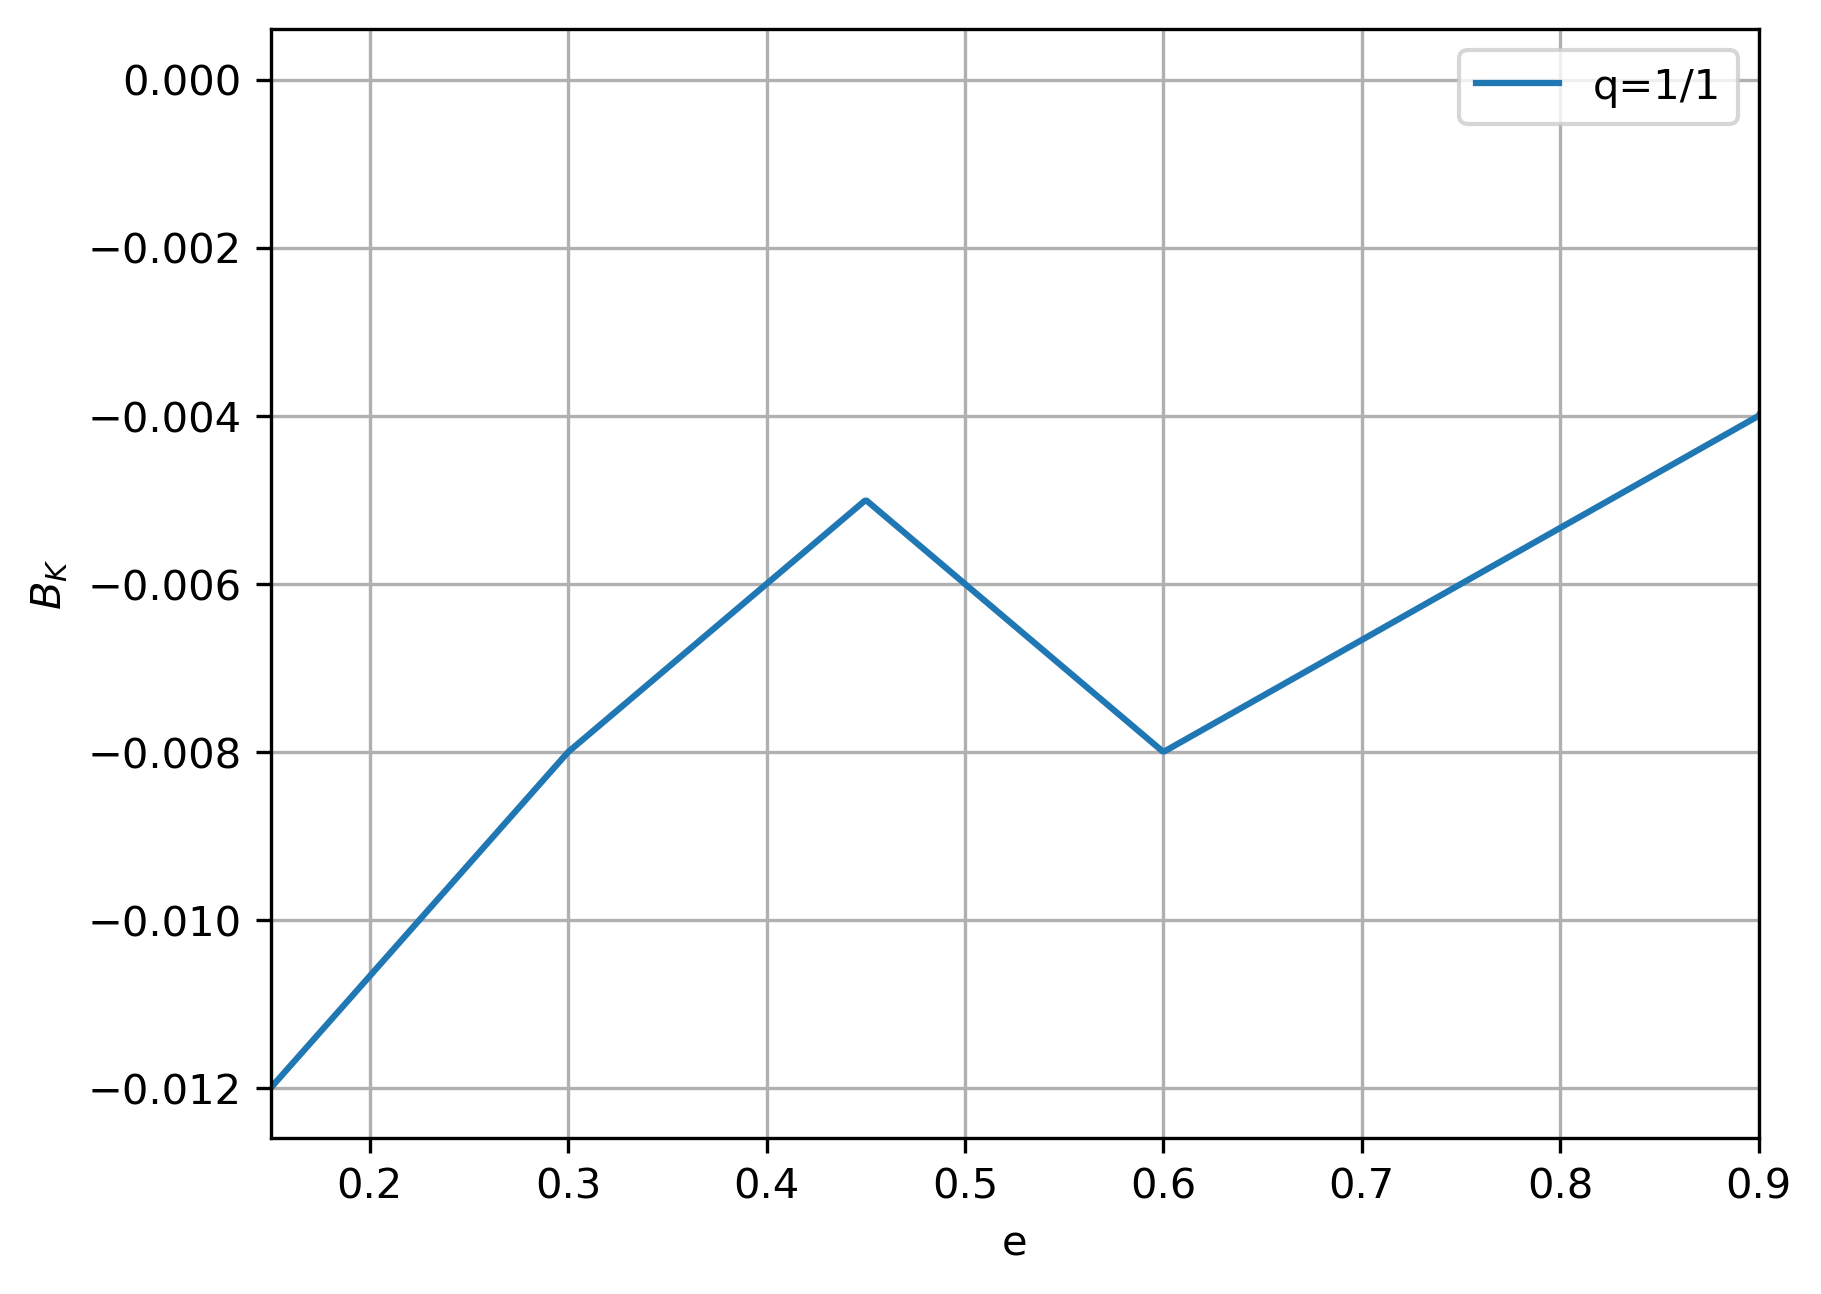
\includegraphics[width=0.5\linewidth]{B_K_vs_e.png}
    \caption{$B$ as a function of $e$ derived by interpolation of grid points.}
    \label{B of K fit Sesana comparison}
\end{figure}

Therefore, at odds with $H$, $K$ is a function of $(a,e)$; we list below the plots of the 1-D functions $K(a)=K(a,e_0)$ and $K(e)=K(a_h,e)$.


\begin{figure}[H]
    \centering
    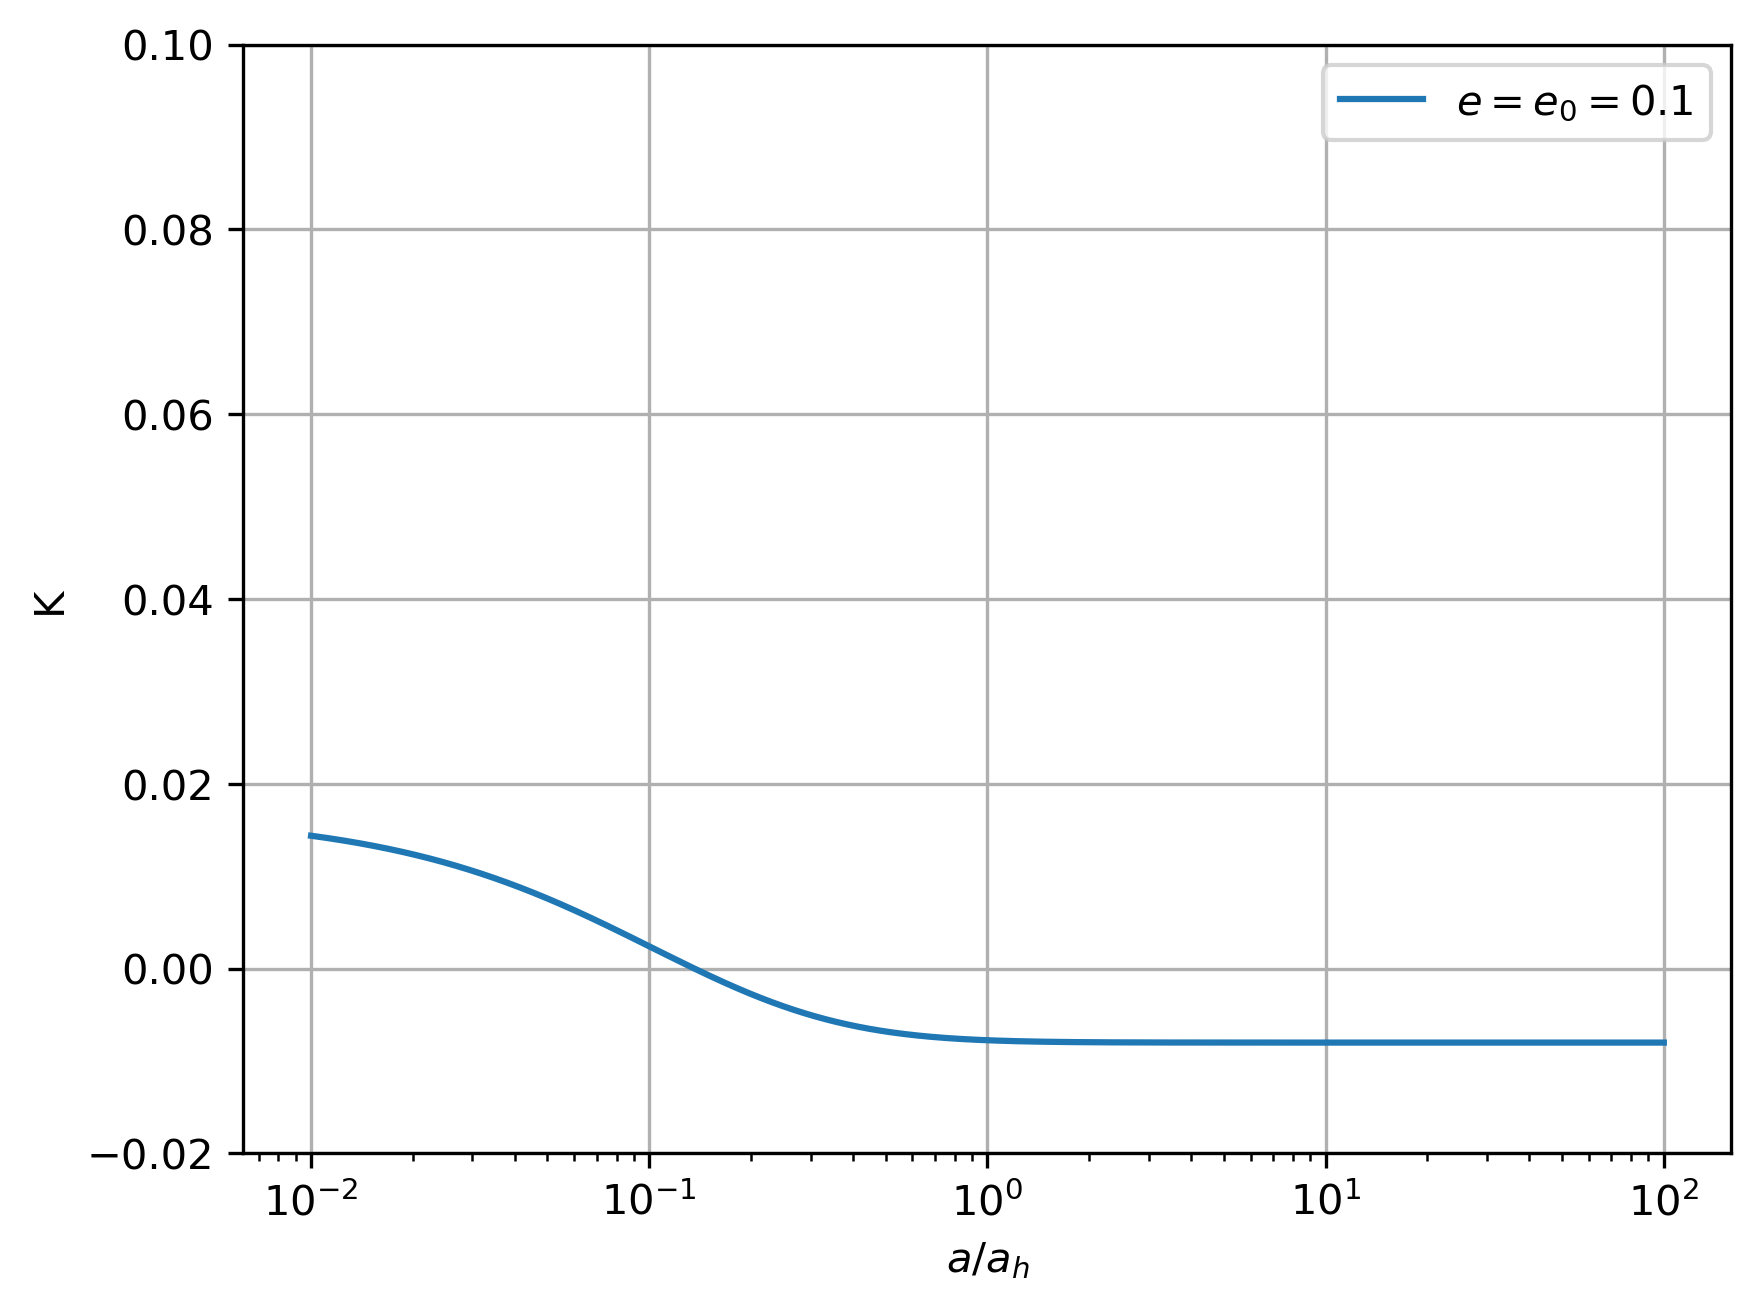
\includegraphics[width=0.5\linewidth]{K_vs_a.png}
    \caption{}
    \label{K vs a Sesana comparison}
\end{figure}


\begin{figure}[H]
    \centering
    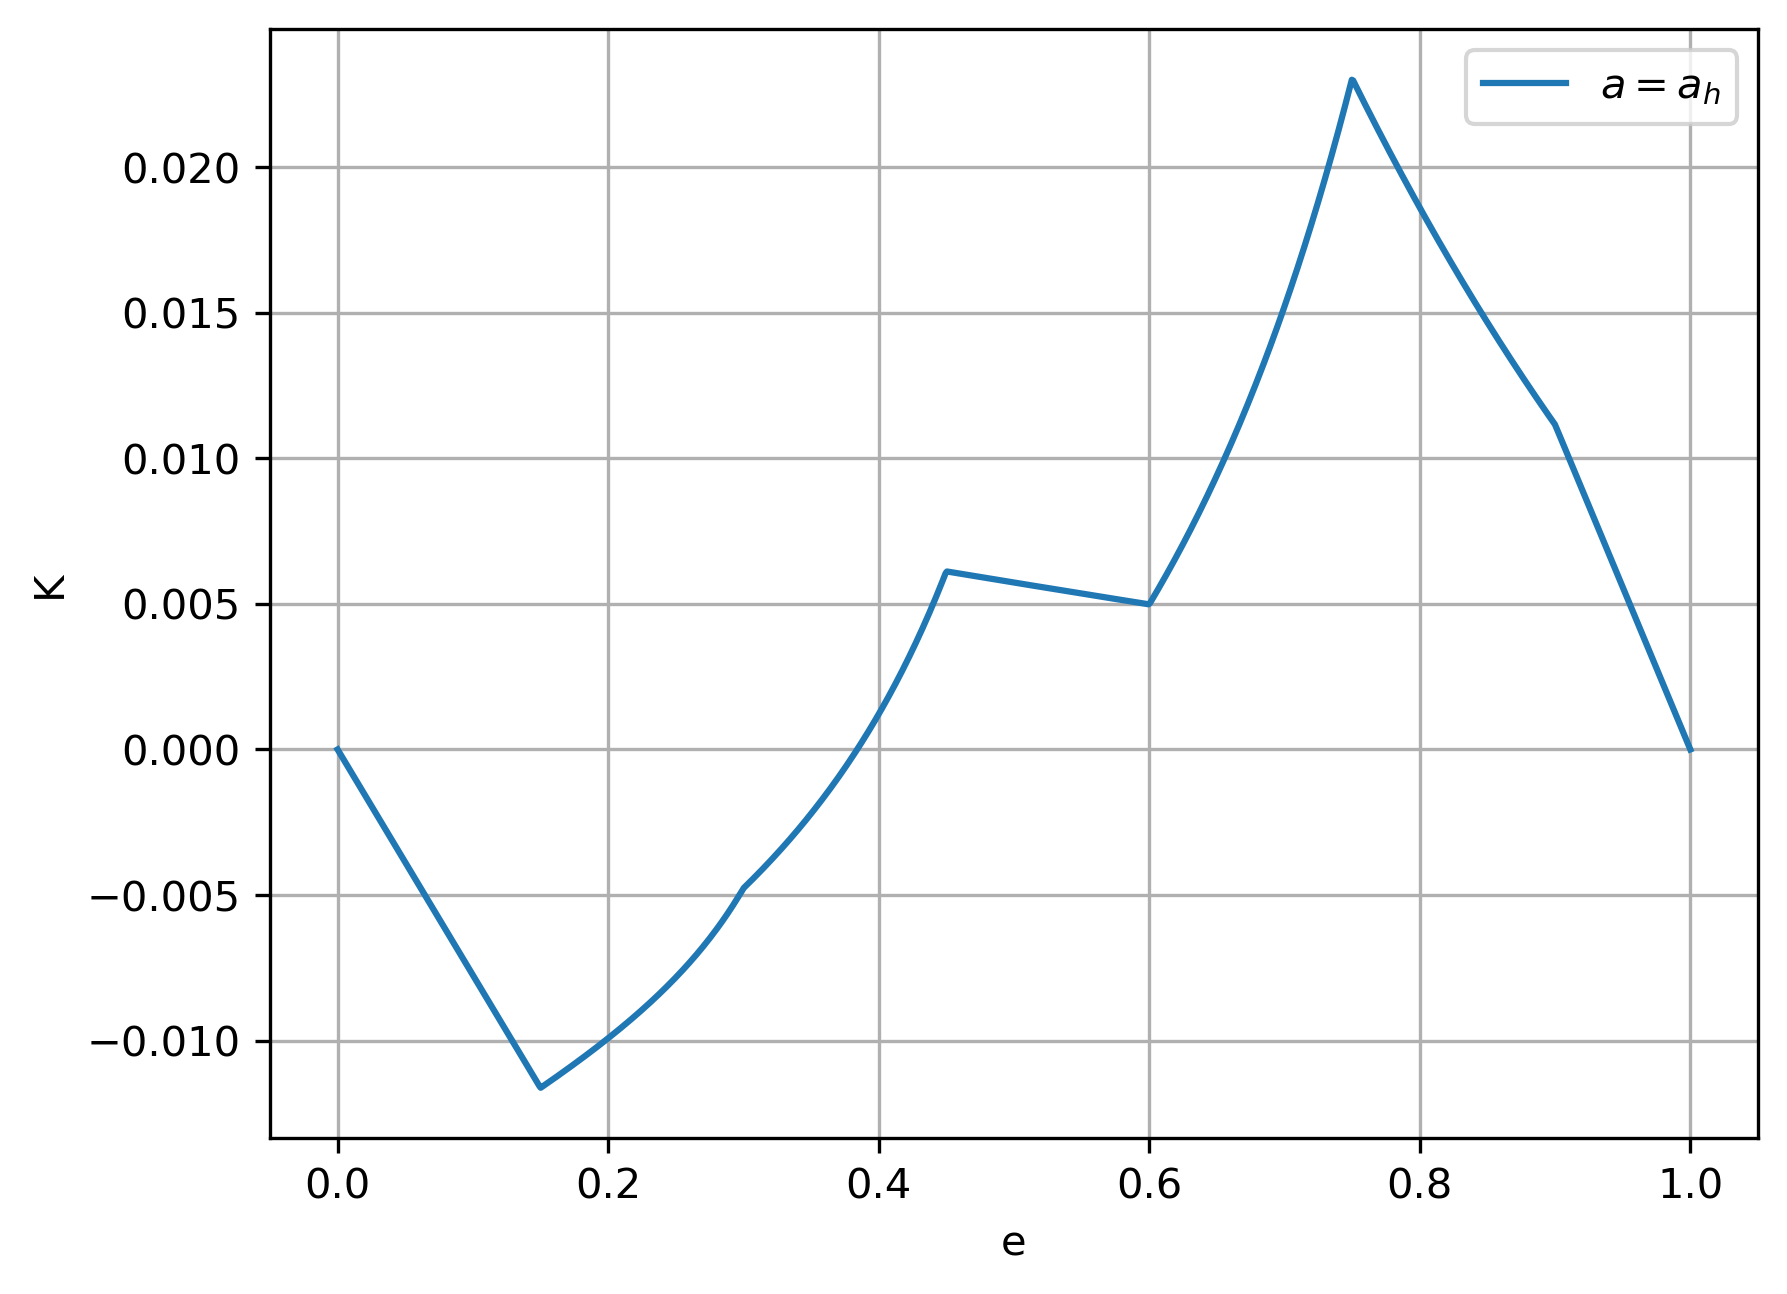
\includegraphics[width=0.5\linewidth]{K_vs_e.png}
    \caption{}
    \label{K vs e Sesana comparison}
\end{figure}
We anticipate that Equations (\ref{Sesana_2010 da/dt TOT}) and (\ref{Sesana_2010 de/dt TOT}) will be integrated with the help of RK(4) and $dK/de$ is needed as well; Figure \ref{dK/de vs e Sesana comparison} depicts the step-like function.

\begin{figure}[H]
    \centering
    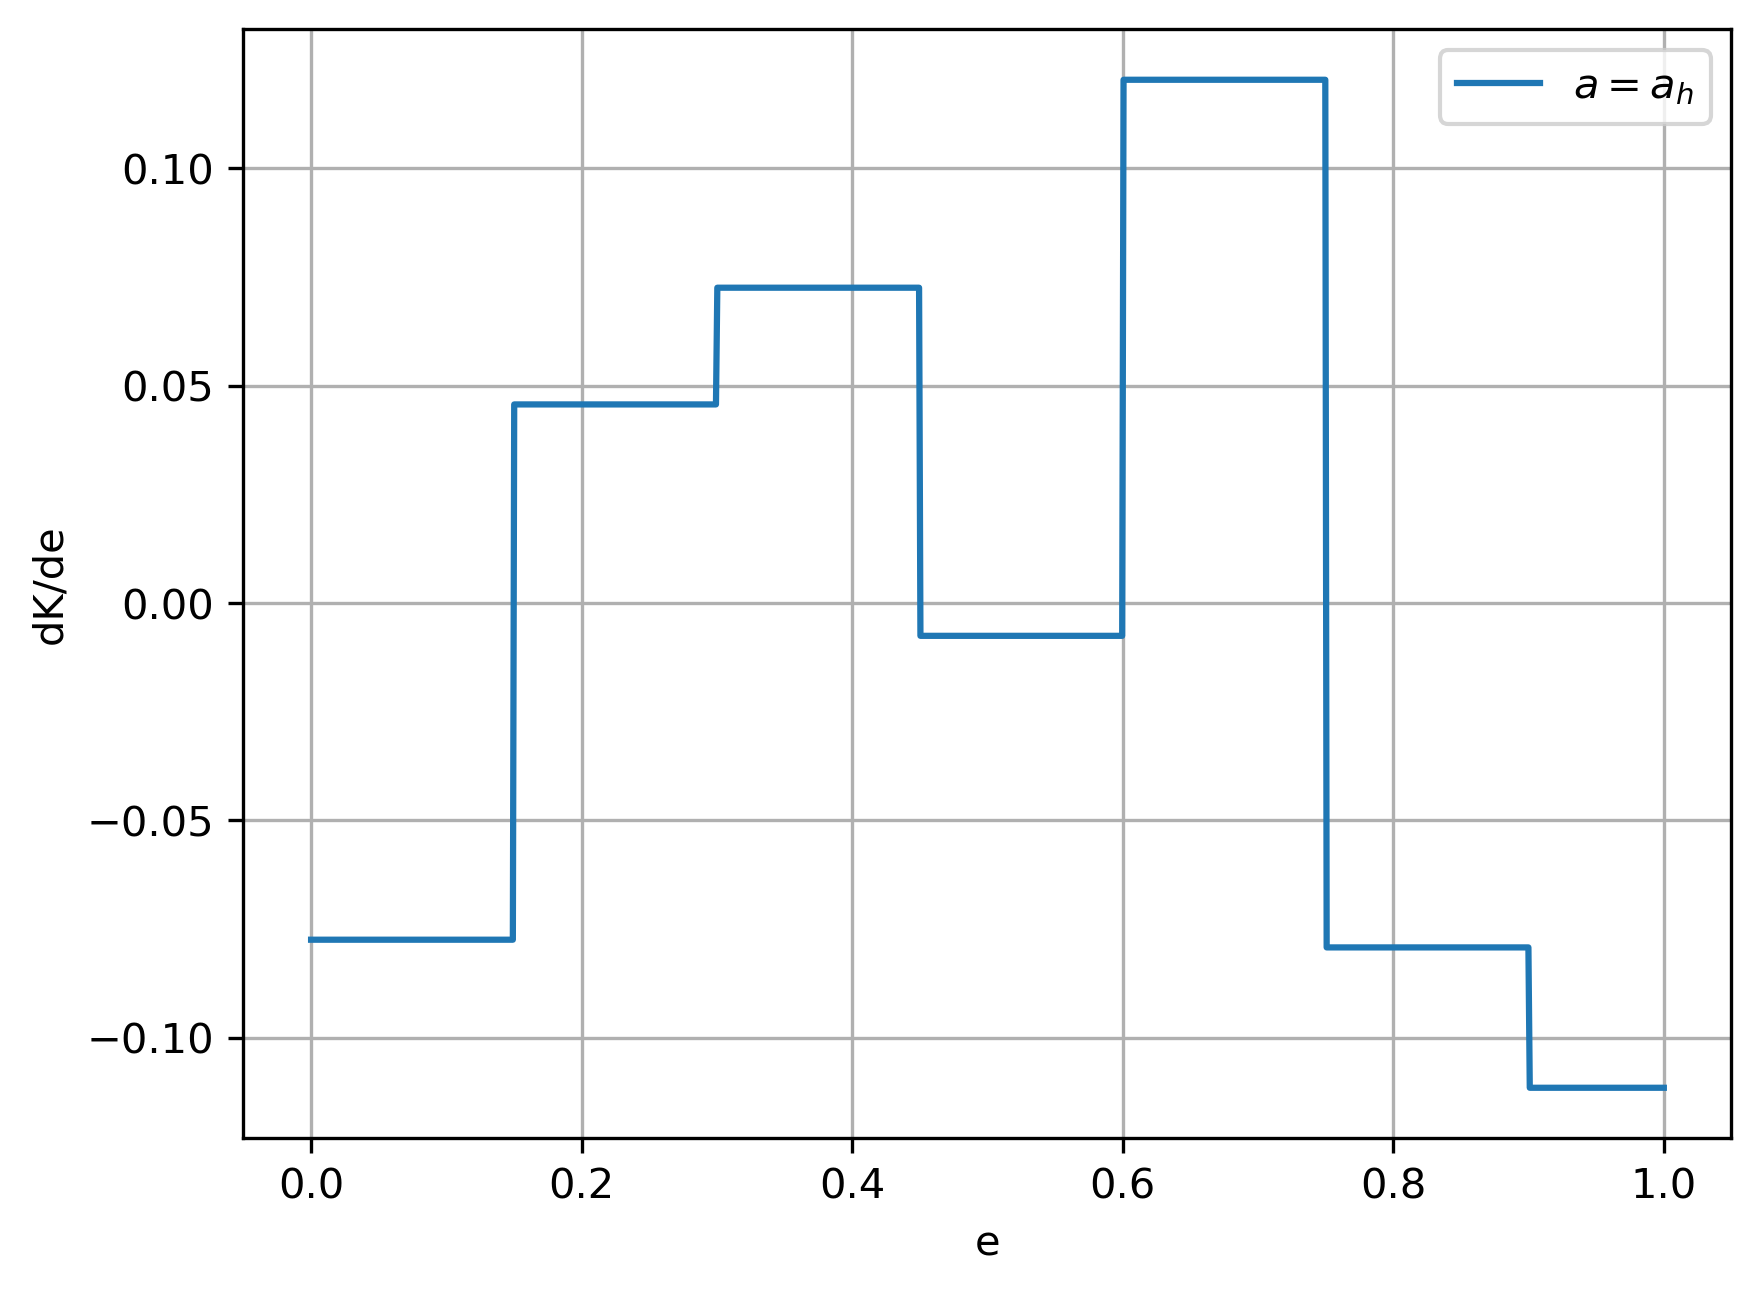
\includegraphics[width=0.5\linewidth]{dK_de_vs_e.png}
    \caption{}
    \label{dK/de vs e Sesana comparison}
\end{figure}
The time step is adjusted at each iteration according to the prescription
\begin{equation}
    \Delta t \le  min\left \{\frac{2.79}{|\lambda_i|}\right\} \qquad \forall i=1,N
\end{equation}
where $\lambda_i$ are the Jacobian $\mathbf{J}$ eigenvalues. The elements of this matrix are:
\begin{equation}\label{J_11 of Sesana comparison}
    J_{11}=\left. \frac{da}{dt}\right|_u\left(\frac{2}{a}+\frac{\gamma}{a+a_0a_h}\right)-\left.\frac{da}{dt}\right|_{gw}\left(\frac{3}{a}\right)
\end{equation}


\begin{equation}\label{J_12 of Sesana comparison}
    J_{12}=\left. \frac{da}{dt}\right|_{GW}\left(\frac{{7e}}{1-e^2}+\frac{73e/12+37e^3/24}{1+73e^2/24+37e^4/96}\right)
\end{equation}





\begin{equation}\label{J_21 of Sesana comparison}
    J_{21}=\left.\frac{de}{dt}\right|_u\left(\frac{1}{a}+\frac{\gamma_H}{a+a_{0,H}a_h}+\frac{\gamma_K}{a+a_{0,K}a_h}\right)-\left.\frac{de}{dt}\right|_{GW}\left(\frac{4}{a}\right)
\end{equation}


\begin{equation}\label{J_22 of Sesana comparison}
    J_{22}=\left.\frac{de}{dt}\right|_u\left(\frac{\partial \ln{K}}{\partial e}\right)+\left.\frac{de}{dt}\right|_{GW}\left(\frac{5e}{1-e^2}+\frac{1+363e^2/304}{e+121e^3/304}\right)
\end{equation}


In order to compare Sesana predictions with our model we set $(t_0,a_0,e_0)$ for the unbound phase to be effective and selecting these values directely from Sesana plot: $(t_0,a_0,e_0)=(12Myr,0.05\cdot a_0, 0.131 )$.


\begin{figure}[H]
    \centering
    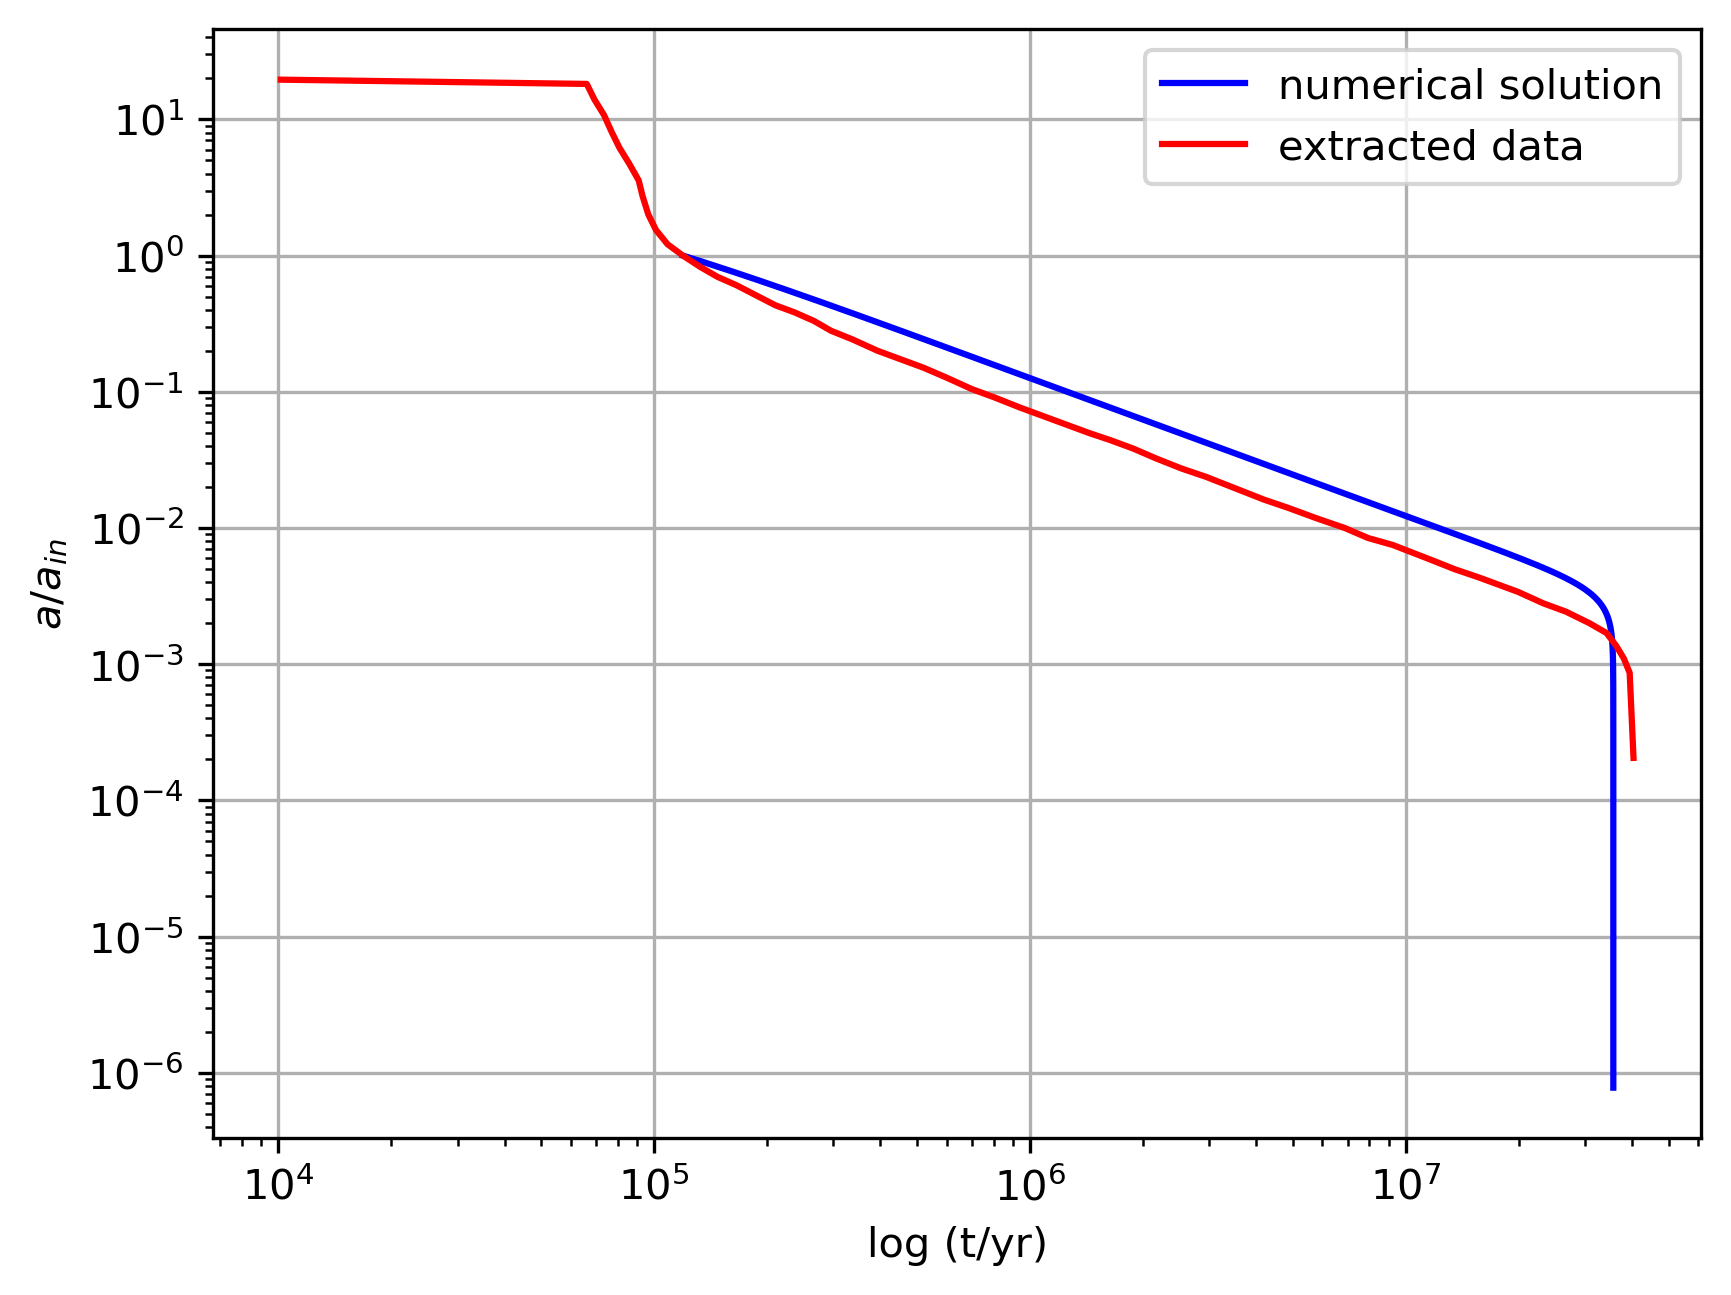
\includegraphics[width=0.5\linewidth]{a_vs_t_check.png}
    \caption{}
    \label{a vs t Sesana comparison}
\end{figure}



\begin{figure}[H]
    \centering
    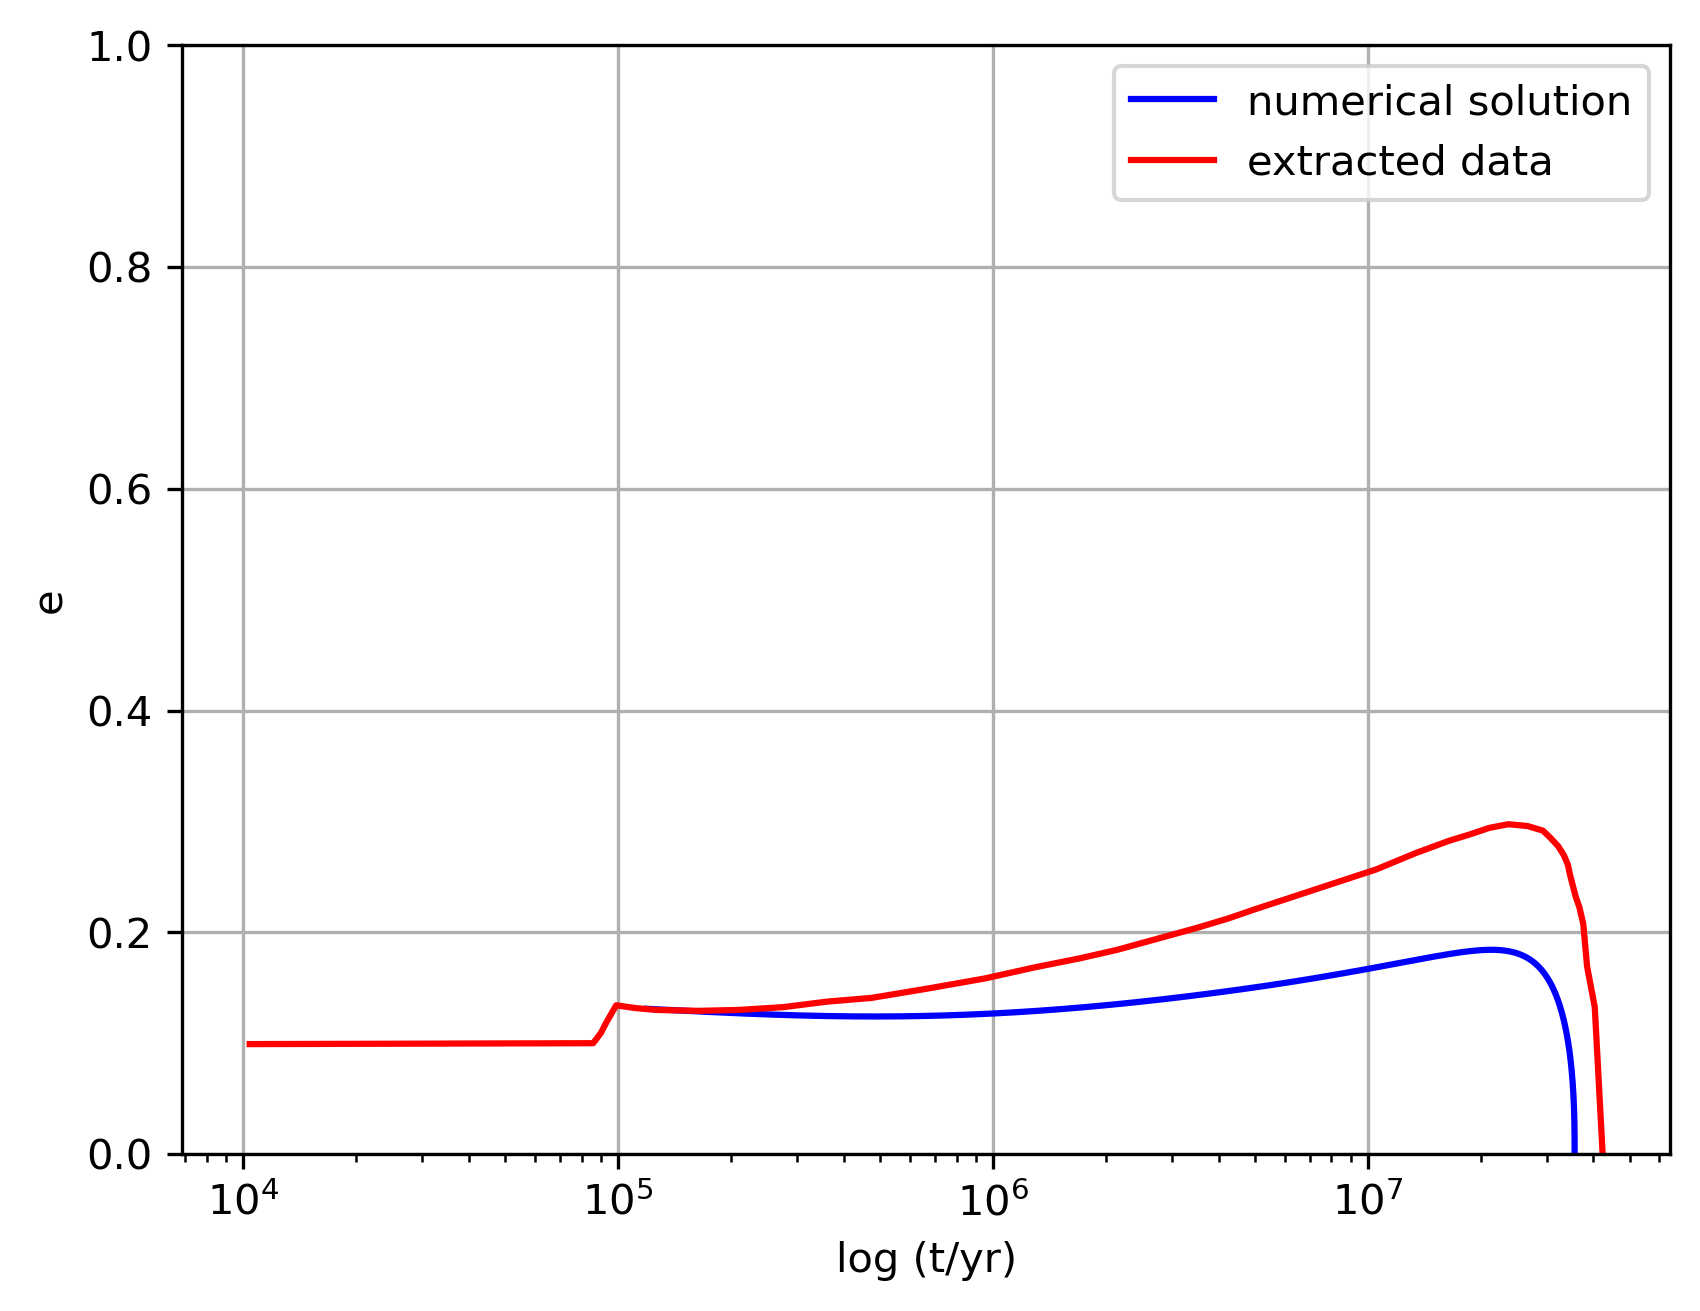
\includegraphics[width=0.5\linewidth]{e_vs_t_check.png}
    \caption{}
    \label{e vs t Sesana comparison}
\end{figure}

Figure \ref{a vs t Sesana comparison} and \ref{e vs t Sesana comparison} indicate a good agreement between our model and Sesana one. In the first plot $a$ decreases more slowly than Sesana prediction as we are negletting the bound cusp erosion contribute, which hardens the binary even when the unbond phase takes over at $\sim a_h$. On the other hand eccentricity reaches a lower peak compared to the reference model because of bound cusp erosion leads to $e$ growth as well.\\Furthermore, we test the feedback of the various shrinking mechanisms by assuming them working in isoletion, hence suppressing all the others.

Figure \ref{a_vs_t_UN} and \ref{e_vs_t_UN} refers to the evolution under the effect of slinghot of unbound stars; as the initial separation is below $a_h$ we can appreciate the expected linear decay of $a$ and the overall eccentricity growth. 
\begin{figure}[H]
    \centering
  \begin{minipage}[c]{0.45\textwidth}
    \centering
    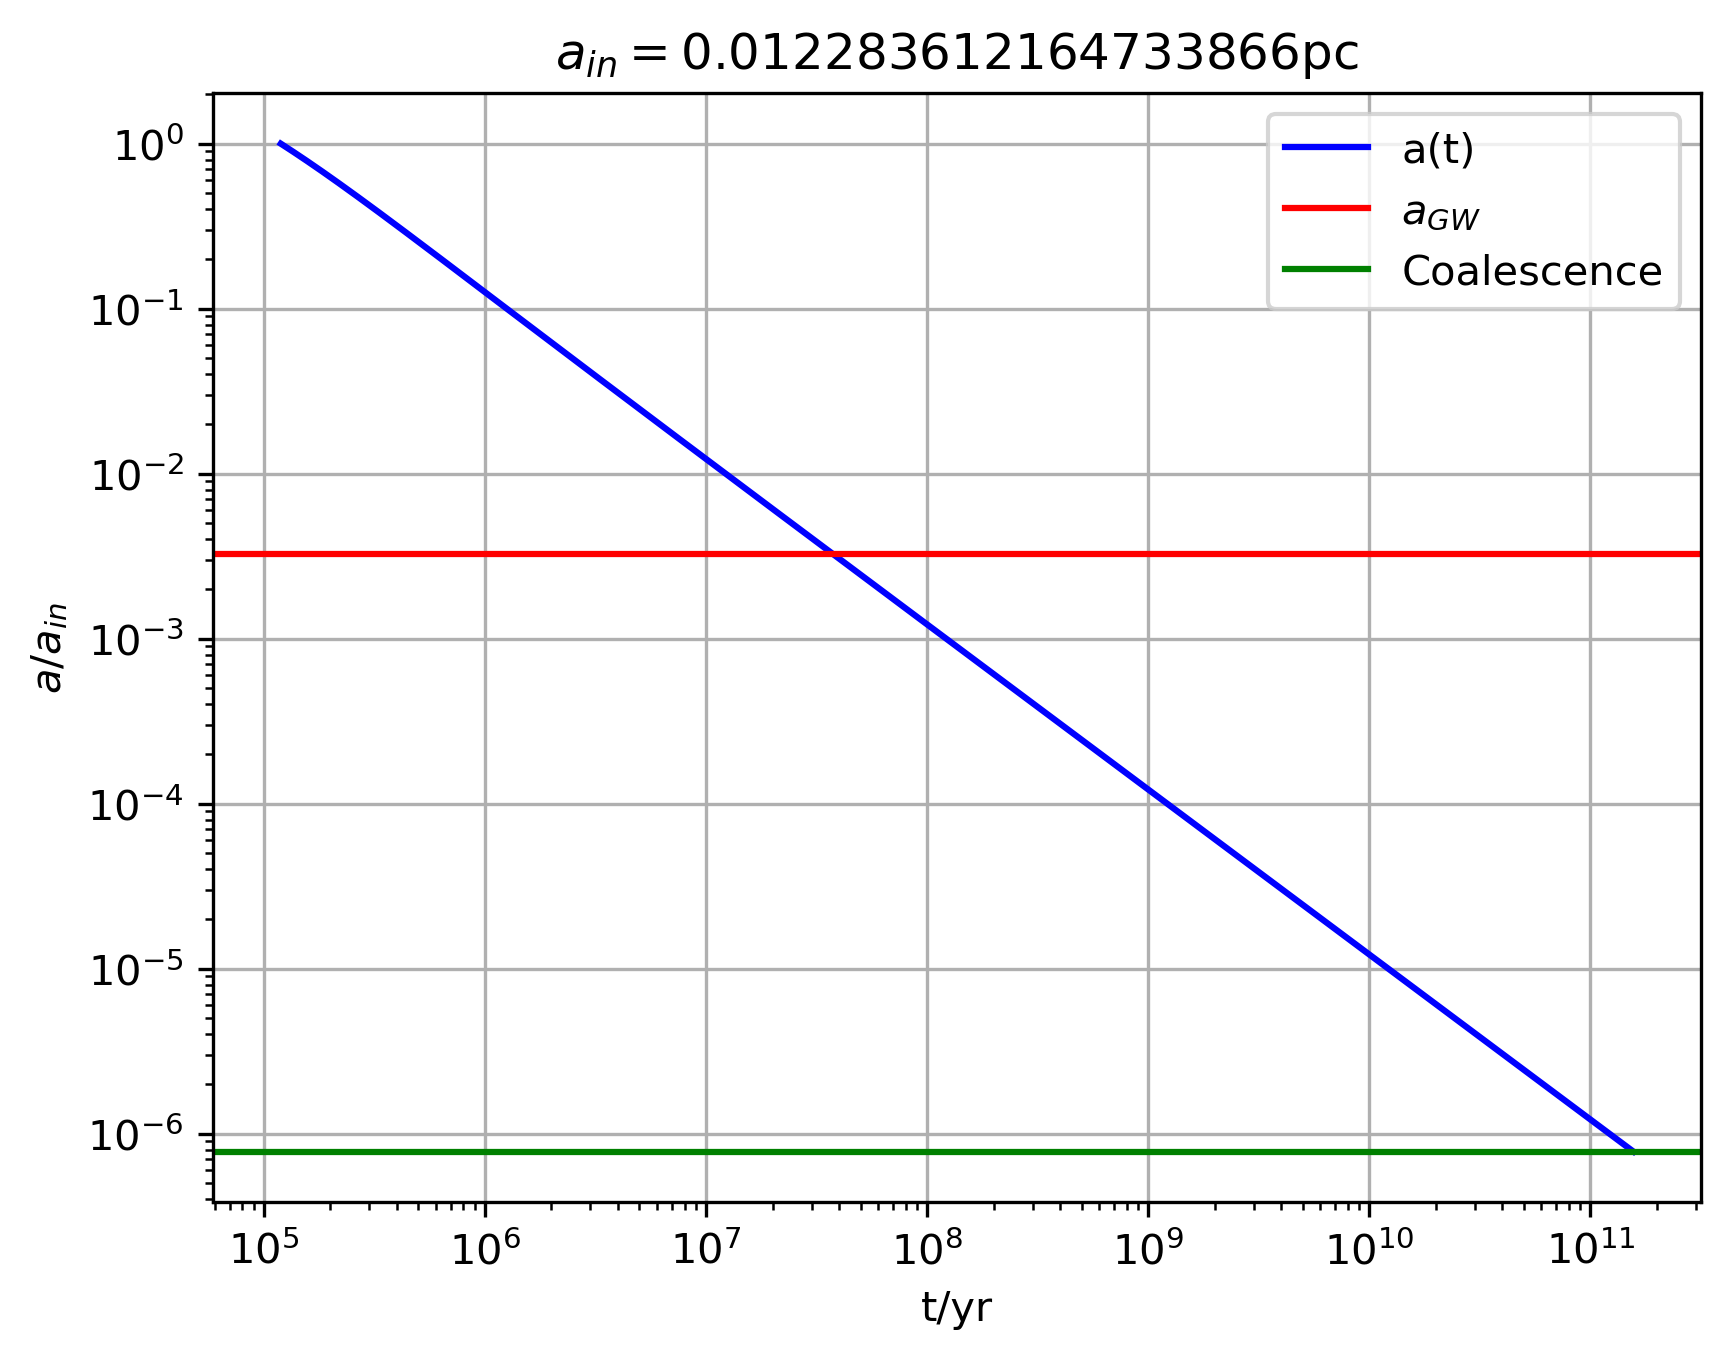
\includegraphics[height=5cm]{a_vs_t_UN.png}
    \caption{}
    \label{a_vs_t_UN}
    \vspace{2mm}
  \end{minipage}
  \hfill
  \begin{minipage}[c]{0.45\textwidth}
    \centering
    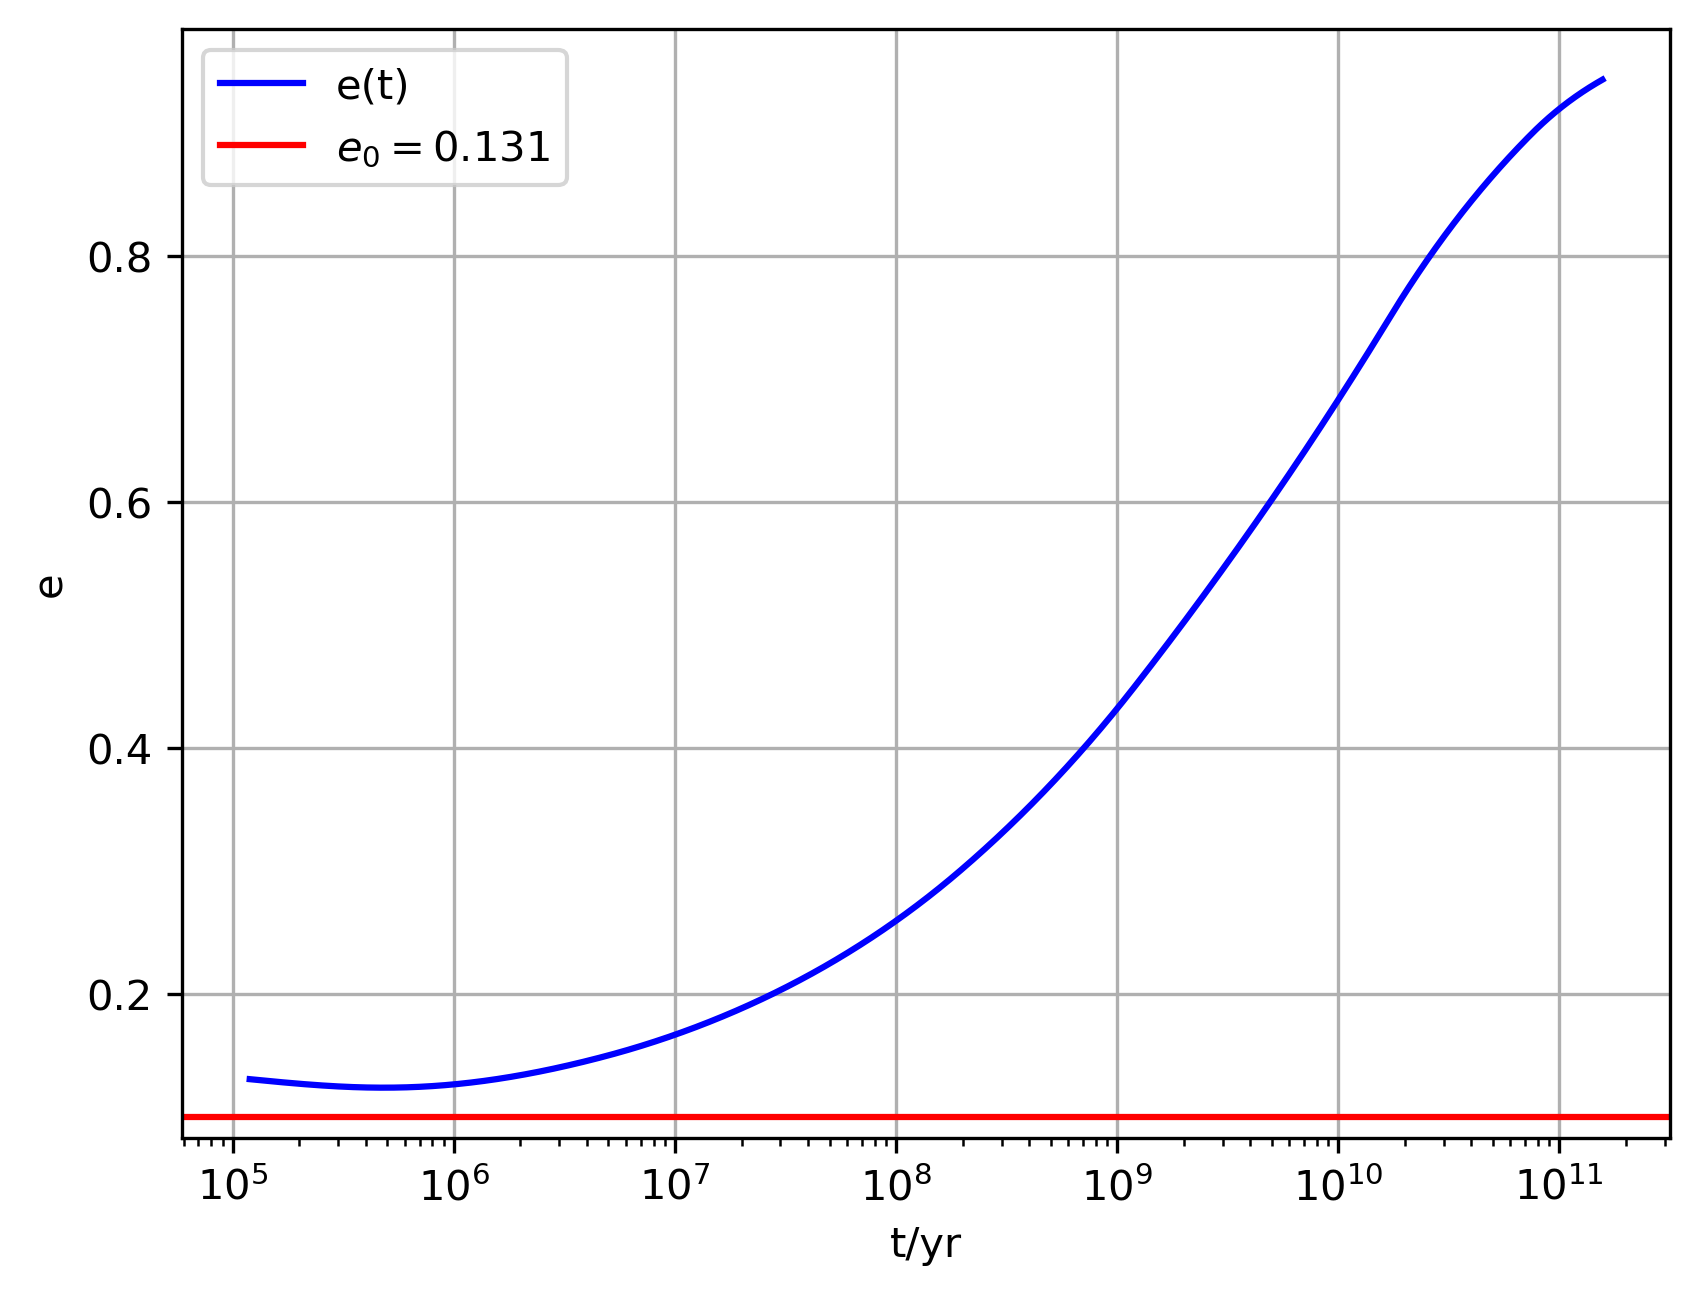
\includegraphics[height=5cm]{e_vs_t_UN.png}
    \caption{}
    \label{e_vs_t_UN}
    \vspace{2mm}
  \end{minipage}
\end{figure}



Figure \ref{a_vs_t_GW} and \ref{e_vs_t_GW} refers to the evolution under GWs production; this becomes effective only at very close separation and causes both the fast binary coalescence once effective and binary circularization. The coalescence time agrees perfectly to the theoretical prediction of Equation \ref{t_coal Maggiore} 




\begin{figure}[H]
    \centering
  \begin{minipage}[c]{0.45\textwidth}
    \centering
    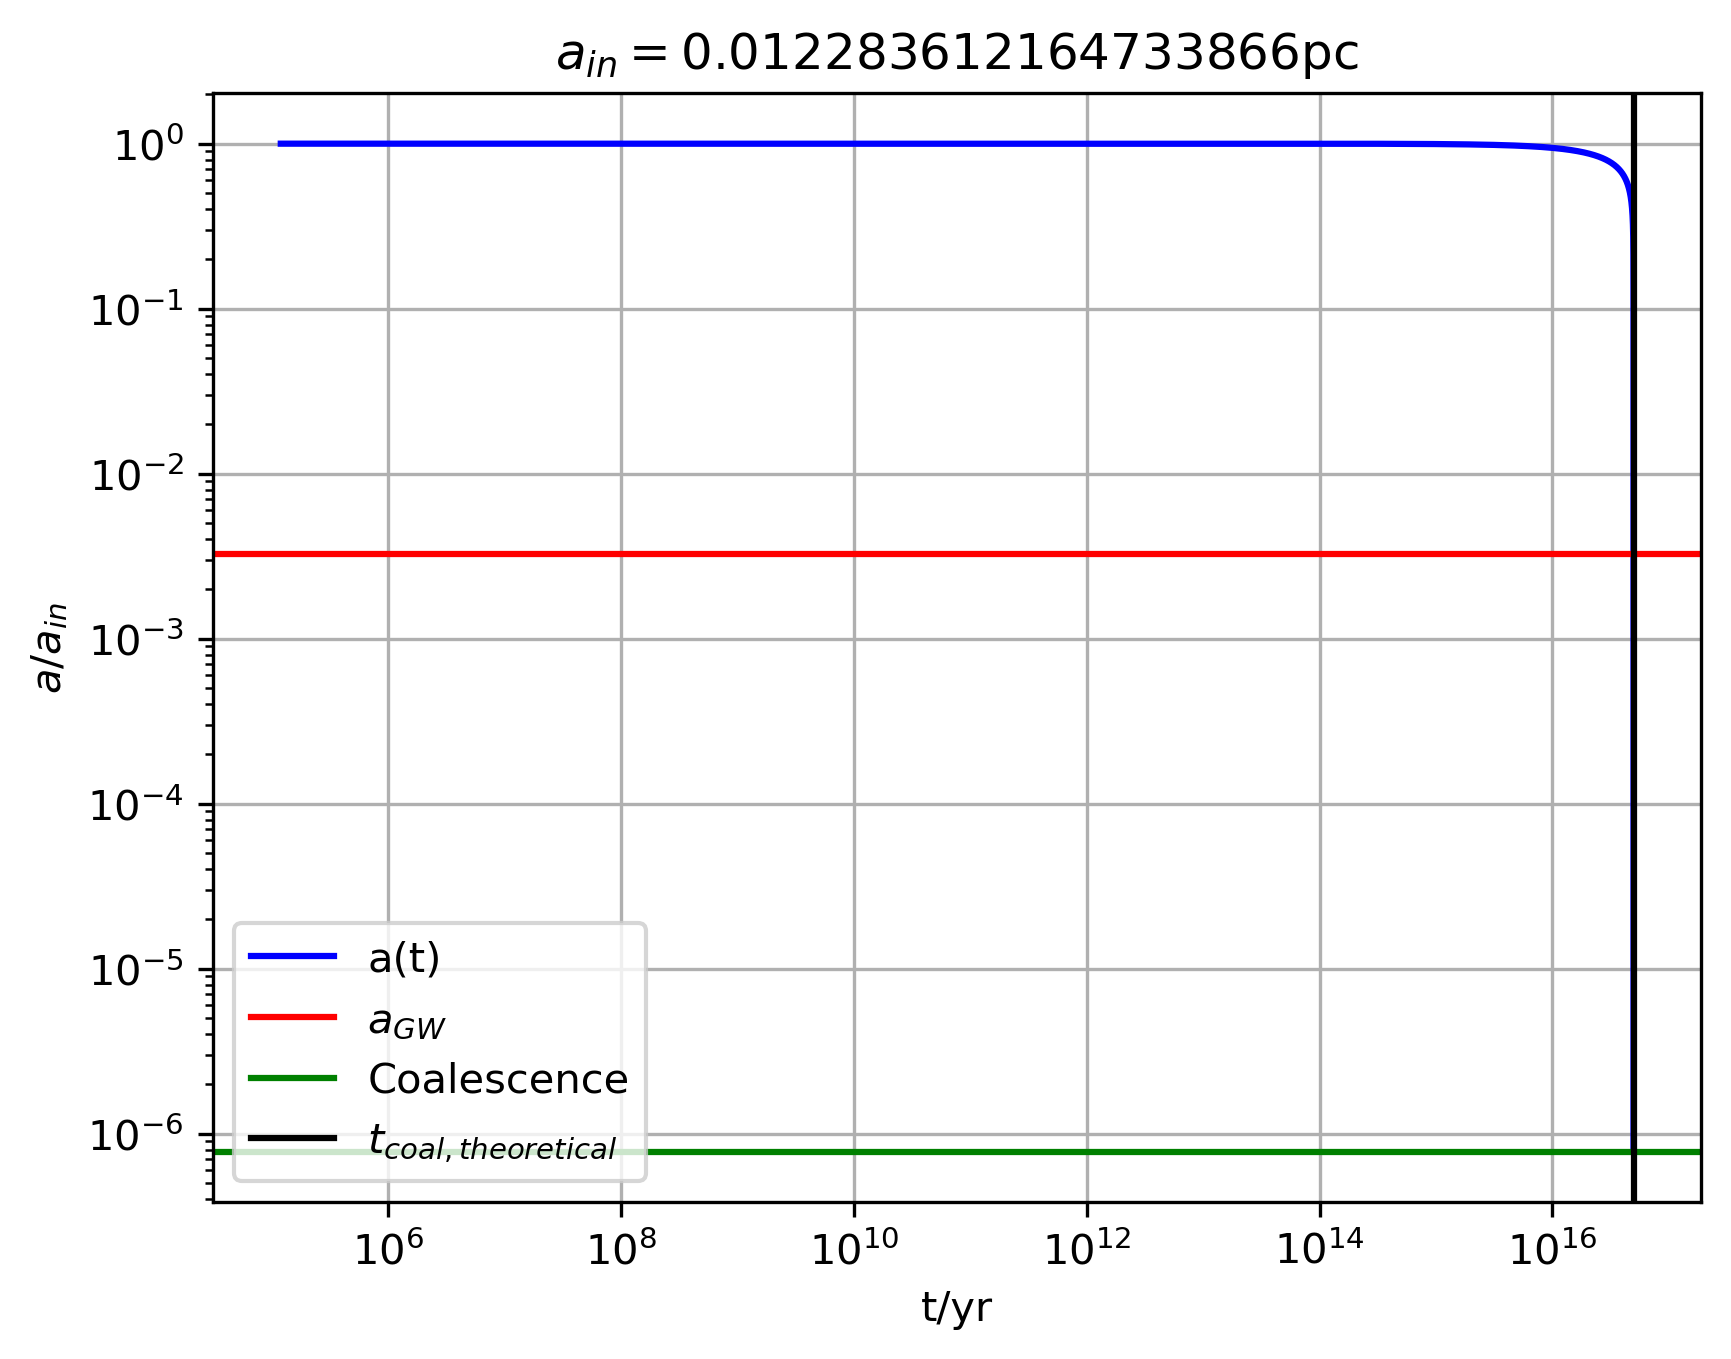
\includegraphics[height=5cm]{a_vs_t_GW.png}
    \caption{}
    \label{a_vs_t_GW}
    \vspace{2mm}
  \end{minipage}
  \hfill
  \begin{minipage}[c]{0.45\textwidth}
    \centering
    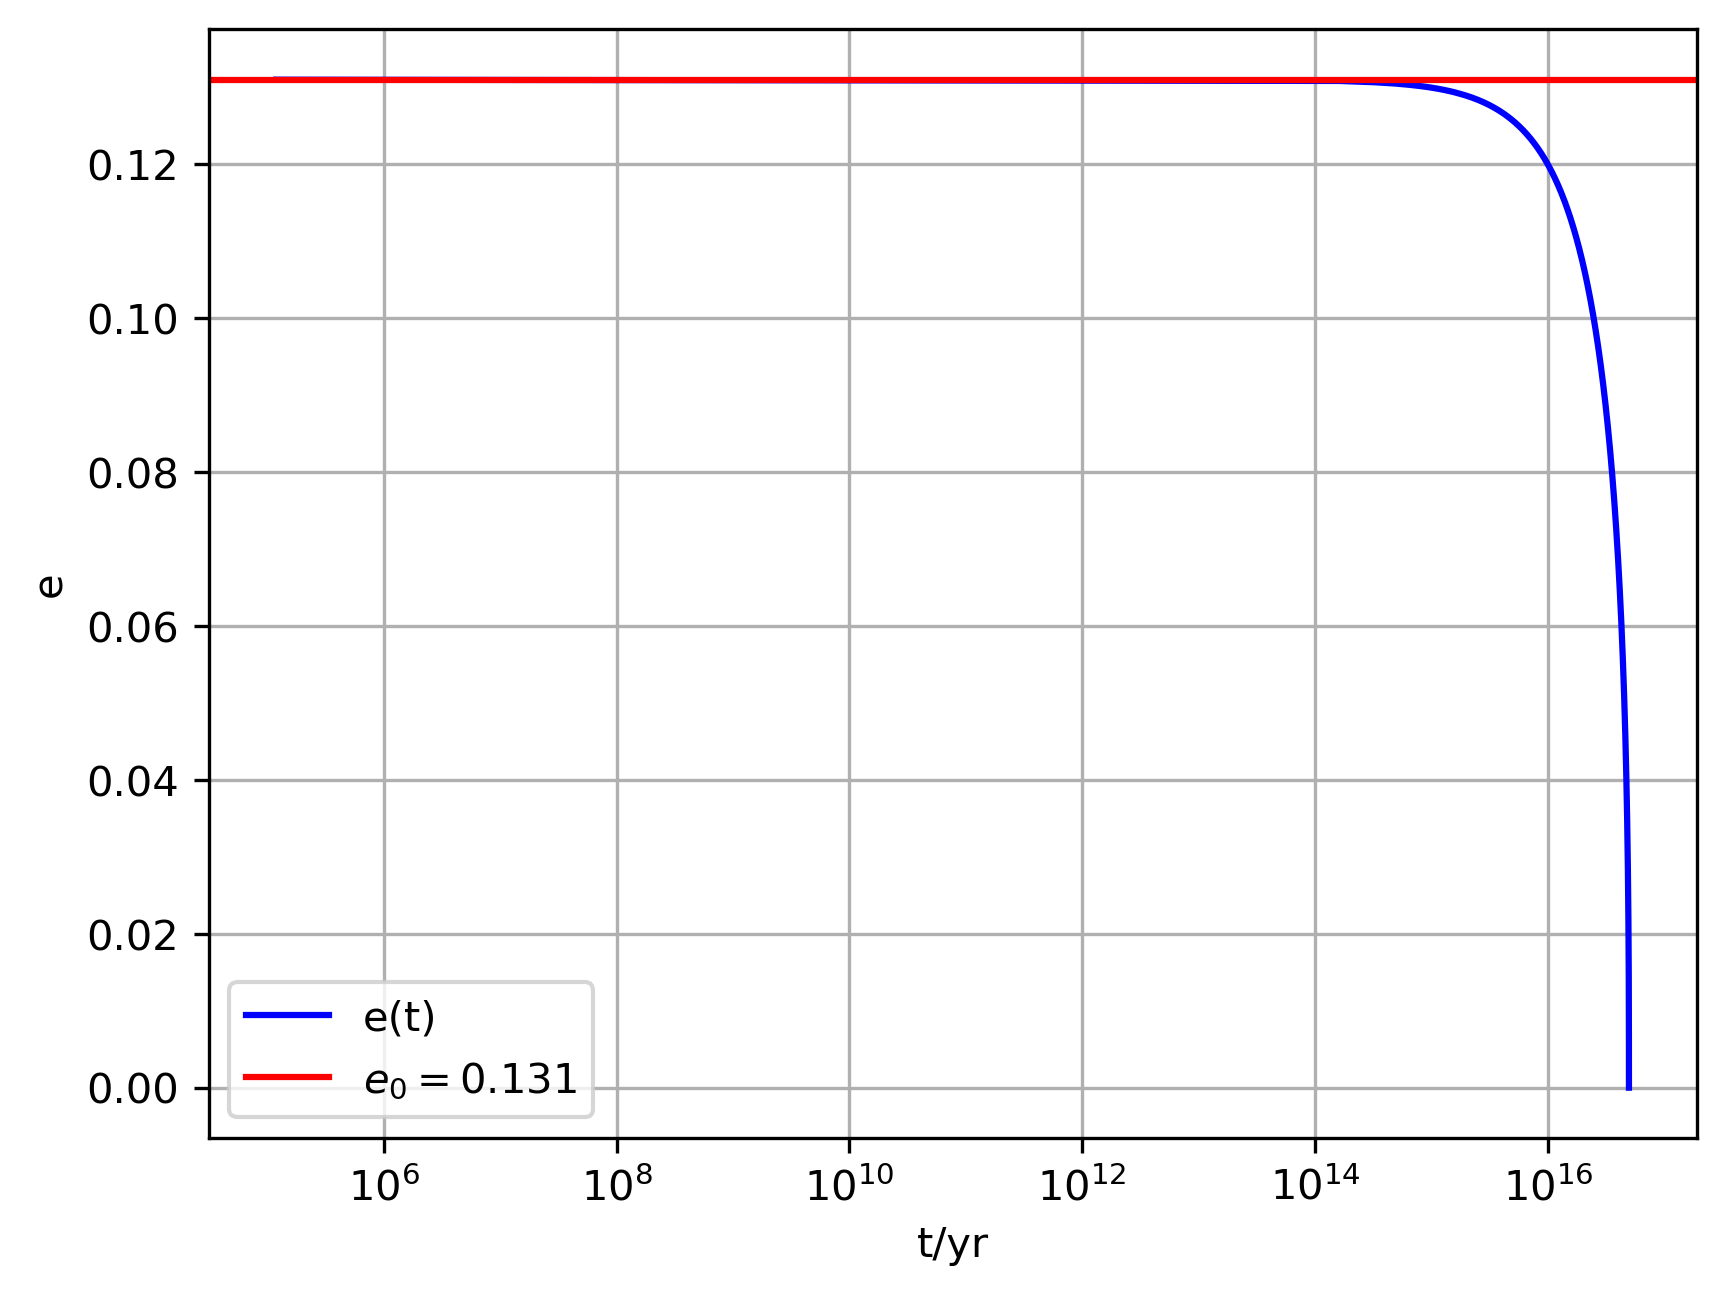
\includegraphics[height=5cm]{e_vs_t_GW.png}
    \caption{}
    \label{e_vs_t_GW}
    \vspace{2mm}
  \end{minipage}
\end{figure}



The dataset used above help us to construct another curve, precisely $(e(t,a(t)))$ which can be compared to the close form solution provided by Equation (\ref{a=a(e) Maggiore}) as shown in Figure \ref{a_vs_e_GW} and \ref{a_vs_e_Maggiore}.




\begin{figure}[H]
    \centering
  \begin{minipage}[c]{0.45\textwidth}
    \centering
    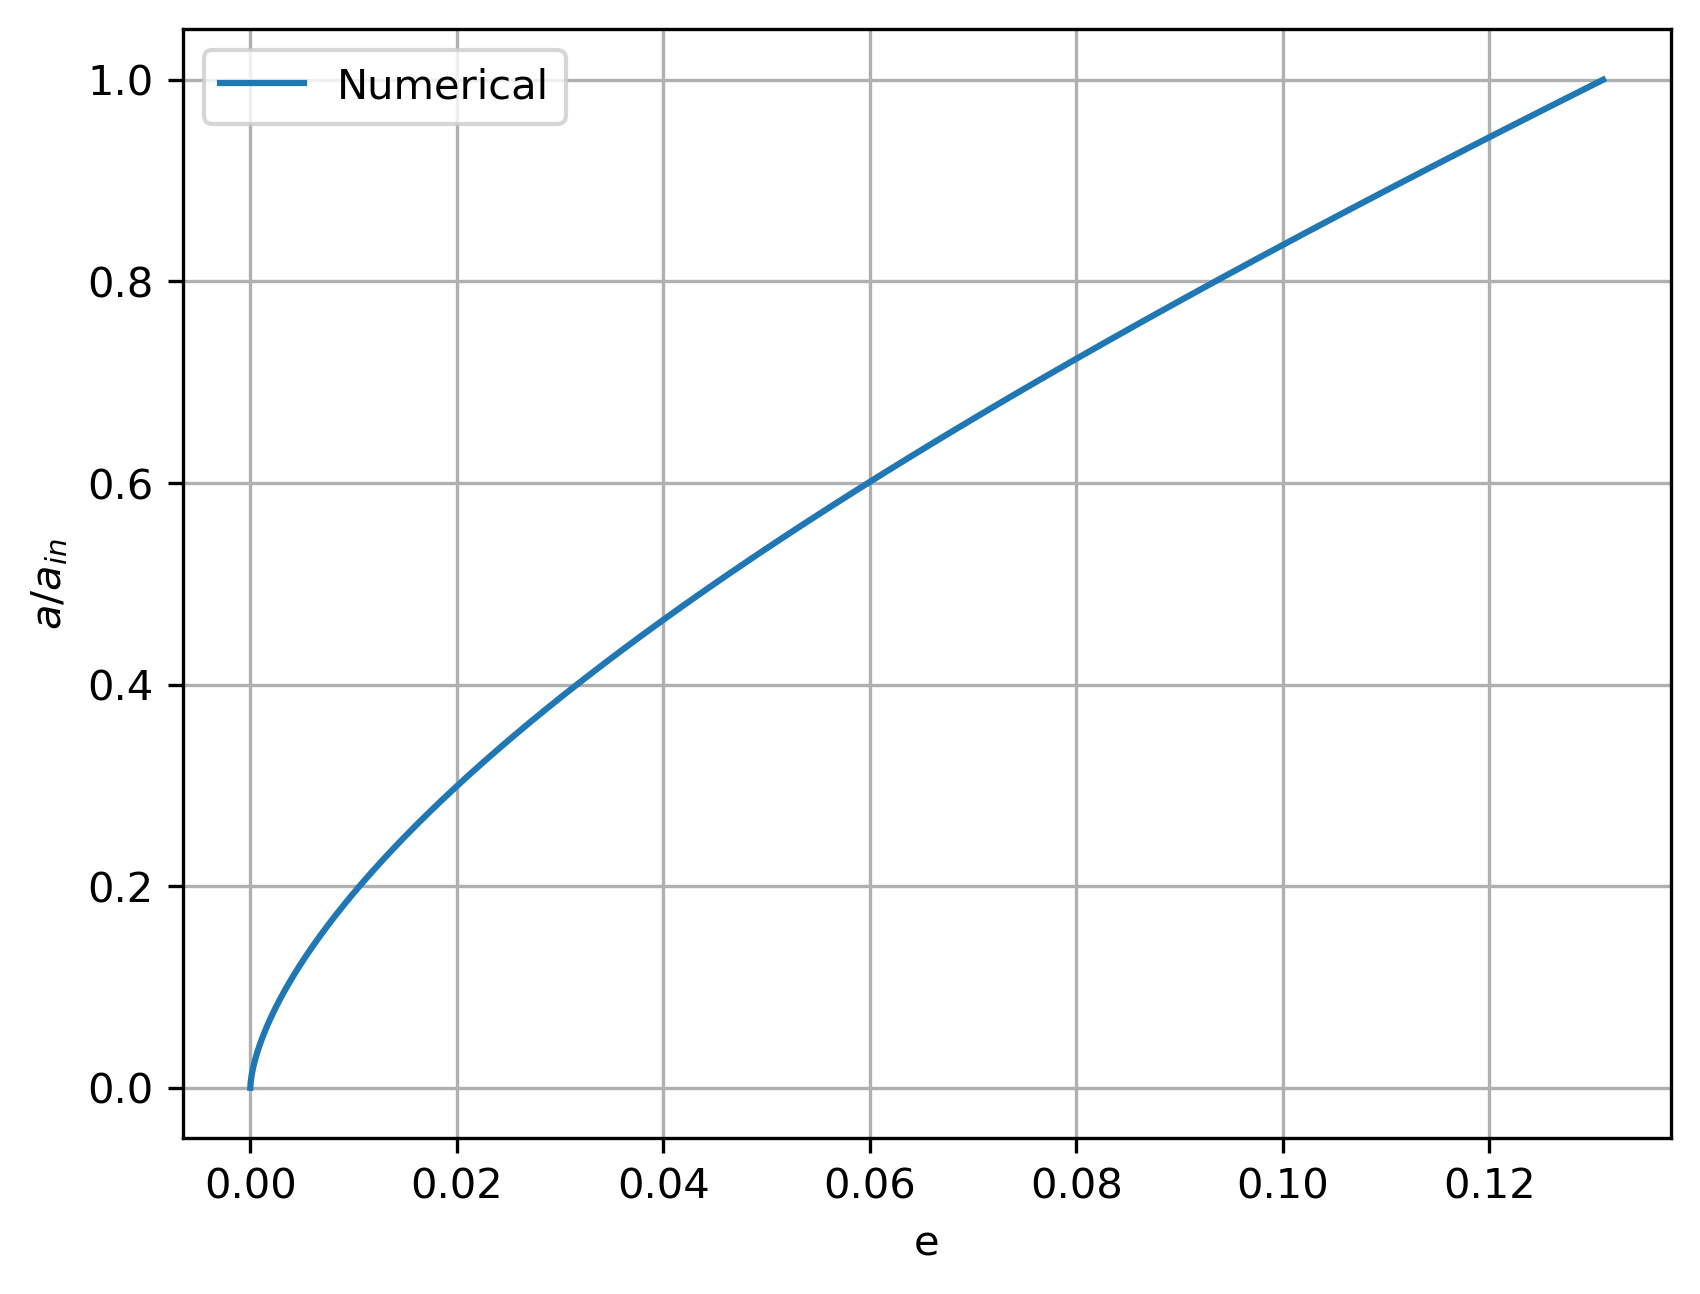
\includegraphics[height=5cm]{a_vs_e_GW.png}
    \caption{}
    \label{a_vs_e_GW}
    \vspace{2mm}
  \end{minipage}
  \hfill
  \begin{minipage}[c]{0.45\textwidth}
    \centering
    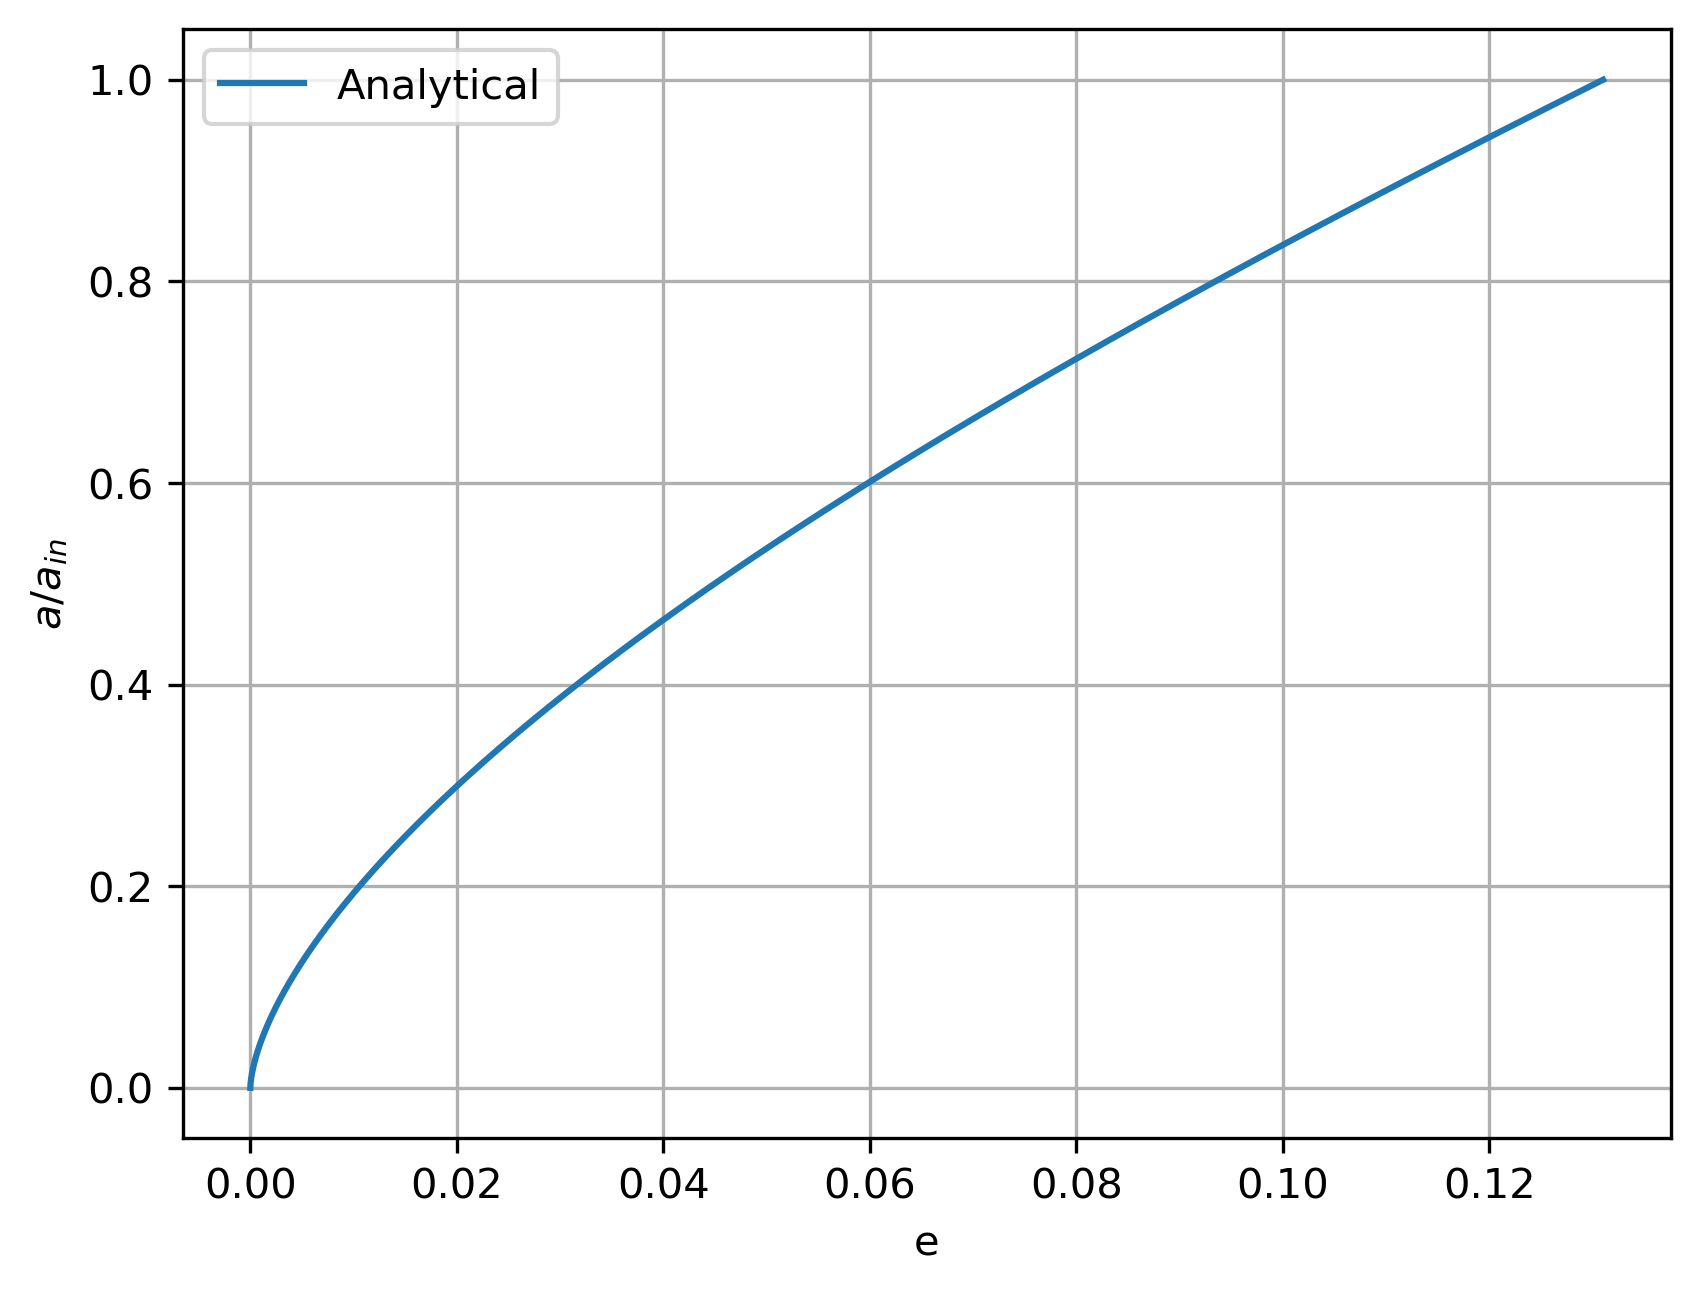
\includegraphics[height=5cm]{a_vs_e_Maggiore.png}
    \caption{}
    \label{a_vs_e_Maggiore}
    \vspace{2mm}
  \end{minipage}
\end{figure}


Below, the Figure \ref{error_a_vs_e_GW} gives us the possibility of visualizing the relative error of the numerical solution with respect to the analytical one; it turnsout to be within one part over $10^{12}$.


\begin{figure}[H]
    \centering
    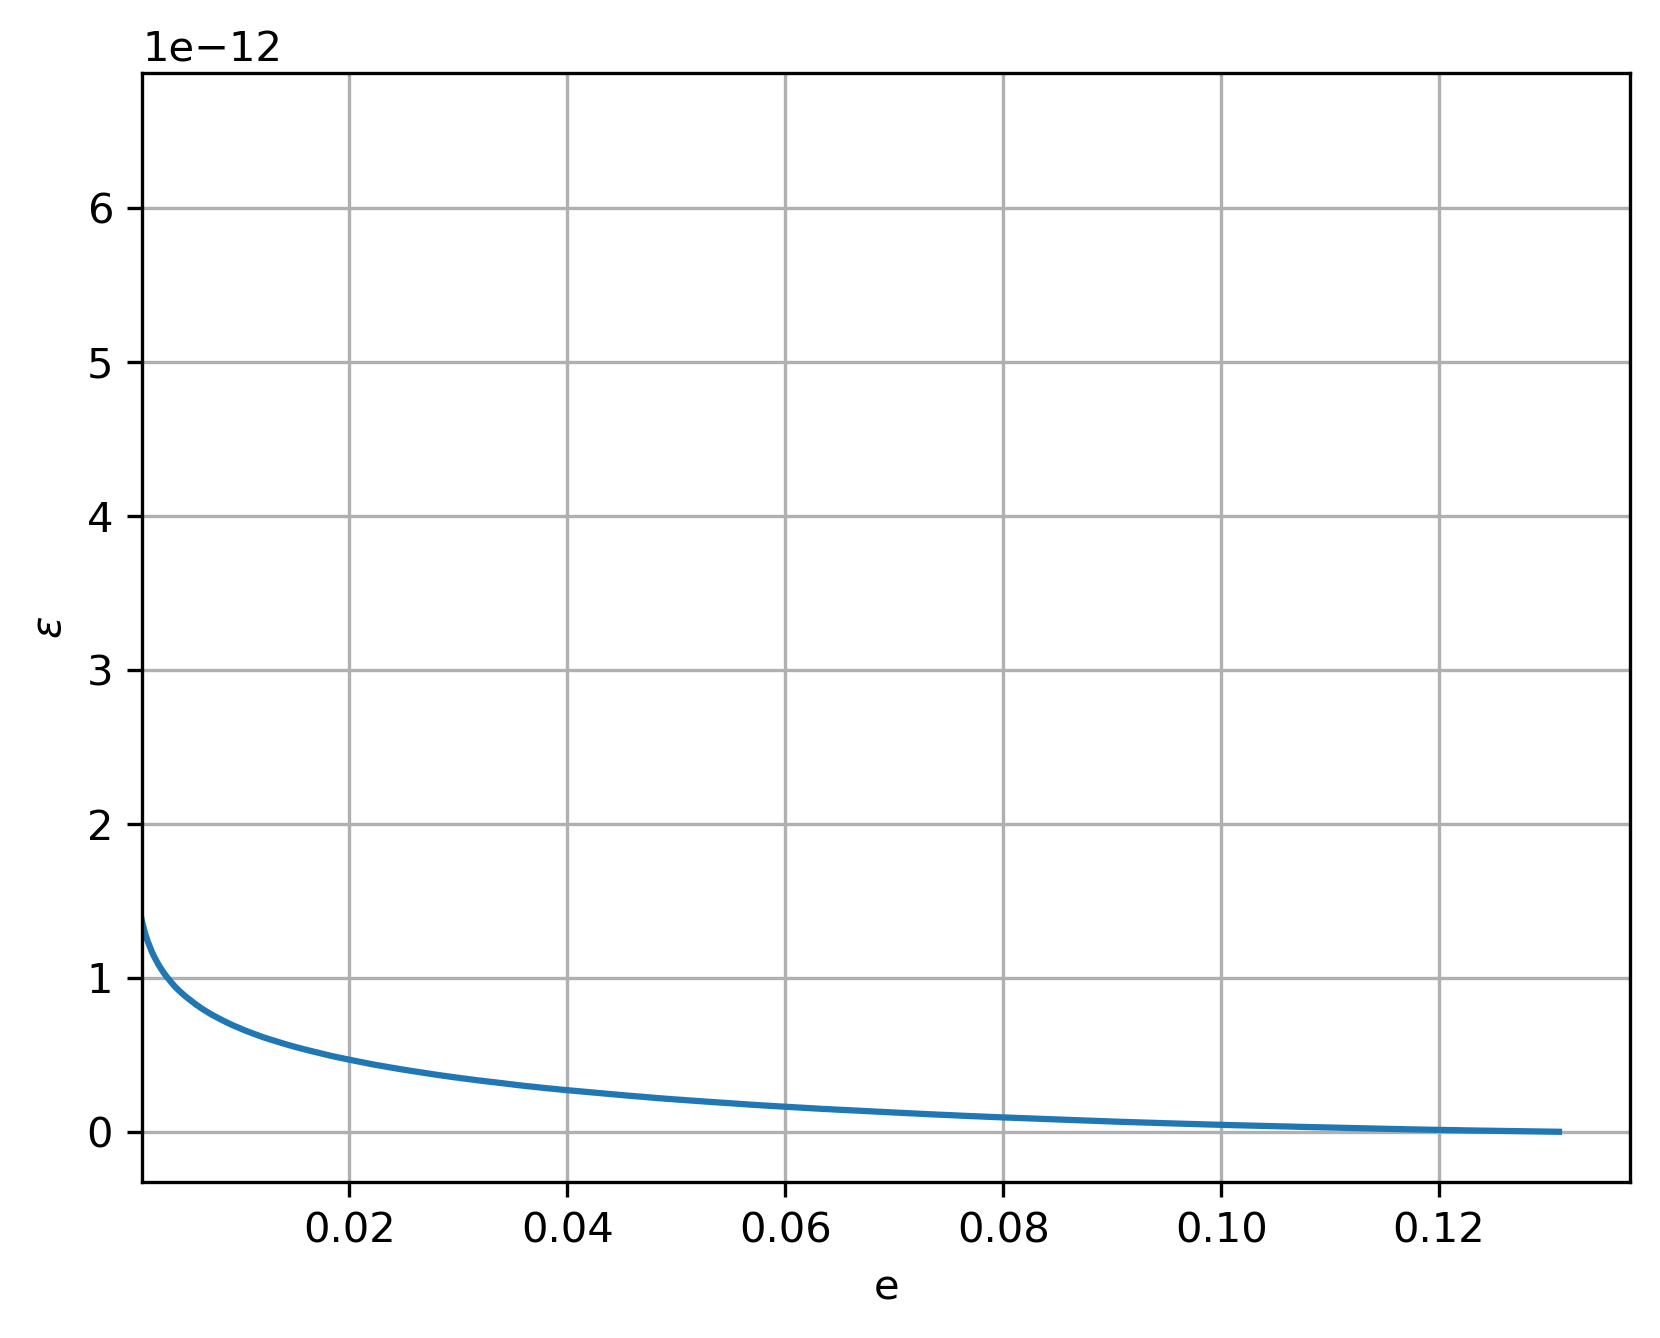
\includegraphics[width=0.5\linewidth]{error_a_vs_e_GW.png}
    \caption{}
    \label{error_a_vs_e_GW}
\end{figure}






\section{NGC 205 IMBH Binary evolution}

\subsection{NGC 205 Hybrid Model Evolution}
NGC 205 is a nearby dwarf galaxy with a NSC residing at its innermost region; it is belived to host an IMBH binary, whose estimated mass is $\sim 10^4 M_\odot$.\\The 2-D surface brightness profile of the dwarf, both the bulge and NSC treated as indipendent stellar components, is translated into 3-D Sersic density profile using Prugniel \& Simien \cite{Prugniel}:

\begin{equation}
    \rho(r)=\rho_0\left(\frac{r}{R_e}\right)^{-p}e^{-b\left(\frac{r}{R_e}\right)^{1/n}}.
\end{equation}
Here, $\rho_0$ is the density normalization unambiguously set by total galaxy mass, effective radius and Sersic index $n$; from \cite{Terzic}:
\begin{equation}
\rho_0
=
\frac{M_*}{4\pi R_e^3}
\frac{b^{\,n(3-p)}}{n\,\Gamma\!\left[n(3-p)\right]}.
\end{equation}
The parameters $p$ and $b$ can be expressed as a function of $n$ as follows: $p=1.0-0.6097/n+0.05563/n^2$, and $b \approx 2 n - 1/3 + 0.009876/n$, for $0.5 < n < 10$.\\Observations constrain the quantites $(M,R_{eff},n)$ for both bulge and NSC as reported in Figure (\ref{Khan_2021_NGC205}) of \cite{Khan_2021}.
\begin{figure}[H]
    \centering
    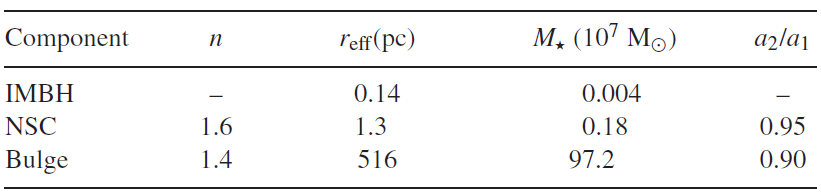
\includegraphics[width=0.5\linewidth]{Khan_2021_table.png}
    \caption{Column 1: Galaxy component. Column 2: Sersic index. Column 3:
Effective radius of the galaxy component (note: for the IMBH, we quote the
influence radius instead). Column 4: Stellar mass. Column 5: 2D axial ratio
as measured by GALFIT.}
    \label{Khan_2021_NGC205}
\end{figure}

Numerically it is found
\begin{itemize}
    \item Bulge: $\rho_0=4.80\cdot 10^5M_\odot/pc^3$
    \item NSC: $\rho_0=2.95M_\odot/pc^3$
\end{itemize}
and NGC 205 density profile is reconstructed in  Figure (\ref{NGC205 density profile}).

\begin{figure}[H]
    \centering
    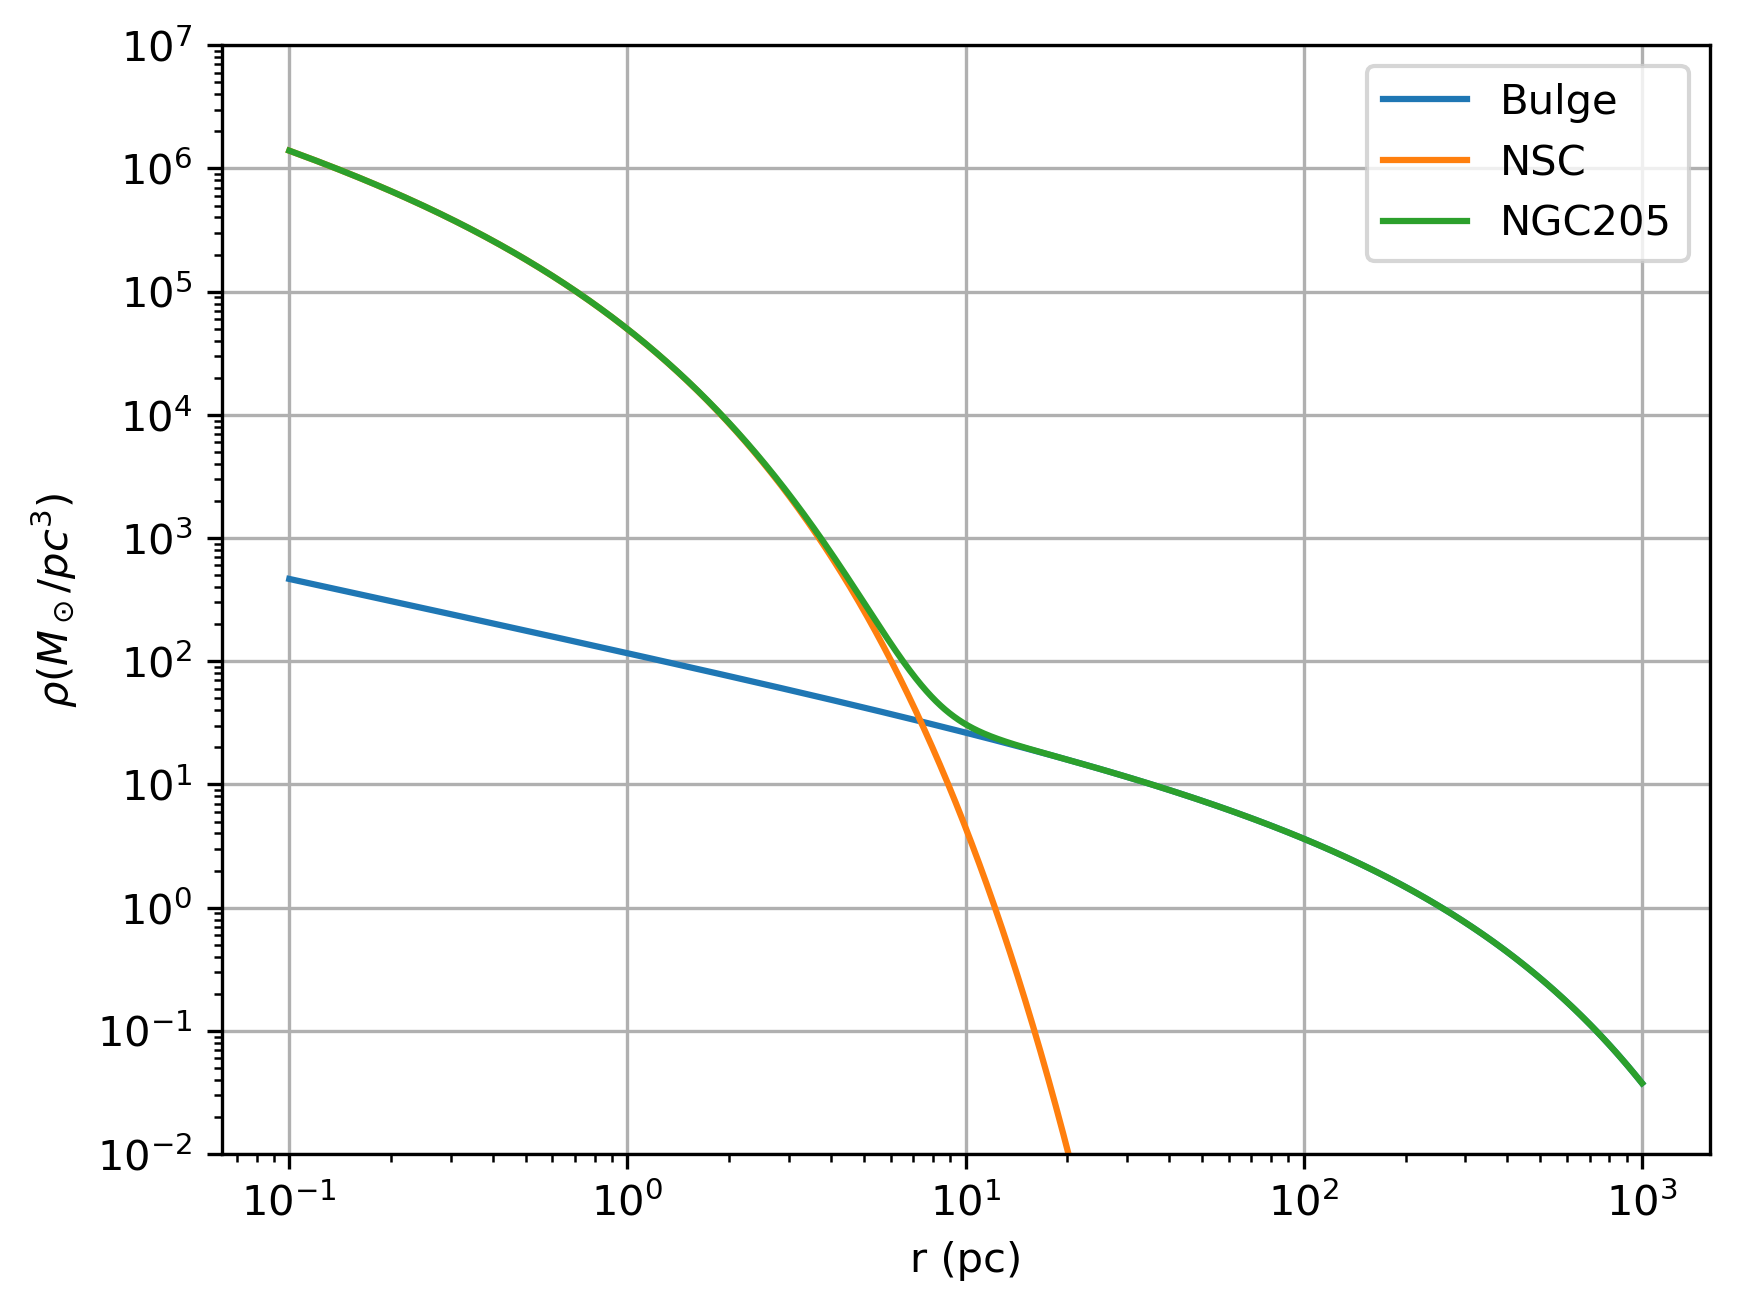
\includegraphics[width=0.5\linewidth]{NGC205_density_profile.png}
    \caption{NGC 205 bulge, NSC and total mass density profile of stellar distribution.}
    \label{NGC205 density profile}
\end{figure}
Adopting the same prescription of \cite{Khan_2021} and \cite{Holley-Bockelmann_2025}, a symmetric IMBH binary of masses $M_1=M_2=4\cdot10^4M_\odot$ is introduced into NGC 205 core and its evolution, due to stellar and GWs hardening, is tracked combining 3-body scattering experiment hybrid model \cite{Quinlan_1996},\cite{Sesana_2006} and \cite{Peters_1963} equations.\\It is quite relevant to point out that in this astrophysical system the hardening due to bound stars \cite{Sesana_2008} is negligible in light of the symmetry of the binary and the arguments exposed at the end of Sec.(\ref{sec:Loss Cone}).\\Therefore, combining the set of equations related to Unbound evolution
\begin{equation}\label{da/dt UNBOUND}
    \frac{da}{dt}|_u = -\frac{a^2 G \rho_{\mathrm{inf}}}{\sigma}  H
\end{equation}

\begin{equation}\label{de/dt UNBOUND}
    \frac{de}{dt}|_u = \frac{a G \rho_{\mathrm{inf}}}{\sigma}  H K
\end{equation}
and the equations describing GWs driven hardening \ref{da/dt Peterson} \ref{de/dt Peterson}, the set of differential equations must be solved reads

\begin{equation}\label{da/dt Un+GW}
    \frac{da}{dt} = \frac{da}{dt}|_u+\frac{da}{dt}|_{gw}
\end{equation}

\begin{equation}\label{de/dt Un+GW}
    \frac{de}{dt} = \frac{de}{dt}|_u+\frac{de}{dt}|_{gw}
\end{equation}
Although the original formulation of the hybrid model relies on a SIS profile, with very peculiar features (i.e. costant velocity dispersion), Sesana \cite{Sesana_2015} showed how to use it for a more general stellar background. The vast majority of stars, unbound to the binary, refilling the loss cone (i.e. having pericenter $\sim a$) come from a region that is just beyond the binary influence radius, hence $r_{inf}$ is the relevant physical scale of the model and $\sigma$ appearing in Equations \ref{da/dt UNBOUND} and \ref{de/dt UNBOUND}, which is in general a function of the radius for spherically symmetric systems, must be computed at the influence radius (here defined as the radius enclosing stellar mass that is twice the binary one).\\Apart from setting the inital point in the $(a,e)$ space, we need to determine several quantities; we start with binary influence radius and $\sigma_{inf}=\sigma(r_{inf})$; they both require the knowledge of the cumulative mass $M(<r)$ associated to the Sersic profile. It results from the integration of $\rho(r)$ and admits analytic solution \cite{Terzic}
\begin{equation}
M(<R)
=
M_{\rm tot}\,
\frac{
\gamma\!\left(
2n,\;
b_n \left(\frac{R}{R_e}\right)^{1/n}
\right)
}{
\Gamma(2n)
}.
\end{equation}
The root of the equation
\begin{equation}
    M(<r_{inf})-2(M_1+M_2)=0
\end{equation}
is obtained numerically by bisection and holds $r_{inf}=0.47pc$.\\On the other hand, Jeans equation provides a way to compute the velocity dispersion and in case of spherical distributions it greatly simpifies to
\begin{equation}\label{Jeans velocity dispersion equation}
\sigma^2(r) =
\frac{1}{\rho(r)}
\int_r^\infty
\rho(s)\,\frac{G M(<s)}{s^2}
ds.
\end{equation}
The integral leads to $\sigma_{inf}=$32.6km/s.
As both $\sigma(r)$ and the circular speed $V_c(r)=\sqrt{GM(<r)/r}$ depend on $M(<r)$, previously obtained, we can derive them and Figure \ref{sigma/Vc NGC205} displays their ratio as afunction of the radius.  


\begin{figure}[H]
    \centering
    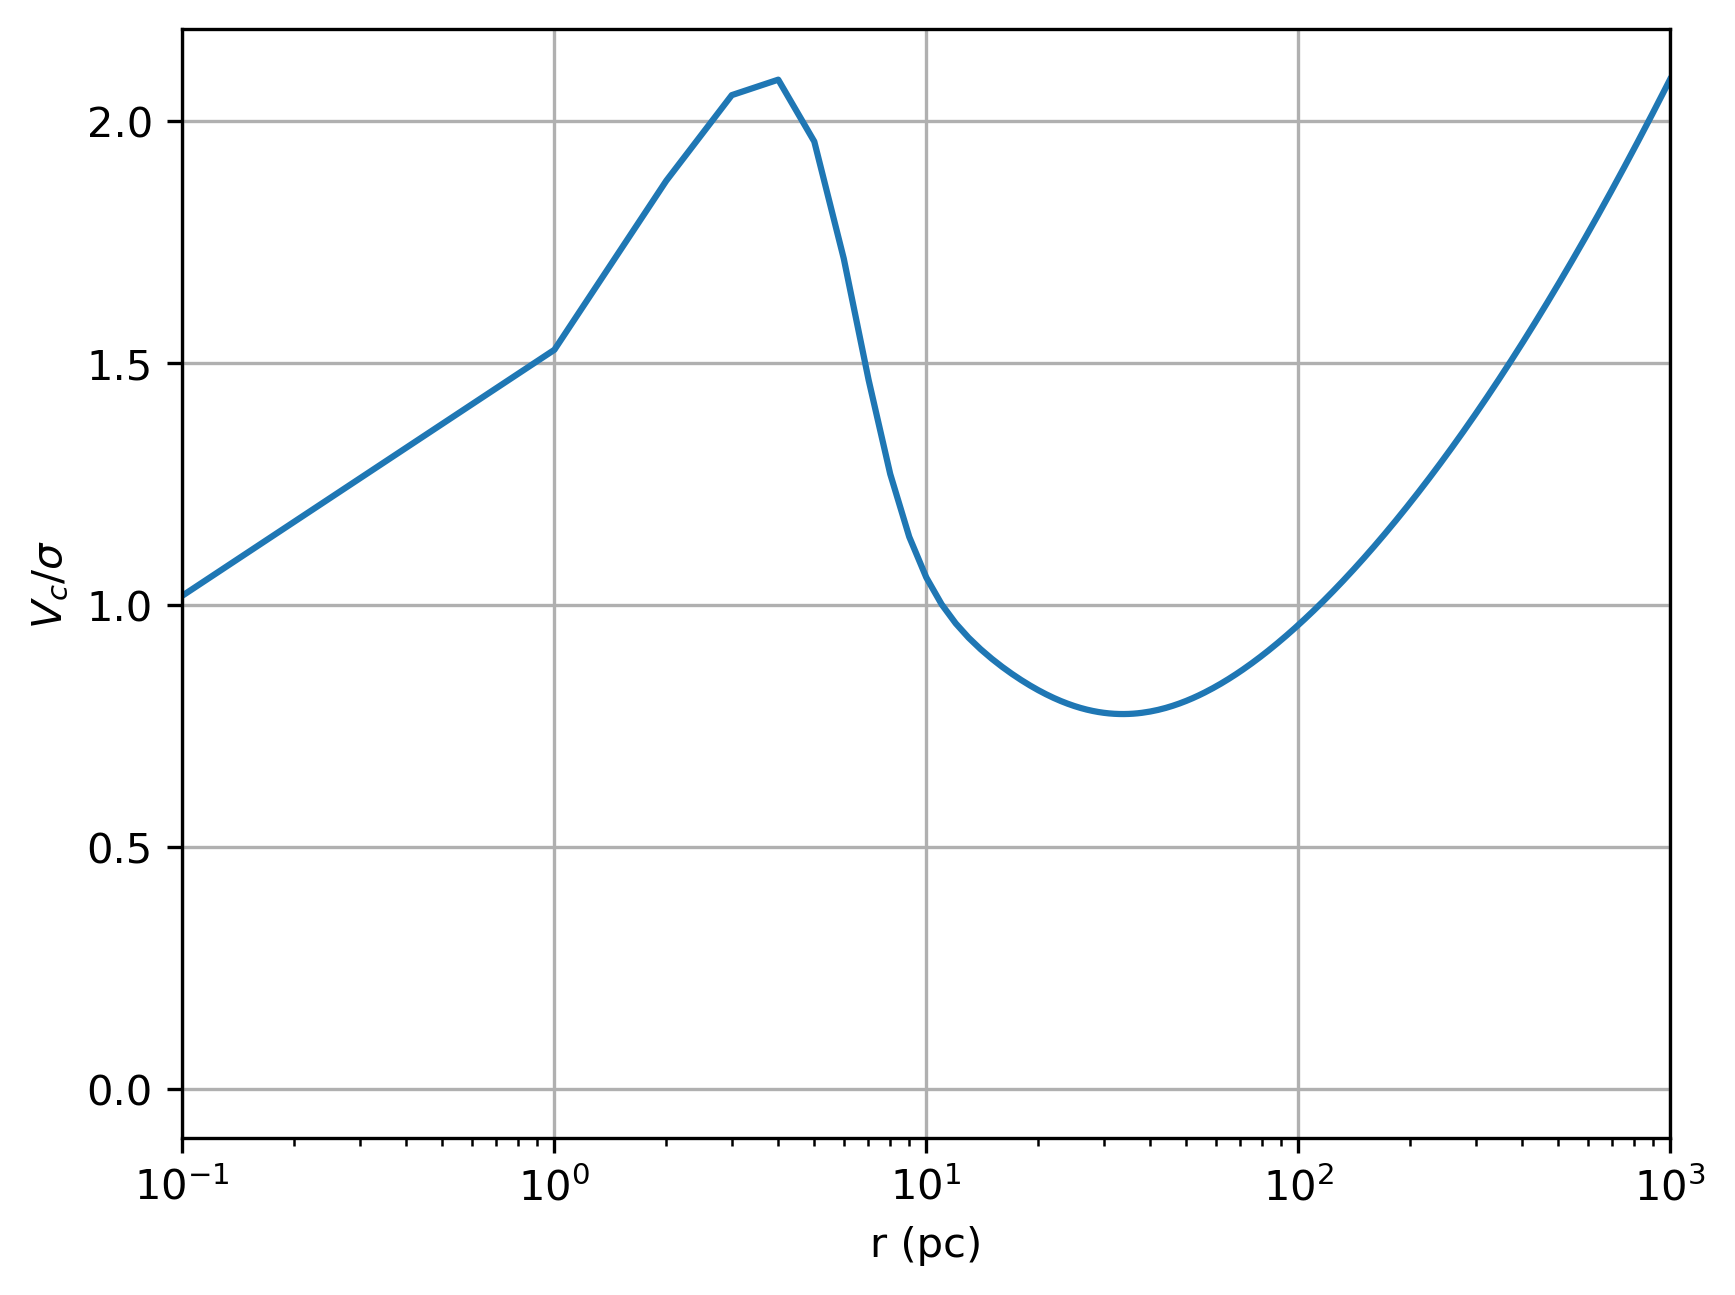
\includegraphics[width=0.5\linewidth]{NGC205_Vc_over_sigma_profile.png}
    \caption{NGC 205 $V_c/\sigma$ vs r}
    \label{sigma/Vc NGC205}
\end{figure}

The last quantity we have to specify in order to implement the hybrid model is the binary hardening radius $a_h$; indeed Sesana \cite{Sesana_2006} found out from 3-body scattering experiments that $H$ and $K$ functions can be fitted to
 \begin{equation}
     H=A(1+a/a_0)^\gamma
\end{equation}
and
 \begin{equation}
    K=A(1+a/a_0)^\gamma+B
\end{equation}
The parameters of the fits to H and J are listed in Tables 1 and 2 of \cite{Sesana_2006} for different binary mass ratios and eccentricity; there, $a_0$ is given in $a_h$ units, thus forcing us to determine it. In literature several definitions have been proposed; hereafter, we will be using
\begin{equation}\label{a_h dynamical definition}
    a_h\approx \frac{GM_2}{4\sigma^2},
\end{equation}
unless otherwise stated. This definition leads to $a_h\approx 0.04 pc$.\\We can finally proceed and numerically integrate the set of equations \ref{da/dt Un+GW} and \ref{de/dt Un+GW} by means of R-K(4). For the temporal evolution to be properly resolved from the initial configuration to the coalescence of the binary, the time step adjusts itself at each iteration, thus taking care of whether the dominant timescale is set by stellar hardening or GWs hardening at that time.\\By defining 
\begin{equation}
    \Delta t_i=\epsilon \cdot min\left(\frac{a}{|da/dt|_u},\frac{a}{|da/dt|_{gw}}\right),
\end{equation}
where $\epsilon\sim 10^{-3-4}$, and the initial conditions $(a_0,e_0)=(15pc, 0.7)$, the integration returns $a(t)$ and $e(t)$.\\They are shown in Figure \ref{NGC205 a vs t} and \ref{NGC205 e vs t}.

\begin{figure}[H]
    \centering
    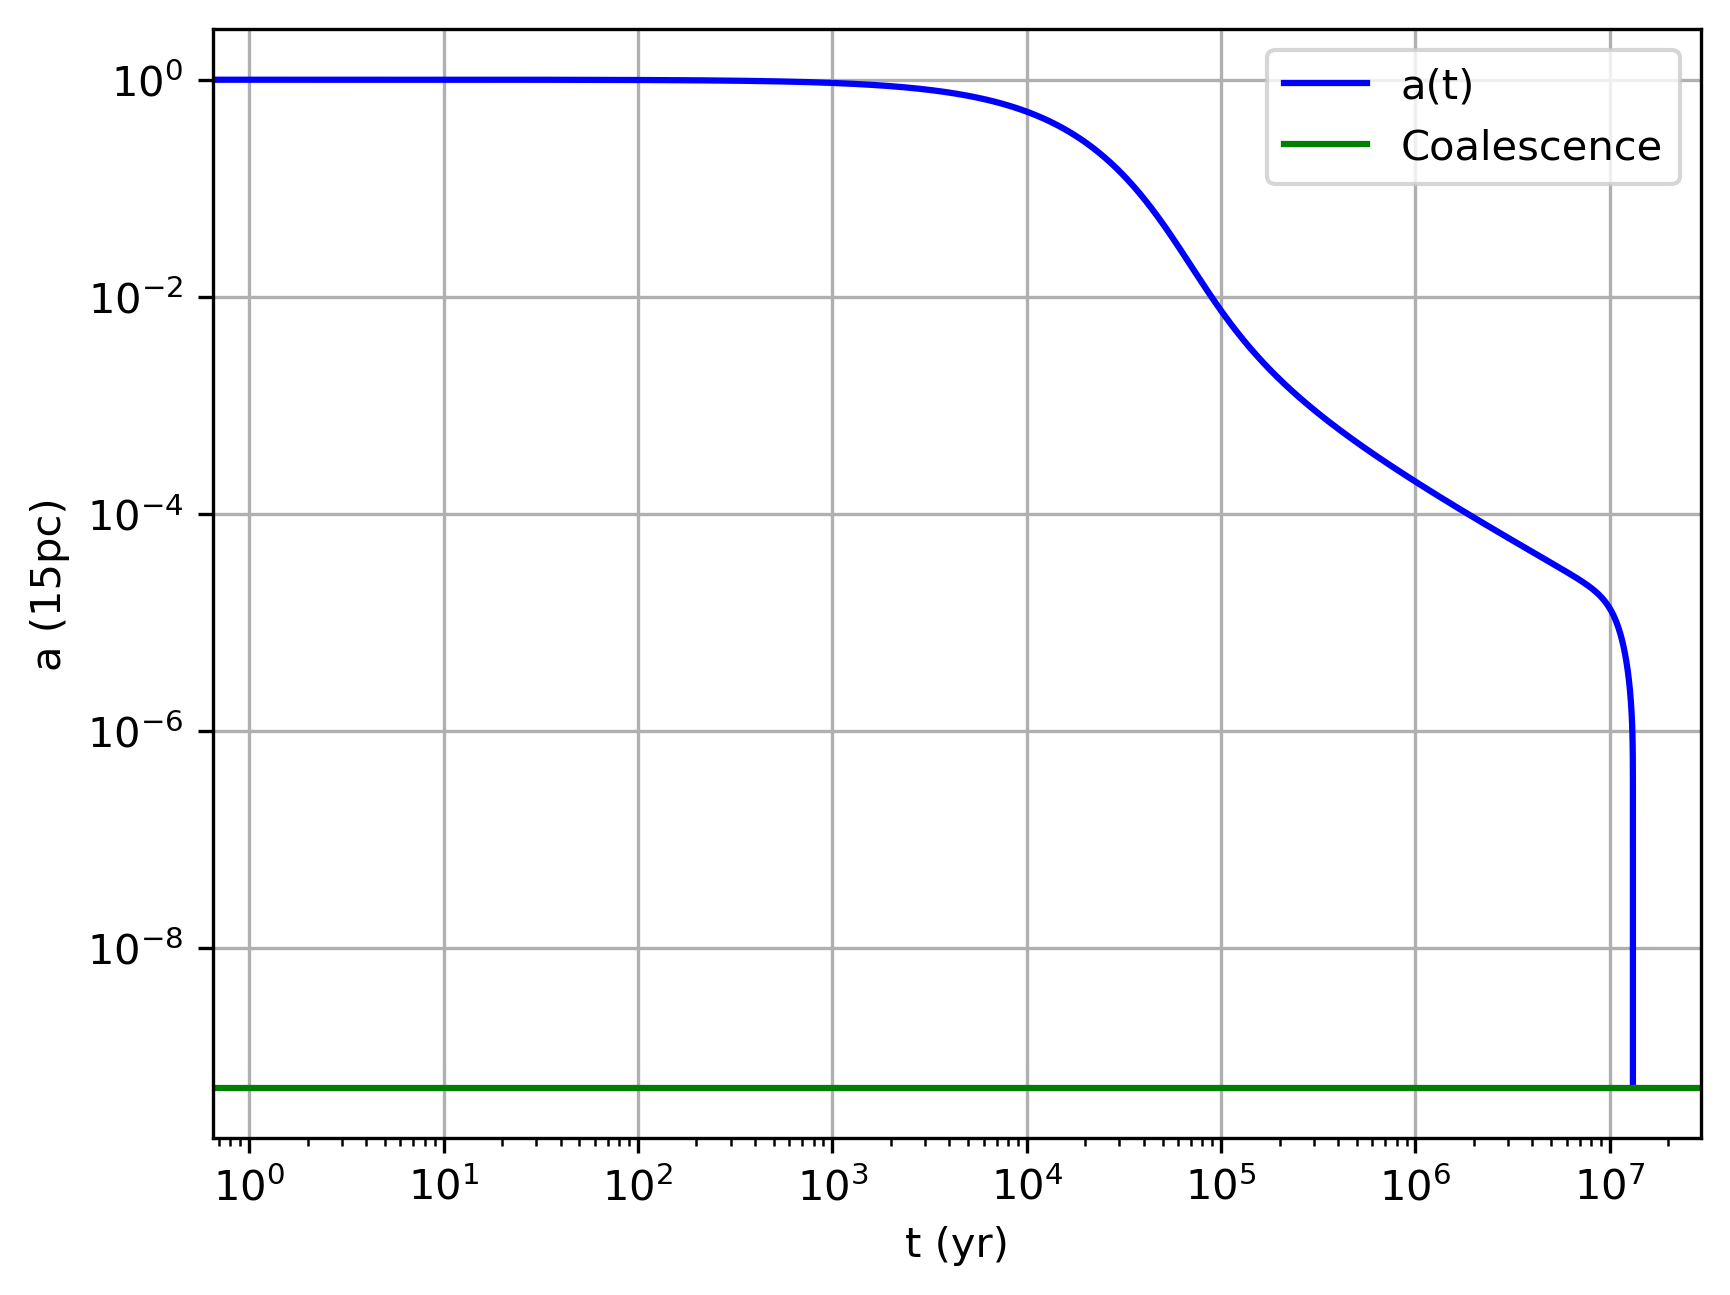
\includegraphics[width=0.5\linewidth]{NGC205_a_vs_t.png}
    \caption{NGC 205 a vs t}
    \label{NGC205 a vs t}
\end{figure}


\begin{figure}[H]
    \centering
    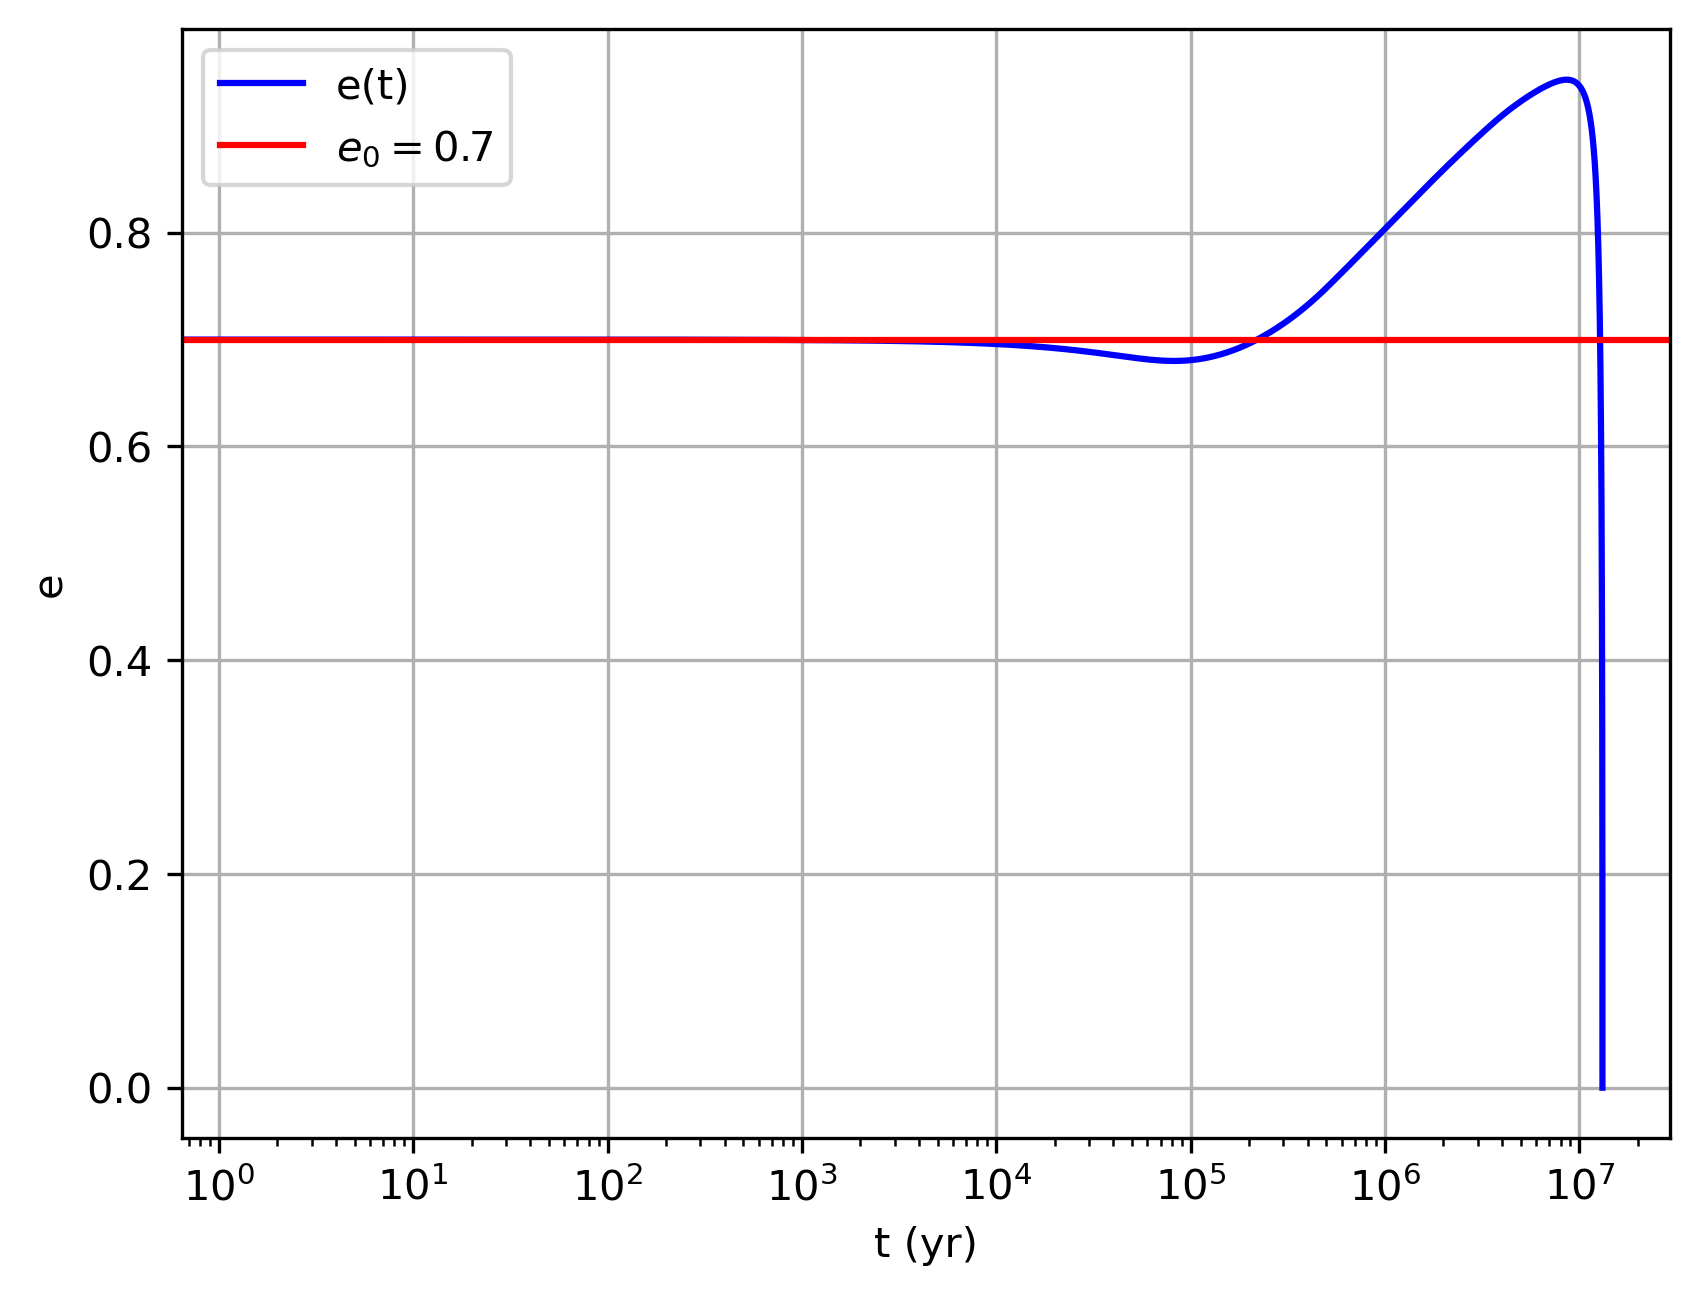
\includegraphics[width=0.5\linewidth]{NGC205_e_vs_t.png}
    \caption{NGC 205 e vs t}
    \label{NGC205 e vs t}
\end{figure}

The estimeted coalescence time is $t_{coal}=13.15 Myr$; it is of the same order of magnitude of\cite{Khan_2021} and \cite{Holley-Bockelmann_2025} predictions of $t_{coal}=74Myr$.\\$\mathbf{NOTE}$: Khan estimate comes from N-body simulations and in the special case of NGC 205 a costant value of eccentricity $e=0.39$ is assumed for the late evolution of the binary.\\Assuming a reliable time (universal time) at which the binary is in the configuration $(a_0,e_0)$ it might be interesting to get an estimate of the corresponding $z_{coal}$ from
\begin{equation}
t(z) = \int_z^{\infty}
\frac{dz'}{(1+z')H(z')}
\end{equation}
and compare it with LISA upper limit $(z\sim20)$, hence addressing the problem of a possible detection.\\If the binary is in the initial configuration at $z\approx 10$, it will coalesce at $z\approx 9.4$.

\subsection{Cosmic Size Evolution Down to NGC 205}
Here, we explore the importance of the existence of NSC to the binary evolution and coalescence time. A such structure is expected to drastically reduce the time taken by system to merge as a consequence of the larger number of stars capable of passing close to the binary.\\In this spirit, we will be referring to the same parameters table a procedure of the prevois SubSection but the NSC which is artificially removed from the dwarf galaxy; hence, the only stellar background affecting binary evolution is the stellar bulge.\\By repeating the same analysis and setting $(t_0,a_0,e_0)=(0yr,15pc,0.7)$, we show Figure \ref{NGC205 bulge a vs t plot} and \ref{NGC205 bulge e vs t plot}.

\begin{figure}[H]
    \centering
    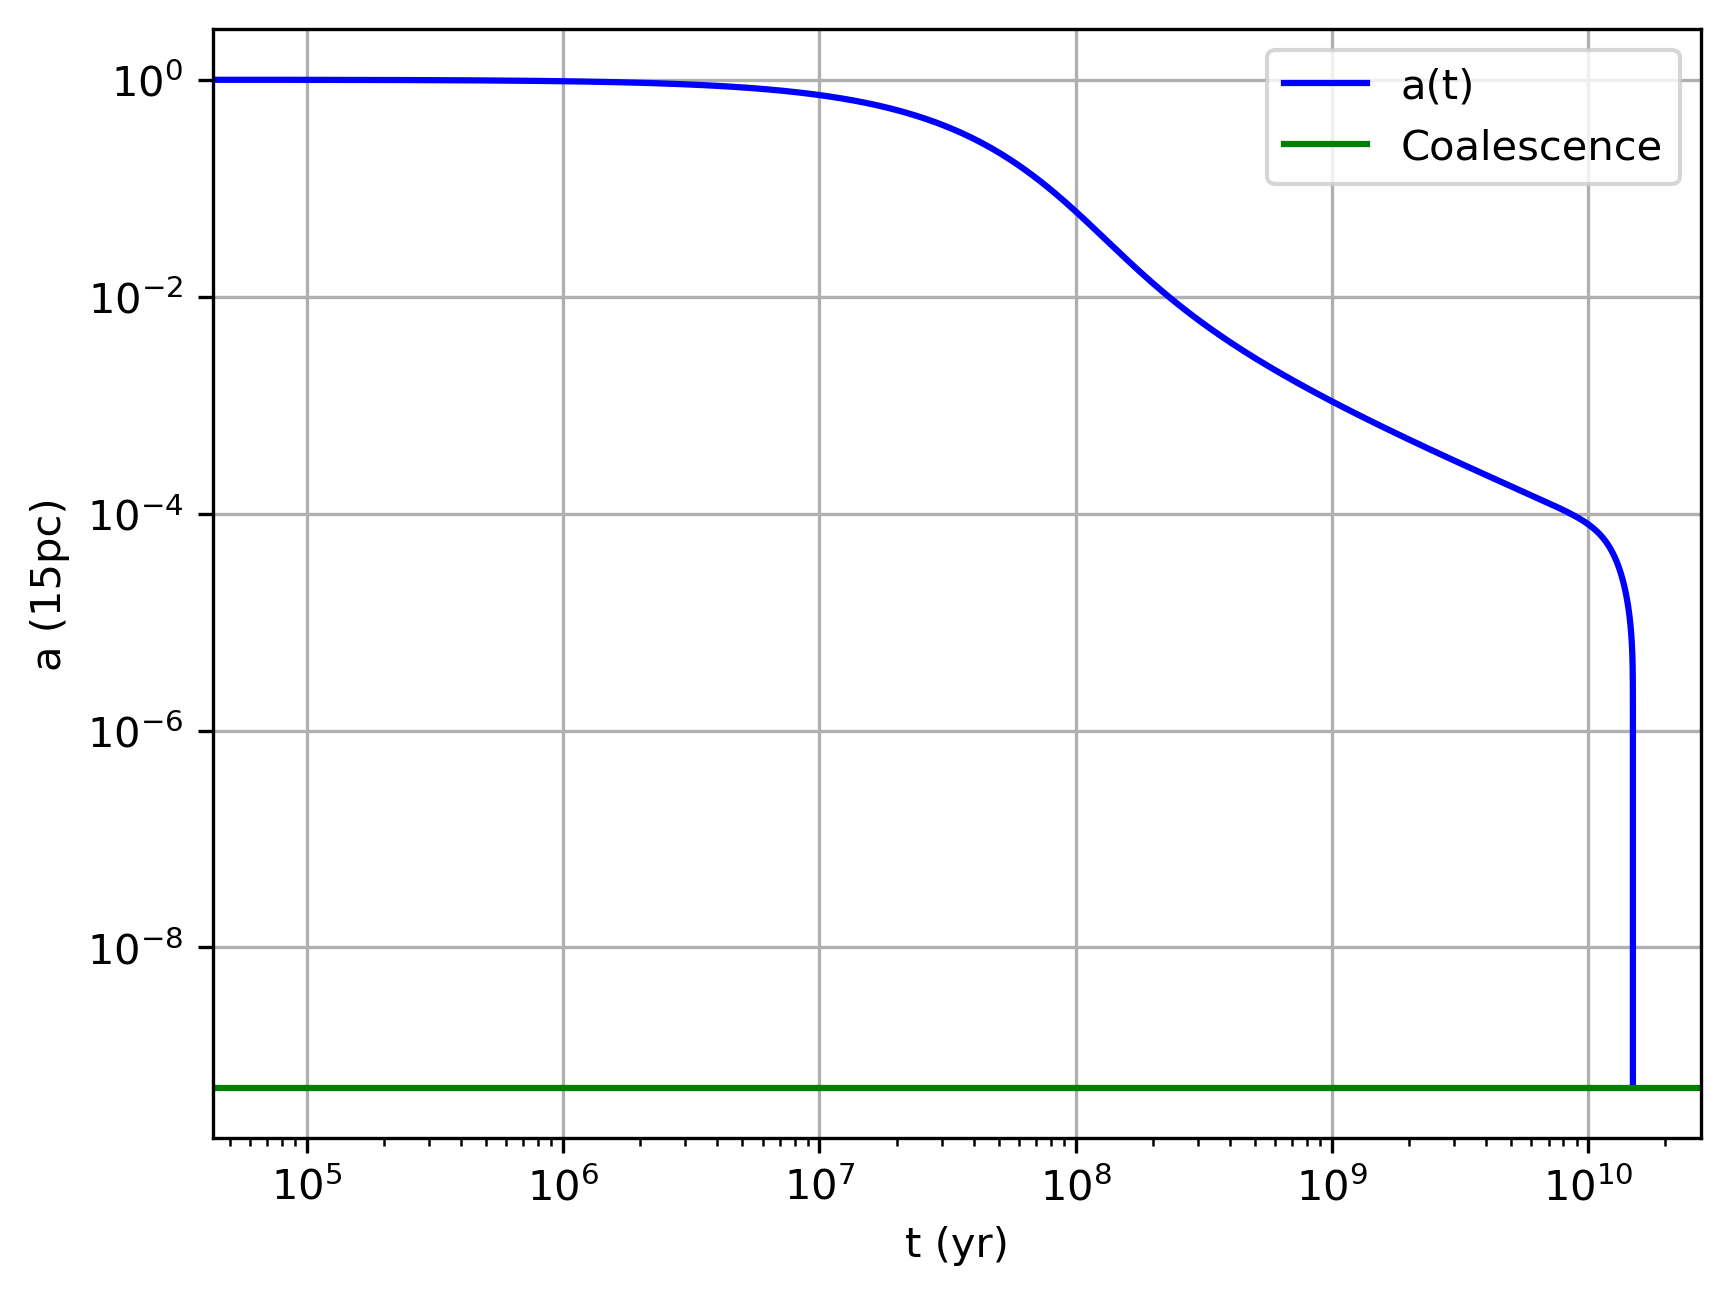
\includegraphics[width=0.5\linewidth]{NGC205_Bulge_a_vs_t.png}
    \caption{}
    \label{NGC205 bulge a vs t plot}
\end{figure}

\begin{figure}[H]
    \centering
    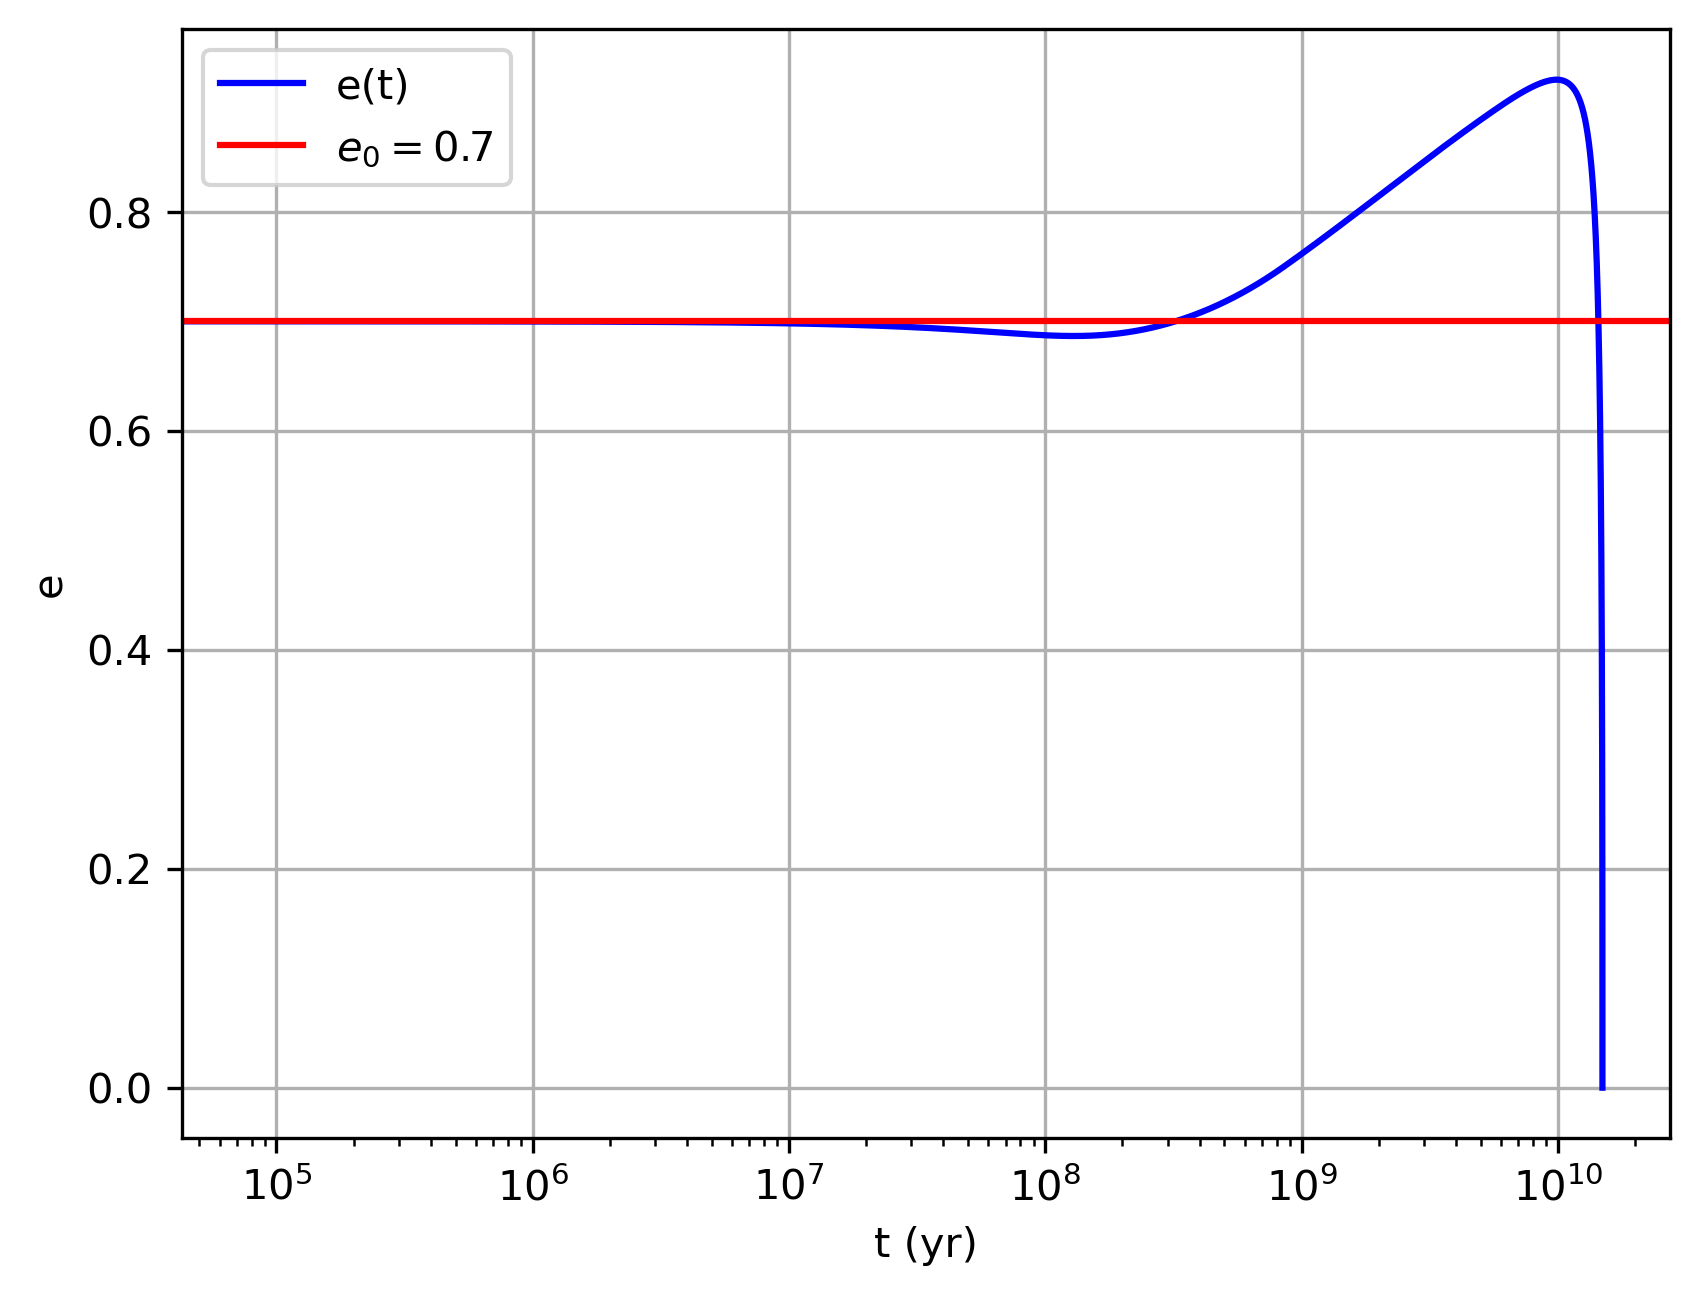
\includegraphics[width=0.5\linewidth]{NGC205_Bulge_e_vs_t.png}
    \caption{}
    \label{NGC205 bulge e vs t plot}
\end{figure}

Now $t_{coal}=14.93 Gyr$, almost three orders of magnitude longer than the NSC scenario.\\Following Ono cosmic size evolution relation $R_{eff}(z)=R_{eff}(z=0)(1+z)^{-1.22}$ \cite{Ono_2023}, we take NGC 205 as a $z=0$ reference model and we discuss the evolution of the same IMBH binary inside its plausible progenitors distributed between $z=1$ and $z=20$. All galaxies share same bulge mass and Sersic index; density profiles differ from each other only because of the different effective radius as diplayed in Figure \ref{Cosmic size density plot}.

\begin{figure}[H]
    \centering
    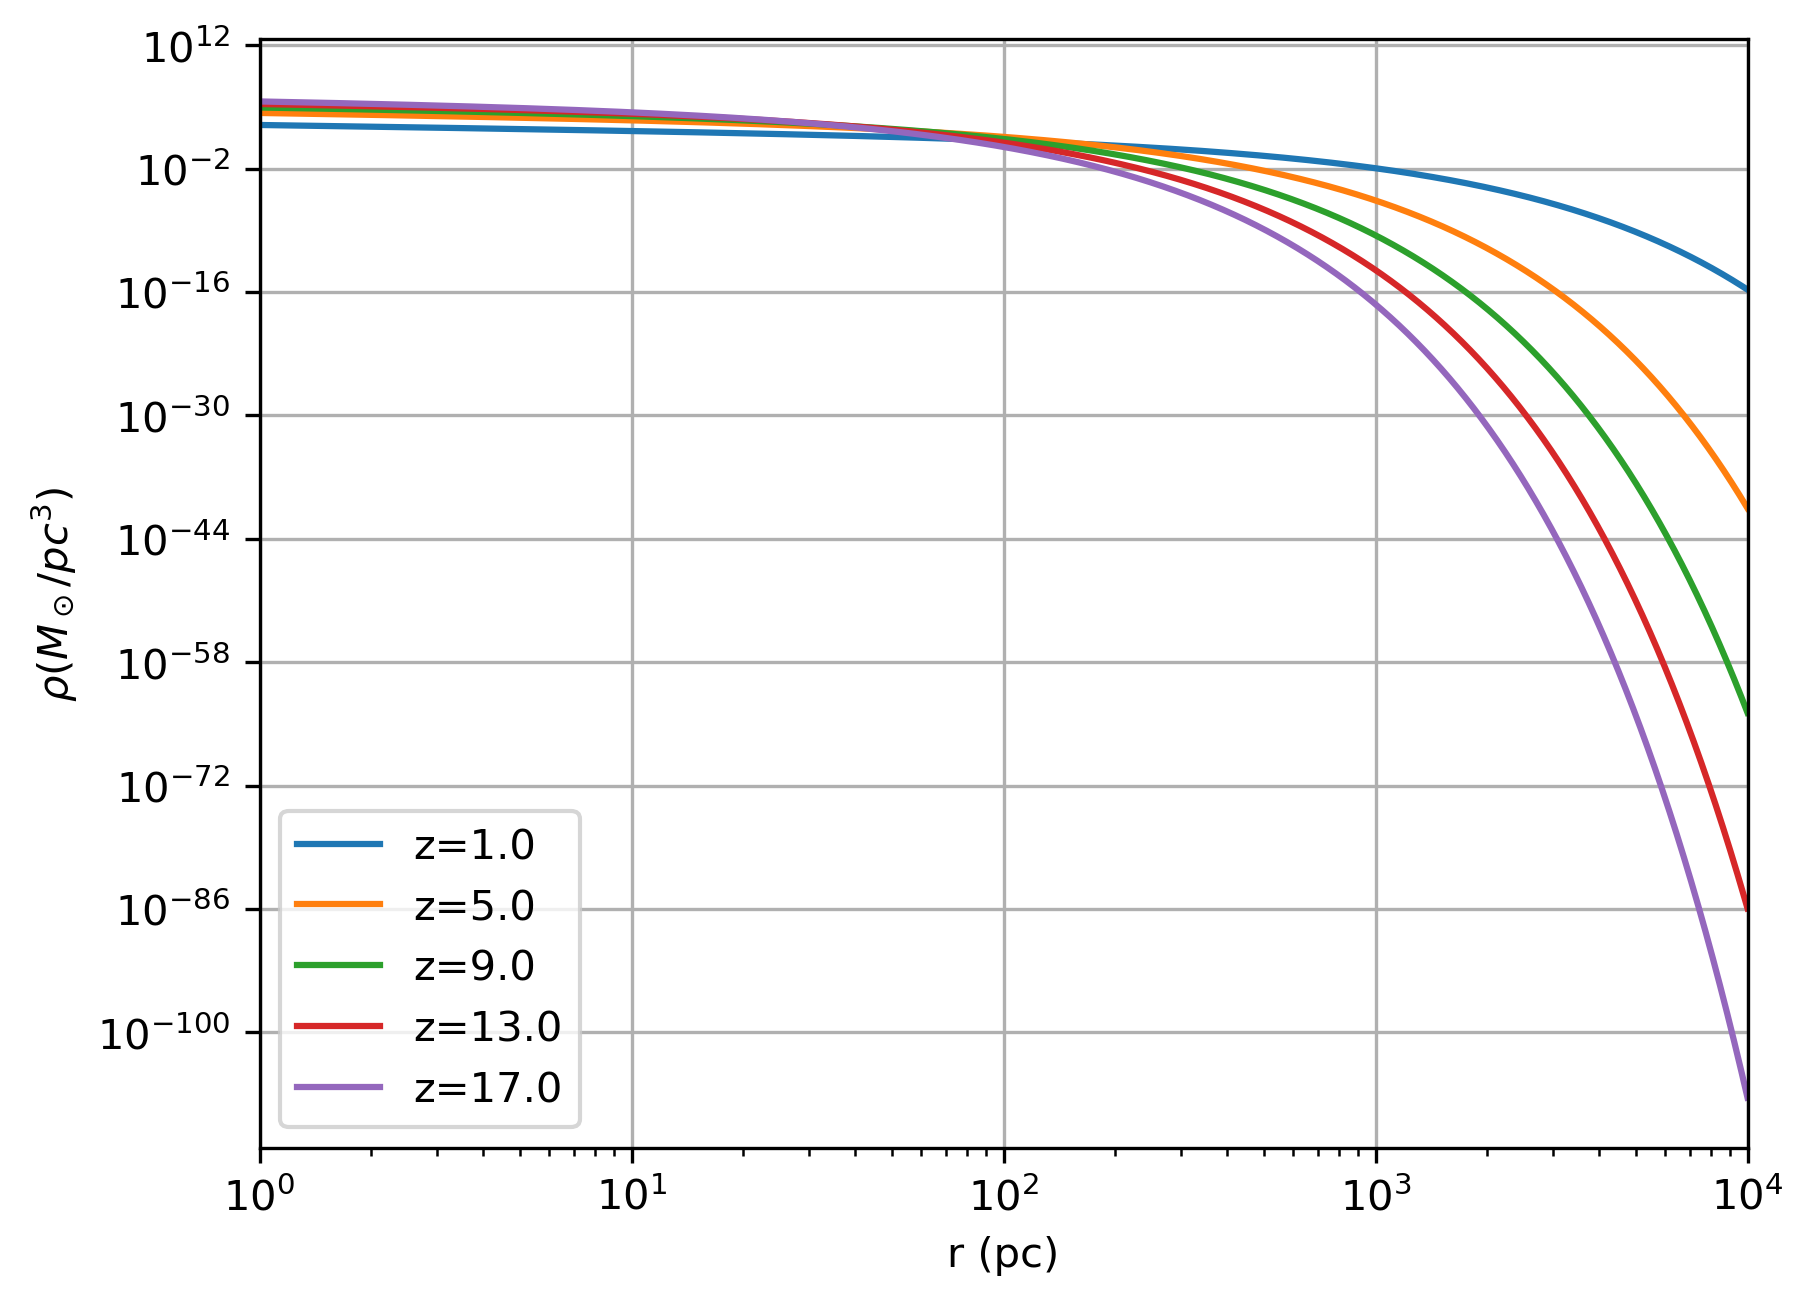
\includegraphics[width=0.5\linewidth]{Galaxies_density_profile.png}
    \caption{}
    \label{Cosmic size density plot}
\end{figure}
High redshift galaxies tend to be more compact than low redshift counterparts.\\Hardening radii are easly derived from these profiles according to Equation \ref{a_h dynamical definition} and a comparison between different hosts H and K functions- see Figure \ref{Cosmic size H plot} and \ref{Cosmic size K plot}- suggest that IMBH binary becomes "hard" at lower separation if embedded in a denser environment.
\begin{figure}[H]
    \centering
    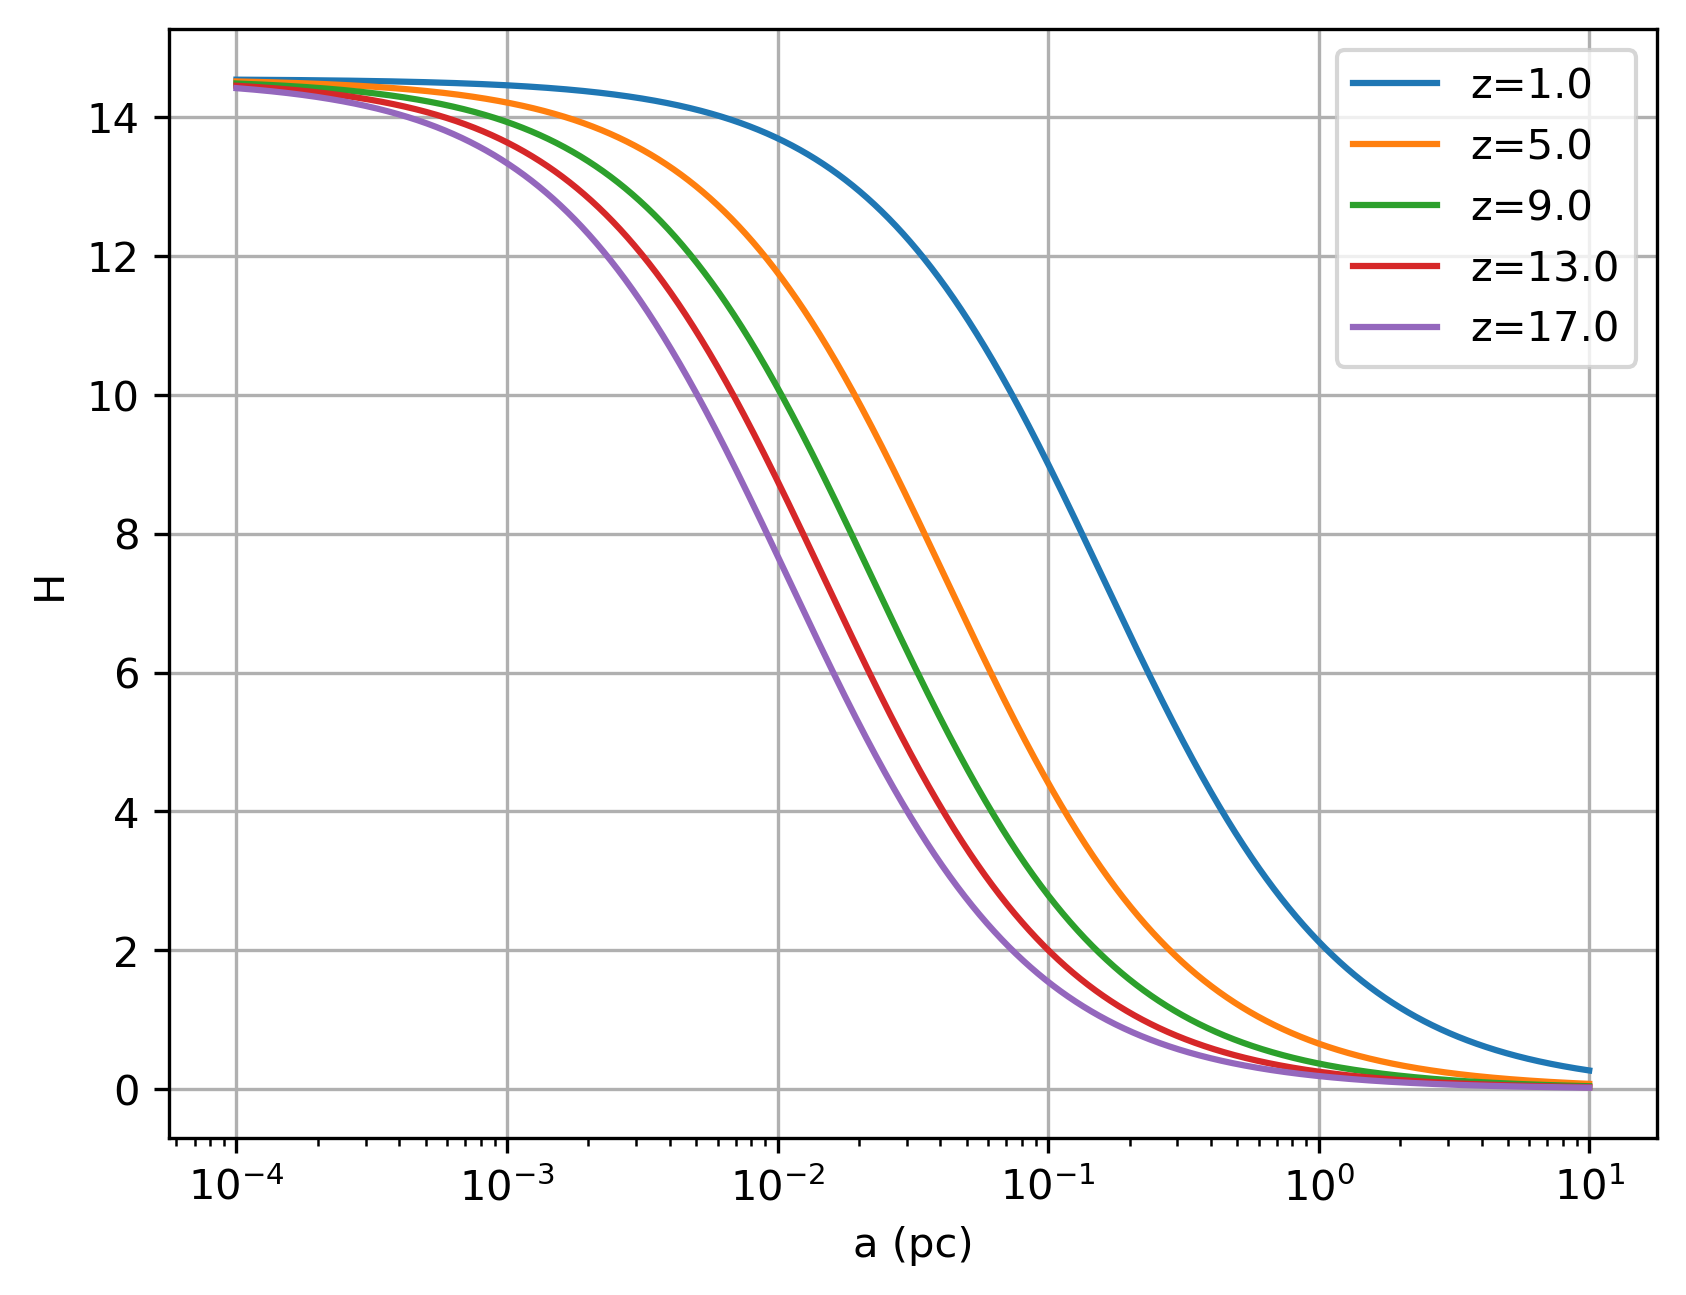
\includegraphics[width=0.5\linewidth]{Galaxies_H_unbound.png}
    \caption{}
    \label{Cosmic size H plot}
\end{figure}


\begin{figure}[H]
    \centering
    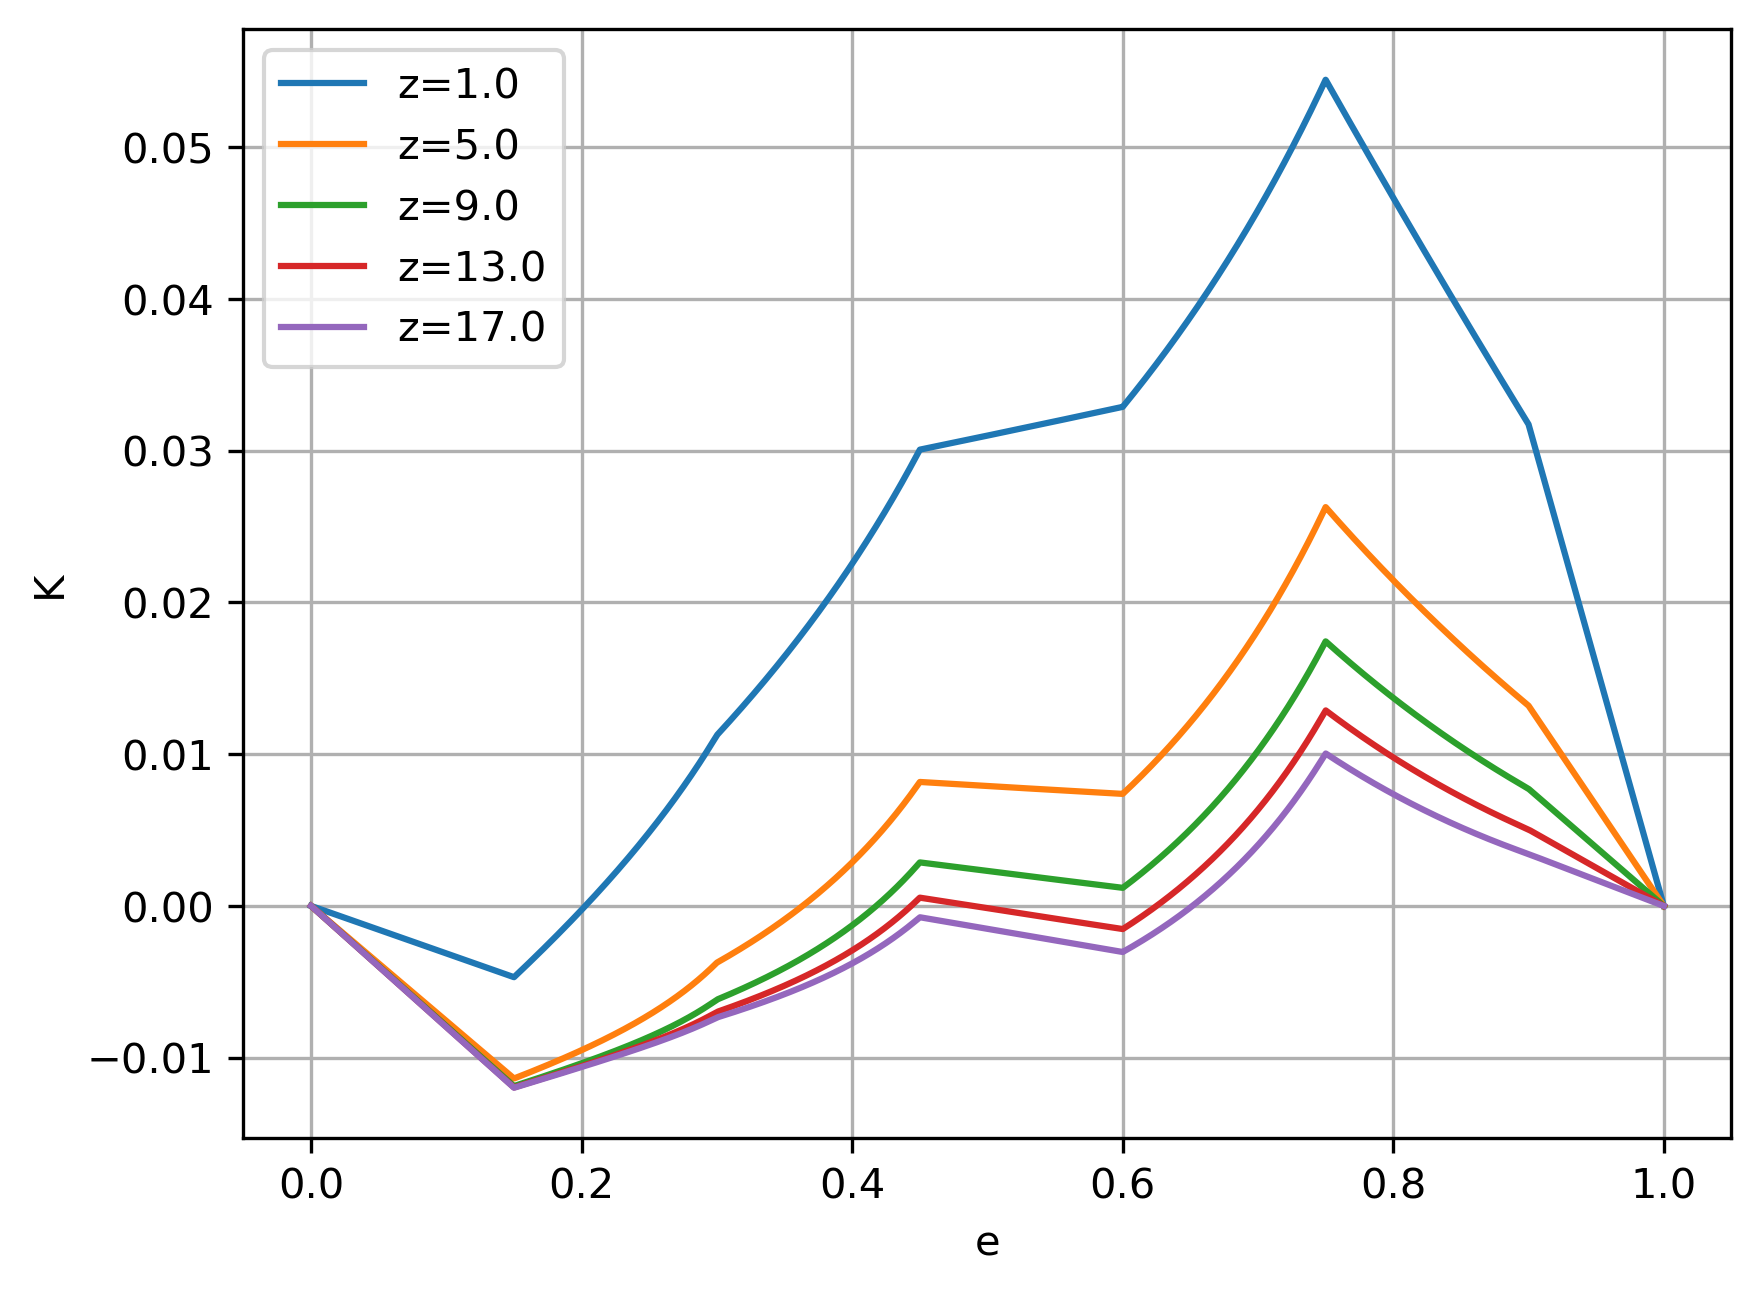
\includegraphics[width=0.5\linewidth]{Galaxies_K_unbound.png}
    \caption{This family of functions is obtained evaluating $K(a,e)$ of each galaxy at their mean hardening radius.}
    \label{Cosmic size K plot}
\end{figure}
We present in Figure \ref{Cosmic size a vs t plot} and \ref{Cosmic size e vs t plot} the evolutionary tracks of a sample of galaxies obtained by applying RK(4) to the Equations (\ref{da/dt Un+GW}) and (\ref{de/dt Un+GW}) and initial condition $(t_,a_0,e_0)=(0yr,15pc,0.7)$.
\begin{figure}[H]
    \centering
    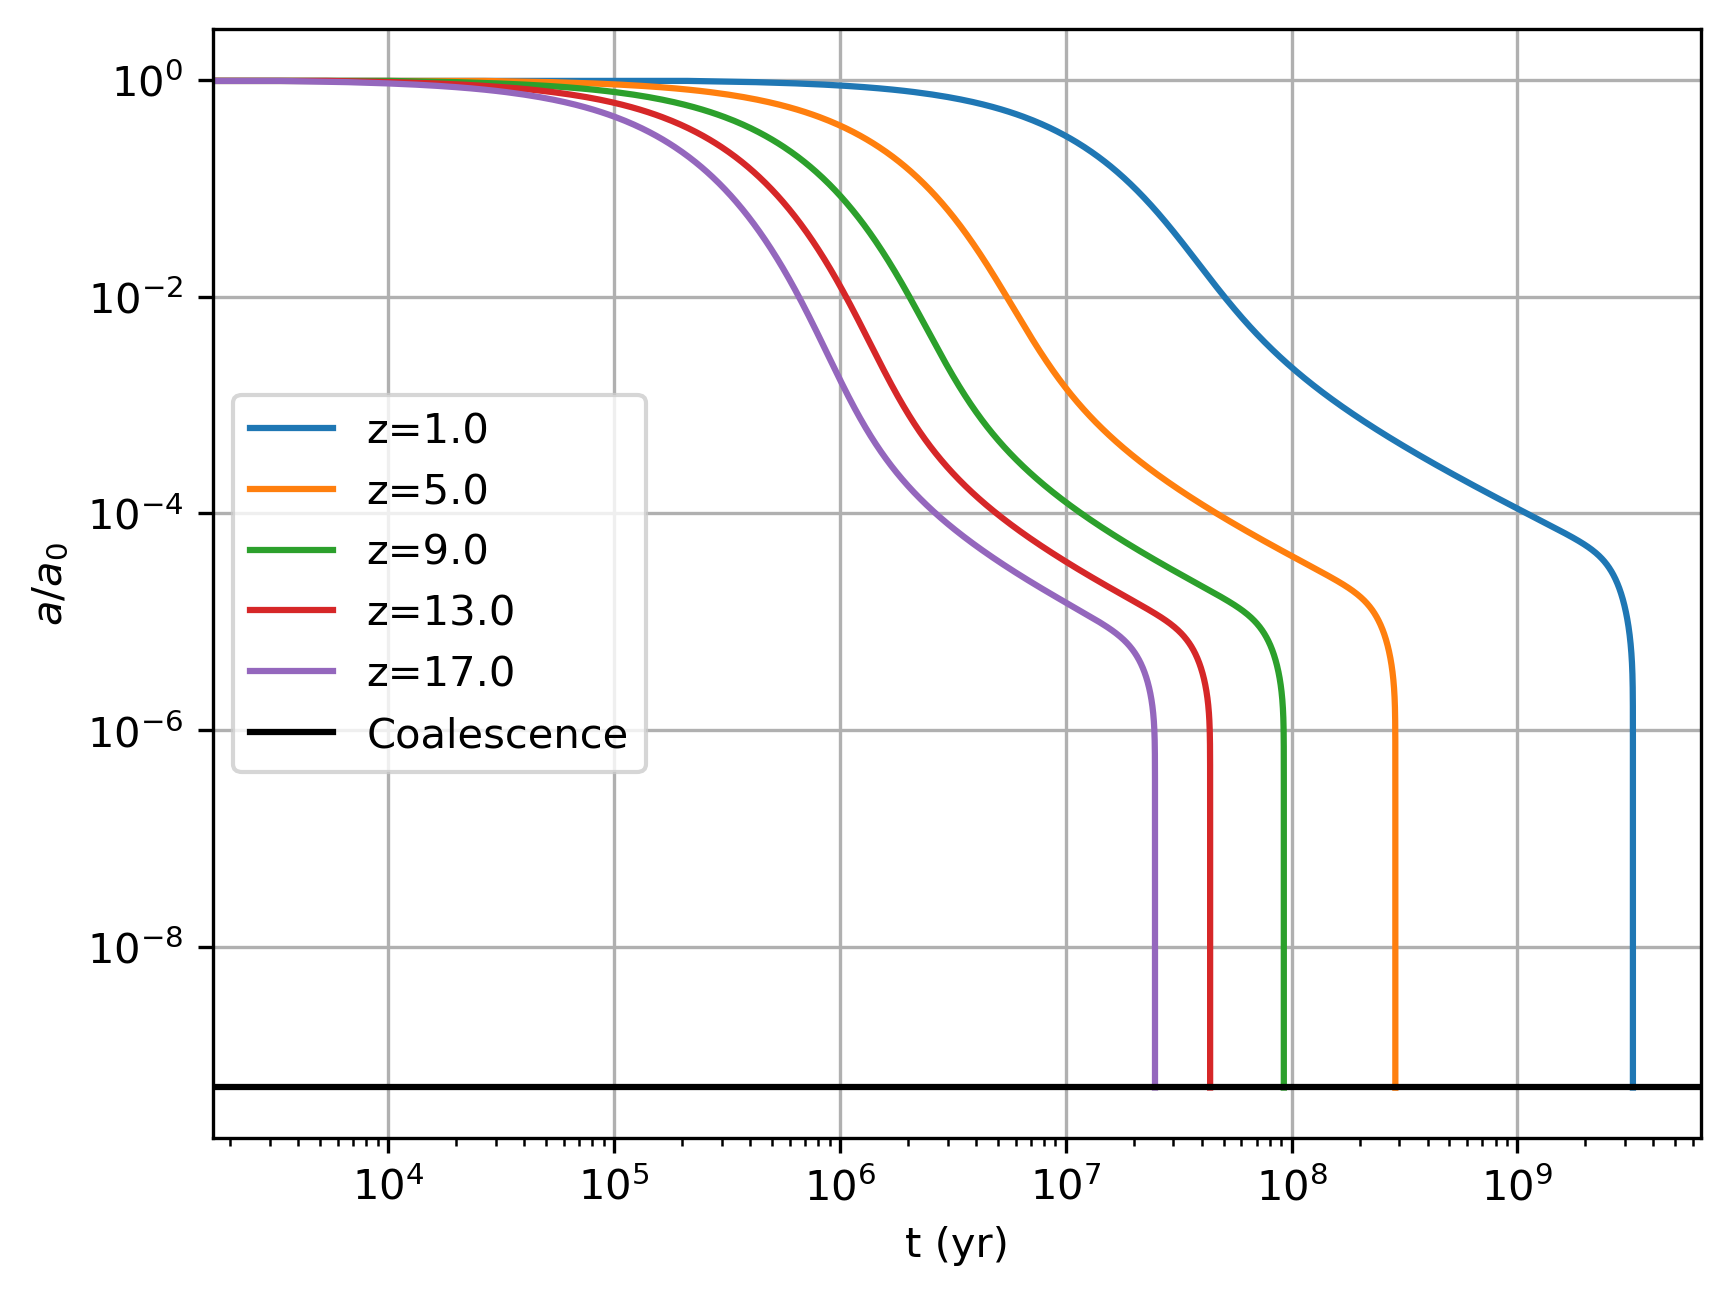
\includegraphics[width=0.5\linewidth]{Galaxies_a_vs_t.png}
    \caption{}
    \label{Cosmic size a vs t plot}
\end{figure}



\begin{figure}[H]
    \centering
    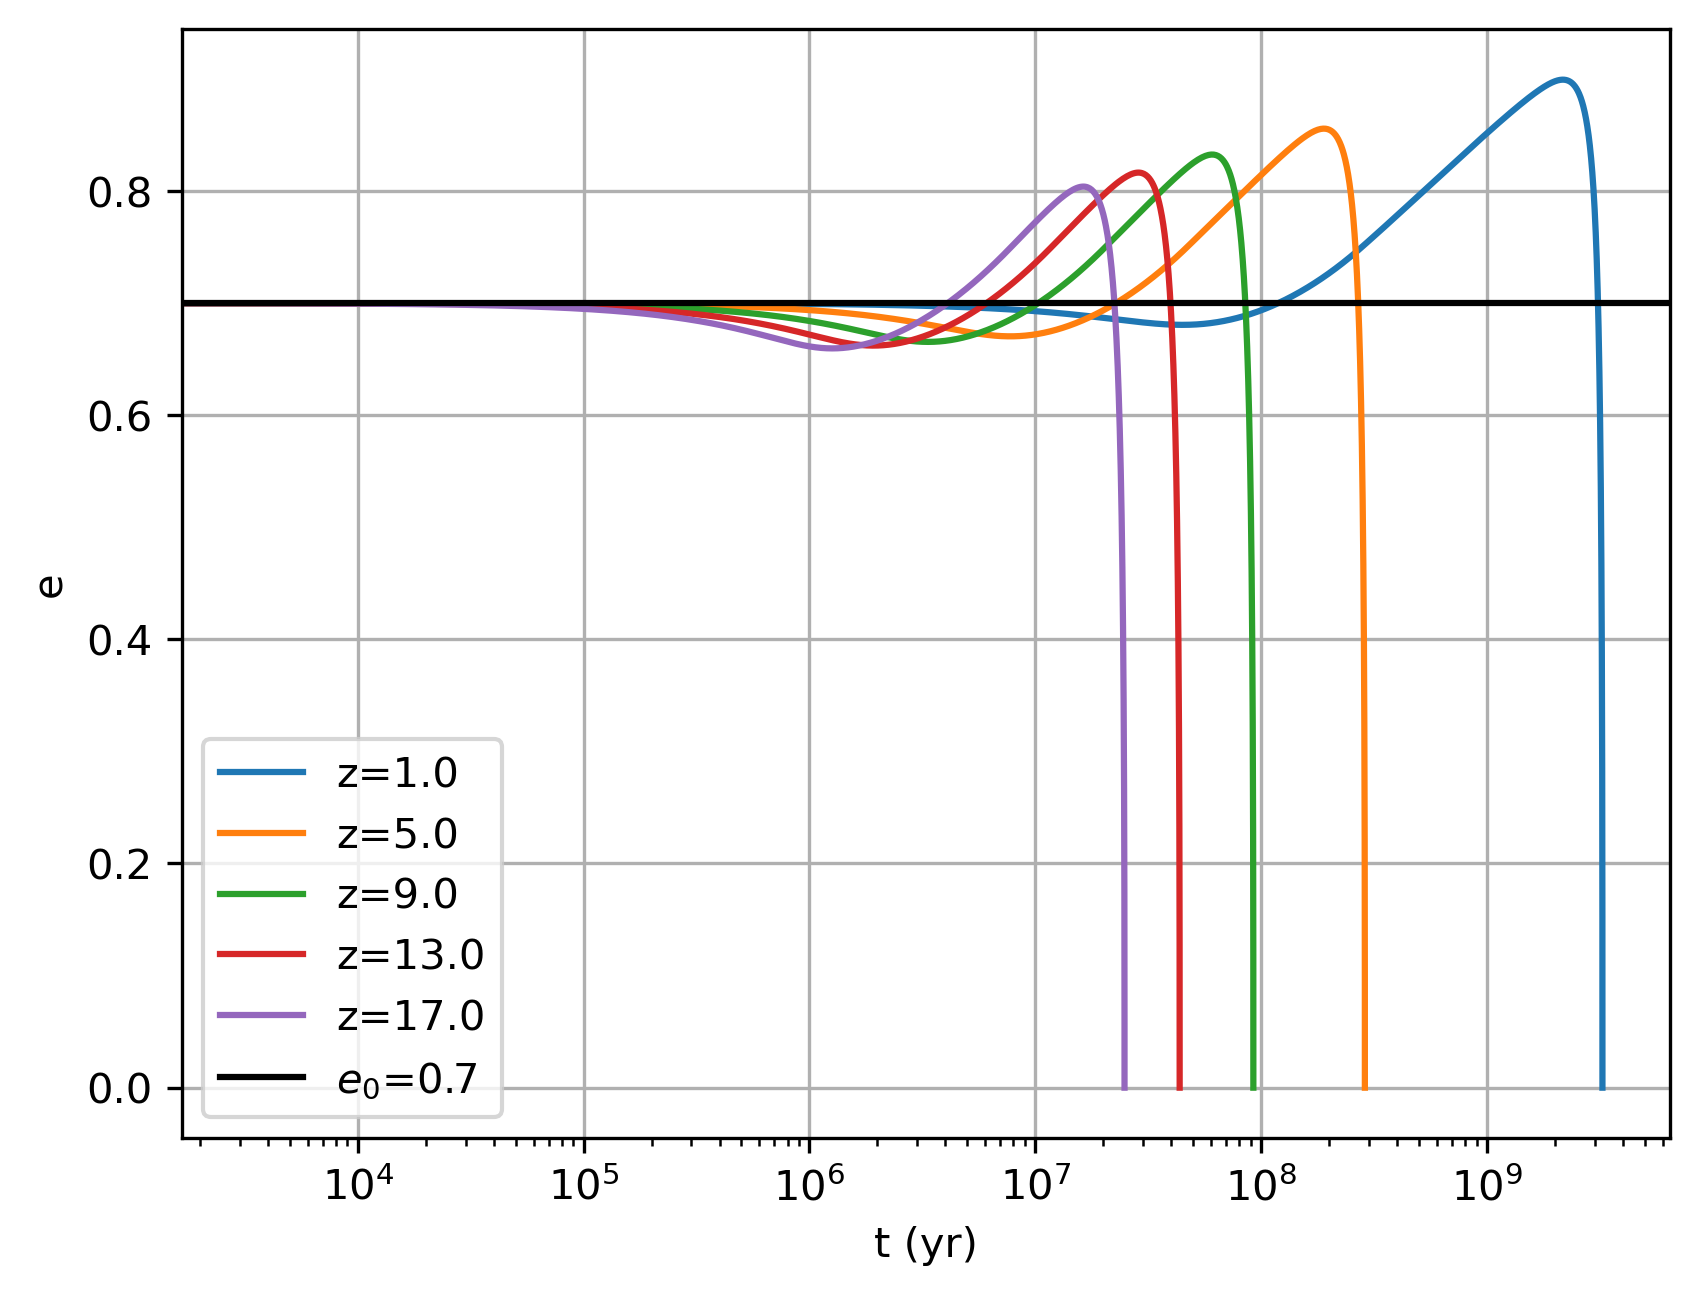
\includegraphics[width=0.5\linewidth]{Galaxies_e_vs_t.png}
    \caption{}
    \label{Cosmic size e vs t plot}
\end{figure}


\begin{table}[htbp]
\centering
\caption{Galaxies coalescence time grid (Gyr)}
\label{tab:example}
\begin{tabular}{ll}
\toprule
z & $t_{coal}$ (Gyr) \\
\midrule
 1  &  3.24728387   \\
 2  &  1.334011  \\
 3  &  0.7072763  \\
 4  &  0.43164087  \\
 5  &  0.28805534  \\
 6  &  0.20450559  \\
 7  &  0.15193439  \\
 8  &  0.11686942  \\
 9  &  0.09240003  \\
 10 &  0.07469761 \\
 11 &  0.06150781 \\
 12 &  0.05143637 \\
 13 &  0.04358488 \\
 14 &  0.03735426 \\
 15 &  0.03233322 \\
 16 &  0.02823207 \\
 17 &  0.02484224 \\
 18 &  0.02201059 \\
 19 &  0.01962278 \\
 20 &  0.01759202 \\
\bottomrule
\end{tabular}
\end{table}
We note that higher compactness tends to compensate the effects of NSC removal in terms of the coalescence time.\\Lastly, we modifiy the initial time $t_0$ of each run, turning it into $t(z)$, thus focusing on the possibility of coalescence within the present time and consequently a potential GWs observation.
\begin{figure}[H]
    \centering
    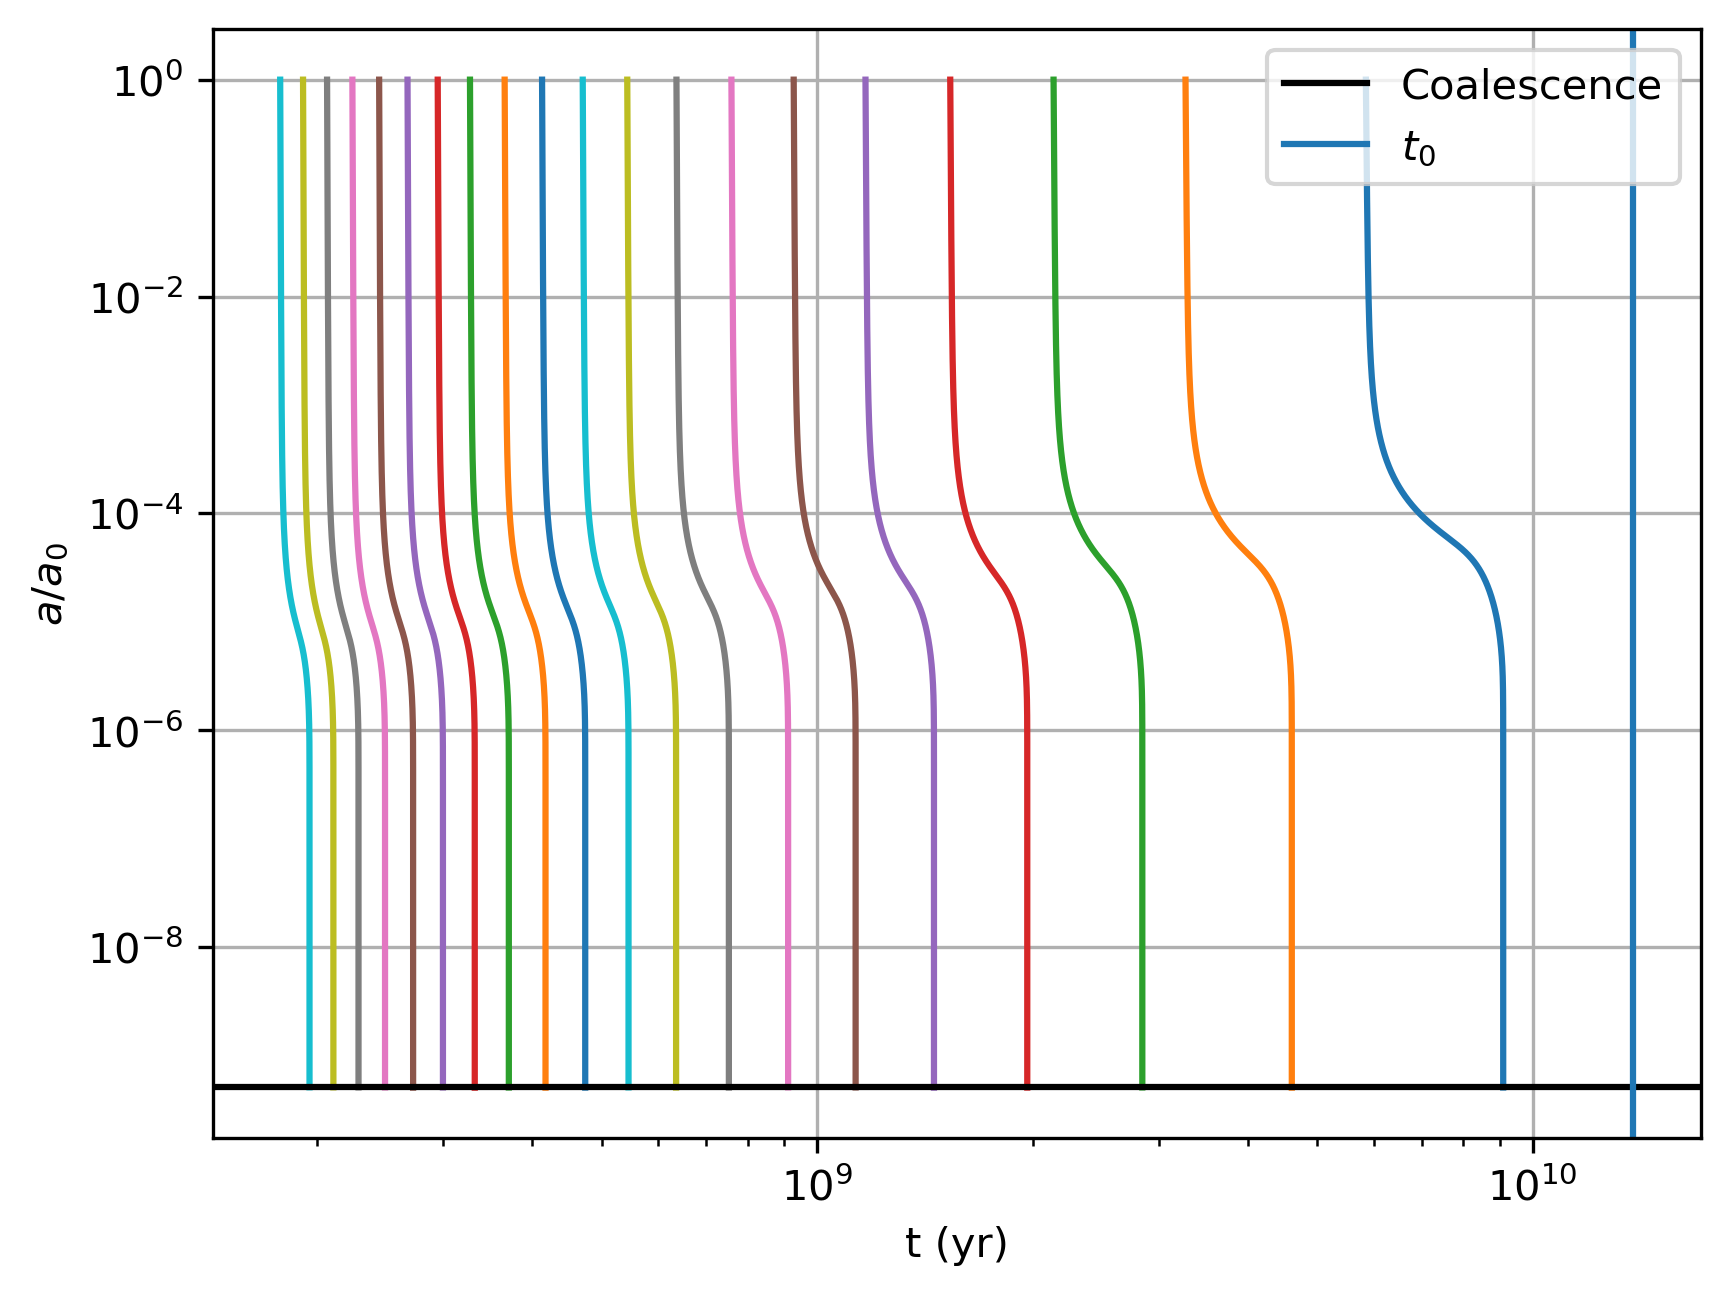
\includegraphics[width=0.5\linewidth]{Galaxies_a_vs_t_from_t(z).png}
    \caption{}
    \label{Cosmic size a vs t from t(z) plot}
\end{figure}
 
Therefore, forming in tha past at $z>0$, they all merge before the present time.















\section{N-body}

Within $t_{2b}$, usually much shorter than the age of the universe for common galaxies, 
granularity is unimportant, collisions are negligible and stars can be described as
 particles moving in a smooth potential
generated by a continous $\rho$. Hence, stars will have a DF satisfying the CBE: 

\begin{equation}\label{CBE}
    \frac{Df}{Dt}=\frac{\partial f}{\partial t}+
    \mathbf{\dot{w}}\cdot \frac{\partial f}{\partial \mathbf{w}}=
    \frac{\partial f}{\partial t}+[f,H]=0
\end{equation}



In cartesian coordinates the Hamiltonian is
\begin{equation}\label{Hamiltonian in cartesian coord.}
    H(\mathbf{x},\mathbf{v})=\frac{1}{2}v^2+\Phi(\mathbf{x})
\end{equation}

and the CBE becomes

\begin{equation}\label{CBE in cartesian coord.}
    0=\frac{\partial f}{\partial t}+\mathbf{v}\cdot 
    \frac{\partial f}{\partial \mathbf{x}}-
    \frac{\partial \Phi}{\partial \mathbf{x}}
    \cdot \frac{\partial f}{\partial \mathbf{v}}
\end{equation}

Several times beyond $t_{2b}$ the system enters the collisional regime and first order 
corrections to the CBE are needed; the Fokker-Planck equation is an example of this:
\begin{equation}
    \frac{Df}{Dt}=C[f]
\end{equation}
where simplifications on the collision operator $C[f]$ can be done.\\In this scenario $f$ is 
no longer conserved along the orbit of the potential $\Phi$ and diffusion in the PS occurs, 
both $E$ and $L$ of a single star can change due to collisions, at odds with the CBE regime 
where, for istance $DH/Dt=0$. It is used in the loss cone problem.\\In order to exploit the 
properties of the CBE it is usefull to introduce the velocity moments, which will appear 
inside the Jeans equations:
\begin{equation}
    \overline{v_i}(\mathbf{x},t)\equiv 
    \frac{1}{\rho(\mathbf{x},t)}\int_\mathcal{R}^3 d^3 \mathbf{v} f v_i
\end{equation}
\begin{equation}
    \sigma_{ij}^2(\mathbf{x},t)\equiv 
    \frac{1}{\rho(\mathbf{x},t)}\int_\mathcal{R}^3 d^3 \mathbf{v}
    f (v_i-\overline{v_i})(v_j-\overline{v_j})=\overline{v_iv_j}-
    \overline{v_i}\,\overline{v_j}
\end{equation}
A function $I(\mathbf{x},\mathbf{v})$
is an integral of motion if and only if
\begin{equation}\label{Integral of motion def}
    \frac{D}{Dt}[I(\mathbf{x}(t),\mathbf{v}(t))]=0
\end{equation}
along any orbit of the potential $\Phi$.
\\Jeans Theorem: 
Any steady-state solution of the collisionless Boltzmann equation depends on 
the phase-space coordinates only through integrals of motion in the given potential, and any 
function of the integrals yields a steady-state solution of the collisionless Boltzmann 
equation.\\In a steady-state potential the Hamiltonian is an integral of motion; therefore $f$
will be any non-negative function of $H$.
\\Ergodic DFs: they are of the kind $f=f(H)$.
\\Equilibrium stellar systems have $\overline{v_i}=0$ and isotropic velocity-dispersion tensor
(being symmetric it can be diagonalized at any point in a proper orthogonal set of axes), i.e 
$\sigma^2_{ij}=\sigma^2 \delta_{ij}$. Thus every system with an ergodic DF is isotropic.
\\If the potential $\Phi$ is time-indipendent and spherically symmetric, then $\mathbf{L}$ 
appears as three isolating integral of motions but DF will depend on them only through 
$|\mathbf{L}|=L$, i.e. $f=f(H,L)$.Adopting spherical coordinates and splitting 
$v^2=v_r^2+v_t^2$, it holds 
\begin{equation}
    \overline{v_r}=0
\end{equation}
\begin{equation}
    \overline{\mathbf{v_t}}=\mathbf{0}
\end{equation}
and in general $\sigma_{ij}$ is diagonal with $\sigma^2_r\ne \sigma^2_\theta=\sigma^2_\phi$.\\Recovering
the DF from $\rho$ can be done by Eddington's formula, which applies to spherically symmetric,
globally isotropic stellar systems,
\begin{equation}\label{Eddington's formula}
f(\varepsilon)=\frac{1}{\sqrt{8}\pi^2}\frac{d}{d\varepsilon}
\int_{\varepsilon_t}^{\varepsilon}
\frac{d\rho}{d\Psi}\frac{d\Psi}{\sqrt{\varepsilon-\Psi}}
\end{equation}
with $\varepsilon=-H$ and $\Psi=-\Phi$ being the relative energy and potential respectively
and $\varepsilon_t$ the truncation energy of the system.\\Given the density profile, IC for N-body
simulations are generated by OpOpgadget software by sampling uniformly the internal mass profile
and the potential produced by the smooth profile $\rho$.\\The Sersic profile introduced by 
\textcite{Prugniel} has (with standard substitution $Z=b\left(\frac{r}{R_e}\right)^{1/n}$)
\begin{equation}\label{Sersic mass profile}
    M(<r)=4\pi \rho_0 R_e^3 n b^{n(p-3)}\gamma\left[n(3-p),b\left(\frac{r}{R_e}\right)^
    {1/n}\right]=M_*\frac{\gamma\left[n(3-p),b\left(\frac{r}{R_e}\right)^
    {1/n}\right]}{\Gamma[n(3-p)]}
\end{equation}
with 
\begin{equation}\label{complete gamma fun}
    \Gamma(a)=\int_{0}^{\infty}dt e^{-t}t^{a-1}
\end{equation}
the "Complete gamma function", 
\begin{equation}\label{upper incomplete gamma fun}
    \Gamma(a,x)=\int_{x}^{\infty}dt\,e^{-t}t^{a-1}
\end{equation}
the Upper incomplete gamma function and
\begin{equation}\label{lower incomplete gamma fun}
    \gamma(a,x)=\int_{0}^{x}dt\,e^{-t}t^{a-1}
\end{equation}
the Lower incomplete gamma function. By definition follows:
\begin{equation}\label{gamma fun relation}
    \Gamma(a)=\Gamma(a,x)+\gamma(a,x)
\end{equation}
The spatial distribution is spherical and untruncated but the mass profile converges to 
the finite value $M_*$, so the potential can be found from
\begin{equation}\label{spherical potential, general formula}
    \Phi(r)=\Phi(r_0)+\frac{GM(<r_0)}{r_0}-\frac{GM(<r)}{r}-4\pi G \int_{r}^{r_0}dt\,t \rho(t)
\end{equation}
Setting $r_0\rightarrow \infty$ and $\Phi(r_0)=0$, it becomes
\begin{equation}\label{spherical potential, simplified formula}
    \Phi(r)=-\frac{GM(<r)}{r}-4\pi G \int_{r}^{\infty}dt\,t \rho(t)
\end{equation}
and computation returns
\begin{equation}
\Phi(r)=
-4\pi G \rho_0 R_e^2 n\, b^{\,n(p-2)}
\left\{
\frac{b^{-n}}{r/R_e}\,
\gamma\!\left[n(3-p),Z\right]
+
\Gamma\!\left[n(2-p),Z\right]
\right\}
\end{equation}
or equivalently
\begin{equation}
    \Phi(r)=-\frac{GM_*}{r}\left\{\frac{\gamma\!\left[n(3-p),Z\right]}{\Gamma[n(3-p)]
    }+Z^n\frac{\Gamma[n(2-p),Z]}{\Gamma[n(3-p)]}\right\}
\end{equation}
The generation of IC for the dwarf galaxy NGC 2O5, hereafter taken as a $z=0$ nucleated dwarf
galaxy, is carried by OpOpgadget; the Sersic profile defined in this software is based on the 
one analyzed by \textcite{Neto_1999}, i.e.
\begin{equation}\label{Sersic profile Neto}
    \rho(r)=\rho_0\left(\frac{r}{a}\right)^{-p}e^{-(r/a)^\nu},
\end{equation}
where $n=\nu^{-1}$, $a$ is the Sersic profile scalelength and no $b(n)$ is present. The same
model can be described through several combinations of indipendent parameters; here, in order 
to use the effective radii values obtained from sky survy, we need to use the analytical
approximation 
\begin{equation}
    \ln{R_{eff}/a}=\frac{0.6950-\ln{\nu}}{\nu}-0.1789
\end{equation}

\begin{figure}
    \centering
    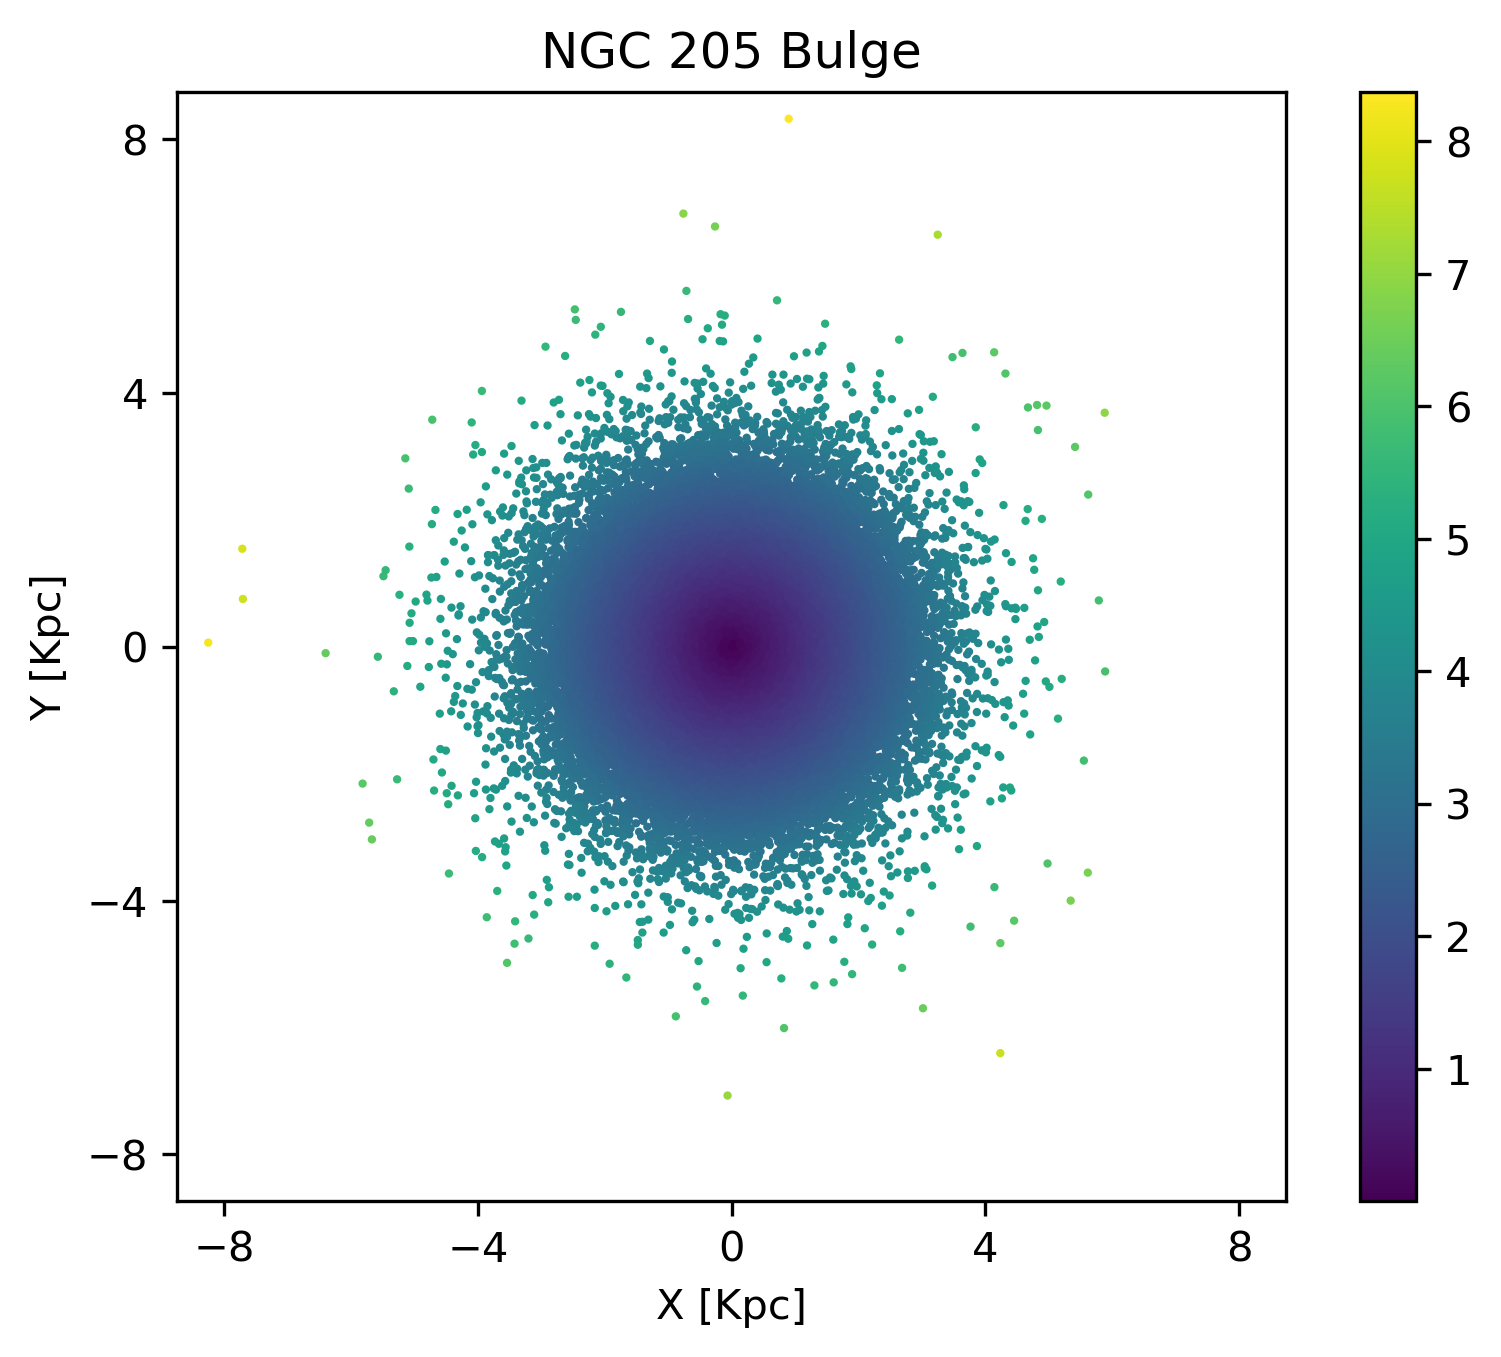
\includegraphics[width=0.5\linewidth]{NGC205_bulge_scatter.png}
    \caption{aaa}
    \label{NGC205_bulge_scatter}
\end{figure}

\begin{figure}
    \centering
    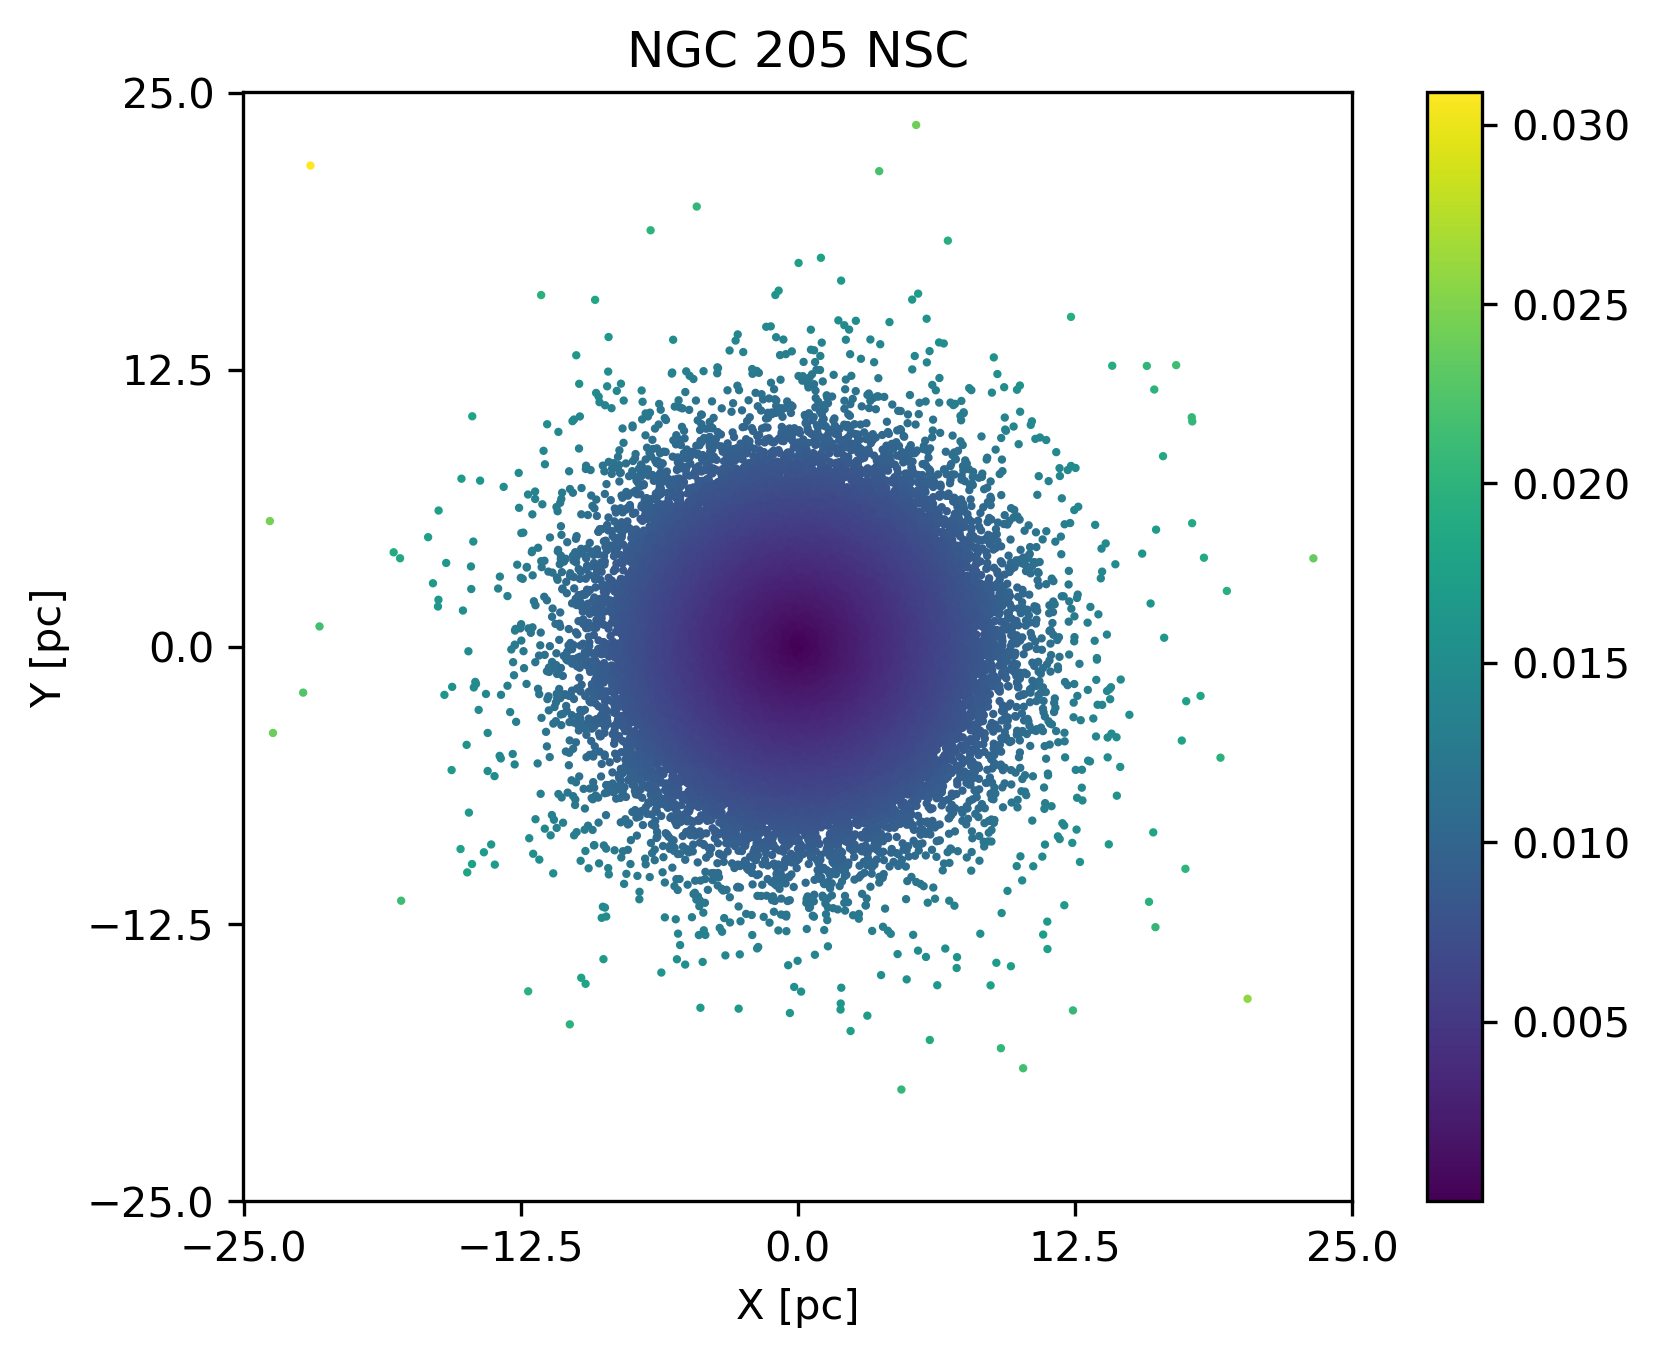
\includegraphics[width=0.5\linewidth]{NGC205_NSC_scatter.png}
    \caption{aaa}
    \label{NGC205_NSC_scatter}
\end{figure}

\begin{figure}
    \centering
    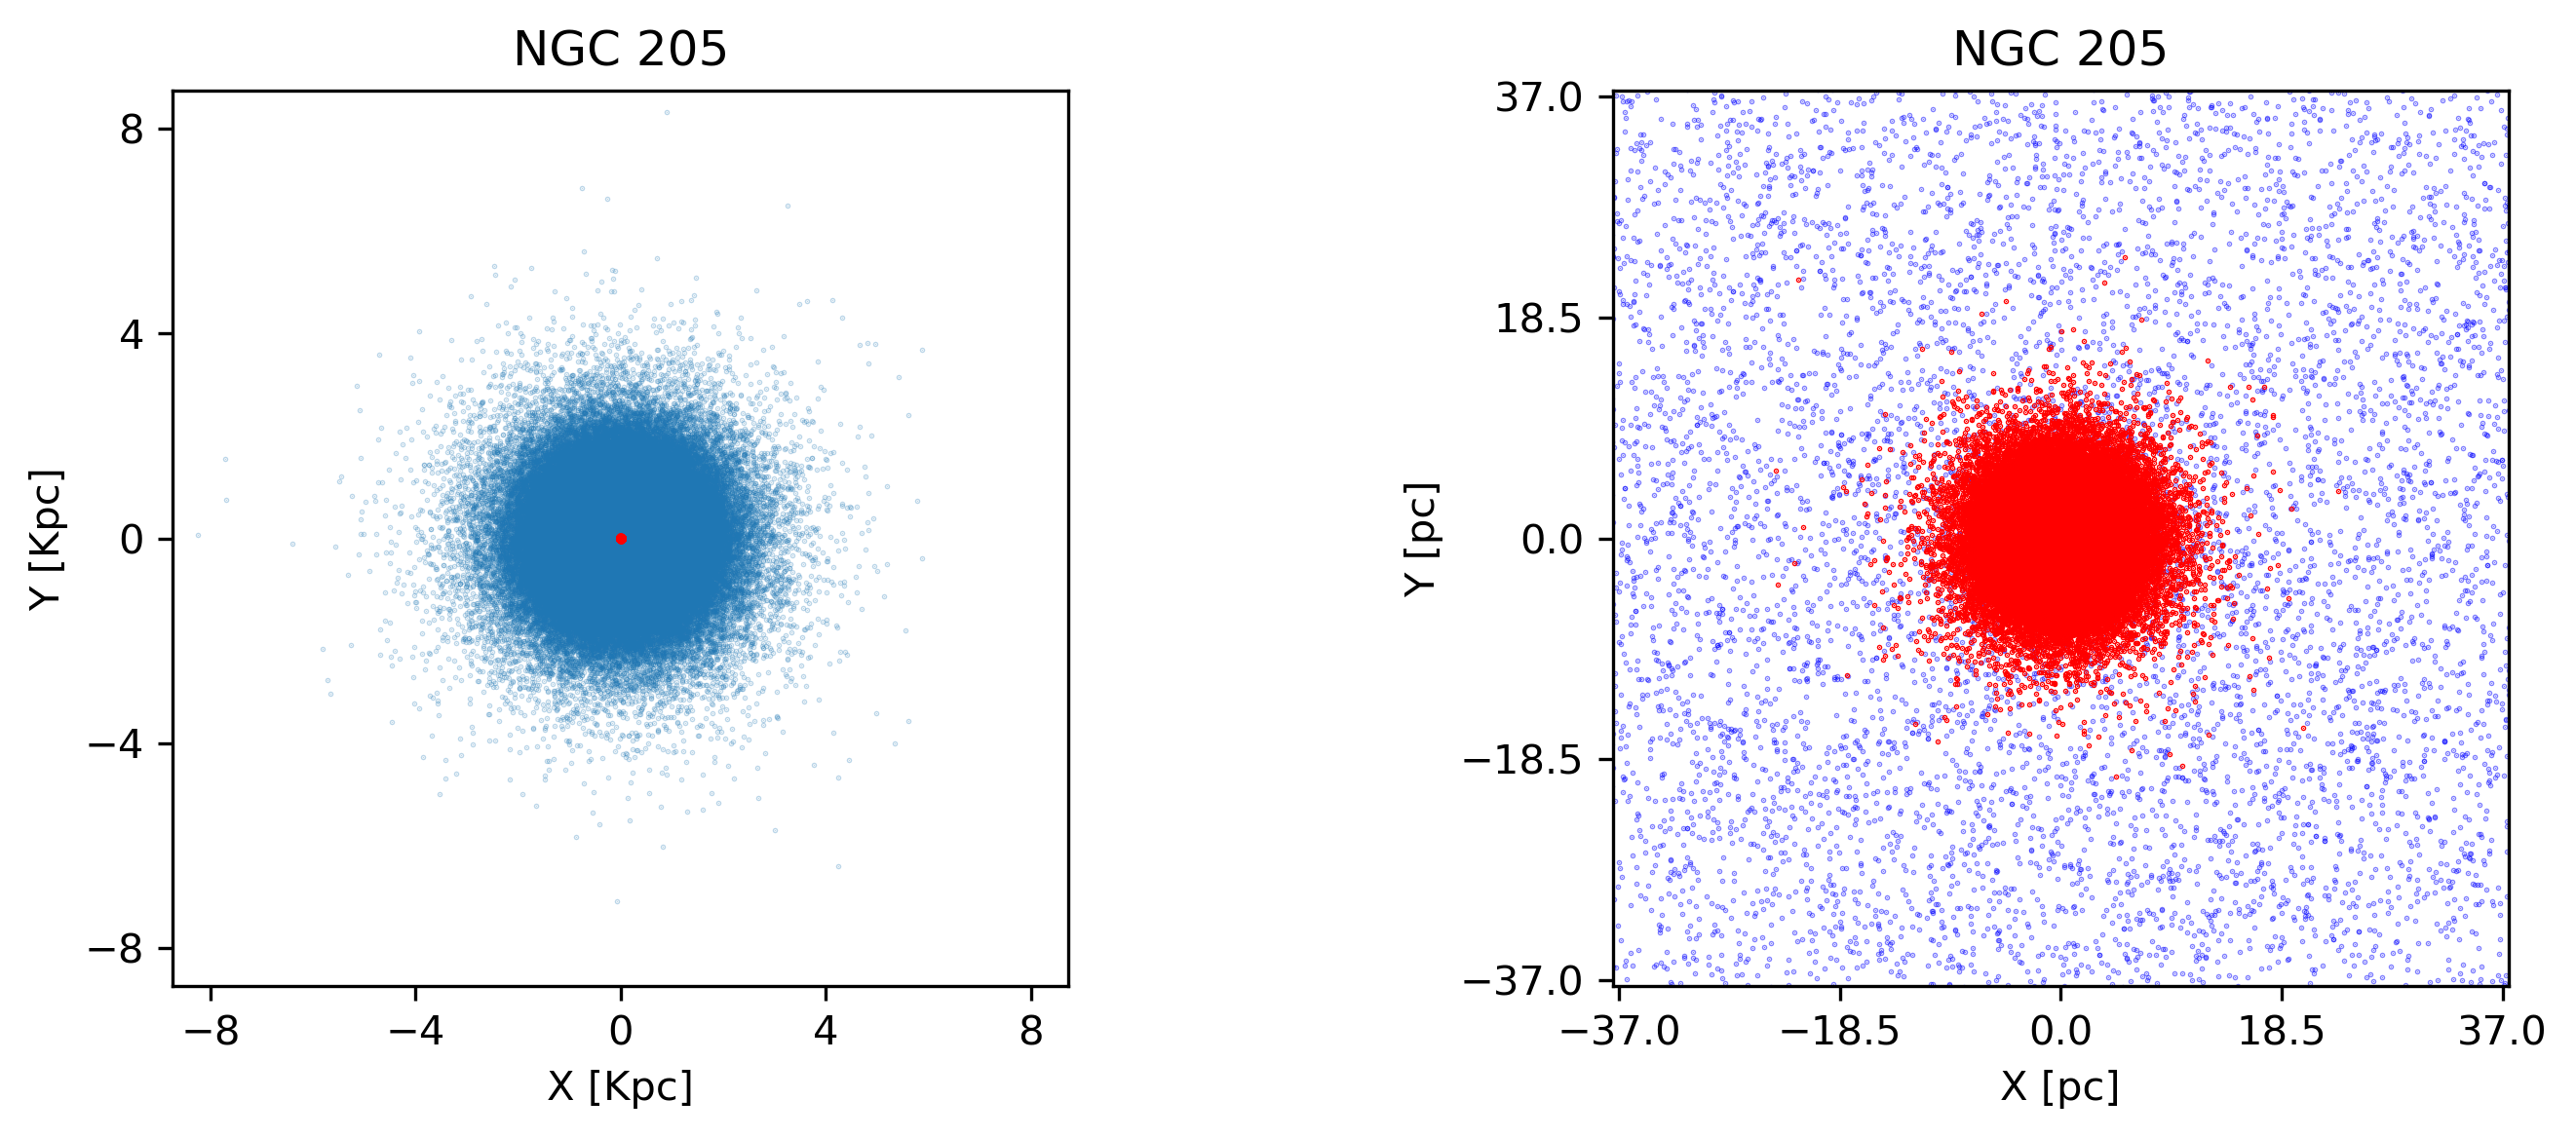
\includegraphics[width=0.5\linewidth]{NGC205_scatter.png}
    \caption{aaa}
    \label{NGC205_scatter}
\end{figure}


\begin{figure}[h]
\centering
 \begin{subfigure}{0.3\textwidth}
        \centering
        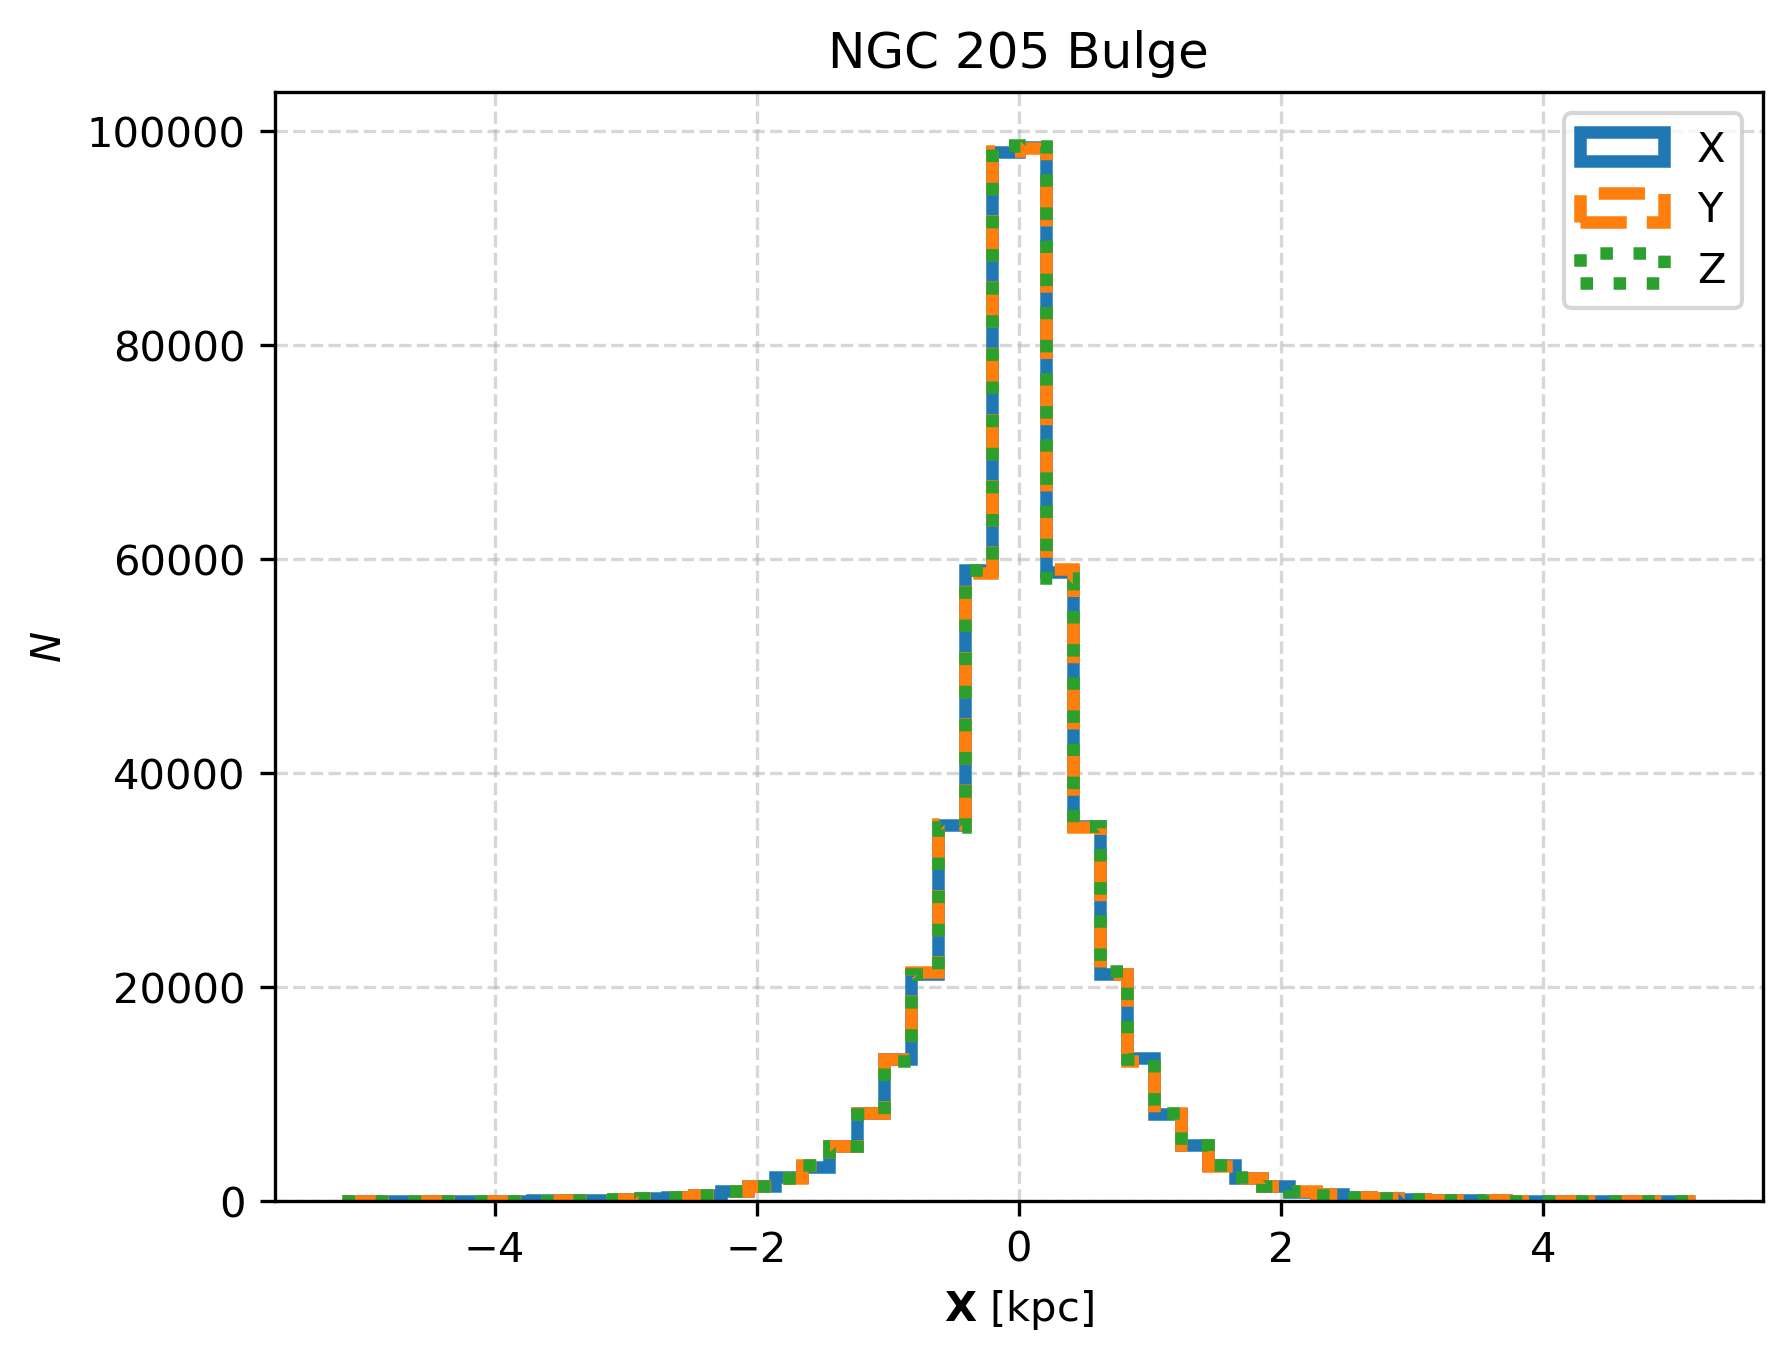
\includegraphics[width=\linewidth]{NGC205_bulge_space_hist.png}
        \caption{A}
    \end{subfigure}
    \hfill
    \begin{subfigure}{0.3\textwidth}
        \centering
        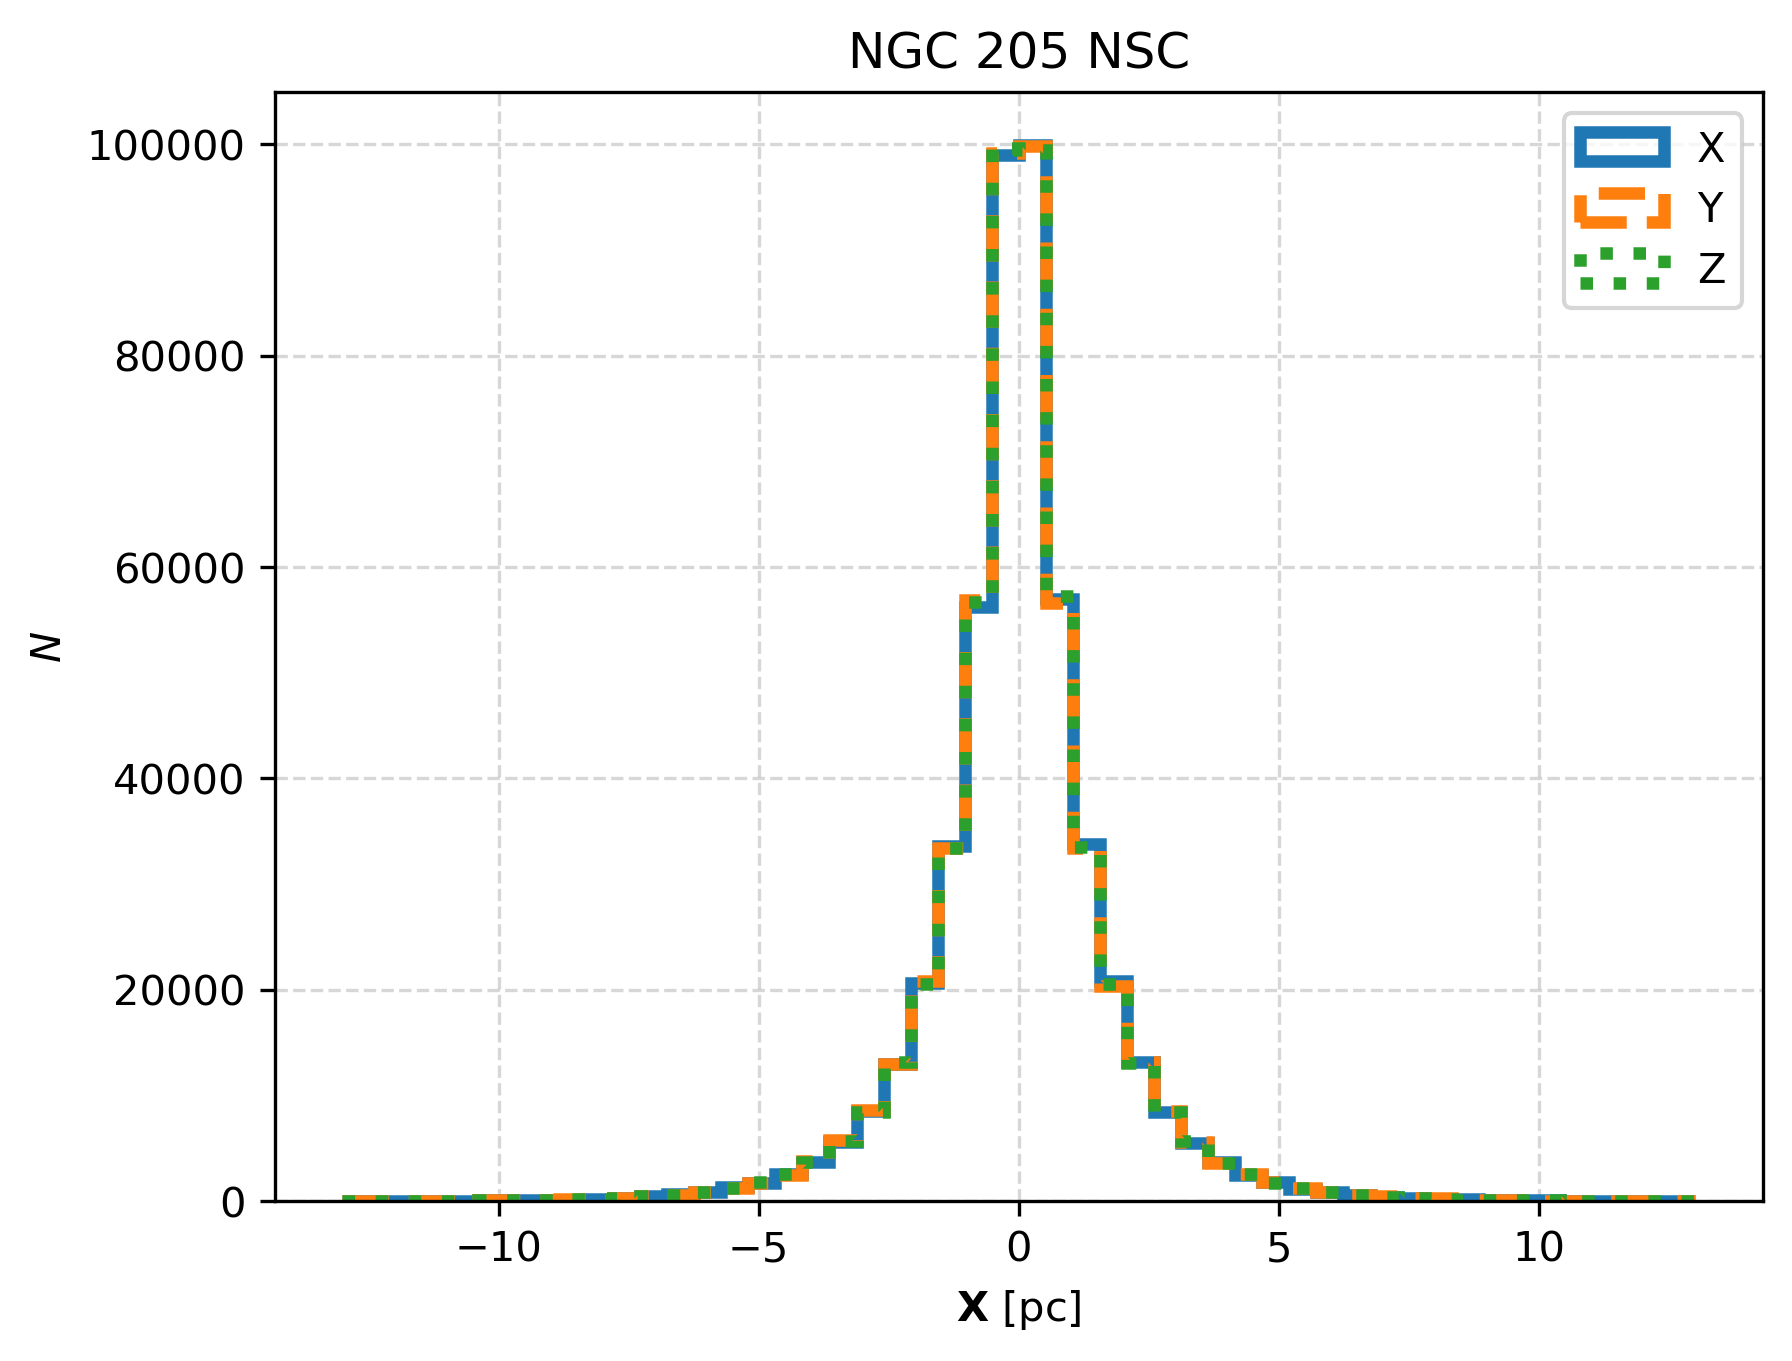
\includegraphics[width=\linewidth]{NGC205_NSC_space_hist.png}
        \caption{B}
    \end{subfigure}
    \hfill
    \begin{subfigure}{0.3\textwidth}
        \centering
        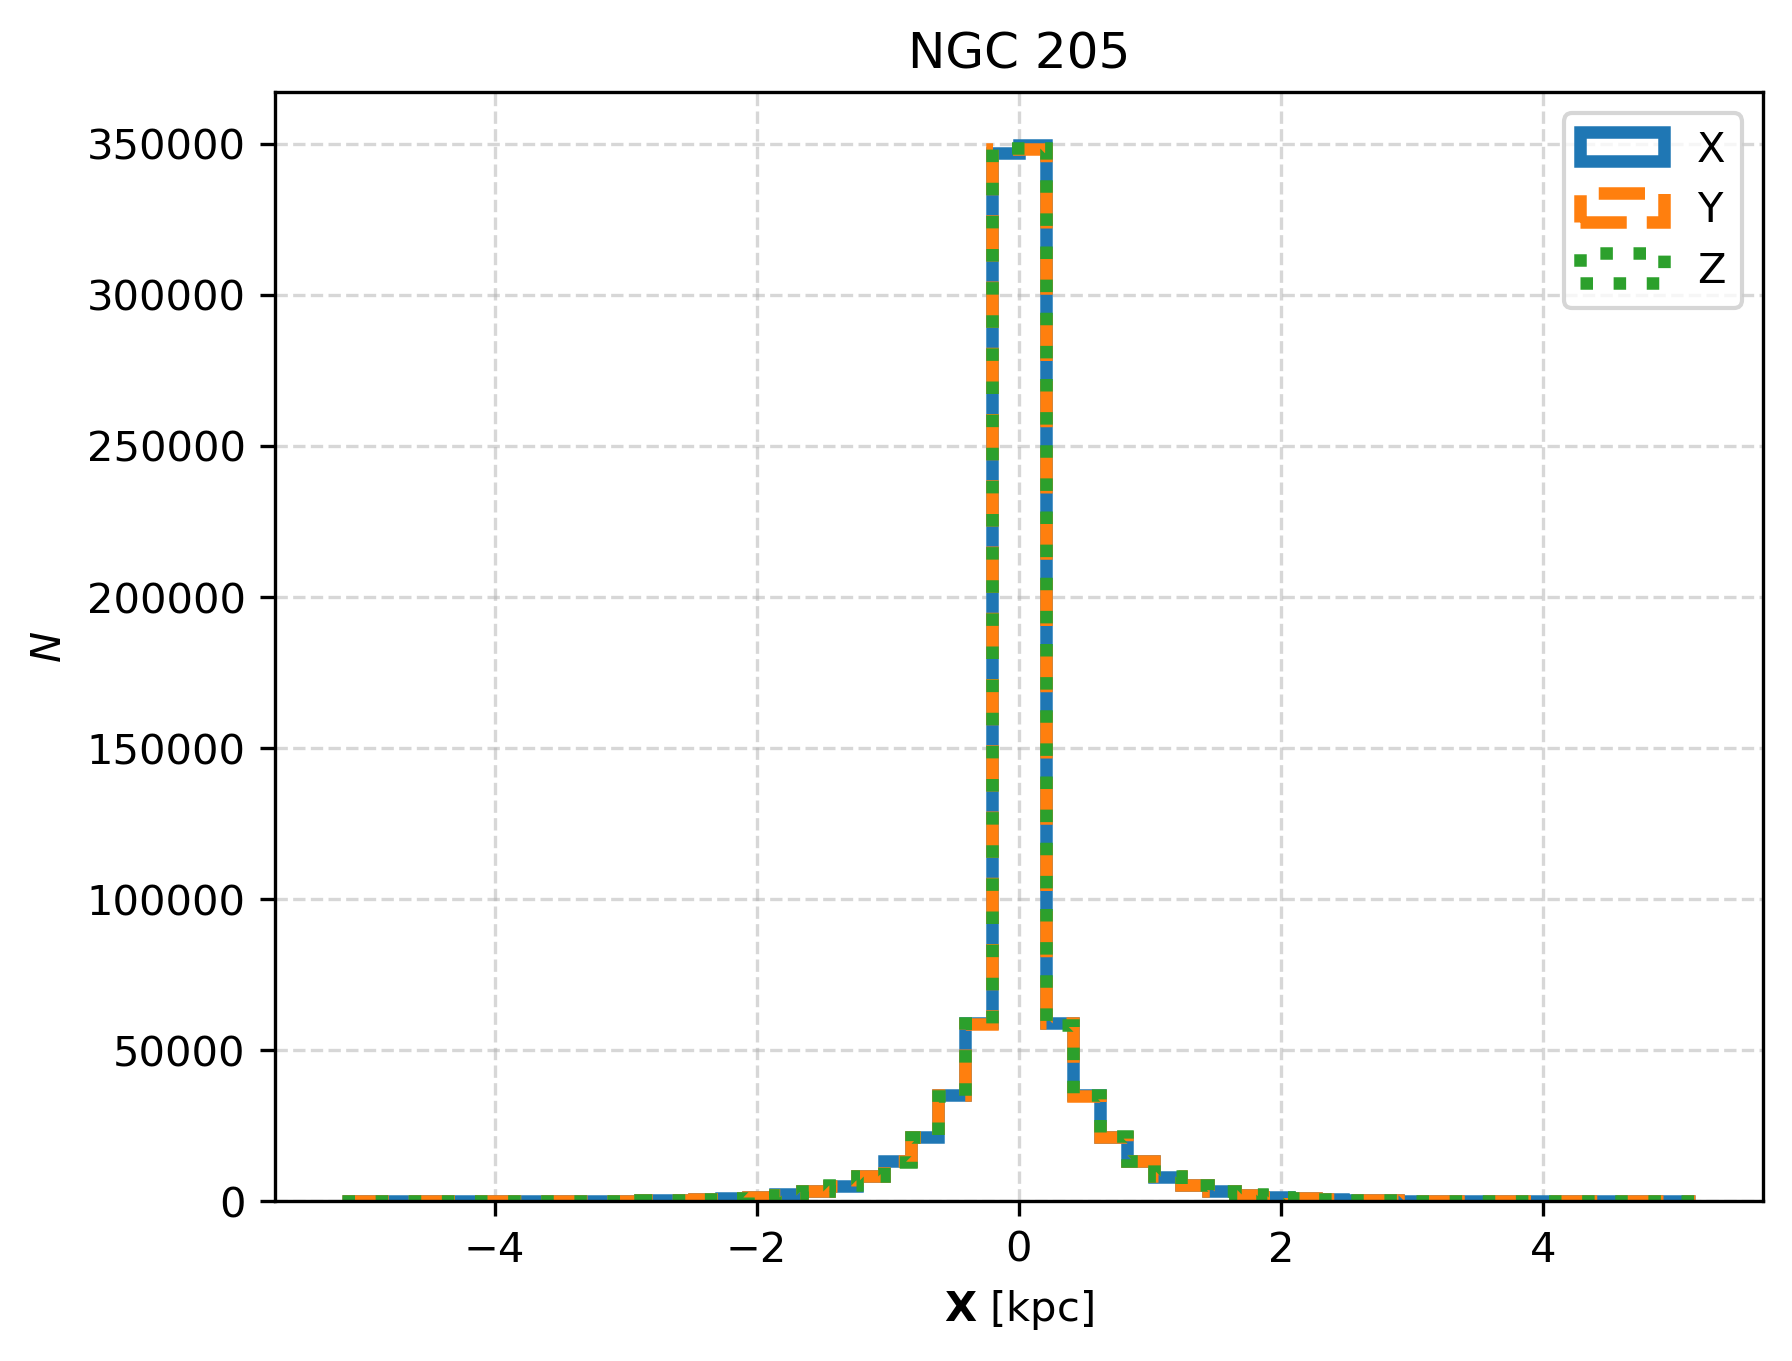
\includegraphics[width=\linewidth]{NGC205_space_hist.png}
        \caption{C}
    \end{subfigure}
    
    \caption{aaa}
    \label{3 NGC205_space_hist}
\end{figure}

\begin{figure}[h]
\centering
 \begin{subfigure}{0.3\textwidth}
        \centering
        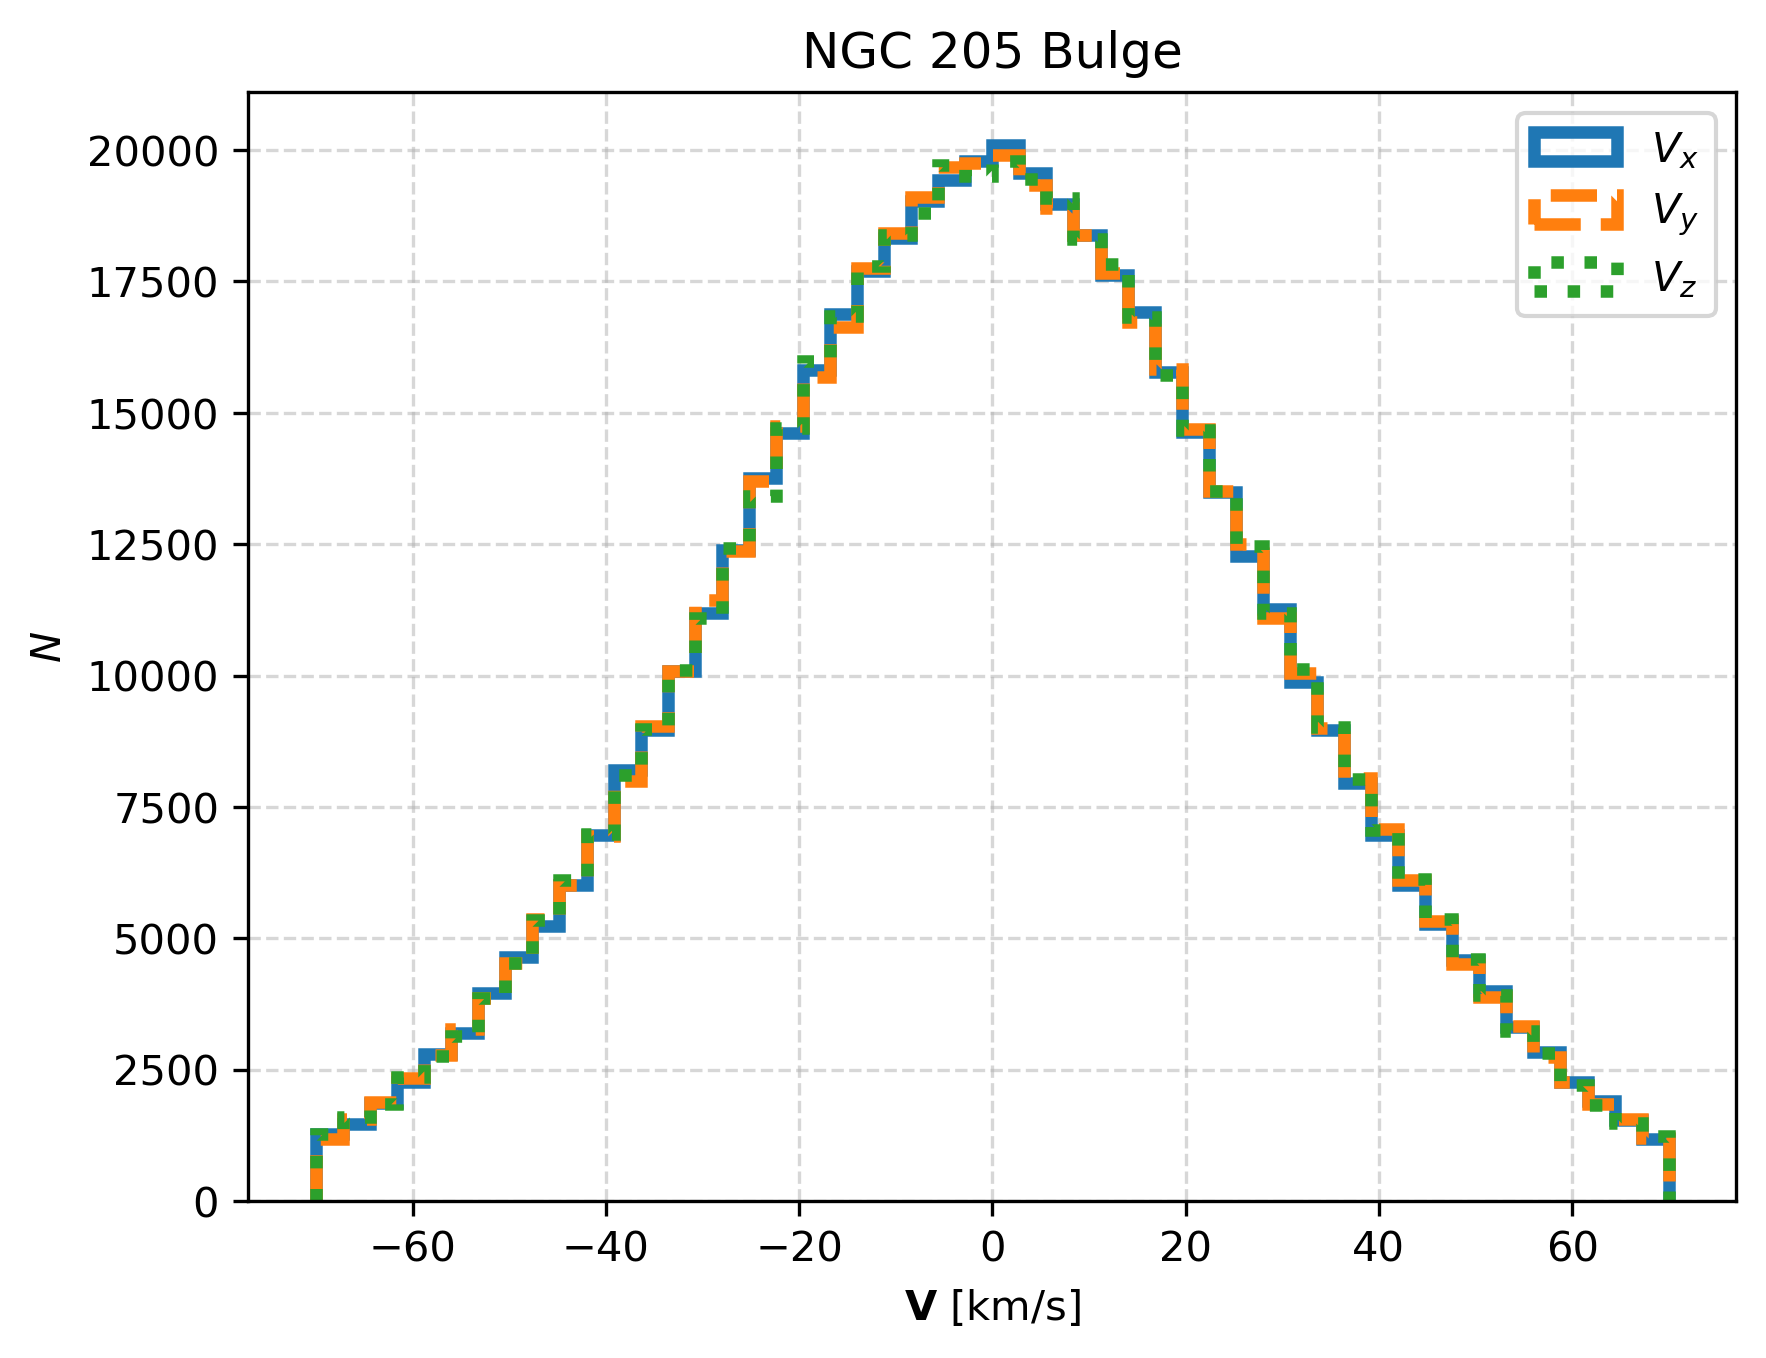
\includegraphics[width=\linewidth]{NGC205_bulge_velocity_hist.png}
        \caption{A}
    \end{subfigure}
    \hfill
    \begin{subfigure}{0.3\textwidth}
        \centering
        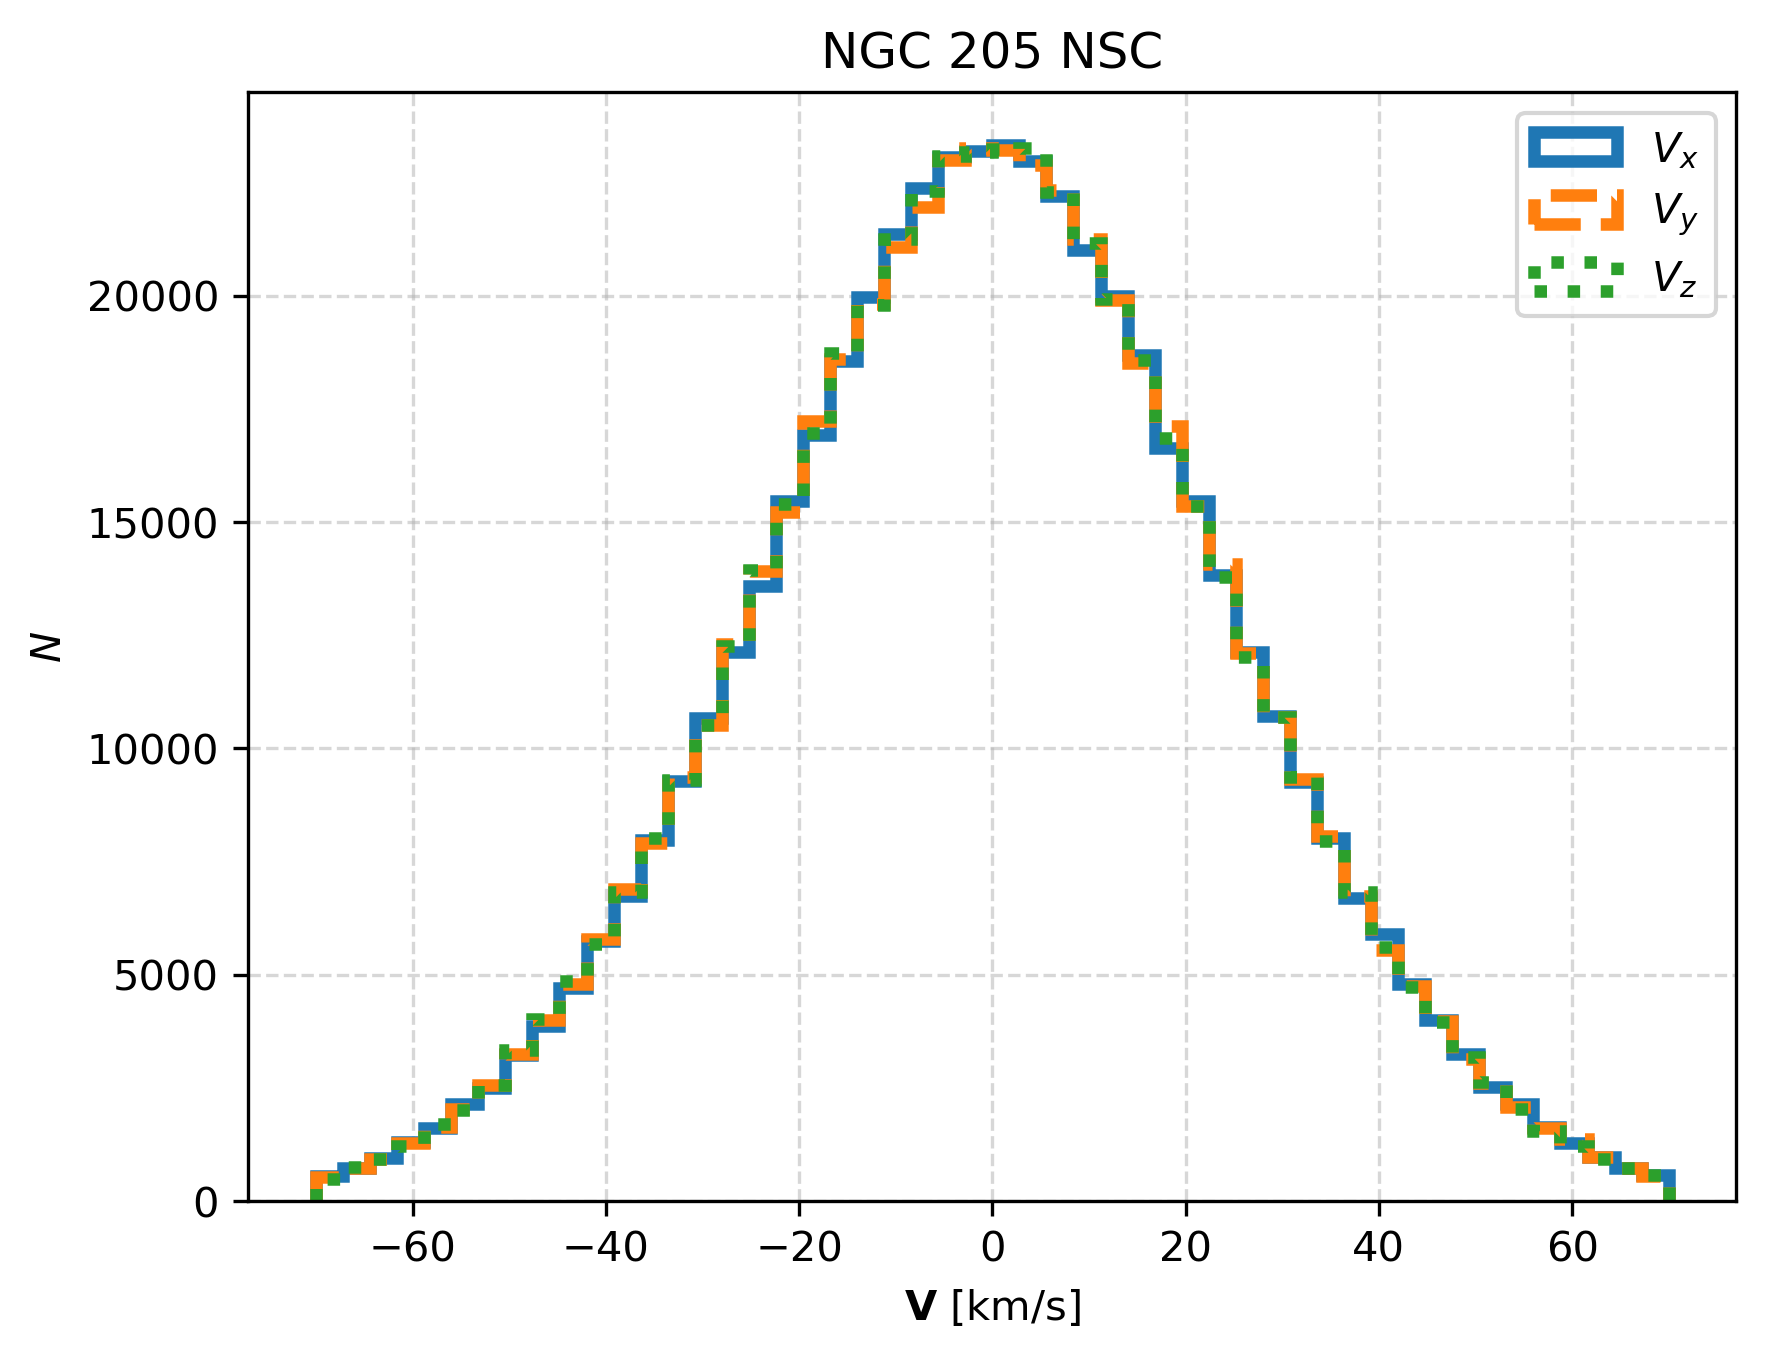
\includegraphics[width=\linewidth]{NGC205_NSC_velocity_hist.png}
        \caption{B}
    \end{subfigure}
    \hfill
    \begin{subfigure}{0.3\textwidth}
        \centering
        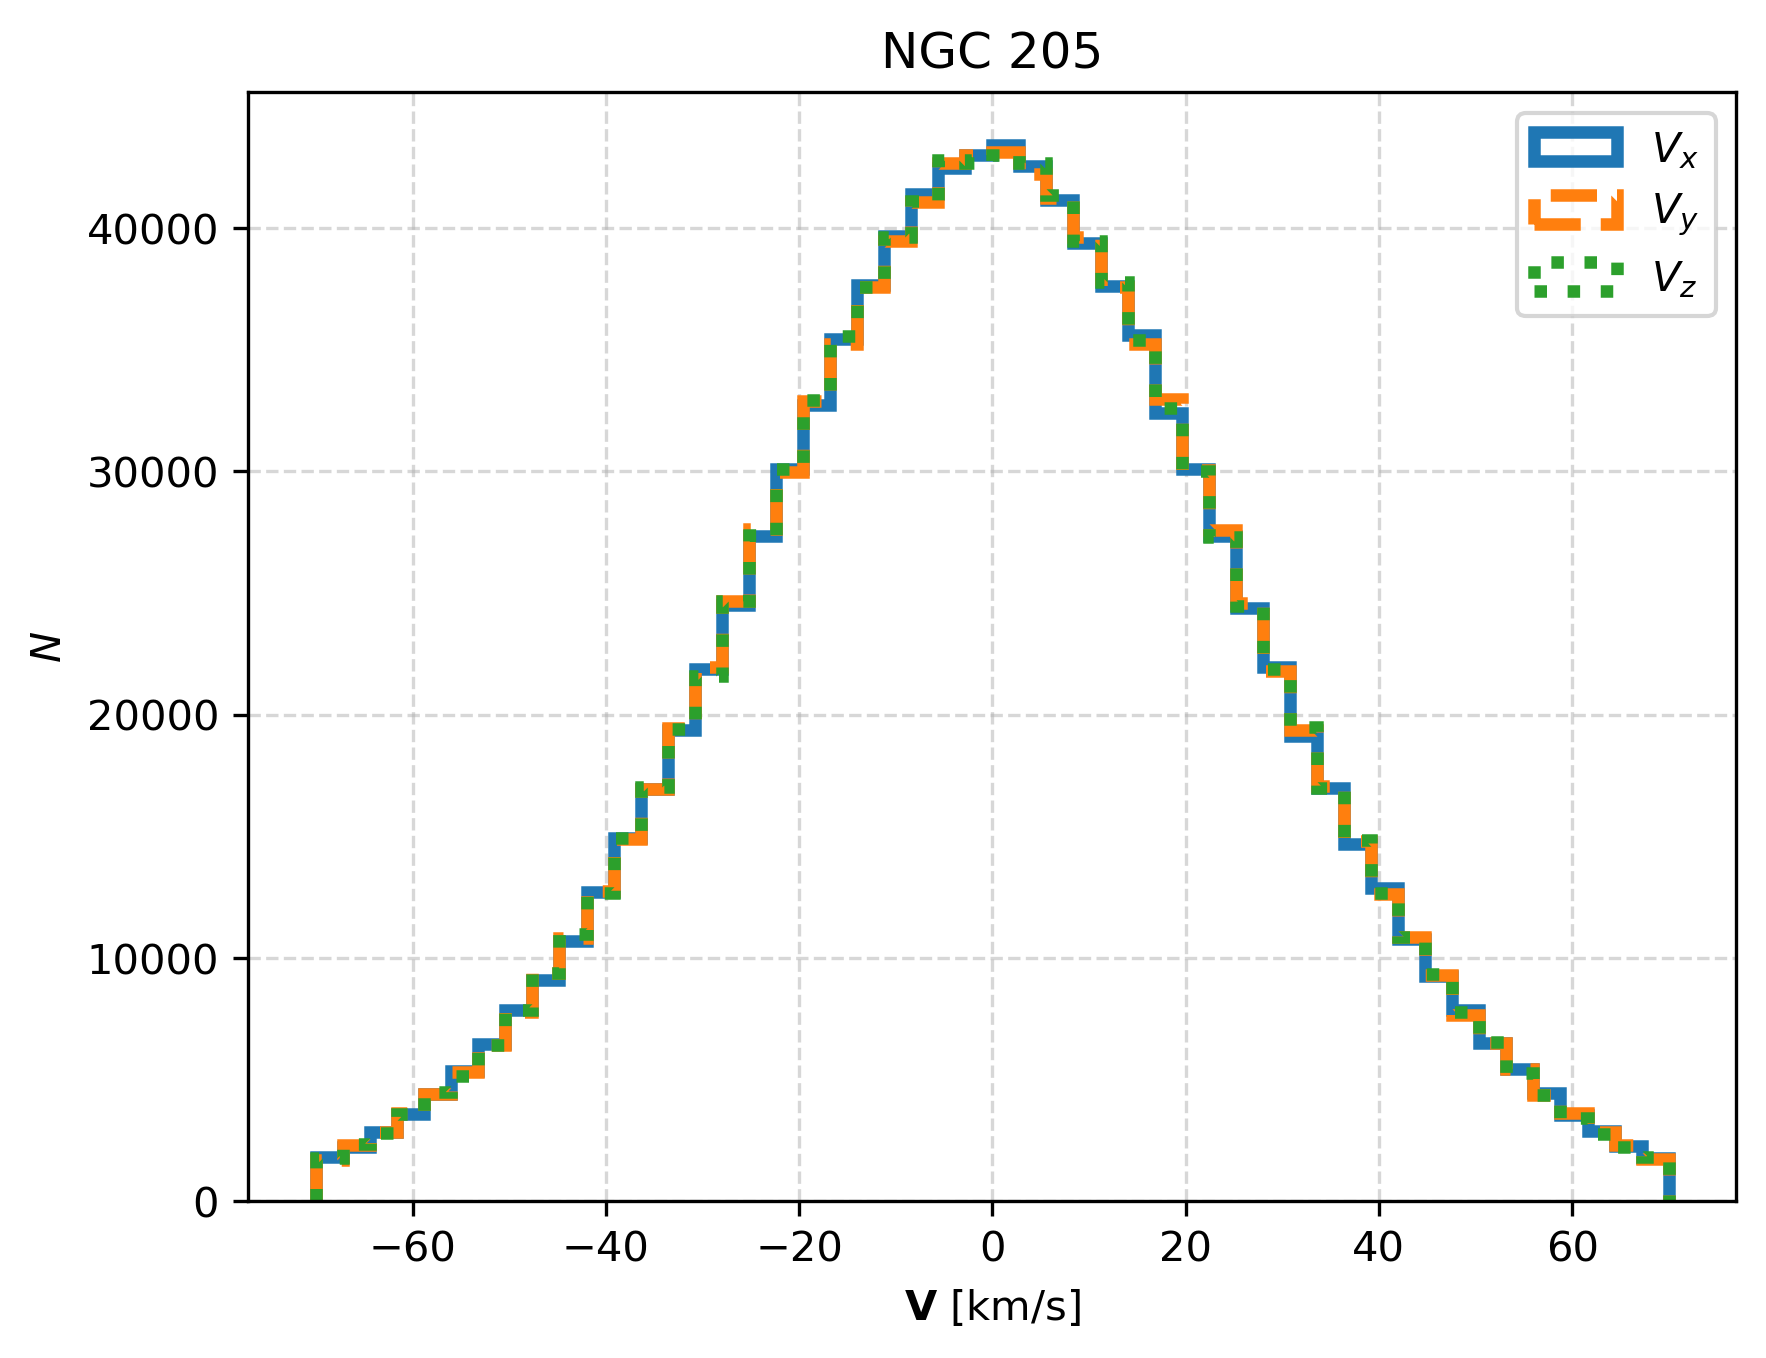
\includegraphics[width=\linewidth]{NGC205_velocity_hist.png}
        \caption{C}
    \end{subfigure}
    
    \caption{aaa}
    \label{3 NGC205_velocity_hist}
\end{figure}

\begin{figure}[h]
\centering
 \begin{subfigure}{0.3\textwidth}
        \centering
        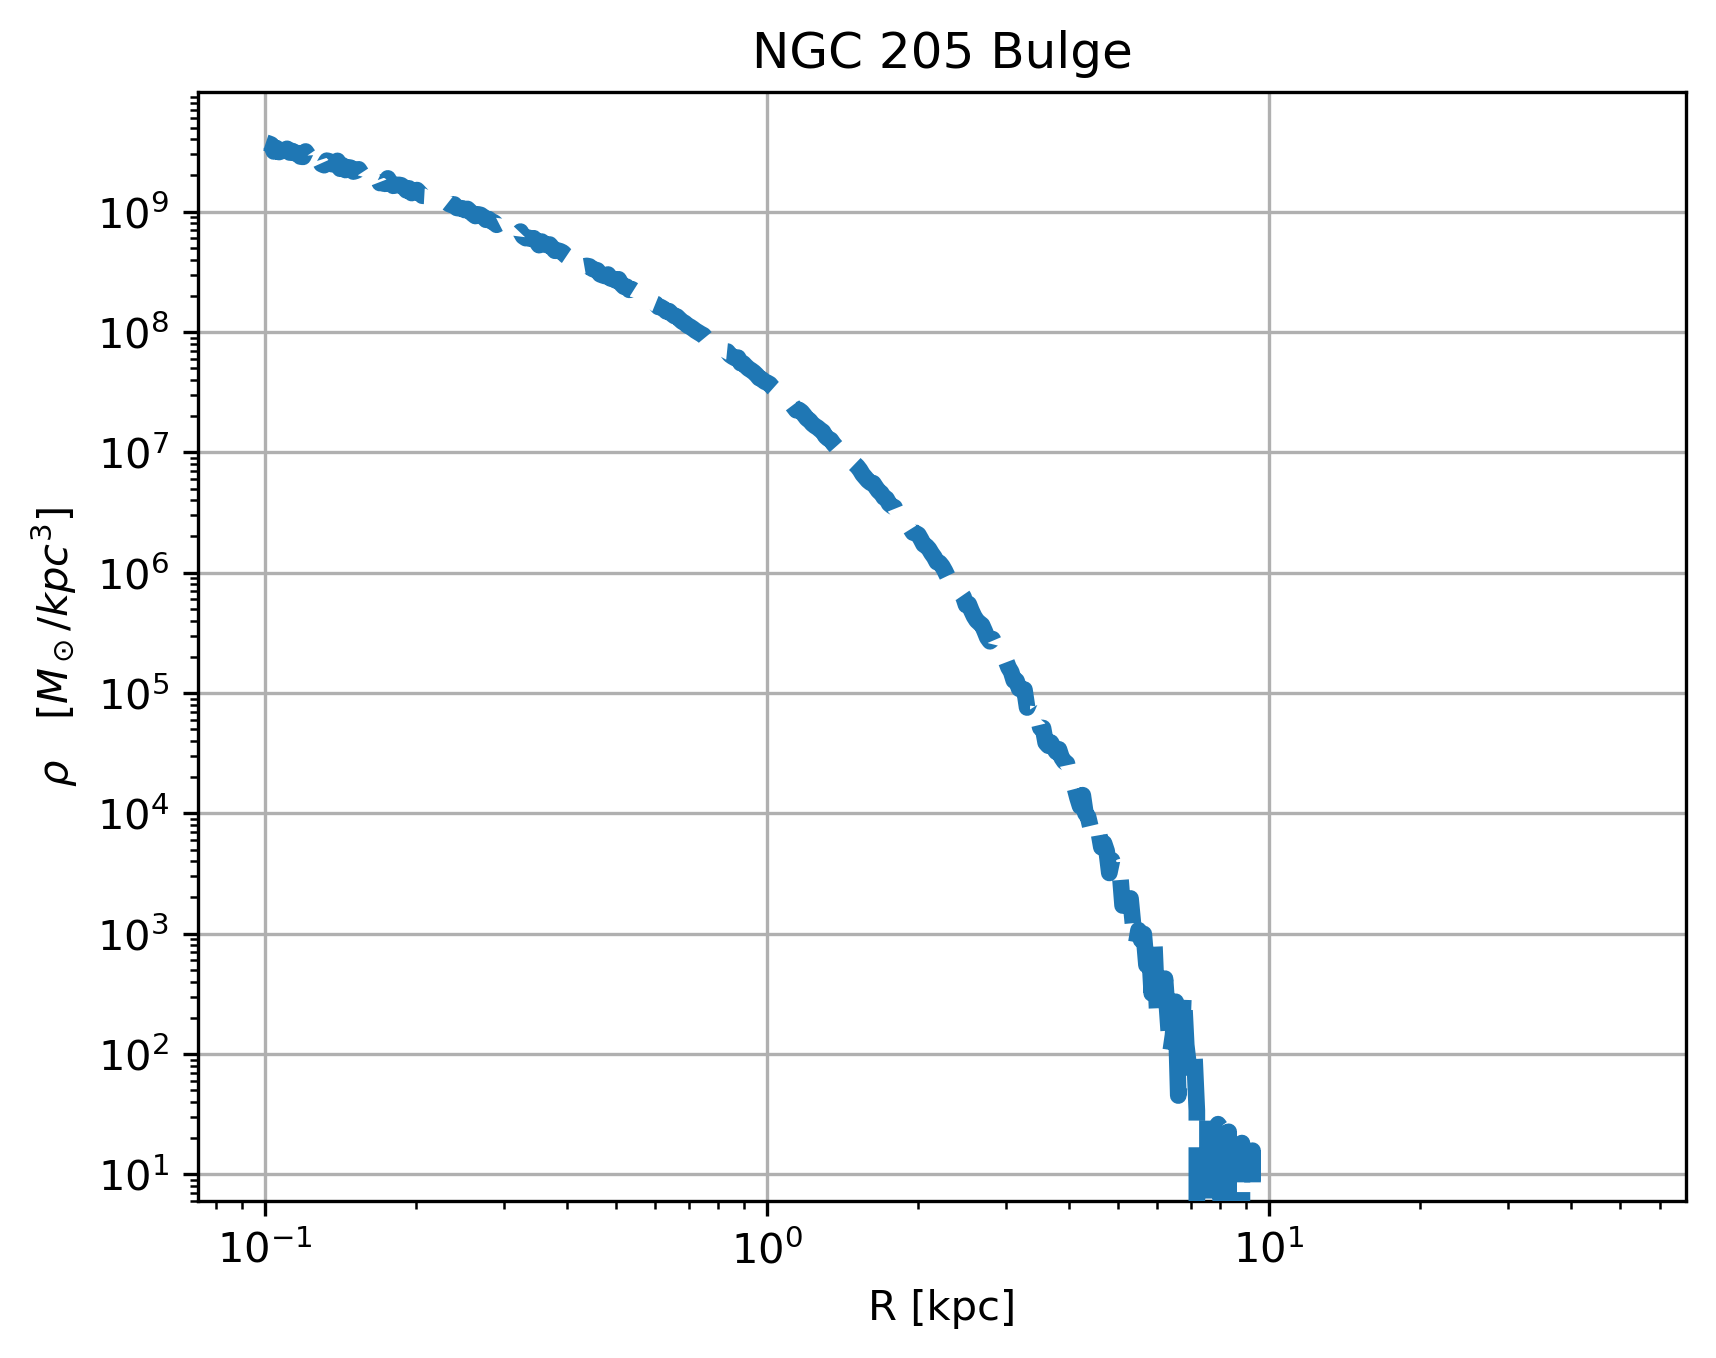
\includegraphics[width=\linewidth]{NGC205_bulge_density_Nbody.png}
        \caption{A}
    \end{subfigure}
    \hfill
    \begin{subfigure}{0.3\textwidth}
        \centering
        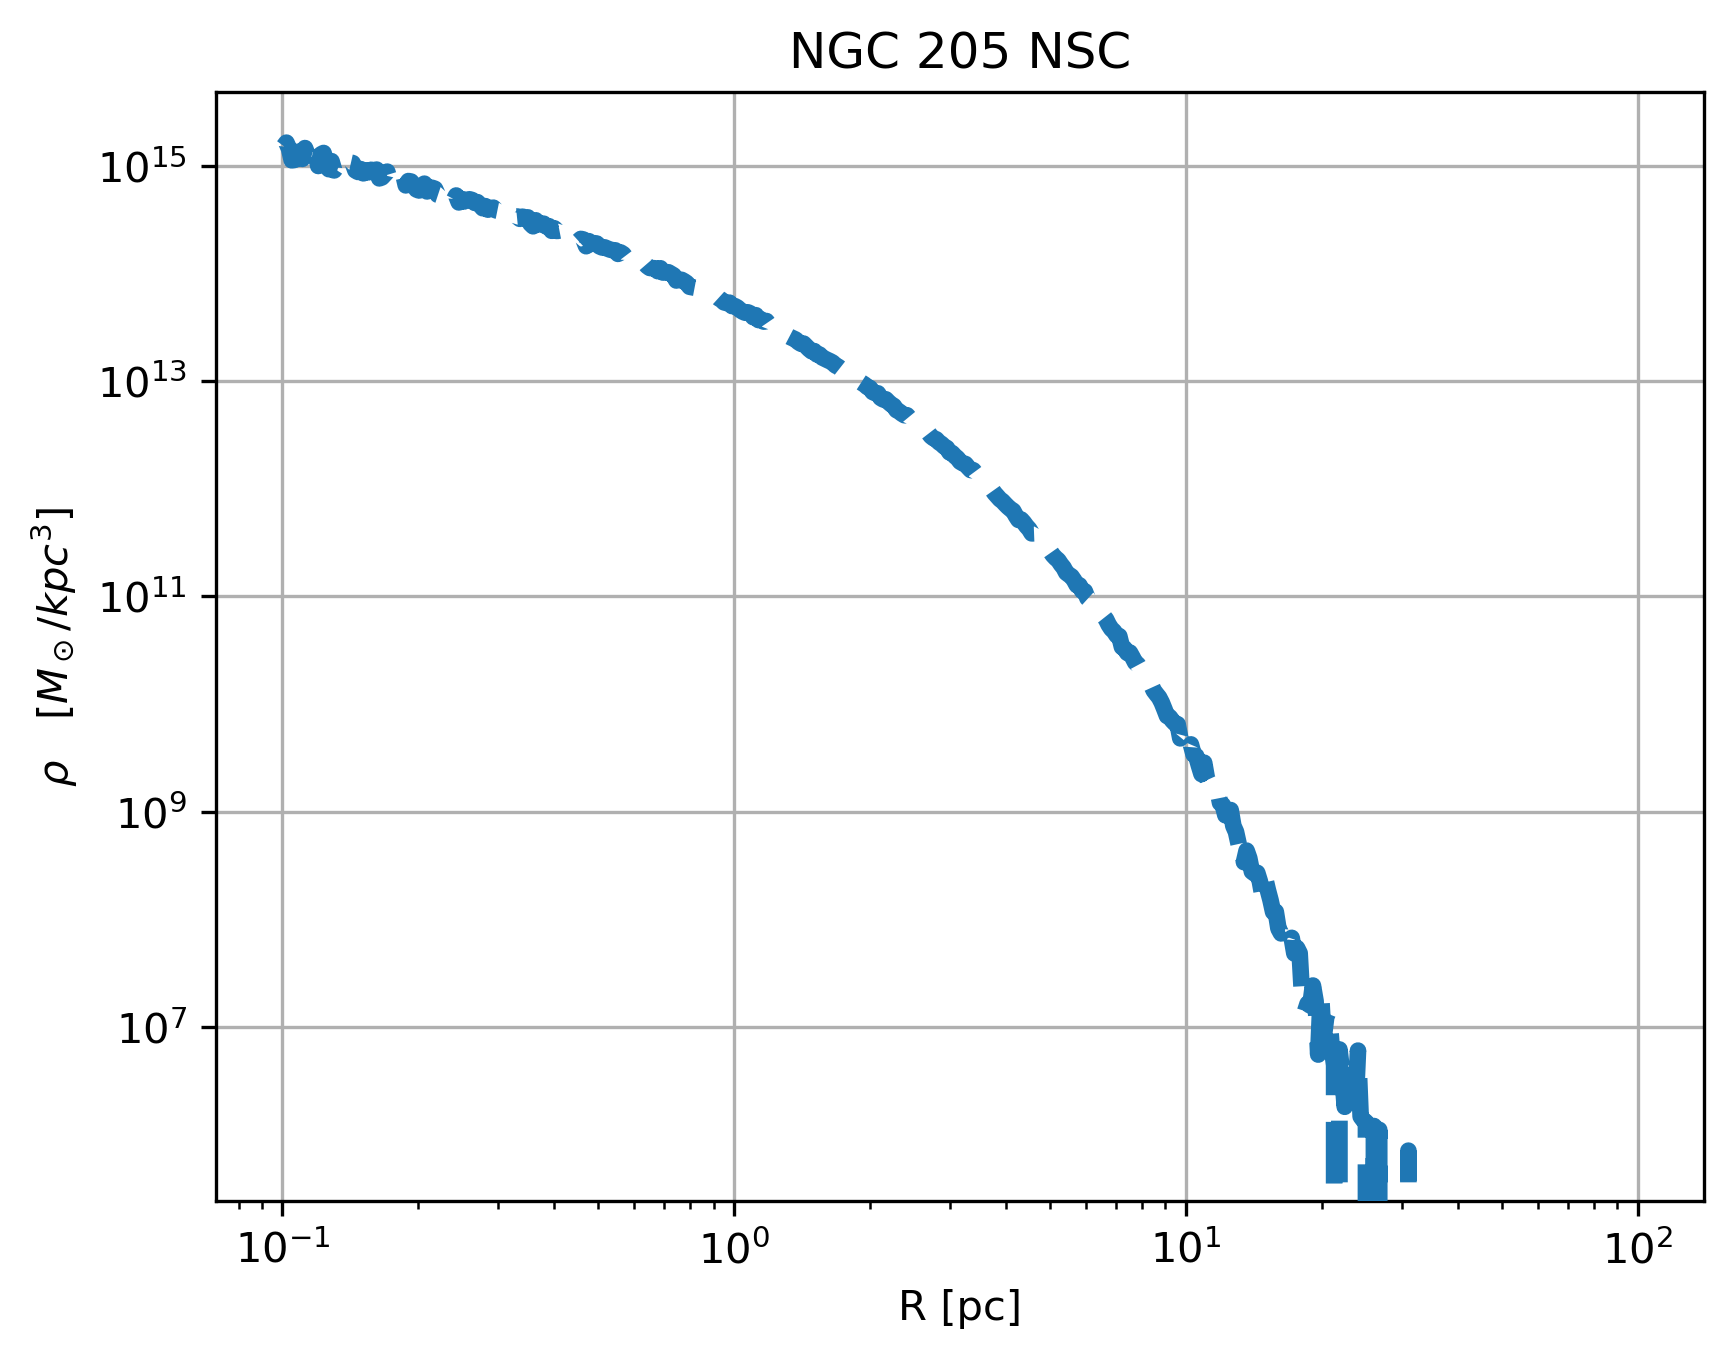
\includegraphics[width=\linewidth]{NGC205_NSC_density_Nbody.png}
        \caption{B}
    \end{subfigure}
    \hfill
    \begin{subfigure}{0.3\textwidth}
        \centering
        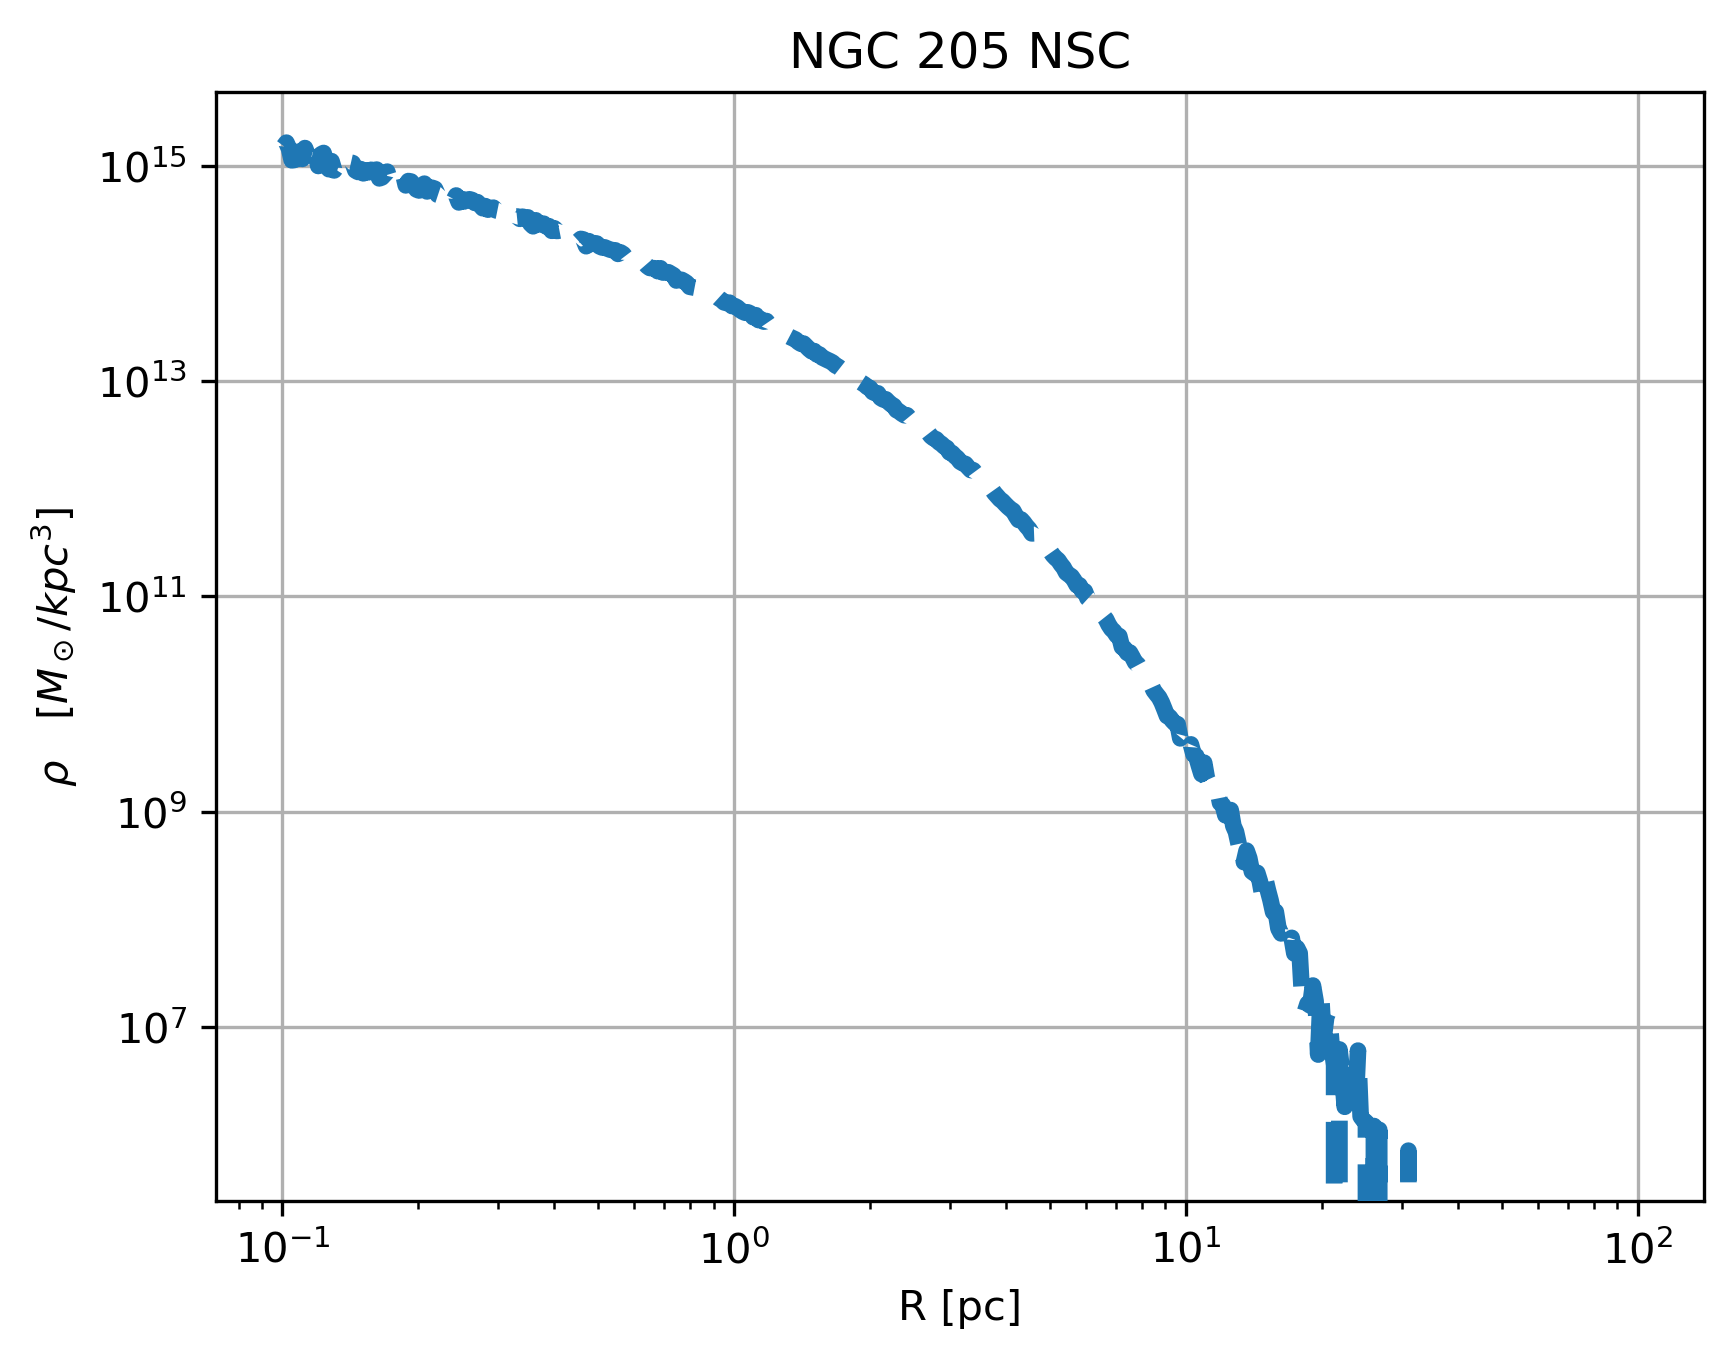
\includegraphics[width=\linewidth]{NGC205_NSC_density_Nbody.png}
        \caption{C}
    \end{subfigure}
    
    \caption{aaa}
    \label{3 NGC205_density_Nbody}
\end{figure}

\begin{figure}[h]
\centering

\begin{subfigure}{0.45\textwidth}
\centering
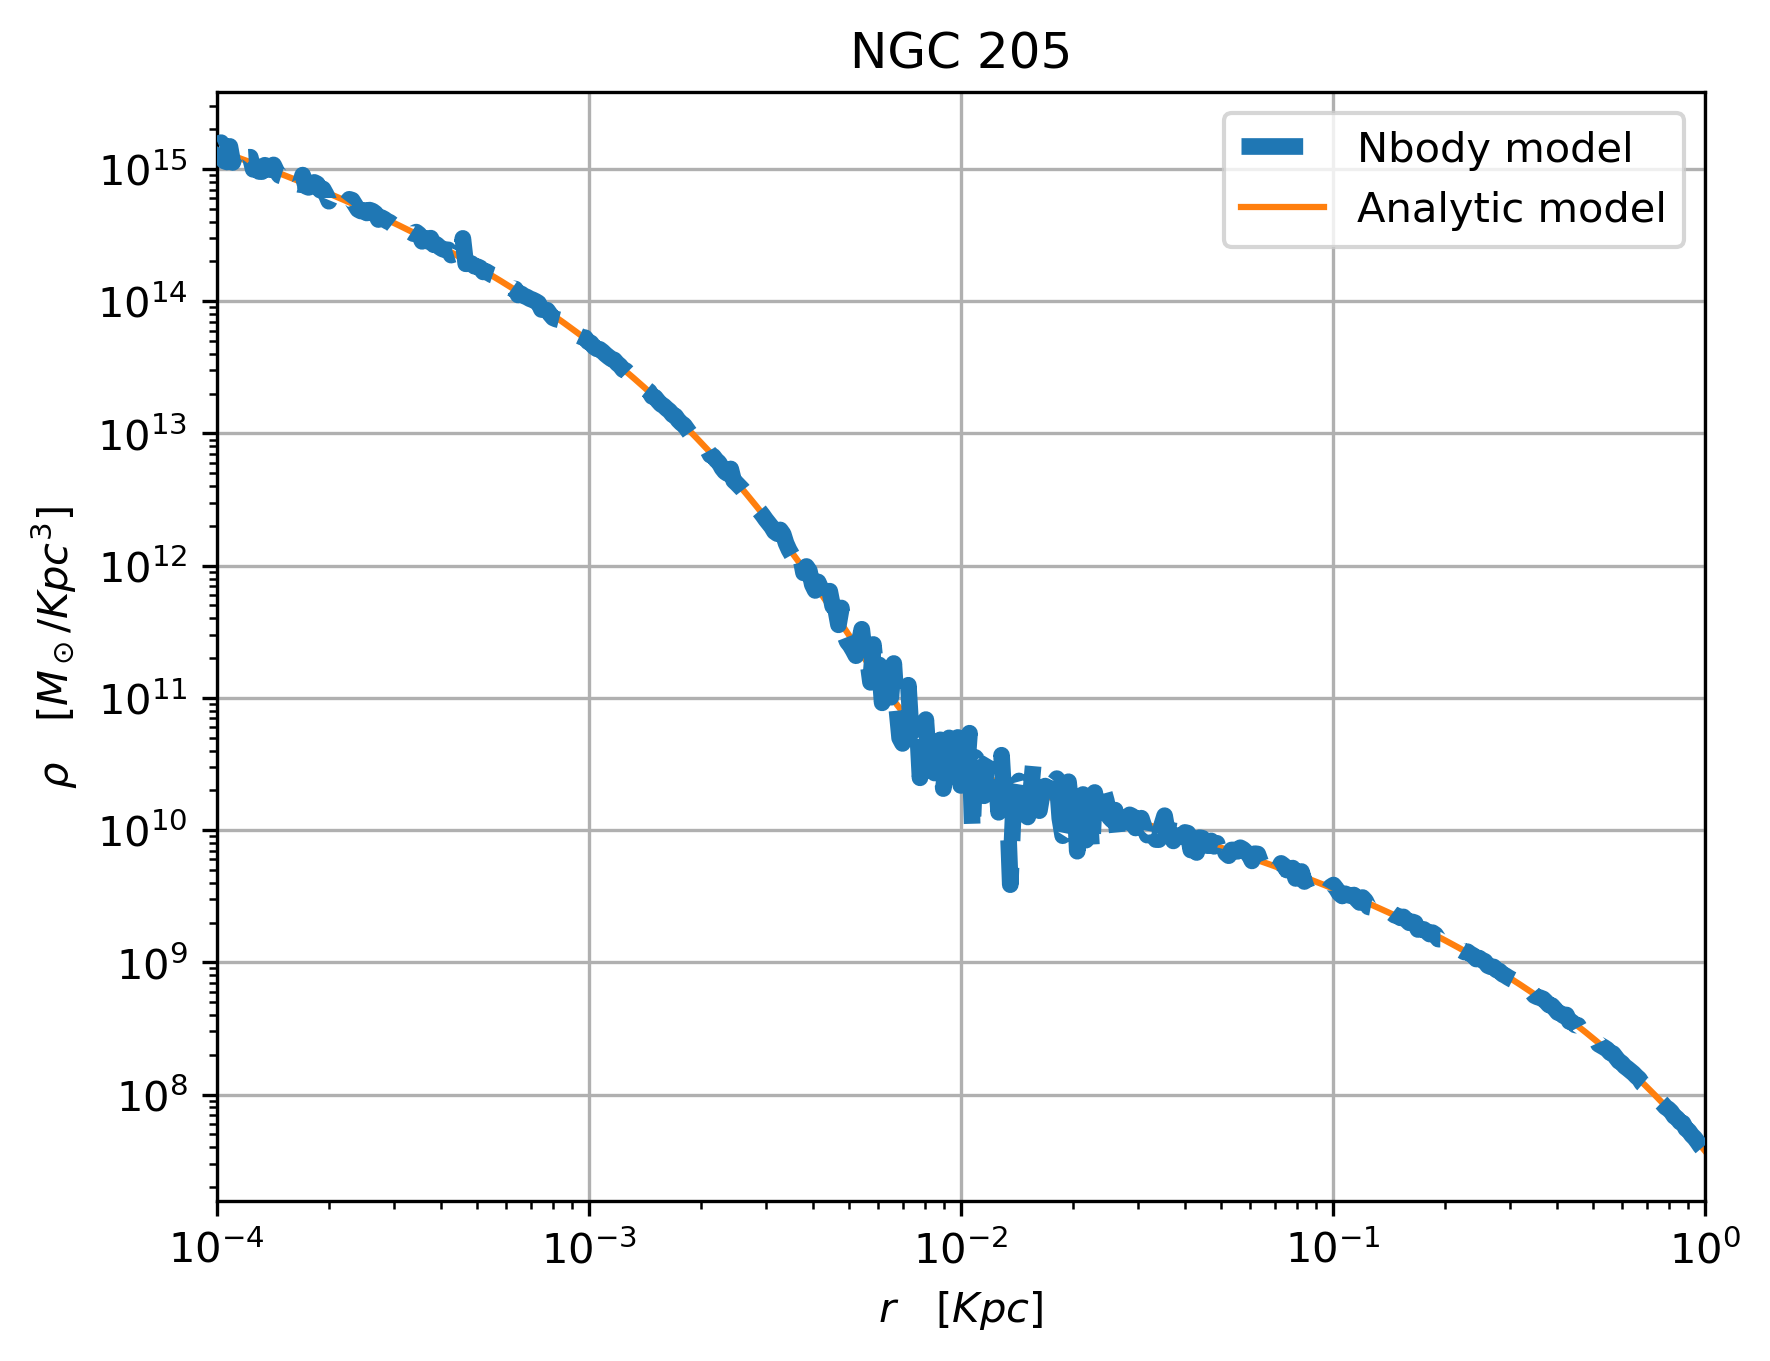
\includegraphics[width=\linewidth]{NGC205_density_Nbody_vs_analytic.png}
\caption{A}
\end{subfigure}
\hfill
\begin{subfigure}{0.45\textwidth}
\centering
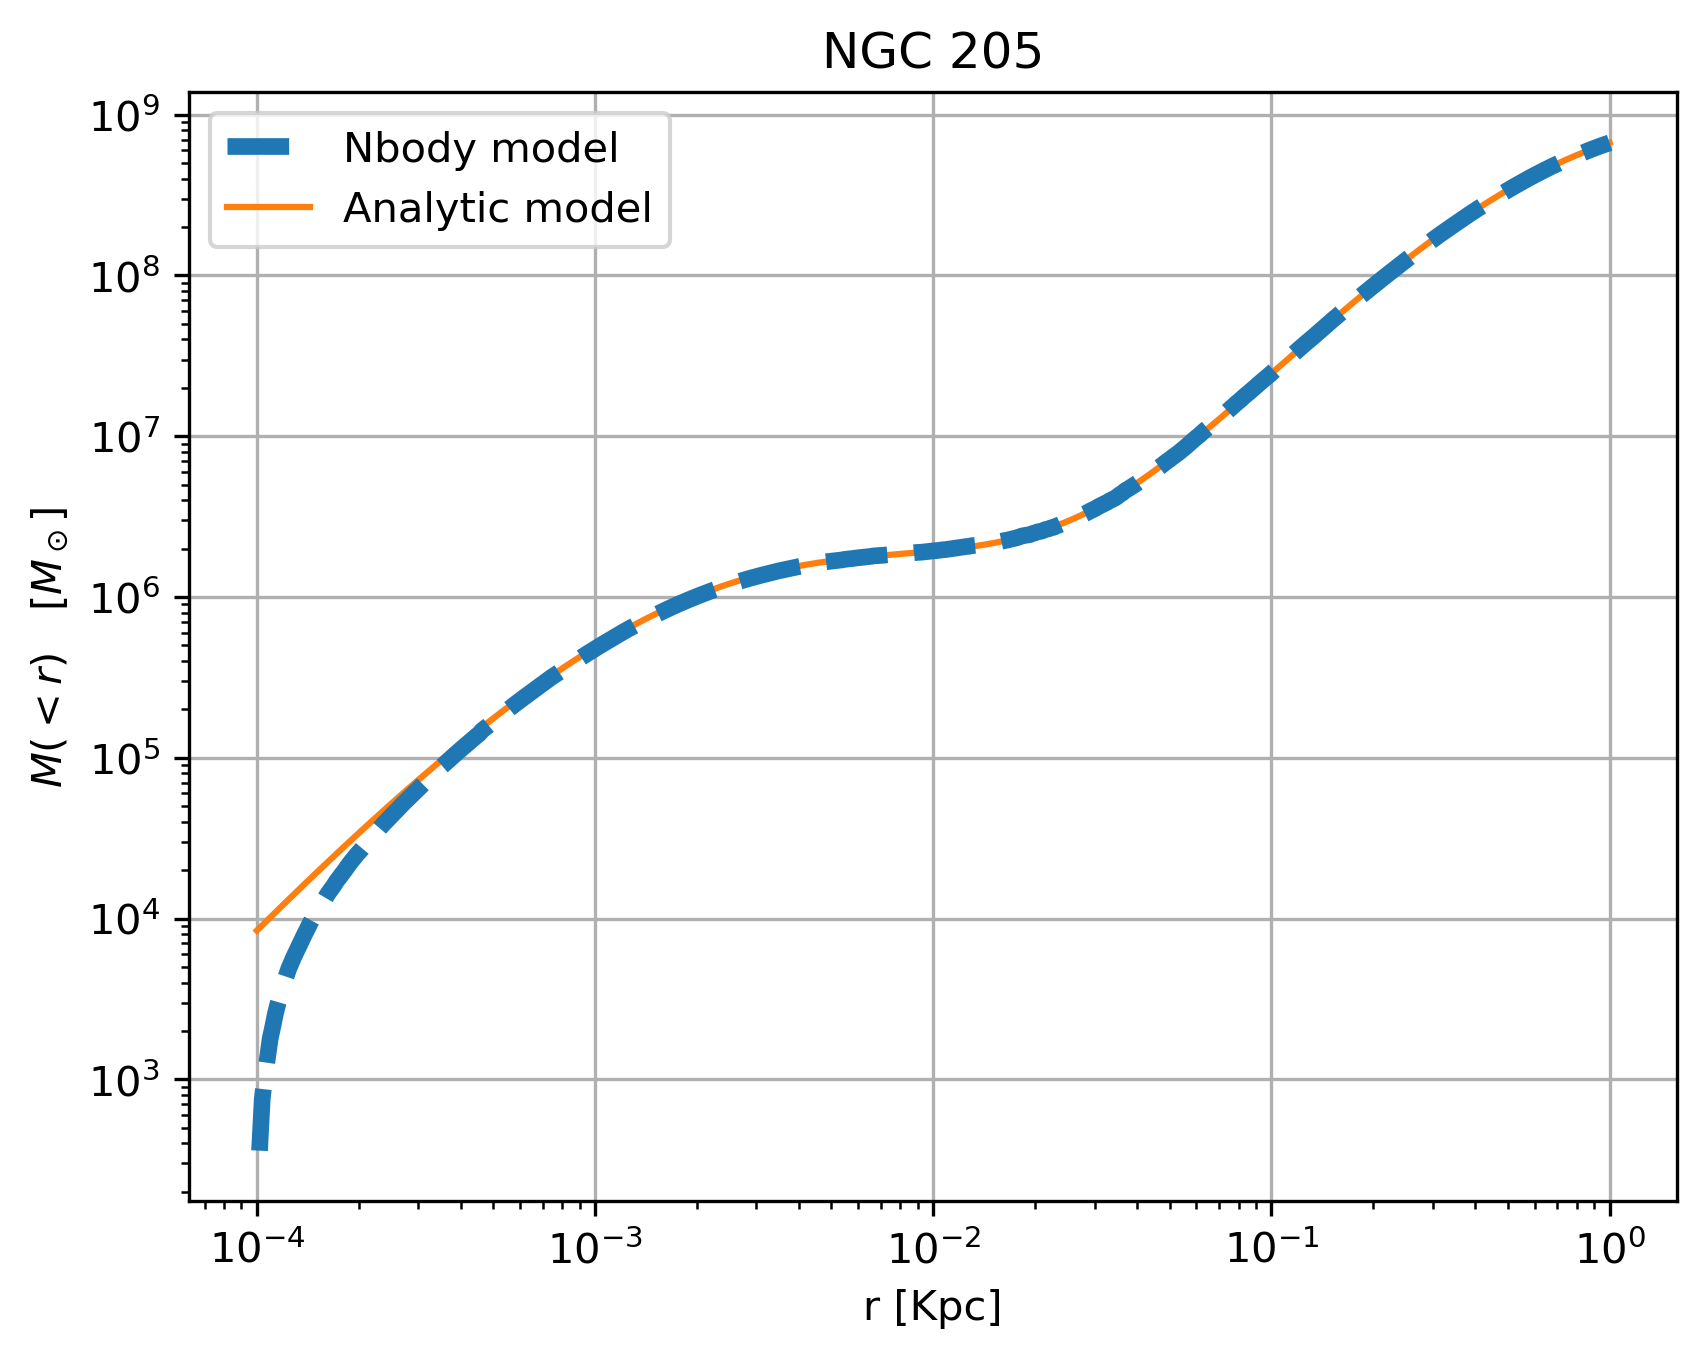
\includegraphics[width=\linewidth]{NGC205_mass_Nbody_vs_analytic.png}
\caption{B}
\end{subfigure}

\caption{aaa}
\label{NGC205 density and mass plot Nbody vs analytical}
\end{figure}

COM data:
\begin{itemize}
    \item position:
    \item velocity:
\end{itemize}

To test the stability of the Nbody generated IC, we let the system free to evolve over several
tens of the dynamical time $t_{dyn}$ at half-mass radius $r_{half}$; by definition, the former
is
\begin{equation}\label{dynamical time def}
    t_{dyn}=\frac{1}{\sqrt{G\bar{\rho}}}
\end{equation}

and the latter reads, for a spherical system,
\begin{equation}
    \bar{\rho}=\frac{M/2}{\frac{4}{3}\pi r_{half}^3}
\end{equation}

Numerically is found $r_{half}=...=... R_{eff}$.

\begin{figure}
    \centering
    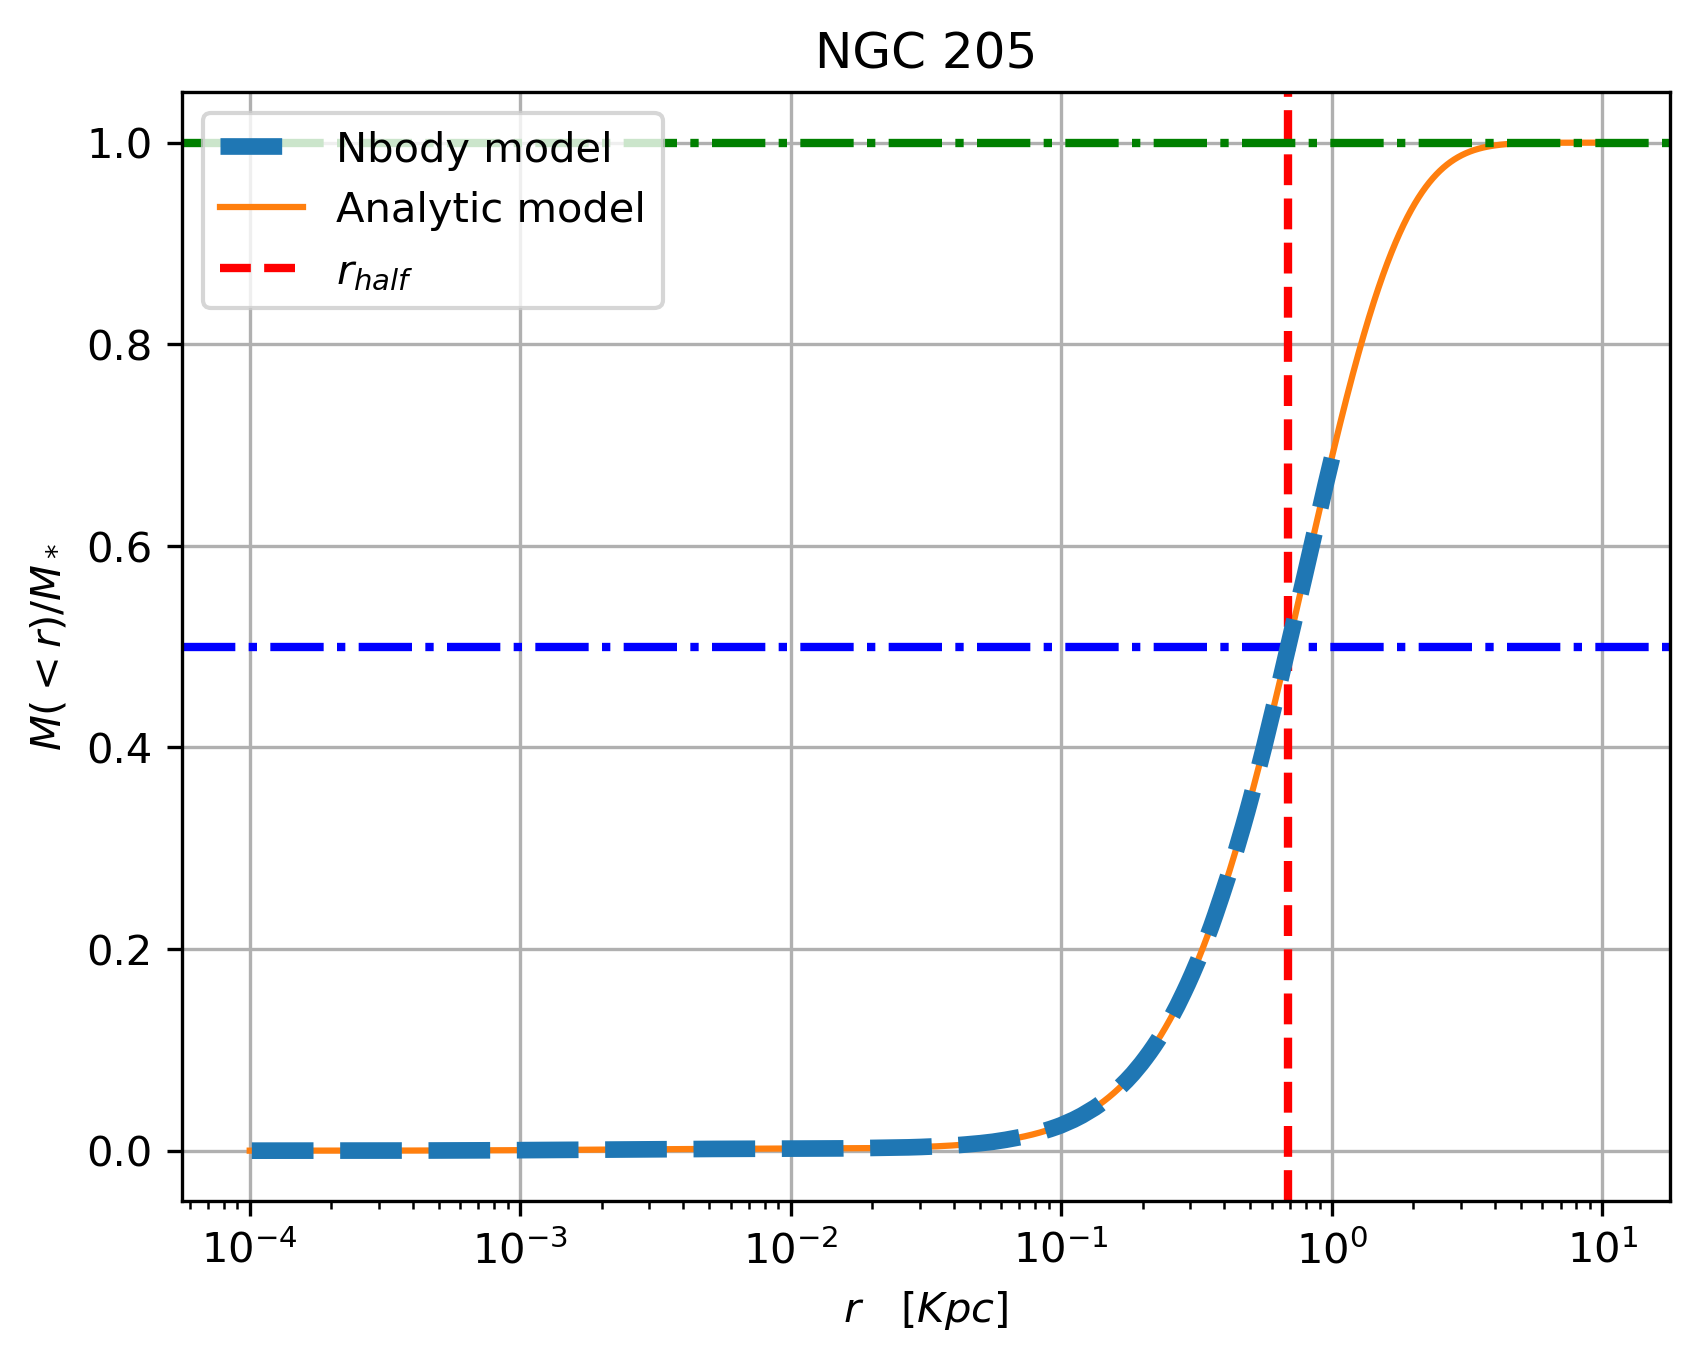
\includegraphics[width=0.5\linewidth]{NGC205_halfmass.png}
    \caption{aaa}
    \label{NGC205_halfmass}
\end{figure}
Yet, we get $t_{dyn}=...$, which agrees within $x\%$ the estimate obtained from the Analysis
tool provided by OpOpgadget, which measures this quantity directely from the generated model.
\\Waiting for evolution with Ketju.\\Additionaly, the virial ratio $Q$ has been computed as well as it gives a first indication
of whether the model is virialized, i.e. at equilibrium, or expansion/contraction operate 
within several dynamical times. In $S_{CM}$, it is defined as
\begin{equation}\label{virial ratio}
    Q=\frac{2K}{|U|}
\end{equation}
where
\begin{equation}
K = \sum_{i=1}^{N} \frac{1}{2} m_i v_i^2
\end{equation}
and
\begin{equation}
U = -\frac{1}{2} \sum_{i=1}^{N} \sum_{j \ne i} \frac{Gm_i m_j}{|\mathbf{x_i}-\mathbf{x_j}|}
\end{equation}
stand for the total kinetic and gravitational potential energies respsectively.
\\By erasing the offset due the COM kinetic energy contribute, i.e.
\begin{equation}\label{virial ratio without offset}
    Q=\frac{2(K-K_{CM})}{|U|}
\end{equation}
it is found $Q=x$.














\appendix
\renewcommand{\cftchappresnum}{APPENDIX~}
\renewcommand{\cftchapnumwidth}{9em}

\chapter{Physics Equation}

\chapter{Numerical Methods}
\section{Runge-Kutta (4)}
Given the first order autonomous ODE 
\begin{equation}
    \frac{du}{dt}=f(u),
\end{equation}
the stability anylisis of RK (4) applied to this equation leads to the following stability criterion on the time step size when $f(u)=au$:
\begin{equation}\label{RK (4) stability}
    \Delta t \le \frac{2.79}{|a|}.
\end{equation}
A system of first order autonomous ODEs can be written in vectorial form as:
\begin{equation}
    \mathbf{u}'=\mathbf{f}(\mathbf{u}).
\end{equation}
At linear order, the stability analysis we are allowed to perform the stability analysis to the linearized system
\begin{equation}
    \delta \mathbf{u}'=\mathbf{J}\delta \mathbf{u},
\end{equation}
where $\lambda_i$ is the i-th eigenvalue of the jacobian matrix $\mathbf{J}=\partial \mathbf{f}/\partial \mathbf{u}$.\\In the eigenvectors frame, equations look like
\begin{equation}
    \delta u'_i=\lambda_i\delta u_i\qquad\forall i=1,N
\end{equation}
and according to Equation (\ref{RK (4) stability}), one would get 
\begin{equation}
    \Delta t_i \le \frac{2.79}{|\lambda_i|} \qquad \forall i=1,N.
\end{equation}
Therefore, for a system of N Equations, a proper choice of the time step should be
\begin{equation}
    \Delta t=\epsilon \cdot min\left \{\frac{2.79}{|\lambda_i|}\right\} \qquad \forall i=1,N
\end{equation}
with $\epsilon\le 1$.



\printbibliography


\end{document}